\documentclass[graybox,envcountchap,sectrefs]{svmono_mod}
%\documentclass[envcountsame,envcountchap]{svmono}

% choose options for [] as required from the list
% in the Reference Guide
\usepackage{amsmath}
\usepackage{amsfonts}
\usepackage{amssymb}
\usepackage{mathptmx}
\usepackage{helvet}
\usepackage{courier}
%
\usepackage{type1cm}         
%\usepackage{epsfig}
\usepackage{makeidx}         % allows index generation
\usepackage{graphicx}        % standard LaTeX graphics tool
                             % when including figure files
\graphicspath{{Figures/}}
\usepackage{multicol}        % used for the two-column index
\usepackage[bottom]{footmisc}% places footnotes at page bottom
\usepackage{array,booktabs,calc}

\usepackage{listings}
\usepackage[final]{pdfpages}
% see the list of further useful packages
% in the Reference Guide

%\usepackage{anyfontsize}
\usepackage{enumerate}
%\usepackage{rotating}
%\usepackage{psfrag}
%\usepackage{color}
%\usepackage{framed}
%\usepackage{t1enc}
%\usepackage{times}
%\usepackage{fancyhdr}
%\usepackage{float}
%\usepackage{marvosym}
\usepackage{tikz,pgfplots}
\usetikzlibrary{arrows.meta,quotes}
%\usepackage[mode=tex]{standalone}
\usepackage[mode=buildnew]{standalone}

%1)The following piece of code has been taken from the Internet and redefines the \widebar command to make it look better (and better than overline)
\makeatletter
\let\save@mathaccent\mathaccent
\newcommand*\if@single[3]{%
  \setbox0\hbox{${\mathaccent"0362{#1}}^H$}%
  \setbox2\hbox{${\mathaccent"0362{\kern0pt#1}}^H$}%
  \ifdim\ht0=\ht2 #3\else #2\fi
  }
%The bar will be moved to the right by a half of \macc@kerna, which is computed by amsmath:
\newcommand*\rel@kern[1]{\kern#1\dimexpr\macc@kerna}
%If there's a superscript following the bar, then no negative kern may follow the bar;
%an additional {} makes sure that the superscript is high enough in this case:
\newcommand*\widebar[1]{\@ifnextchar^{{\wide@bar{#1}{0}}}{\wide@bar{#1}{1}}}
%Use a separate algorithm for single symbols:
\newcommand*\wide@bar[2]{\if@single{#1}{\wide@bar@{#1}{#2}{1}}{\wide@bar@{#1}{#2}{2}}}
\newcommand*\wide@bar@[3]{%
  \begingroup
  \def\mathaccent##1##2{%
%Enable nesting of accents:
    \let\mathaccent\save@mathaccent
%If there's more than a single symbol, use the first character instead (see below):
    \if#32 \let\macc@nucleus\first@char \fi
%Determine the italic correction:
    \setbox\z@\hbox{$\macc@style{\macc@nucleus}_{}$}%
    \setbox\tw@\hbox{$\macc@style{\macc@nucleus}{}_{}$}%
    \dimen@\wd\tw@
    \advance\dimen@-\wd\z@
%Now \dimen@ is the italic correction of the symbol.
    \divide\dimen@ 3
    \@tempdima\wd\tw@
    \advance\@tempdima-\scriptspace
%Now \@tempdima is the width of the symbol.
    \divide\@tempdima 10
    \advance\dimen@-\@tempdima
%Now \dimen@ = (italic correction / 3) - (Breite / 10)
    \ifdim\dimen@>\z@ \dimen@0pt\fi
%The bar will be shortened in the case \dimen@<0 !
    \rel@kern{0.6}\kern-\dimen@
    \if#31
      \overline{\rel@kern{-0.6}\kern\dimen@\macc@nucleus\rel@kern{0.4}\kern\dimen@}%
      \advance\dimen@0.4\dimexpr\macc@kerna
%Place the combined final kern (-\dimen@) if it is >0 or if a superscript follows:
      \let\final@kern#2%
      \ifdim\dimen@<\z@ \let\final@kern1\fi
      \if\final@kern1 \kern-\dimen@\fi
    \else
      \overline{\rel@kern{-0.6}\kern\dimen@#1}%
    \fi
  }%
  \macc@depth\@ne
  \let\math@bgroup\@empty \let\math@egroup\macc@set@skewchar
  \mathsurround\z@ \frozen@everymath{\mathgroup\macc@group\relax}%
  \macc@set@skewchar\relax
  \let\mathaccentV\macc@nested@a
%The following initialises \macc@kerna and calls \mathaccent:
  \if#31
    \macc@nested@a\relax111{#1}%
  \else
%If the argument consists of more than one symbol, and if the first token is
%a letter, use that letter for the computations:
    \def\gobble@till@marker##1\endmarker{}%
    \futurelet\first@char\gobble@till@marker#1\endmarker
    \ifcat\noexpand\first@char A\else
      \def\first@char{}%
    \fi
    \macc@nested@a\relax111{\first@char}%
  \fi
  \endgroup
}
\makeatother








%%% 2) Operadores de decision
\def\dunodcero{\begin{array}{c} D=1 \\ \gtrless \\ D=0 \end{array}}
\def\dceroduno{\begin{array}{c} D=0 \\ \gtrless \\ D=1 \end{array}}
%%%
%%% 3) Abreviaturas para PFA, PM  y PD.
\newcommand{\pfa}{P_{\text{FA}}} 
\newcommand{\pmis}{P_{\text{M}}} 
\newcommand{\pdet}{P_{\text{D}}} 
\newcommand{\appropto}{\mathrel{\vcenter{\offinterlineskip\halign{\hfil$##$\cr \propto\cr\noalign{\kern2pt}\sim\cr\noalign{\kern-2pt}}}}}

\makeindex             % used for the subject index
                       % please use the style svind.ist with
                       % your makeindex program

%%%%%%%%%%%%%%%%%%%%%%%%%%%%%%%%%%%%%%%%%%%%%%%%%%%%%%%%%%%%%%%%%%%%%
\newcommand{\px}{p_X(x)}
\newcommand{\py}{p_Y(y)}

\begin{document}

\author{Jer\'onimo Arenas-Garc\'ia, Jes\'us Cid-Sueiro, Vanessa G\'omez-Verdejo, Miguel L\'azaro-Gredilla, and David Ram{\'\i}rez}
\title{Estimation and Detection Theory}
\subtitle{Year 2020-21}
\maketitle

\frontmatter%%%%%%%%%%%%%%%%%%%%%%%%%%%%%%%%%%%%%%%%%%%%%%%%%%%%%%

%%%%%%%%%%%%%%%%%%%%%%%% dedic.tex %%%%%%%%%%%%%%%%%%%%%%%%%%%%%%%%%
%
% sample dedication
%
% Use this file as a template for your own input.
%
%%%%%%%%%%%%%%%%%%%%%%%% Springer %%%%%%%%%%%%%%%%%%%%%%%%%%

\begin{dedication}
Use the template \emph{dedic.tex} together with the Springer document class SVMono for monograph-type books or SVMult for contributed volumes to style a quotation or a dedication\index{dedication} at the very beginning of your book in the Springer layout
\end{dedication}





%%%%%%%%%%%%%%%%%%%%%%%foreword.tex%%%%%%%%%%%%%%%%%%%%%%%%%%%%%%%%%
% sample foreword
%
% Use this file as a template for your own input.
%
%%%%%%%%%%%%%%%%%%%%%%%% Springer %%%%%%%%%%%%%%%%%%%%%%%%%%

\foreword

%% Please have the foreword written here
Use the template \textit{foreword.tex} together with the Springer document class SVMono (monograph-type books) or SVMult (edited books) to style your foreword\index{foreword} in the Springer layout. 

The foreword covers introductory remarks preceding the text of a book that are written by a \textit{person other than the author or editor} of the book. If applicable, the foreword precedes the preface which is written by the author or editor of the book.


\vspace{\baselineskip}
\begin{flushright}\noindent
Place, month year\hfill {\it Firstname  Surname}\\
\end{flushright}



%%%%%%%%%%%%%%%%%%%%%%%preface.tex%%%%%%%%%%%%%%%%%%%%%%%%%%%%%%%%%%%%%%%%%
% sample preface
%
% Use this file as a template for your own input.
%
%%%%%%%%%%%%%%%%%%%%%%%% Springer %%%%%%%%%%%%%%%%%%%%%%%%%%

\preface

%% Please write your preface here
Use the template \emph{preface.tex} together with the Springer document class SVMono (monograph-type books) or SVMult (edited books) to style your preface in the Springer layout.

A preface\index{preface} is a book's preliminary statement, usually written by the \textit{author or editor} of a work, which states its origin, scope, purpose, plan, and intended audience, and which sometimes includes afterthoughts and acknowledgments of assistance. 

When written by a person other than the author, it is called a foreword. The preface or foreword is distinct from the introduction, which deals with the subject of the work.

Customarily \textit{acknowledgments} are included as last part of the preface.
 

\vspace{\baselineskip}
\begin{flushright}\noindent
Place(s),\hfill {\it Firstname  Surname}\\
month year\hfill {\it Firstname  Surname}\\
\end{flushright}



%%%%%%%%%%%%%%%%%%%%%%%acknow.tex%%%%%%%%%%%%%%%%%%%%%%%%%%%%%%%%%%%%%%%%%
% sample acknowledgement chapter
%
% Use this file as a template for your own input.
%
%%%%%%%%%%%%%%%%%%%%%%%% Springer %%%%%%%%%%%%%%%%%%%%%%%%%%

\extrachap{Acknowledgements}

Use the template \emph{acknow.tex} together with the Springer document class SVMono (monograph-type books) or SVMult (edited books) if you prefer to set your acknowledgement section as a separate chapter instead of including it as last part of your preface.



%\pagestyle{empty}

\tableofcontents
%%%%%%%%%%%%%%%%%%%%%%%acronym.tex%%%%%%%%%%%%%%%%%%%%%%%%%%%%%%%%%%%%%%%%%
% sample list of acronyms
%
% Use this file as a template for your own input.
%
%%%%%%%%%%%%%%%%%%%%%%%% Springer %%%%%%%%%%%%%%%%%%%%%%%%%%

\extrachap{Acronyms}

Use the template \emph{acronym.tex} together with the Springer document class SVMono (monograph-type books) or SVMult (edited books) to style your list(s) of abbreviations or symbols in the Springer layout.

Lists of abbreviations\index{acronyms, list of}, symbols\index{symbols, list of} and the like are easily formatted with the help of the Springer-enhanced \verb|description| environment.

\begin{description}[CABR]
\item[ABC]{Spelled-out abbreviation and definition}
\item[BABI]{Spelled-out abbreviation and definition}
\item[CABR]{Spelled-out abbreviation and definition}
\end{description}

\mainmatter%%%%%%%%%%%%%%%%%%%%%%%%%%%%%%%%%%%%%%%%%%%%%%%%%%%%%%%

%%%%%%%%%%%%%%%%%%%%%%part.tex%%%%%%%%%%%%%%%%%%%%%%%%%%%%%%%%%%
% 
% sample part title
%
% Use this file as a template for your own input.
%
%%%%%%%%%%%%%%%%%%%%%%%% Springer %%%%%%%%%%%%%%%%%%%%%%%%%%

\begin{partbacktext}
\part{Statistical Review}


%\noindent Use the template \emph{part.tex} together with the Springer document class SVMono (monograph-type books) or SVMult (edited books) to style your part title page and, if desired, a short introductory text (maximum one page) on its verso page in the Springer layout.

\end{partbacktext}
\chapter{Statistical Estimation Theory}
%\section{Introduction to the Estimation Problem}
\label{sec:M2}

The contents of this lesson cover an introduction to the estimation problems. So, during this session, we will present some basic concepts of estimation design using statistical information. Important concepts, such as {\em a priori} and {\em a posteriori} probabilities, observations, cost functions, or likelihoods will be illustrated through a series of simple examples.

\subsection{Example 1: Bayesian estimation without observations}
\label{subsec:example1}

\begin{problem} 
A food delivery company wants to develop a new service to estimate the time that will elapse from the reception of an order to its delivery to the customer's home.
To do this, the total service or delivery time, $S$, is modelled as a random variable given by the sum of two independent r.v.s:
$$S=T_1 + T_2,$$
where $T_1$ models the time (in minutes) needed to prepare the order and $T_2$ is the shipping time (in minutes).
Analyzing these times the company has characterized r.v.s $T_1$ and $T_2$ with the following probability distributions:

$$p_{T_1}(t_1) = 0.5 \exp{\left[-0.5(t_1 - 10) \right]} \quad \quad  t_1 >10 $$
$$p_{T_2}(t_2) = \frac{0.2}{r} \exp{\left[-\frac{0.2}{r} (t_2-5)\right]} \quad \quad  t_2 >5 $$
where r is the distance (in kilometers) from the company store to the customer's home. 
To estimate the value of $S$, let's start solving the following questions:
    \begin{itemize}
        \item[a)] Knowing the probability distributions of $T_1$ and $T_2$, can we obtain the probability distribution of $S$?
        \item[b)] Knowing the probability distribution of $S$, can we estimate the total delivery time? 
        \item[c)] Which is the optimal estimator for a given cost? 
    \end{itemize}
\end{problem}

\begin{solution} 

\begin{itemize}
\item[a)] Can we obtain the probability distribution of $S$? \\
Computing the distribution of $S$ requires applying a change of random variable in which we have to transform two random variables ($T_1$ and $T_2$) into a new variable ($S$). Since $S$ is the sum of two independent random variables, we know that their distribution will be given by the convolution of the distributions of $T_1$ and $T_2$: 
$$ p_S(s) = p_{T_1} (t_1=s) \ast  p_{T_2} (t_2=s)  = \int  p_{T_1} (t_1=s)  p_{T_2} (t_2=s-t_1) d t_1   $$
after some mathematical manipulations (the complete mathematical development is left as an exercise), we can see that $p_S(s)$ is given by the following expression (see Figure \ref{Fig_ps}):
$$ p_S(s) = \left(0.5 + \frac{0.2}{r}\right) \left(s -15\right) \exp{\left[-\left(0.5 + \frac{0.2}{r}\right) \left(s-15\right)  \right]}   \quad  s >15$$

\begin{figure}[!t]
\begin{center}
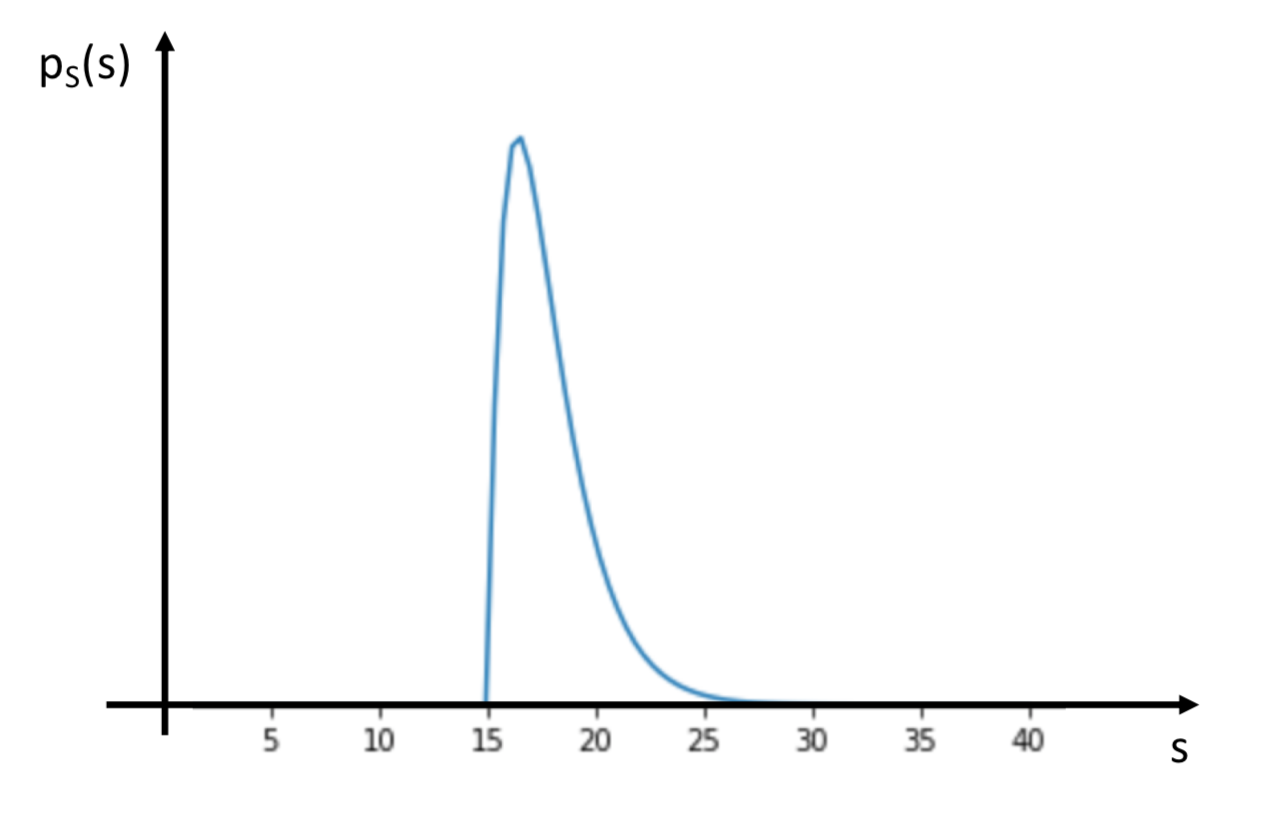
\includegraphics[scale=.25]{Figures/Fig_MC1_1.png}
\caption{Representation of the probability distribution of $S$ for $r=1$.}
\label{Fig_ps}
\end{center}
\end{figure}
\vspace{0.2cm}
\item[b)] Can we now estimate the total delivery time?\\
Let's consider that we receive an order to be delivered to one kilometer of distance ($r=1$Km), so we have that 
$$ p_S(s) = 0.7 \left(s -15\right) \exp{\left[-0.7 \left(s-15\right)  \right]}   \quad  s >15.$$
Knowing this distribution, we can know which values of $S$ are most probable and which values are completely unlikely; for instance, analyzing Figure \ref{Fig_ps}, we can realize that it is quite likely that $S$ is between $15$ and $20$, whereas it is impossible that it is lower than $15$, and it is almost impossible that it is greater than $30$. So,  in light of the distribution of $S$, we can estimate the total delivery time considering different criteria (see Figure \ref{Fig_ps_s1_s2}):

\begin{figure}[!t]
\begin{centering}
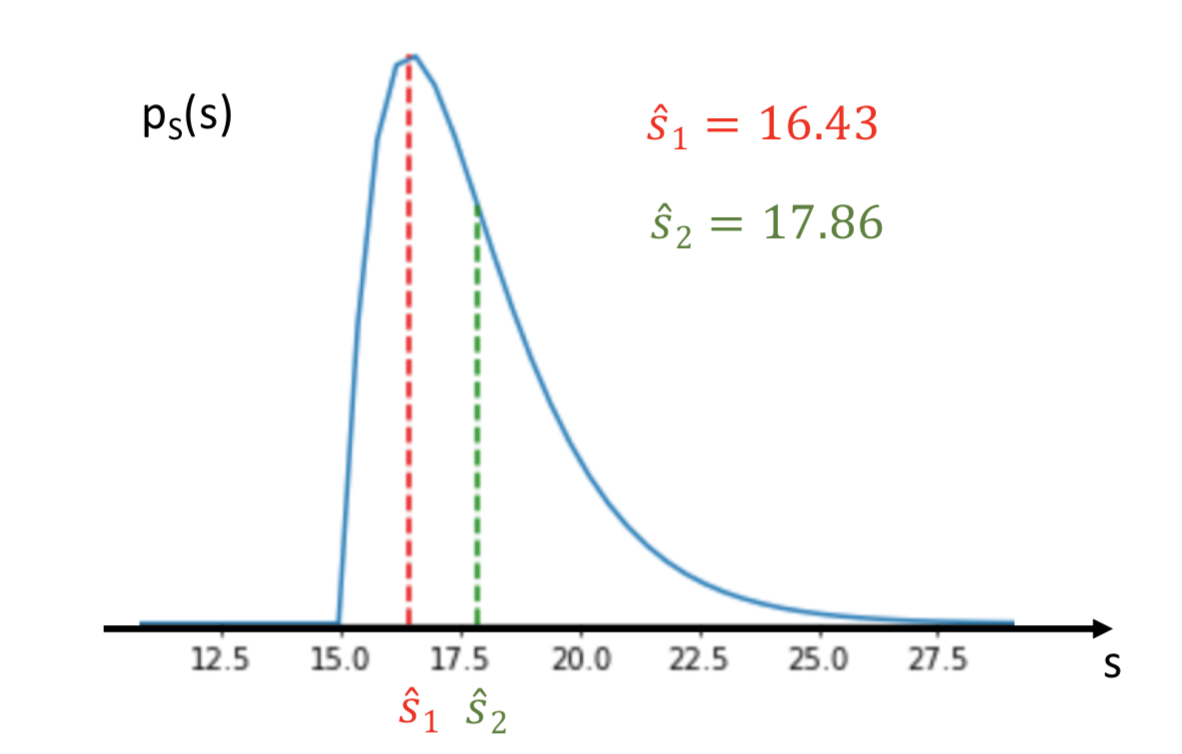
\includegraphics[scale=.25]{Figures/Fig_MC1_2.png}
\caption{Some possibles estimators of $S$ analyzing $p_S(s)$.}
\label{Fig_ps_s1_s2}
\end{centering}
\end{figure}

\begin{itemize}
\item One could consider that a good estimation could be given by the most likely value of $S$, that is, by the mode of $S$:
$$ \hat{s}_1  = {\arg\max_s}  p_S(s) $$
and we can compute this value by deriving $p_S(s)$ and setting the result to zero:

$$  \left.\frac{\partial p_S(s)}{\partial s} \right|_{s = \hat{s}_1} = 0.7 \exp{\left[-0.7 \left(\hat{s}_1 -15\right) \right]} - 0.7^2 \left(\hat{s}_1 -15\right) \exp{\left[-0.7 \left(\hat{s}_1 -15\right)  \right]} =0$$
Now, we can cancel the term\footnote{Note that by cancelling this term we are skipping the solution $\hat{s}_1 \rightarrow \infty$, but analyzing the shape of $p_S(s)$ we can check that this root is a minimum.} $0.7\exp{\left[-0.7 \left(\hat{s}_1 -15\right) \right]}$ and get:

$$ 1 - 0.7( \hat{s}_1 -15) =0$$
$$ \hat{s}_1  = 15 + \displaystyle \frac{1}{0.7}= 16.43~ {\rm min.}$$
To complete this calculation, we have to check that this solution is a maximum (the derivative only guarantees returning relative extremes or saddle points). We can do this either analyzing the shape of $p_S(s)$ or checking that the second derivative is negative.
\item Another possible estimation could be given by the expected value of $S$,
$$  \hat{s}_2 = \mathbb{E}\{S\} = \int s p_S(s) ds =  \int_{15}^{\infty} 0.7 s \left(s -15\right) \exp{\left[-0.7 \left(s-15\right)  \right]} ds $$
and solving this integral by parts, we have
$$ \hat{s}_2 =   15 + \displaystyle \frac{2}{0.7}=17.86~{\rm min.}$$
\item Or we could even raise other estimators, such as the median of the distribution or the 25\% or 75\% percentiles. 
\end{itemize}

Finally, it is important to bear in mind that regardless of the estimator we use, we probably have an estimation error (it is practically impossible for the estimated value to coincide with the actual one) and the error of each estimator will indicate us which estimator is more adequate. %In fact, if we know how our problem is going to measure the different errors (what the cost function gives us), the ideal is for us to design the estimator trying to minimize this cost. 
In fact, in this unit we will pursue as a design criterion the minimization of the mean value of a cost criterion that establishes how we should penalize different kinds of errors.

\vspace{0.2cm}
\item[c)] How can we find the optimal estimator for a given cost? 
For the design of the estimator, the food delivery company wants to minimize the following cost function (see Figure \ref{Fig_MC1_5}):
\begin{equation} 
c(\hat{s},s) = \begin{cases}
0.005|s-\hat{s}| & {\rm if} \quad \hat{s}>s\\
0.1|s-\hat{s}|  & {\rm if} \quad \hat{s}<s 
\end{cases} \nonumber
\end{equation} 

%{\color{red} Podemos dar un significado a este coste? Perdidas en Keuros? Pero en ese caso siempre pierde... y no tiene sentido definir costes negativos que serían beneficios.... Ponemos unas ganancias máximas y esto son perdidas sobre esas ganacias....???}

\begin{figure}[!t]
\begin{tabular}{m{.1\textwidth}m{.5\textwidth}m{.4\textwidth}}
&\raisebox{-18ex}{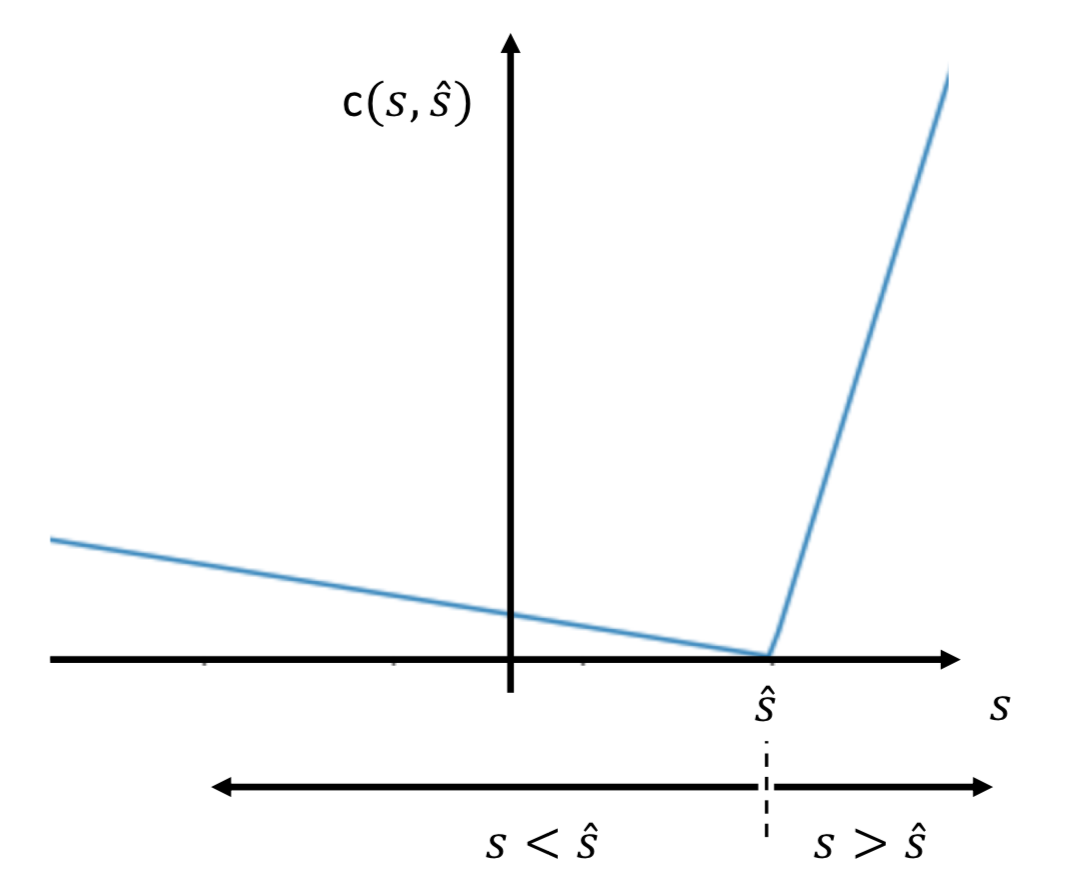
\includegraphics[scale=.25]{Figures/Fig_MC1_5.png}}&
 \begin{equation} 
c(\hat{s},s) = \begin{cases}
0.005|s-\hat{s}| & {\rm if} \quad \hat{s}>s\\
0.1|s-\hat{s}|  & {\rm if} \quad \hat{s}<s 
\end{cases} \nonumber
\end{equation} 
\end{tabular}
\caption{Asymmetric cost function to be minimized during the estimator design.}
\label{Fig_MC1_5}
\end{figure}

As any cost function, this cost function indicates how we have to penalize the fact that the estimated value differs from the actual value of $S$. However, unlike typical cost functions, this is an asymmetric cost function (see Figure \ref{Fig_MC1_5}), that is, it applies different penalties in case of overestimating the values of $S$ ($\hat{s} >s $) or underestimating them ($\hat{s} <s $). In this way, this cost function is indicating that if the order arrives before the time we have estimated it will penalize less than in case the customer has to be waiting longer than expected, i.e., if our  order takes longer to arrive than we have estimated. In this case, using the mean or median of $S$ is not the most appropriate estimator, and we should choose a value higher than the expected one. I.e., since subestimations of the actual time of delivery are highly penalized, we should try to be conservative and produce estimators that are only rarely exceeded. So, it is possible that a value around the 70\%-80\% percentile of the $p_S(s)$ distribution is close to the estimator we are looking for.


Reviewing the expression of the cost function to be minimized, we can see that the cost value depends both on the estimator $\hat{s}$ and on the random variable to be estimated $S$. So, as the cost function is a function of a random variable, it is itself another random variable. For this reason, we are going to denote it as $ C = c(\hat{s},S)$.

\begin{figure}[!t]

\begin{tabular}{m{.5\textwidth}m{.5\textwidth}}
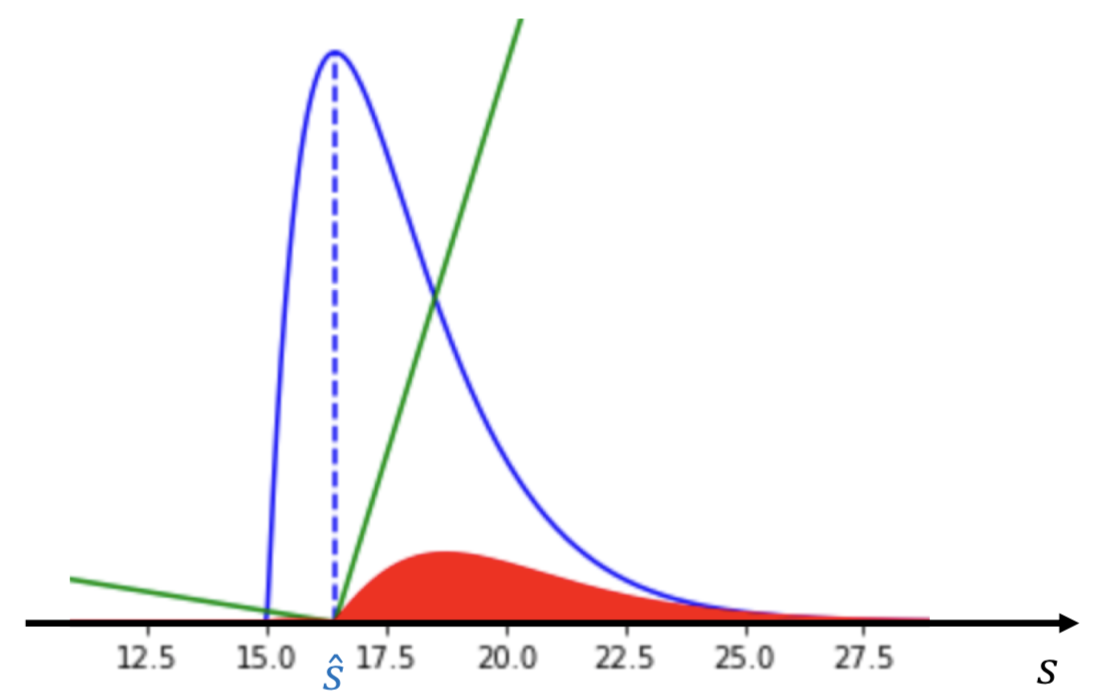
\includegraphics[scale=.3]{Figures/Fig_MC1_6.png}&
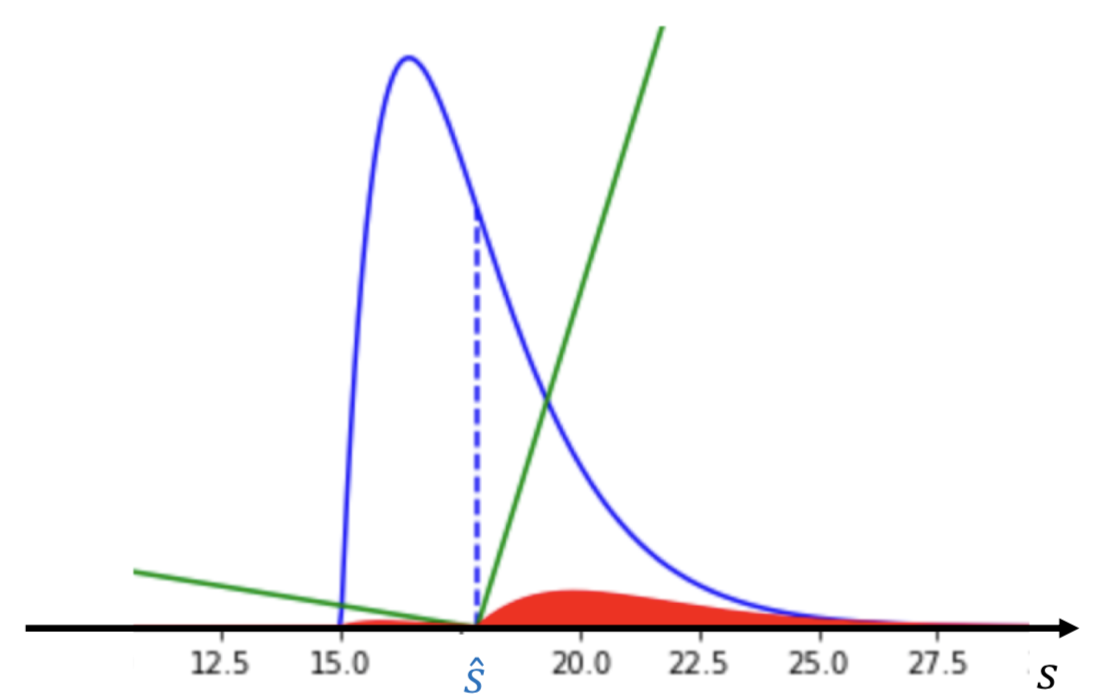
\includegraphics[scale=.3]{Figures/Fig_MC1_7.png}\\
(a) $\hat{s} = 16.43 \quad \mathbb{E}\{C\} = 0.23$ &
(b) $\hat{s} =  17.86 \quad  \mathbb{E}\{C\} = 0.12 $ \\
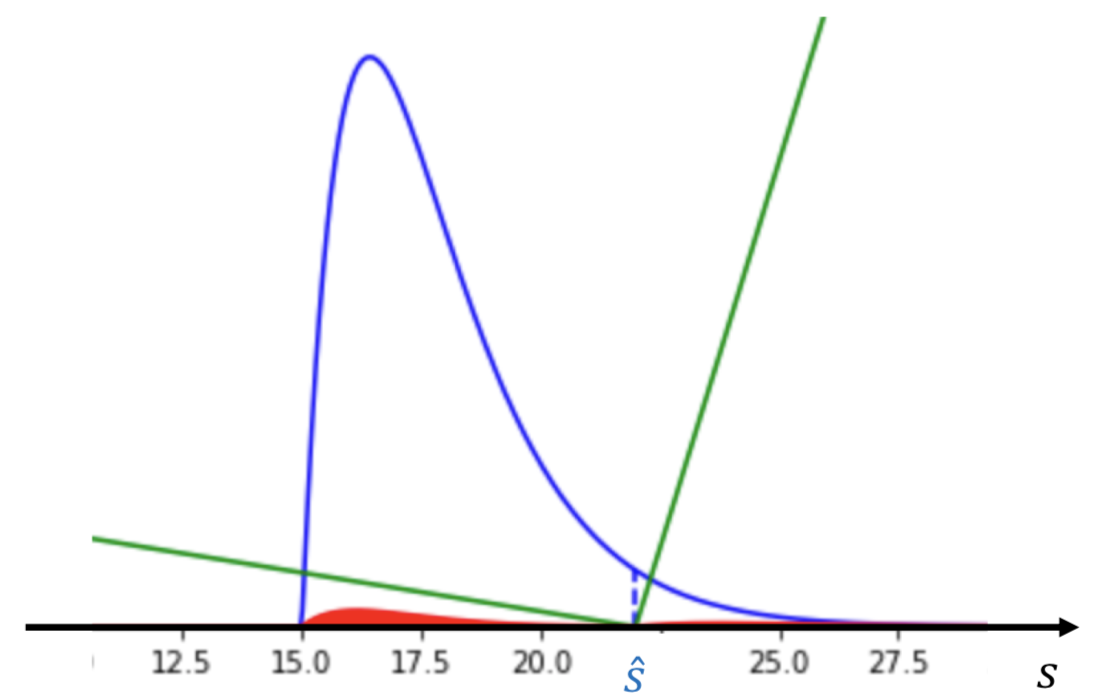
\includegraphics[scale=.3]{Figures/Fig_MC1_8.png}&
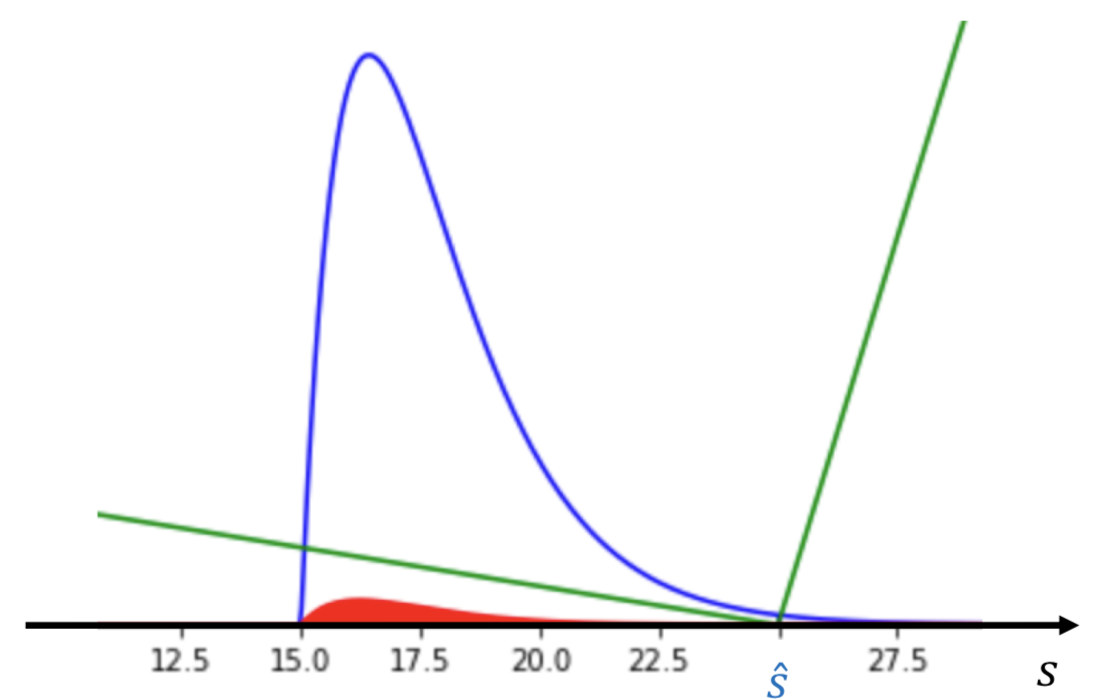
\includegraphics[scale=.3]{Figures/Fig_MC1_9.png}\\
(c) $\hat{s} = 22  \quad \mathbb{E}\{C\}= 0.04$ &
(d) $\hat{s} =  25 \quad \mathbb{E}\{C\}=0.05$ \\
\multicolumn{2}{c}{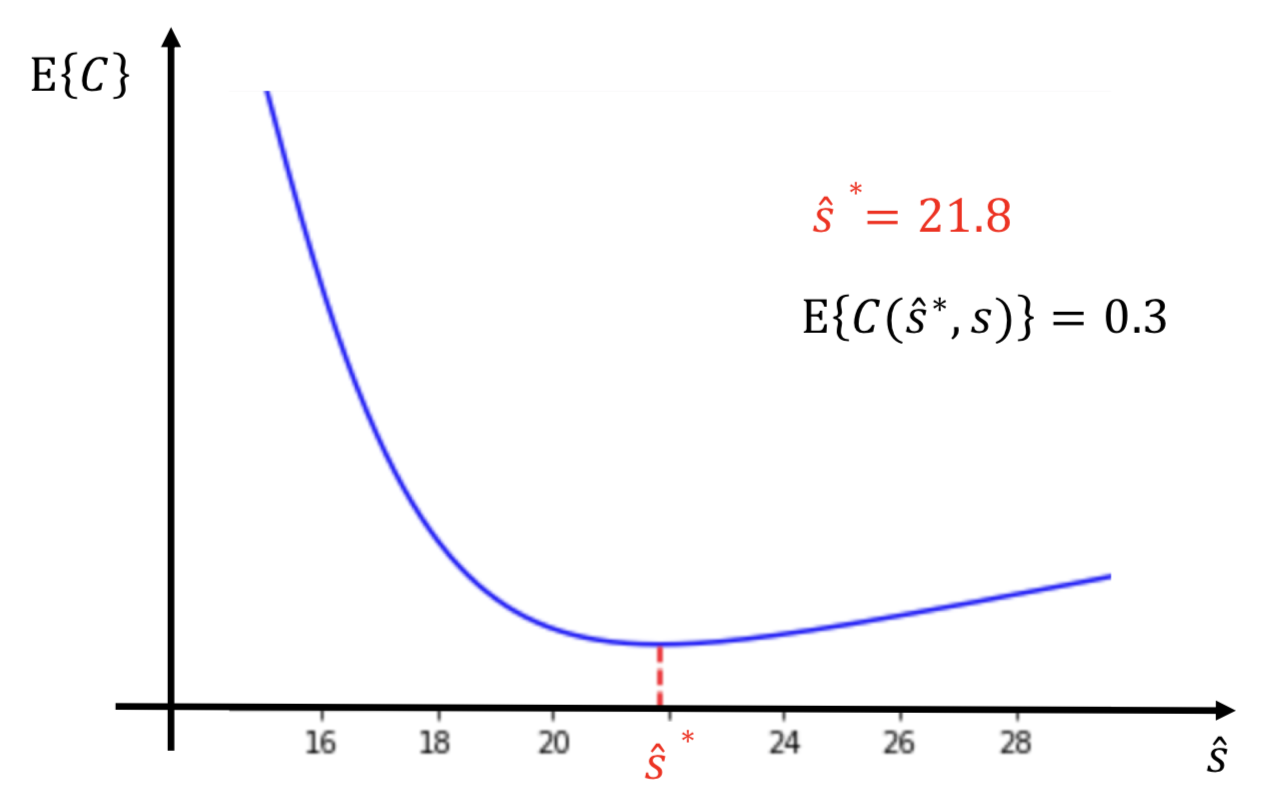
\includegraphics[scale=.25]{Figures/Fig_MC1_10.png}}\\
\multicolumn{2}{c}{(e) Evolution of the mean cost with the value of $\hat{s}$}
\end{tabular}
\caption{Process of minimization of the mean cost for different values of the estimator.}
\label{Fig_MC1_6_9}
\end{figure}

When we wanted to find the value of the estimator that minimizes the cost $C$, we would have to find the value of the estimator which minimizes the expected cost or the mean cost. So, the optimum estimator would be given by:
$$ \hat{s}^{*} = \arg\min_s~ \mathbb{E}\{C\} = \arg\min_{\hat{s}}~ \mathbb{E}\{c(\hat{s},S)\}$$
where the mean cost is computed as:
$$\mathbb{E}\{c(\hat{s},S)\} = \int c(\hat{s},s) p_s(s) ds$$


For each possible value of the estimator, we will get a different mean cost, and we will have to select the estimator value that provides the minimum mean cost. Fig \ref{Fig_MC1_6_9} shows the average cost for different values of the estimator for the given asymmetric cost function. In fact, Subfigures \ref{Fig_MC1_6_9}(a)-(d) show how the mean cost is computed for different values of the estimator; note that the mean cost is computed as the area resulting from multiplying the distribution $p_S(s)$ by the cost function $c(\hat{s},S)$, and, as different values of the estimator, $\hat{s}$,  will place the cost function in different positions, this process will result in different mean costs. If we directly compute the mean cost for any possible value of $\hat{s}$ we would obtain a curve similar to that shown in Subfigure \ref{Fig_MC1_6_9}(e) and $\hat{s}^{*}$ would be the value of $\hat{s}$ which minimizes it. In this case, we can see that the optimum  estimator would be $\hat{s}^{*} = 21.8$ min and it generates a mean cost of $0.3$.


\end{itemize}
\end{solution}

\subsection{Example 2: Bayesian estimation with observations}
\label{subsec:example2}

\begin{problem}
To obtain a more accurate estimation of the delivery time, the company has improved the food preparation process, so that it is able to know the exact time it will take to prepare the order $T_1=t_1$. 

When we want to estimate the value of $S$ without observations, the only distribution which provides information about the value of $S$ is $p_S(s)$; however, when we have additional information such as knowledge of the value of $t_1$ (observation), including this information in our estimation problem makes the estimation of $S$ easier (more accurate). Adding this knowledge (observation) to the estimation task implies using the posterior distribution of $S$, $p_{S|t_1}(s|t_1)$, instead of using $p_S(s)$.

To solve the estimation problem in this new scenario, let's try to answer the following questions:
 \begin{itemize}
\item[a)] Can we obtain the probability distribution of $S$ given the value $T_1=t_1$?
\item[b)] Can we estimate the total delivery time for a given value $T_1=t_1$? 
\item[c)] Given a cost function to be optimized, which is the optimal estimator for a given value $T_1=t_1$? 
    \end{itemize}
\end{problem}

\begin{solution}
\begin{itemize}
\item[a)] Can we obtain the probability distribution of $S$ given the value $T_1=t_1$?\\
The calculation of the posterior distribution of $S$ can be done by applying the following r.v change\footnote{Note that as we are calculating the distribution of $S$ given $T_1$, the value of $T_1$ is known ($T_1=t_1$).}:
$$S = t_1 + T_2$$
so, $p_{S|t_1}(s|t_1)$ can be obtained by shifting the distribution of $p_{T_2}(t_2)$ to the position of $t_1$, i.e.,
$$p_{S|t_1}(s|t_1)=p_{T_2}(t_2=s-t_1) =
\frac{0.2}{r} \exp{\left[-\frac{0.2}{r} (s-t_1-5)\right]} \quad \quad  s >t_1 +5$$
%\begin{figure}[!h]
%\begin{center}
%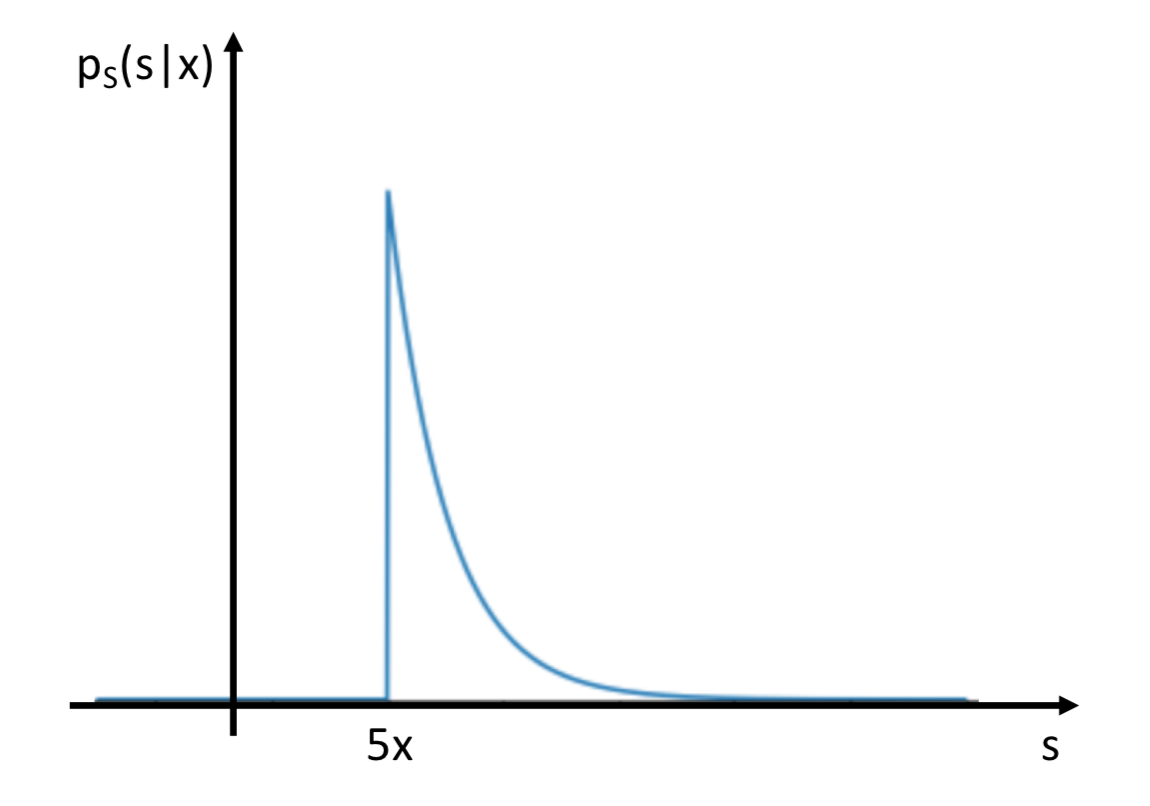
\includegraphics[scale=.25]{Figures/Fig_MC1_11.png}
%\end{center}
%\end{figure}


\item[b)] Can we estimate the total delivery time for a given value $T_1=t_1$? 

To answer this question, let's consider that a customer is calling the food company to place an order from a distance of one kilometer ($r=1$Km), and in this moment and for this order the preparation time is $t_1=12$ minutes. So we have:

$$p_{S|t_1}(s|t_1)=p_{T_2}(t_2=s-t_1) =
0.2 \exp{\left[-0.2 (s-17)\right]} \quad \quad  s >17$$

and, examining this distribution (see Figure \ref{p_S_x2}), we can consider different estimators such as the maximum of the distribution, which is $\hat{s}_1=17$ min., or the expected value of $S$ given $t_1=12$, which can be computed (by solving the integral by parts) as:

$$ \hat{s}_2= \mathbb{E}\{S|t_1=12\} = \int s p_{S|t_1}(s|t_1) ds = 17+\frac{1}{0.2} = 22 {\rm min.}$$

\begin{figure}[!t]
\begin{center}
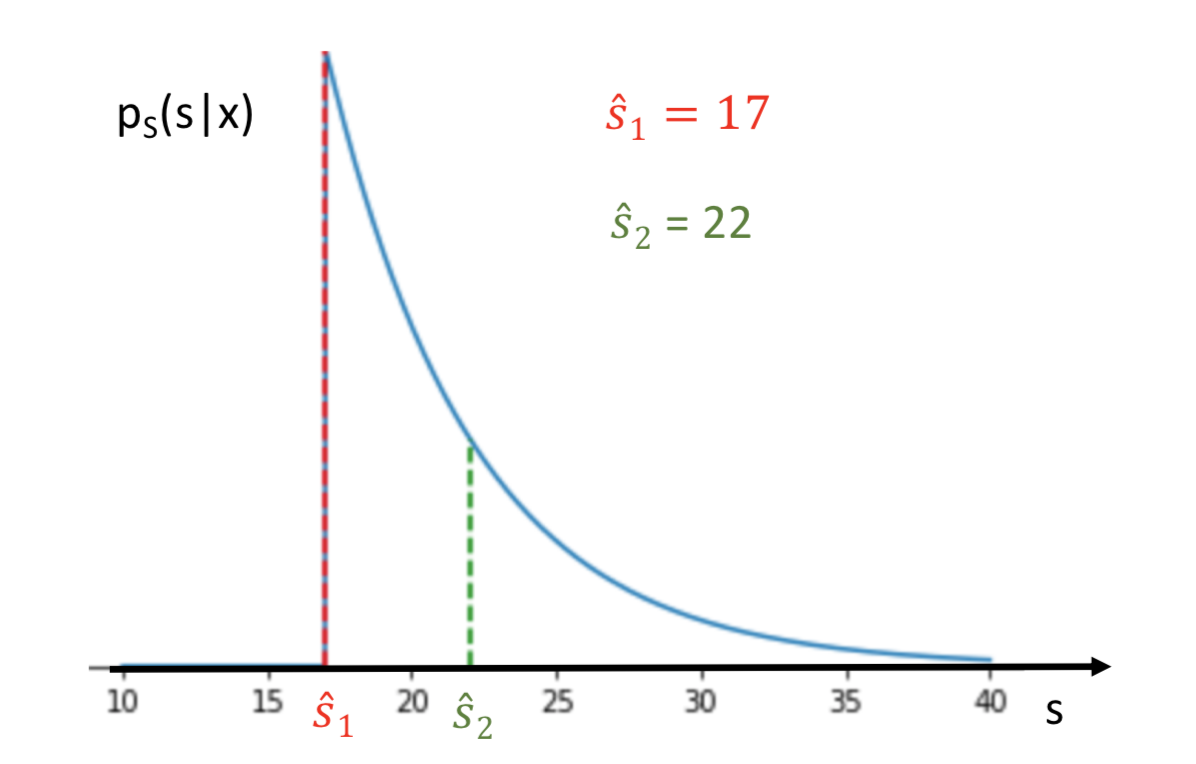
\includegraphics[scale=.25]{Figures/Fig_MC1_12.png}
\caption{Some possible estimators of $S$ given that $t_1=12$.}
\end{center}
\label{p_S_x2}
\end{figure}

For any value of the observation, the posterior distribution of $S$ will change (in this case, the $ p_{S|t_1}(s|t_1)$ will be shifted) and the value of the estimator will depend on the observation value ($t_1$). If we want to obtain a general expression for these estimators (for any value of $t_1$), we can directly compute both the maximum and the mean by using the expression of the posterior for any value of $t_1$ (we are still considering $r=1$):
$$ p_{S|t_1}(s|t_1) = 0.2 \exp{\left[-0.2 (s-t_1-5)\right]} \quad \quad  s >t_1 +5$$

For example:

\begin{itemize}
\item If we consider that the mode of $ p_{S|t_1}(s|t_1)$ could be an adequate estimator, the estimator will be:
$$ \hat{s}_1  = {\arg\max_s}  p_{S|t_1}(s|t_1) $$
In this case, as $p_{S|t_1}(s|t_1) $ is a decreasing function for $s >t_1 +5$, its maximum is 
$$\hat{s}_1 = t_1 +5.$$

\item We can also consider that the expected value of $S$ given $t_1$ is a good estimator. In this case (computing the integral by parts):
$$\hat{s}_2= \mathbb{E}\{S|t_1\} = \int s p_{S|t_1}(s|t_1) ds = 5 + t_1 +\frac{1}{0.2} = 10+t_1$$
\end{itemize}


However, in order to decide which estimator is best, we need, as before, to define which cost function we want to minimize.

\item[c)] Given a cost function to be optimized, which is the optimal estimator for a given value $T_1=t_1$? 

Again, when we are designing an estimator we may want to design it in such a way that it minimizes the mean value of a given cost function. Now, as we are now working with observations, our goal will be finding the optimal estimator for any observed value (for any given value of $T_1=t_1$). 

Thus, we can now find the optimum estimator by 
$$ \hat{s}^{*} = \arg\min_s~ \mathbb{E}\{c(\hat{s},S)|t_1\}$$
where 
$$\mathbb{E}\{c(\hat{s},S)|t_1\} = \int c(\hat{s},s) p_{S|t_1}(s|t_1)  ds$$


\begin{figure}[!t]
\begin{tabular}{m{.5\textwidth}m{.5\textwidth}}
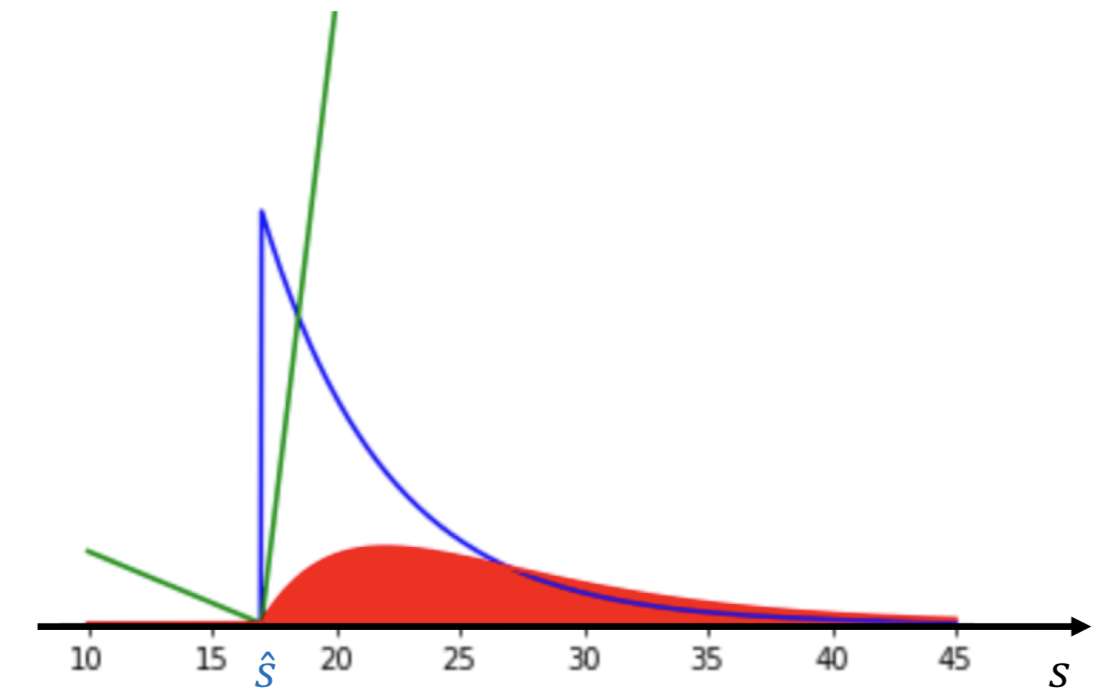
\includegraphics[scale=.3]{Figures/Fig_MC1_13.png}&
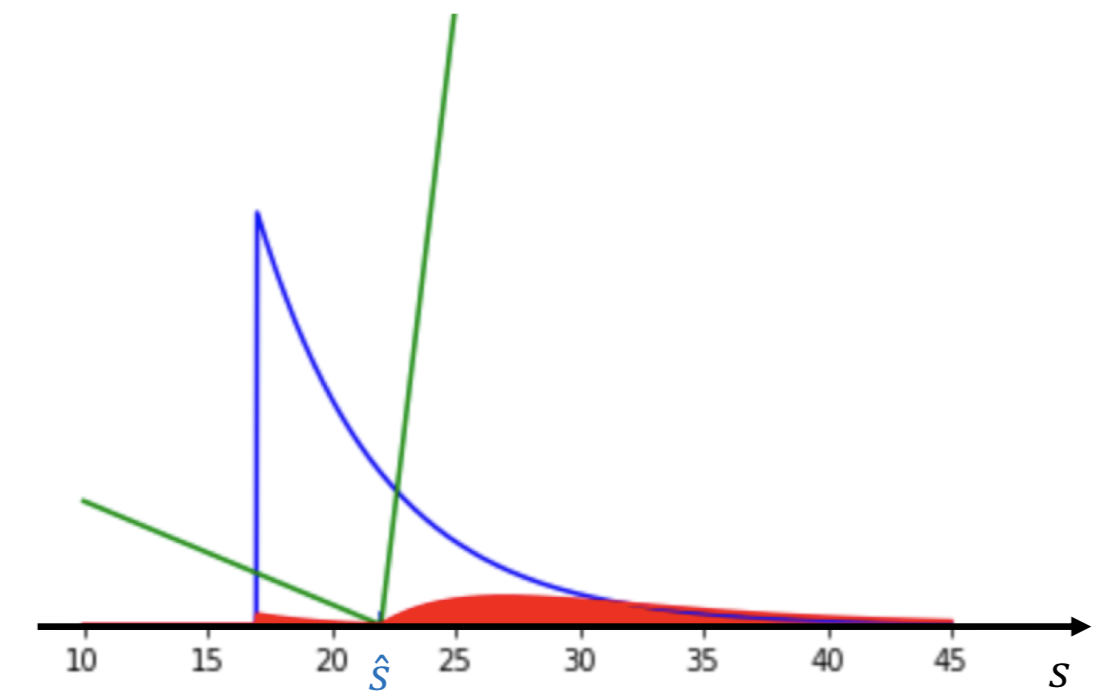
\includegraphics[scale=.3]{Figures/Fig_MC1_14.png}\\
(a) $\hat{s} = 17$ min. and  $ \mathbb{E}\{c(\hat{s},S)|x\} = 0.999$  &
(b) $\hat{s} = 12$ min. and $ \mathbb{E}\{c(\hat{s},S)|x\} = 0.385 $ \\
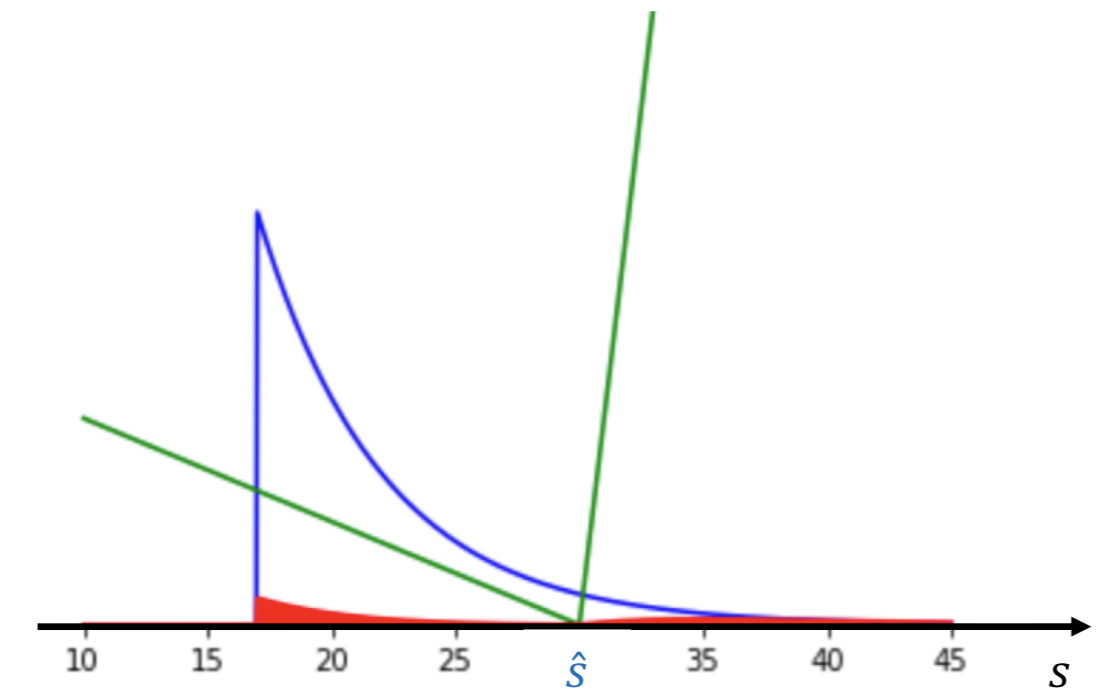
\includegraphics[scale=.3]{Figures/Fig_MC1_15.png}&
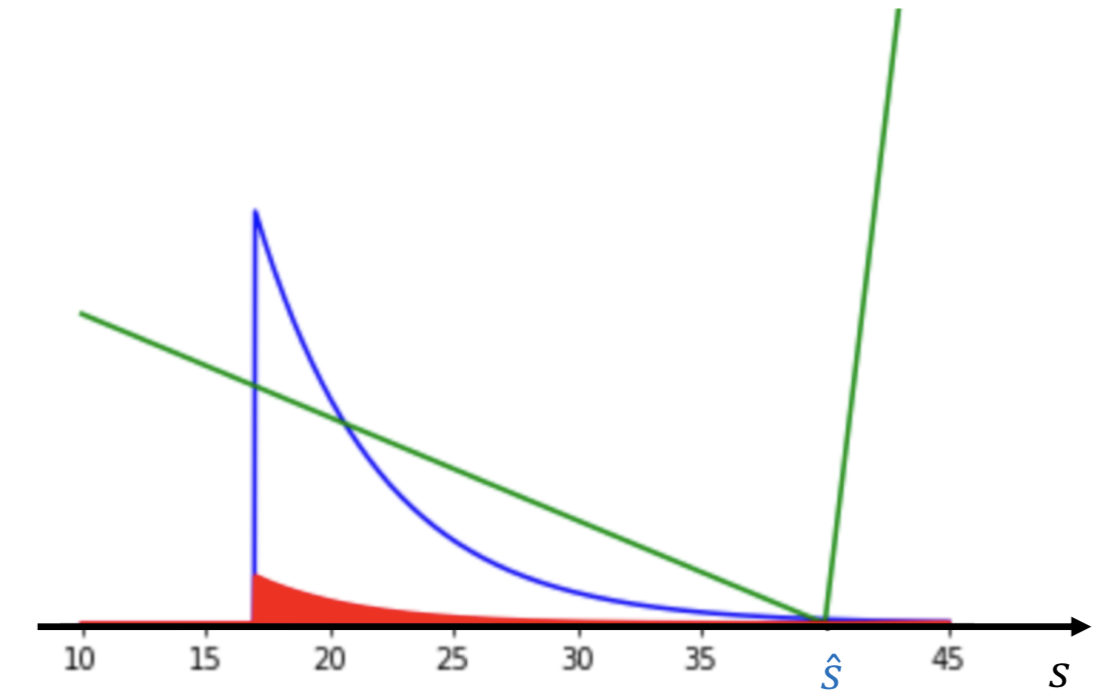
\includegraphics[scale=.3]{Figures/Fig_MC1_16.png}\\
(c) $\hat{s} = 30$ min. and  $\mathbb{E}\{c(\hat{s},S)|x\}= 0.158$ &
(d) $\hat{s} = 40$ min. and  $\mathbb{E}\{c(\hat{s},S)|x\}=0.169$ \\
\multicolumn{2}{c}{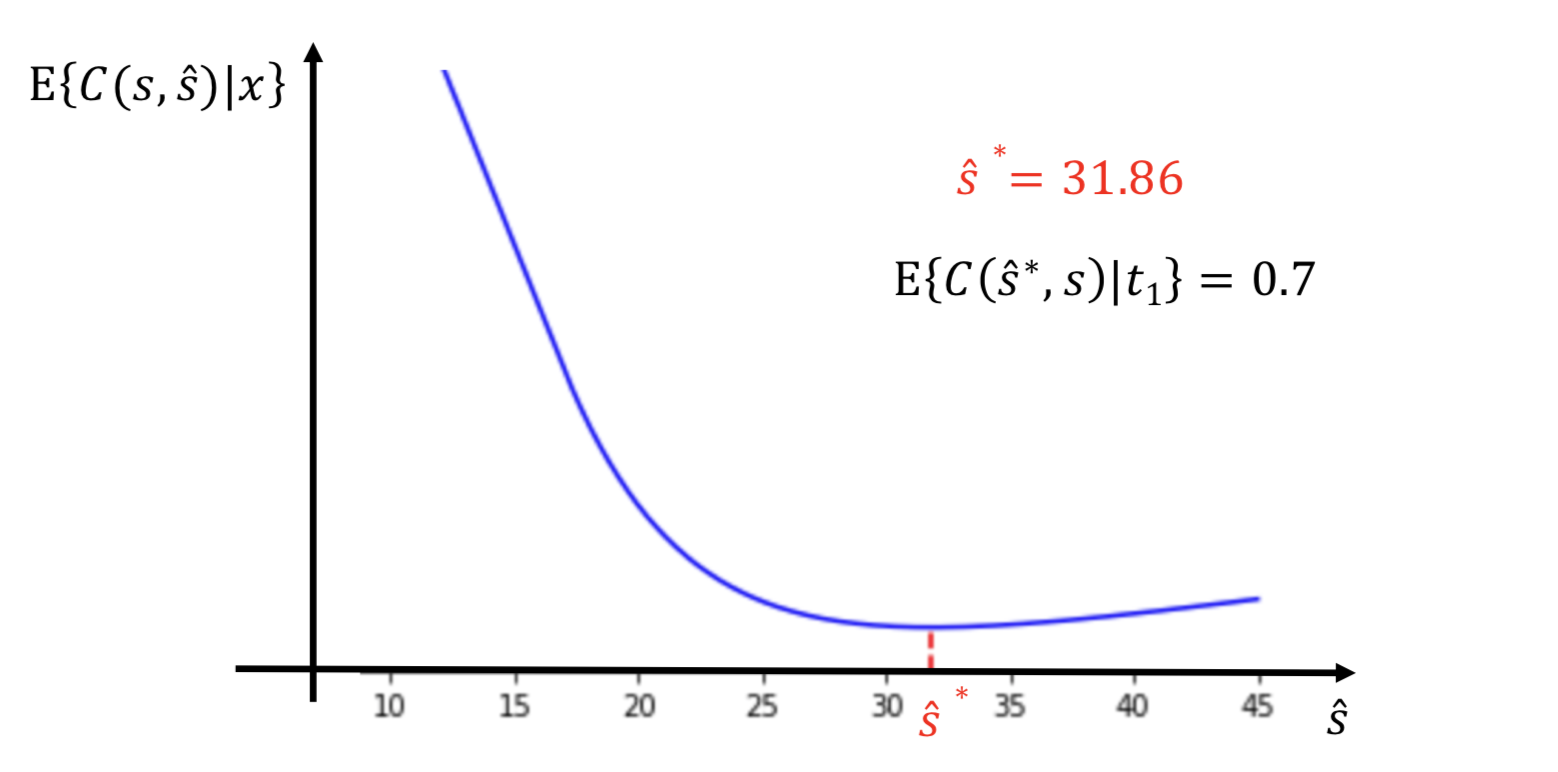
\includegraphics[scale=.25]{Figures/Fig_MC1_17.png}}\\
\multicolumn{2}{c}{(e) Evolution of the mean cost given  $t_1$ with the value of $\hat{s}$}
\end{tabular}
\caption{Process of minimization of the mean cost given $t_1$ for different values of the estimator.}
\label{Fig_MC1_13_17}
\end{figure}

Once again, each possible value of the estimator will provide a different mean cost for a given value of $t_1$ and our goal will be to select the estimator that minimizes said mean cost. 
Summarizing our example problem:
\begin{itemize}
\item An order is placed to be shipped to a distance of one kilometer ($r=1$Km);
\item For this order the preparation time is $t_1=12$ minutes;
\item We want to minimize the asymmetric cost function used in Problem \ref{subsec:example1}(c);
\end{itemize}
Fig \ref{Fig_MC1_13_17} shows the procedure of minimizing the mean cost given $t_1=12$. Subfigures \ref{Fig_MC1_13_17}(a)-(d) plot the conditional mean costs for different values of the estimator and Subfigure \ref{Fig_MC1_13_17}(e) illustrates the mean cost as a function of $\hat{s}$. Analyzing these figures, we can check that the optimum estimator value is $\hat{s}^{*} = 31.86$ min and it generates a mean cost (given that $t_1 = 12$) of $0.7$.

%{\color{red} Creo que dejar lo siguiente estarí bien si pudieramos calcular la expresión analítica de $\hat{s}^{*}$ para cualquier $t_1$ y luego el coste medio global... Como analíticamente no es sencillo, no sé si es bueno dejarlo o no.... Otra cosa es hacerlo en python y poner la gráfica o algo asi.... En cualquier caso creo que habría que incluir indicando que el estimador es una función de las observaciones y su diseño consiste en encontrar esta función...}
Finally, it is important to note that the involved mean cost is for a value of $t_1=12$. If we wanted to compare this cost with that incurred by the estimator designed without observations, we would have to compute the optimum estimator and its mean cost (given the observation) for any value of $t_1$ and average these costs taking into account the probability of each $t_1$ value. %That is, we would have to compute the global mean cost of 

%Applying this procedure, we are computing an estimator for each value of $X=x$ and minimizing the mean cost given the observation, but are we minimizing the total cost?. The answer to this question is ``yes'', since from this relationship:
%\begin{eqnarray}
%\mathbb{E}\{c(\hat{S},S)\}  & =&  \int \int c(\hat{s},s) p_{S,X}(s,x)  ds dx \nonumber \\
%&=& \int \left[ \int c(\hat{s},s) p_{S|x}(s|x)  ds \right]  p(x) dx \nonumber  \\
%&=& \int \left[ \mathbb{E}\{c(\hat{s},S)|x\}  \right]  p(x) dx \nonumber  
%\end{eqnarray}
%allows us to claim that minimizing the mean cost given the observation for any value of $x$, we are minimizing the overall mean cost.
\end{itemize}
    
\end{solution}

%\subsection{Example 3: Maximum likelihood estimation}

%\begin{problem}
%Communication channel with gaussian noise
%$$X = S +N$$


%$$p_N(n) = G(0, v_N)$$

%We transmit signal $S$ and in the receptor we observe $X$, our goal is to estimate the transmitted value ($S$) with the observation of the signal in the receptor ($X$).
%\begin{itemize}
%\item[a)] Without additional information, can we estimate the value of $S$?
%\item[b)] Could we design a bayesian estimator (the optimum estimator for a given cost)?
%\end{itemize}
%\end{problem}

%\begin{solution}
%\begin{itemize}
%\item[a)] Without additional information, can we estimate the value of $S$?
%With the given information, the only distribution that we can easily compute is the likelihood of $S$, that is, the distribution of $X$ given $S$. This distribution can be computed sifting the distribution of $N$ to the position of $S$, i.e.,

%$$p_X|s(x|s)= p_N(n= x-s) = G(s, v_N)$$

%INCLUIR FIGURA LIKELIHOOD


%This distribution indicates the probability of observing $X=x$ for a transmitted value of $S=s$. Imagine that our observation is $x=1$, then, we could use the likelihood to calculate the probability of observing $x=1$ for any value of $s$

%INCLUIR FIGURA LIKELIHOOD en funcion de s para x=1.

%At the light of this figure, what value $S$ has been transmitted? We can say 

%\item[b)] Could we design a bayesian estimator (the optimum estimator for a given cost)?
%\end{itemize}
%\end{solution}  % Input instead of include to avoid newpage after the title
\section{Statistical Estimation Theory}
\label{sec:SDT}

Once we have faced some of the main concepts involved in estimation problems, we are ready to formalize the problem for a general case.

\subsection{General view of the estimation problem}
\label{subsec:hypotheses_problems}

The design of an estimator consists of constructing a real function that, from the value of certain observation variables, provides predictions about an objective variable (or vector). 

For a general case, we will denote that random variable to be estimated as $S$ which can take any real value. As indicated in Fig. \ref{fig:est_overview}, we assume also that we have access to an observation vector $\bf x$ that can be considered as the realization of a random variable $\bf X$ lying in observation space $\cal X$. Note also that for the estimation task of $s$ or $S$ from $\bf X$ to make sense, there must be some statistical relationship between them.

\begin{figure}
\begin{center}
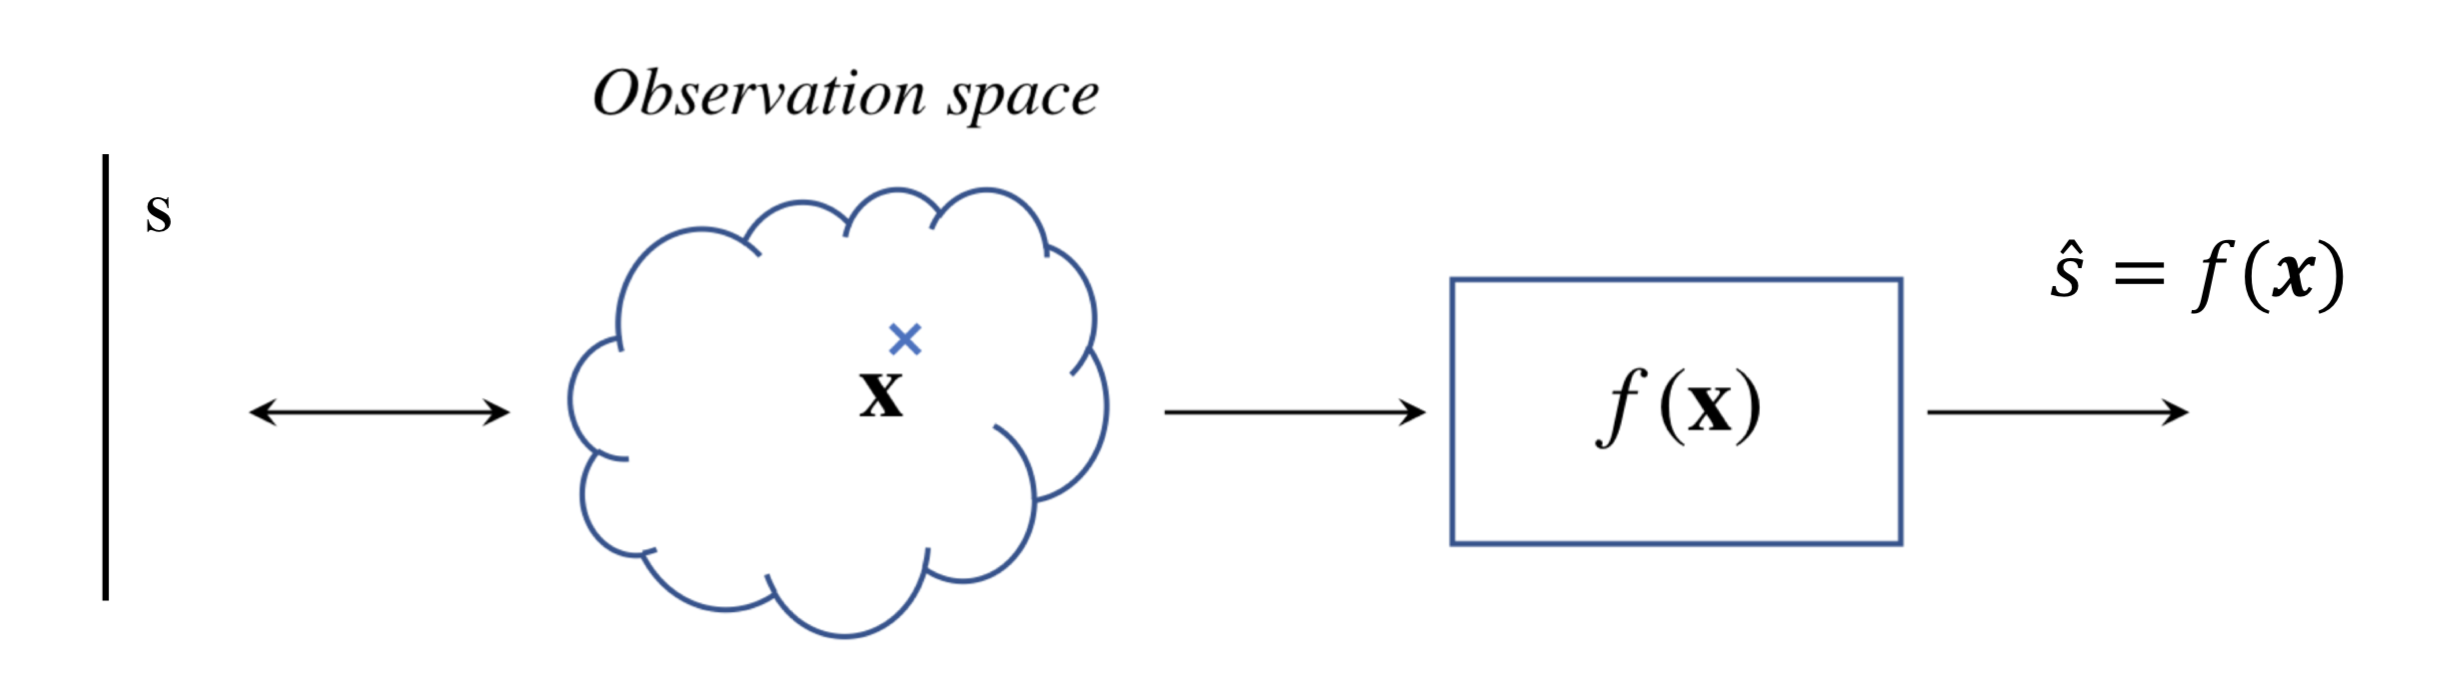
\includegraphics[width=10cm]{Figures//estimation_overview.png}
\end{center}
\caption{Diagram block of estimation problems.\label{fig:est_overview}}
\end{figure}


The estimation module implements a real output function, $\hat{S} = f({\bf X})$, $f(\cdot)$ being the estimation function. It is common to refer to this function simply as {\em estimator}, and to its output as {\em estimation}. A fundamental characteristic of the estimator is the deterministic character of the $f(\cdot)$ function, that is, for a given value $\bf x$ the estimator will always provide the same output. Note that, even though $f(\cdot)$ is deterministic, its output can be modeled as a random variable if we consider the input to the function is random vector $\bf X$.

 Since the estimator is expected to make a certain error in each application, a certain cost  (or, alternatively, a profit) will be entailed. An optimum design of our estimator must take into account this cost during the design minimizing (or maximizing) its mean value.


We consider two different kinds of problems involving estimation problems:
\begin{itemize}
    \item Analysis of estimators: Here, an estimator is given, and our purpose is to analyze its performance with respect to certain performance measure (cost function).
    \item Design of estimators: The goal is to build a function $f(\bf x)$ to optimize a given objective.
\end{itemize}

\subsection{Statistical information involved in estimation problems}
\label{subsec:statistical_info}

Before approaching the design of the estimators themselves, we collect in this subsection the different probability functions that statistically characterize the existing relationship between observations and the variable to be estimated:

%%%%%%%%%%%%%%%
\begin{itemize}
\item First, the {\bf likelihood} of the  variable $S$ is given by $p_{{\bf X}|S}({\bf x}|s)$, and statistically characterizes the generation of observations for each specific value of the variable to be estimated.
\item {\bf Posterior distribution} of $S$: $p_{S|{\bf X}}(s|{\bf x})$. It indicates which $S$ values are more or less likely to concentrate for each particular value in the observation vector.
%In the case where the variable to be estimated is deterministic, it does not make sense to condition the probability distribution of the observations to the value of $s$, so the strictly correct thing would be to denote the probability density of the observations simply as $p_{\bf X}({\bf x})$. However, note that for the estimation problem to make sense, the probability density of ${\bf X}$ has to be different depending on the real value of the deterministic parameter. For this reason, we will sometimes abuse notation and denote that dependence on observations with $s$ as $p_{{\bf X}|s}({\bf x}|s)$, referring to that probability density as the plausibility of $s$.
\item {\bf Marginal or a priori} distribution of $S$: $p_S(s)$
\item {\bf Joint distribution} of ${\bf X}$ and $S$: $p_{{\bf X},S}({\bf x},s) = p_{{\bf X}|S}({\bf x}|s) p_S(s)$. It provides the most complete statistical modeling of the joint behavior of $\bf X$ and $S$.

\end{itemize} 

%%%%%%%%%%%%%

It is important to note that the information available for estimator design may be different in each specific situation. A typical situation, because it is related to the physical process of generating the observations, is the one in which likelihood and the marginal distribution of $S$ are available. Note that from them the calculation of the joint distribution is immediate and the posterior distribution $p_{S|{\bf X}}(s|{\bf x})$ can be calculated by means of Bayes' Theorem. Remember that Bayes' Theorem allows us to obtain the posterior distribution from the {\em a priori} distribution of $S$ and its likelihood:
\begin{equation}
p_{S|{\bf X}}(s|{\bf x}) = \frac{p_{{\bf X},S}({\bf x},s)} {p_{\bf X}({\bf x})} = \frac{p_{{\bf X}|S}({\bf x}|s) p_S(s)}{\int p_{{\bf X}|S}({\bf x}|s) p_S(s) ds}
\end{equation}


\subsection{Cost functions for estimation problems}
\label{subsec_funcion_coste}


The evaluation and design of an estimator requires some objective criteria. In our case, we will consider that this criterion can materialize in the form of some function whose value we seek to maximize or minimize. %We note, however, that there are design strategies that fall outside of this approach, such as the direct maximization of some probability function.

Given that the cost function is associated with a penalty whose origin is in the discrepancy between the actual and the estimated value of $S$, it is common to accept that $c(s,\hat s) \geq 0$, verifying equality when $s = \hat s$. Alternatively, a profit function can be defined whose average value is to be maximized. In addition, it is frequent that the cost function does not depend on the specific values of $s$ and $\hat s$, but on the estimation error that is defined as the difference between the two, $e = s - \hat s$, in which case we have $c(s,\hat s) = c(s - \hat s) = c(e)$.

As an example, some frequently used cost functions are:
\begin{itemize}
\item Quadratic cost: $c(e) = e^2$.
\item Absolute value of the error: $c(e) = |e|$.
\item Relative quadratic error: $c(s,\hat s) = \frac{(s-\hat{s})^2}{s^2}$
\item Crossed Entropy: $c(s,\hat s) = - s \ln \hat s - (1-s) \ln (1-\hat s)$, for $s,\hat{s}\in [0,1]$
\end{itemize}

Accepting that this function\footnote{Note that the cost function is denoted with a $c$ minuscule because it is a deterministic function, i.e., for fixed values of $s$ and $\hat s$ the cost always takes the same value. However, as with the estimation function, the application of that function to random variables will result in another random variable, i.e., $C = c(S,\hat S)$.}  is $c(S,\hat S)$, the evaluation of an estimator is carried out by evaluating the mean value of this cost and the estimator design criterion usually involves the minimization of its mean value; i.e, this cost is used in a statistical sense, evaluating/minimizing its mean value, which is equivalent to evaluating/minimizing the average cost that would be obtained by performing an infinitely large number of experiments.

In general, the mean cost of an estimator is given by
\begin{align}
\label{Est:coste_medio_gen}
\mathbb{E}\{c(S,\hat S)\} 
    & = \int_{\bf x} \int_s c(s,\hat s) p_{S,{\bf X}}(s,{\bf x}) ds d{\bf x}
\end{align}
where it should be noted that $\hat{s}$ is generally a function of ${\bf x}$.




{
%%%%%%%%%%%%%%%
\begin{example}[Evaluation of estimators 1]
\label{CalculoECM}
Suppose that the joint distribution of $S$ and $X$ is given by
\begin{equation}
p_{S,X}(s,x) = \left[
\begin{array}{ll}
\frac{1}{x}, & \qquad 0<s<x ~~{\rm and}~0<x<1 \\
0,           & \qquad \text{otherwise}
\end{array}
\right.
\end{equation}
Let's consider two estimators $\hat{S}_1 = \frac{1}{2}X$ and $\hat{S}_2 = X$. \textquestiondown Which is the best estimator from the point of view of the quadratic cost? To find out, we'll calculate the mean quadratic error for both estimators.
Knowing that, for any $w$,
\begin{align}
\mathbb{E}\{(S-wX)^2\}   
 &= \int_0^1 \int_0^x (s-wx)^2 p_{S,X}(s,x) ds dx   \nonumber\\
 &= \int_0^1 \int_0^x (s-wx)^2 \frac{1}{x}ds dx   \nonumber\\
 &= \int_0^1 \left(\frac{1}{3} - w  + w^2 \right) x^2 dx  \nonumber\\
 &= \frac{1}{3}\left(\frac{1}{3} - w  + w^2 \right) 
\end{align}
Taking $w=1/2$ results in
\begin{align}
\mathbb{E}\{(S-\hat{S}_1)^2\} & = \mathbb{E}\{(S-\frac{1}{2}X)^2\}   
 = \frac{1}{3}\left(\frac{1}{3} - \frac{1}{2}  + \frac{1}{4} \right) = \frac{1}{36}
\end{align}
Alternatively, by taking $w=1$ we get
\begin{align}
\mathbb{E}\{(S-\hat{S}_2)^2\} & = \mathbb{E}\{(S-X)^2\}   
 = \frac{1}{3}\left(\frac{1}{3} - 1  + 1 \right) = \frac{1}{9}
\end{align}
Therefore, from the point of view of the quadratic mean error, $\hat{S}_1$ is a better estimator than $\hat{S}_2$.
\end{example}\vspace{0.4cm}}
%%%%%%%%%%%%%


\begin{example}[Evaluation of estimators 2]
Consider that $X$ is a noisy observation of $S$, so that
\begin{equation}
X = S + R
\end{equation}

where $S$ is a random variable of mean 0 and variance 1, and $R$ is a random Gaussian variable, independent of $S$, of mean $0$ variance $v$. Considering the estimator $\hat{S} = X$, obtain the associated  mean quadratic cost and mean absolute error.

The mean quadratic cost is given by:

\begin{equation}
\mathbb{E}\{(S-\hat{S})^2\} = \mathbb{E}\{(S-X)^2\} = \mathbb{E}\{R^2\} = v
\end{equation}
And the mean absolute error
\begin{align}
\mathbb{E}\{|S-\hat{S}|\}
    &= \mathbb{E}\{|R|\} 
     = \int_{-\infty}^{\infty} |r| \frac{1}{\sqrt{2\pi v}}\exp\left(-\frac{r^2}{2v}\right)dr 
\nonumber\\
    &= 2 \int_{0}^{\infty} r \frac{1}{\sqrt{2\pi v}}\exp\left(-\frac{r^2}{2v}\right)dr 
     = \sqrt{\frac{2v}{\pi}}
\end{align}
\end{example}\vspace{0.4cm}
\section{Design of estimators}

\subsection{ML and MAP estimators}

We define the maximum likelihood estimator (ML) as
\begin{equation}
\hat s_{\text{ML}} = \arg\max_{s} p_{{\bf X}|S}({\bf x}|s)
                   = \arg\max_{s} \ln(p_{{\bf X}|S}({\bf x}|s))
                    \label{ec:est_ML}
\end{equation}

It is important to emphasize that the maximization of $p_{{\bf X}|S}({\bf x}|s)$ has to be done with respect to the value of $s$, which is not the variable for which this probability function is defined. %Note that in the estimator definition alternatively includes  the use of the logarithm function (or some other with similar properties) and its use does not affect in any case the value resulting from maximization.

On the other hand, we define the maximum a posterior estimator (MAP) as
\begin{equation}
\hat s_{\text{MAP}} = \arg\max_{s} p_{{S|\bf X}}(s|{\bf x})
                   = \arg\max_{s} \ln(p_{{S|\bf X}}(s|{\bf x}))
                   \label{ec:est_MAP}
\end{equation}

in this case, maximization is performed on the same variable of the distribution that is being maximized. 

Note that both \eqref{ec:est_ML} and \eqref{ec:est_MAP} alternatively include the use of the logarithm function. This is done by practical reasons, since for the maximization of either the likelihood or the posterior of $S$ it may be useful to introduce an auxiliary function that simplifies the analytical form of the function and, since the logarithm function is defined for every positive value of its argument and is strictly increasing, it implies that if $p_{S|{\bf X}}(s_1|{\bf x}) > p_{S|{\bf X}}(s_2|{\bf x})$, then also $\ln p_{S|{\bf X}}(s_1|{\bf x}) > \ln p_{S|{\bf X}}(s_2|{\bf x})$). So, the introduction of the logarithm function will be useful when the likelihood or the a posterior  present products or exponentials, as it will transform products into sums and it will cancel exponentials. In this way, the maximization process can be simplified considerably.

If we compare both estimators, the ML estimator uses as statistical the likelihood of $S$ (a distribution which models the generation of the observations), whereas the MAP estimator uses the posterior distribution of $S$ (characterizes the behaviour of $S$ for any observed value), so the MAP estimator has a more complete information of the variable to be estimated. Nevertheless, the ML estimation does not require the definition of probability densities on the variable to be estimated (a prior or posterior distribution of the $S$ are not needed). Therefore, the use of the ML estimator is often used (or it is more appropriated) when such information is not available.

The ML estimator coincides with the MAP when $S$ has a uniform distribution in a range of values and, therefore, the application of the ML estimator in the absence of information about the a prior distribution of $S$ is equivalent to assuming uniformity in $S$ and applying the MAP estimator. To check this equivalence, one need only consider the relationship between the likelihood and the posterior distribution of $S$ by means of the Bayes Theorem,
$$ \hat s_{\text{MAP}} = \arg\max_{s} p_{{S|\bf X}}(s|{\bf x}) =  \arg\max_{s} \frac{p_{{\bf X}|S}({\bf x}|s) p_S(s)} {p_{\bf X}({\bf x})} $$
Since $p_{\bf X}({\bf x})$ does not depend {on $s$} and we are assuming that $p_S(s)$ is constant, we get:
$$ \hat s_{\text{MAP}} = \arg\max_{s} p_{{\bf X}|S}({\bf x}|s) = \hat s_{\text{ML}}$$
That is, the value of $s$ that maximizes the posterior has to coincide with the one that maximizes likelihood.



%%%%%%%%%%%%%%%
\begin{example}[Estimation ML]
\label{ex:est_ML_varaleat}
We want to estimate the value of a random variable $S$ from an observation $X$ statistically related to it. For the design of the estimator, only the likelihood of $S$ is known, which is given by
\begin{equation}
p_{X|S}(x|s) = \frac{2 x}{(1 - s)^2},\;\; 0<x<1-s,\;\; 0<s<1
\end{equation}
Given the available statistical information, it is decided to construct the ML estimator of $S$. For this purpose, the previous likelihood should be maximized. Such likelihood is a probability density function of $X$ as represented in Figure \ref{fig:est_ML_caso1}(a), where it is verified that the integral of this function with respect to $x$ is unitary. However, to carry out the maximization that allows to find $\hat s_{\text ML}$ it is more useful to represent this likelihood as a function of $s$ (Fig.\ref{fig:est_ML_caso1}(b))\footnote{Note that the integral with respect to $s$ of $p_{X|S}(x|s)$ will not generally be the unit, since this function does not constitute a probability density of $S$.}. From this graphic representation it is evident that the estimator is
$$\hat s_{\text{ML}} = 1 - x$$
or, alternatively, if we consider the application of the estimation function on the random variable $X$ instead of on a specific value of it,
$$\hat S_{\text{ML}} = 1 - X$$

%%%%%%%%%%%%%%
\begin{figure}[t]
  \begin{center}
  \begin{tabular}{cc}
    %\epsfig{file=Figures/px_s_funcionx, width=6cm} 
    \includegraphics[width=6cm]{Figures//px_s_funcionx.png} &
   % \epsfig{file=Figures/px_s_funcions, width=6cm} \\ 
   
   \includegraphics[width=6cm]{Figures//px_s_funcions.png}\\
    (a) & (b)
  \end{tabular}
    \caption{Representation of the likelihood distribution of the exercise \ref{ex:est_ML_varaleat} as a function of $x$ and $s$.}
    \label{fig:est_ML_caso1}
  \end{center}
\end{figure}
%%%%%%%%%%%%

\end{example}\vspace{0.4cm}
%%%%%%%%%%%%%


{
%%%%%%%%%%%%%%%
\begin{example}[Estimation MAP]
Considering that  
\begin{equation}
p(s|x) = \frac{1}{x^2} s \exp\left(-\frac{s}{x}\right), \qquad  x\ge 0, s \ge 0
\end{equation}
The MAP estimator can be computed maximizing
\begin{equation}
\ln(p(s|x)) = -2\ln(x) + \ln(s)-\frac{s}{x}, \qquad  x\ge 0, s \ge 0
\end{equation}
Since $\l(p(s|x))$ tends to $-\infty$ around $s=0 $ and $s=\infty$, its maximum must be at some intermediate point with zero derivative. Deriving respect to $s$ results in
\begin{equation}
\left.\frac{\partial}{\partial s} \ln p(s|x)\right|_{s=\hat{s}_\text{MAP}} = \frac{1}{\hat{s}_\text{MAP}} - \frac{1}{x} = 0, \qquad  x\ge 0, s \ge 0
\end{equation}
Thus,
\begin{equation}
\hat{s}_\text{MAP} = x
\end{equation}
\end{example}\vspace{0.4cm}}
%%%%%%%%%%%%%


\subsection{Bayesian design of estimators}

It is worth asking, for a given cost and distribution, which is the best possible estimator. We can find this out by taking into account that, generally speaking, the average cost can be expressed as
\begin{align}
\label{ec:coste_medio}
\mathbb{E}\{c(S,\hat S)\} 
& = \int_{\bf x} \int_s c(s,\hat s) p_{S|{\bf X}}(s|{\bf x}) ds\;p_{\bf X}(\bf x) d{\bf x} = \nonumber\\
& = \int_{\bf x} \mathbb{E}\{c(S,\hat s)|{\bf X} = {\bf x} \} p_{\bf X}(\bf x) d{\bf x}.
\end{align}

The last line of this equation shows that a strategy for minimizing the overall estimation cost consists of minimizing the mean cost for each possible value of the observation vector,  $\mathbb{E}\{c(S,\hat s)|{\bf X} = {\bf x} \}$, which we will refer to as mean posterior cost or mean cost given ${\bf X}$. Therefore, both strategies (minimization of the expected cost for all $S$ and $\bf X$, or conditioned to the value of $\bf X$) are in principle equivalent in order to obtain the optimal estimator associated with a given cost function.

The Bayesian Estimator associated with a cost function is defined {as} that which minimizes \eqref{ec:coste_medio}, that is:

\begin{equation}
\label{ec:est_bayesiano}
{\hat s}^* = \arg\min_{\hat s}\;\mathbb{E}\{c(S,\hat s)|{\bf X} = {\bf x} \}
\end{equation}

where $\hat s^*$ is the Bayesian Estimator. According to our previous discussion, the Bayesian Estimator also minimizes the expected cost in a global sense, i.e., for all $S$ and ${\bf X}$. Note, however, that for your design the expression \eqref{ec:est_bayesiano} is more useful than the direct minimization of the overall cost.

\begin{equation}
\mathbb{E}\{c(S,\hat S)\} = \int_{\bf x} \mathbb{E}\{c(S,\hat s)|{\bf X} = {\bf x} \} p_{\bf X}(\bf x) d{\bf x}
\end{equation}

since calculating the integral in ${\bf x}$ would require knowing beforehand the relationship between $\hat s$ and $\bf x$, which is precisely the objective of the estimator design problem.

%%%%%%%%%%%%%%%
\begin{example}[Calculation of a minimum mean square error estimator]
\label{CalculoECM2}
Following the example \ref{CalculoECM}, we can calculate the posterior distribution of $S$ through
\begin{equation}
p_{S|X}(s|x) = \frac{p_{S,X}(s,x)}{p_{X}(x)}. 
\end{equation}
Knowing that
\begin{equation}
p_{X}(x) = \int_0^1 p_{S,X}(s,x) ds = \int_0^x \frac{1}{x} ds = 1,
\end{equation}
we obtain
\begin{equation}
p_{S|X}(s|x) = \left[
\begin{array}{ll}
\frac{1}{x}, & \qquad 0<s<x<1 \\
0,           & \qquad \text{otherwise}
\end{array}
\right.
\end{equation}
The mean cost given the observation will be given by
\begin{align}
\mathbb{E}\{c(S,\hat s)|X=x\} 
   &= \mathbb{E}\{(S-\hat s)^2|X=x\} \nonumber\\
   &= \int_0^1 (s-\hat{s})^2 p_{S|X}(s|x) ds   \nonumber\\
   &= \frac{1}{x} \int_0^x (s-\hat{s})^2 ds   \nonumber\\
   &= \frac{1}{x} \left(\frac{(x-\hat{s})^3}{3} + \frac{\hat{s}^3}{3} \right)    \nonumber\\
   &= \frac{1}{3}x^2 - \hat{s} x + \hat{s}^2. 
\label{Est:ECMsx}
\end{align}

As a function of $\hat{s}$, the mean cost conditioned to the observation is a polynomial of second degree, whose minimum can be calculated immediately by derivation. Being
\begin{align}
\frac{d}{d\hat{s}} \mathbb{E}\{c(S,\hat s)|X=x\} 
   &= - x + 2 \hat{s} ,
\end{align}
the lowest mean quadratic error estimator will be
\begin{equation}
\label{eq:sopt_halfx}
\hat{s}^* = \frac{1}{2}x,
\end{equation}
which matches the estimator $\hat{S}_1$ from the example \ref{CalculoECM}. Therefore, $\hat{S}_1$ is the best possible estimator from the point of view of the mean square error.
\end{example}\vspace{0.4cm}
%%%%%%%%%%%%%

Based on \eqref{ec:est_bayesiano} we can conclude that, regardless of the cost to be minimized, the knowledge of the posterior distribution of $S$ given ${\bf X}$, $p_{S|{\bf X}}(s|{\bf x})$, is sufficient for the design of the Bayesian Optimal Estimator. As mentioned above, this distribution is often calculated from the likelihood of $S$ and its a prior distribution using the Bayes Theorem, which is in fact the origin of the denomination of these estimators.

%%%%%%%%%%%%%%%%%%%%%%%%%%%%%%%%%%%%%%%%%%%%%%%%%
\section{Common bayesian estimators}
%%%%%%%%%%%%%%%%%%%%%%%%%%%%%%%%%%%%%%%%%%%%%%%%%

This section presents some of the most commonly used Bayesian estimators. For their calculation, we will proceed to minimize the mean cost given $\bf X$ (posterior mean cost) for different cost functions.


%%%%%%%%%%%%%%%%%%%%%%%%%%%%%%%%%%%%%%%%%%%%%%%%%%%%%%%%%%%%%%
\subsection{Minimum Mean Squared Error estimator (MSE)}
The estimator of minimum mean squared error (MSE) is the one associated with the cost function $c(e) = e^2 = (s-\hat s)^2$, and therefore is characterized by 
\begin{align}
\label{ec:coste_medio_cuadratico}
\hat s_{\text{MSE}} 
  & = \arg\min_{\hat s} \; \mathbb{E}\{c(S,\hat s)|{\bf X} = {\bf x} \} = \\
  & = \arg\min_{\hat s} \int_s (s - \hat s)^2 p_{S|{\bf X}}(s|{\bf x}) ds
\end{align}

Figure \ref{fig:estimador_cuadratico} illustrates the design problem with the minimum mean squared error estimator. The mean posterior cost can be obtained by integrating in $s$ the function resulting from the product of the cost function and the posterior probability density of $S$. The argument for minimization is $\hat s$, which allows to move the graph corresponding to the cost function (represented with discontinuous stroke) so that the result of that integral is minimal.

%%%%%%%%%%%%%%
\begin{figure}[th]
  \begin{center}
    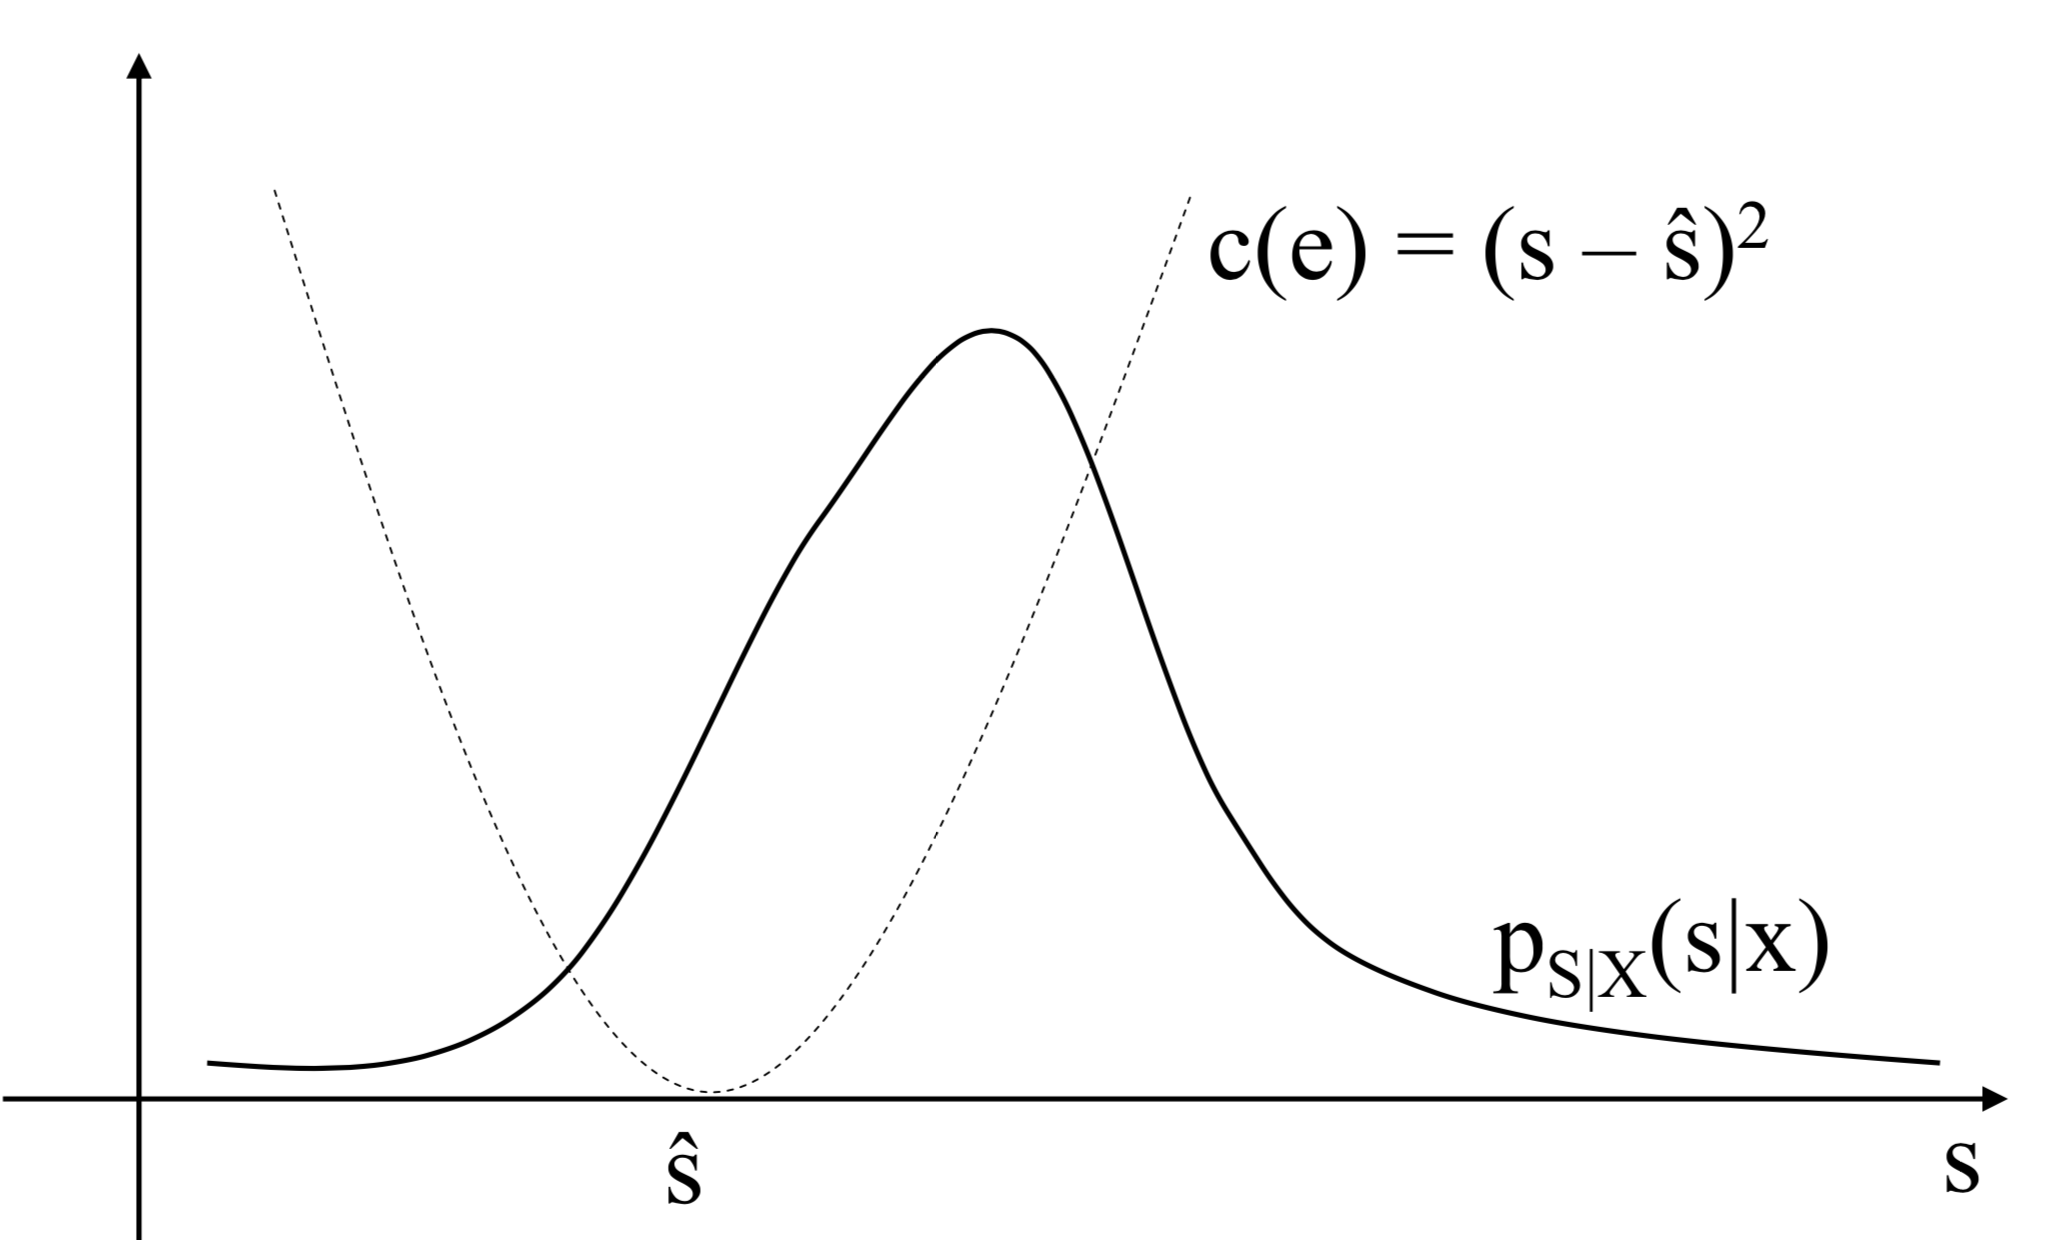
\includegraphics[width=10cm]{Figures//estimador_cuadratico.png}
    \caption{Graphical representation of the process of calculating the posterior mean for a generic value $\hat{s}$.}
    \label{fig:estimador_cuadratico}
  \end{center}
\end{figure}
%%%%%%%%%%%%

The value of $\hat s_{\text{MSE}}$ can be analytically obtained by taking the derivative of the posterior mean cost and equaling the result to 0. The calculation of the derivative does not pose any difficulty since the derivative and the integral can be commutated (it is integrated with respect to $s$ and is derived with respect to $\hat s$):
\begin{equation}
\label{ec:estimador_MSE}
\left.\frac{d \mathbb{E}\{(S-\hat s)^2| {\bf X}={\bf x}\}}{d \hat s}\right|_{\hat s = \hat s_{\text{MSE}}} = -2 \int_s (s - \hat s_{\text{MSE}}) p_{S|{\bf X}}(s|{\bf x}) ds = 0
\end{equation}


Bearing in mind that the integral in \eqref{ec:estimador_MSE} should be cancelled, and using the fact that $\int p_{S|{\bf X}}(s|{\bf x}) ds = 1$, it is easy to demonstrate that the minimum mean squared error estimator of $S$ is given by

\begin{framed}
\begin{equation}
\label{ec:estimador_MSE_final}
\hat s_{\text{MSE}} = \int s\;p_{S|{\bf X}}(s|x) ds = \mathbb{E}\{S|{\bf X} ={\bf x}\}
\end{equation}
\end{framed}

In other words, the minimum mean squared error estimator of $S$ is the mean of $S$ given $\bf X$ or the posterior mean of $S$ , i.e., the expected value of $p_{S|{\bf X}}(s|{\bf x})$.

%%%%%%%%%%%%%%%%
%\begin{exercise}
%Check that the expression \eqref{ec:estimador_MSE_final} actually constitutes a minimum of the given average cost {\bf X}, by calculating the second derivative of $\mathbb{E}\c(S,\hat s)|{bf X} = {\bf x}$.
%\end{exercise}
%%%%%%%%%%%%%%


%%%%%%%%%%%%%%%
\begin{example}[Straightforward calculation of the MSE estimator]
According to \eqref{ec:estimador_MSE_final}, minimum mean squared error estimator obtained in \ref{CalculoECM} can alternatively be obtained as follows

\begin{align}
\label{ec:estimador_MSE_final2}
\hat s_{\text{MSE}} = \int_0^1 s p_{S|X}(s|x) ds   
   = \int_0^x \frac{s}{x} ds 
   = \frac{1}{2} x
\end{align}
which coincides with \eqref{eq:sopt_halfx}.
\end{example}\vspace{0.4cm}
%%%%%%%%%%%%%



%%%%%%%%%%%%%%%%%%%%%%%%%%%%%%%%%%%%%%%%%%%%%%%%%%%%%
\subsection{Minimum Mean Absolute Deviation Estimator (MAD)}

In the same way as we have proceeded in the case of the estimator $\hat s_\text{MSE}$, we can calculate the estimator associated with the absolute deviation of the estimation error, $c(e) = |e| = |s - \hat s|$. This estimator, which we will refer to as the Mean Absolute Deviation (MAD), is characterized by

\begin{equation}
\label{ec:coste_MAD}
\begin{split}
\hat s_{\text{MAD}} & = \arg\min_{\hat s}\; \mathbb{E}\{|S - \hat s|~|{\bf X} = {\bf x} \} = \\
& = \arg\min_{\hat s} \int_s |s - \hat s|\;p_{S|{\bf X}}(s|{\bf x}) ds
\end{split}
\end{equation}


Again, it is simple to illustrate the process of calculating the posterior mean cost by overlapping on the same axes the cost expressed as a function of $s$ and the posterior distribution of the variable to be estimated (see Fig. \ref{fig:estimador_absoluto}). This representation also suggests the convenience of splitting the integral into two parts corresponding to the two slopes of the cost function:


\begin{equation}
\begin{split}
\mathbb{E}\{|S - \hat s|~|{\bf X} = {\bf x} \} &= \int_{-\infty}^{\hat s} (\hat s - s) \;p_{S|{\bf X}}(s|{\bf x}) ds + \int_{\hat s}^\infty (s - \hat s) \;p_{S|{\bf X}}(s|{\bf x}) ds \\
& = \hat s \left[ \int_{-\infty}^{\hat s} p_{S|{\bf X}}(s|{\bf x}) ds -  \int_{\hat s}^{\infty} p_{S|{\bf X}}(s|{\bf x}) ds\right] + \\
&\;\;\;\;\;\;\;\;\;\;\;\; + \int_{\hat s}^{\infty} s\;p_{S|{\bf X}}(s|{\bf x}) ds -  \int_{-\infty}^{\hat s} s \; p_{S|{\bf X}}(s|{\bf x}) ds
\end{split}
\end{equation}

%%%%%%%%%%%%%%
\begin{figure}[t]
  \begin{center}
  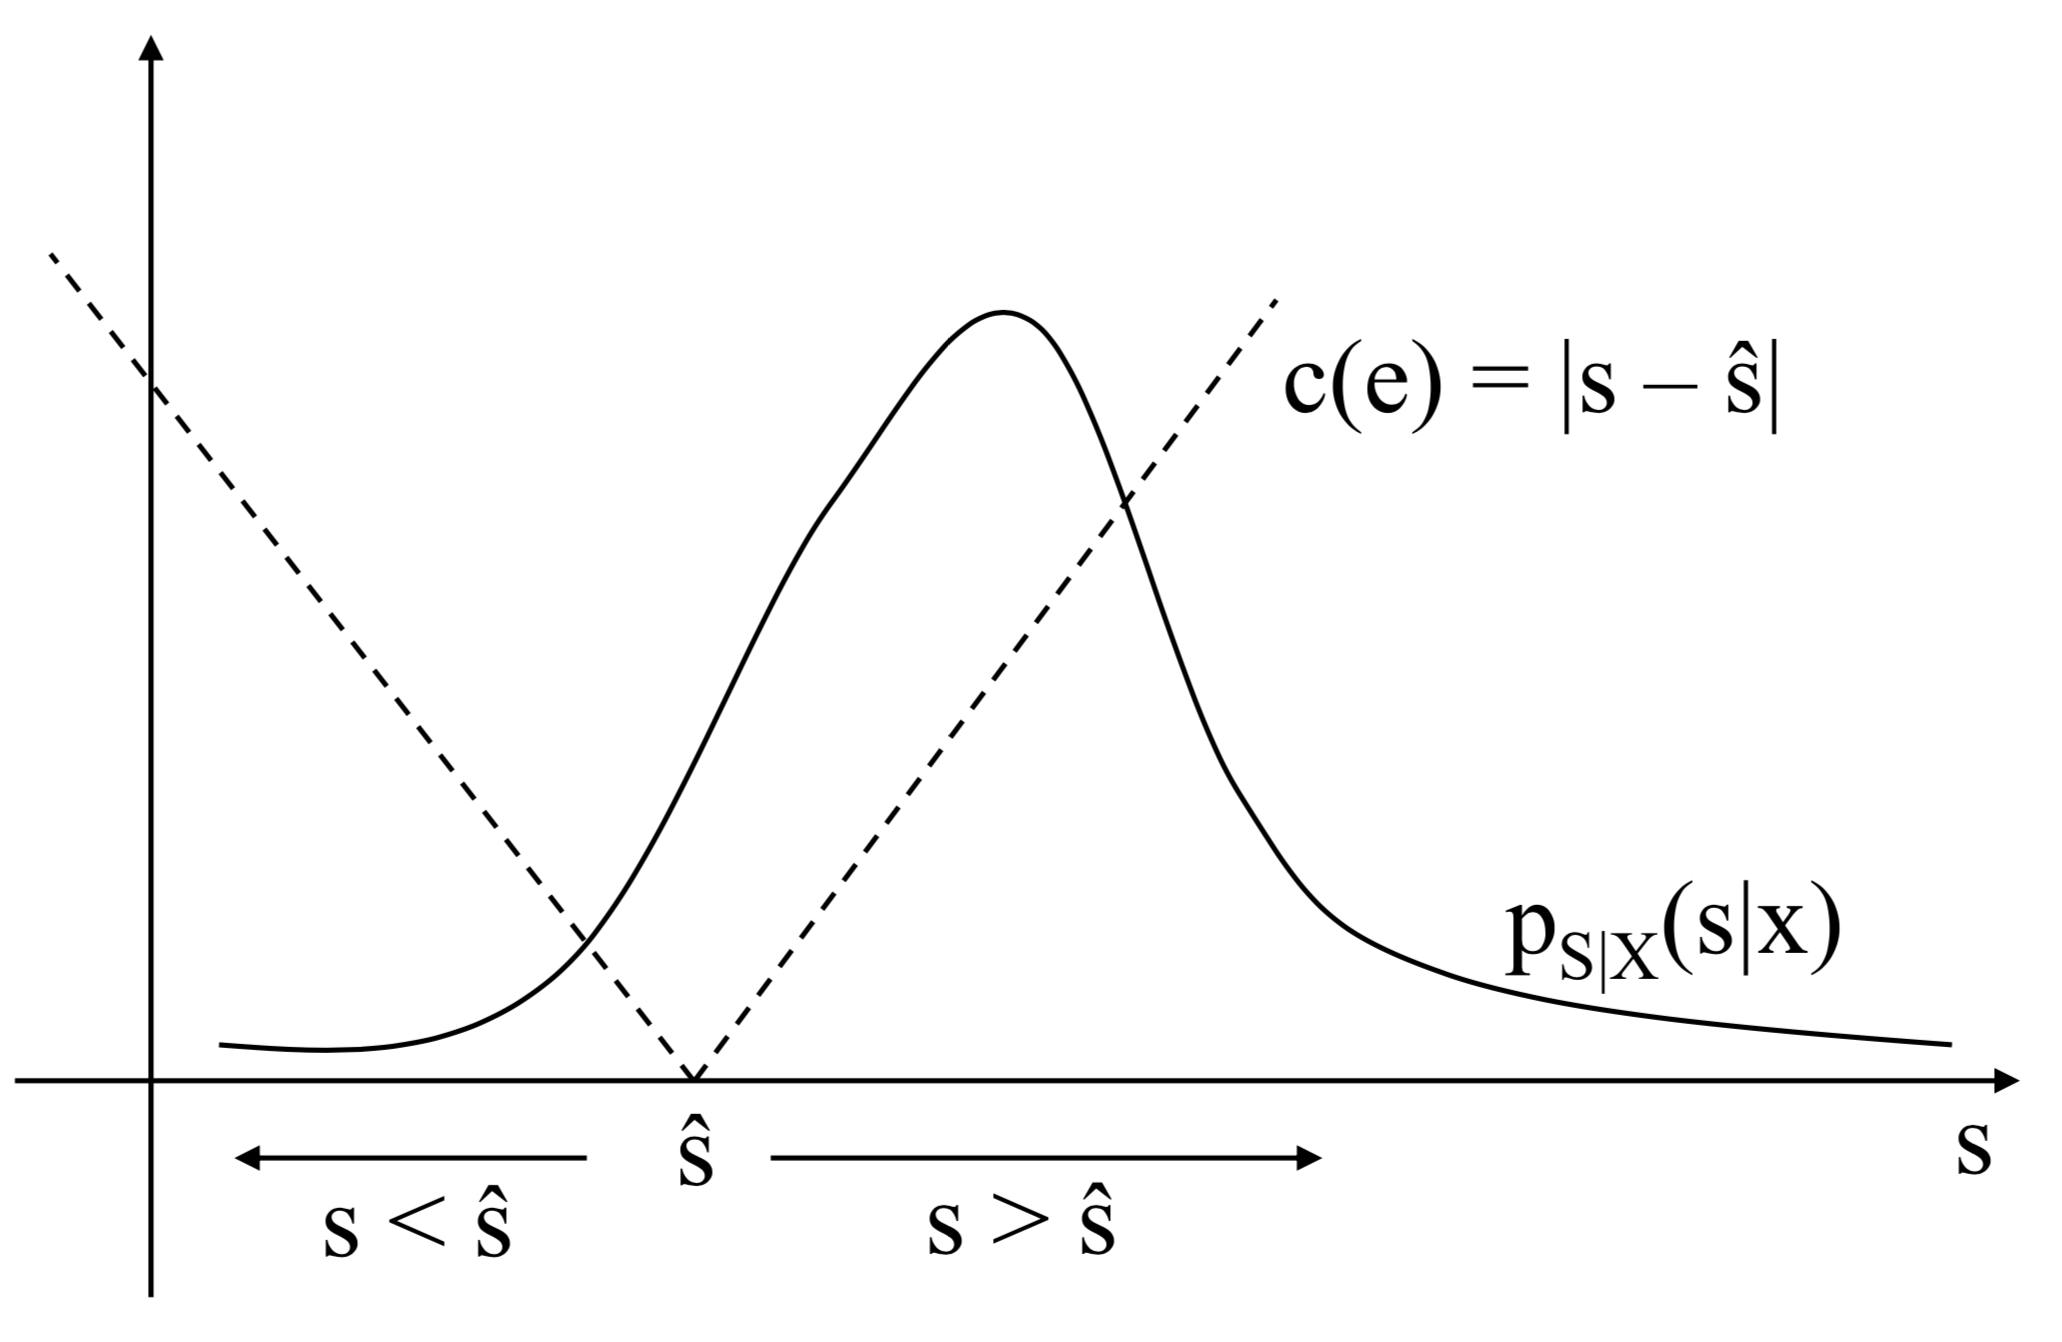
\includegraphics[width=10cm]{Figures//estimador_absoluto.png}
    \caption{Graphical representation of  the process of calculating the posterior mean absolute error for a generic value $\hat s$.}
    \label{fig:estimador_absoluto}
  \end{center}
\end{figure}
%%%%%%%%%%%%

The fundamental theorem of calculus\footnote{$\frac{d}{d x} \int_{t_0}^x g(t) dt = g(x)$.} allows us to obtain the derivative of the posterior mean cost as
\begin{equation}
\frac{d \mathbb{E}\{|S - \hat s|~|{\bf X} = {\bf x} \}}{d \hat s} = 2 F_{S|{\bf X}}(\hat s|{\bf x}) - 1
\end{equation}

where $F_{S|{\bf X}}(s|{\bf x})$ is the posterior distribution function of $S$ given ${\bf X}$. Since $\hat s_{\text{MAD}}$ represents the minimum of the mean cost, the previous derivative must be cancelled for the estimator, verifying that $F_{S|{\bf X}}(\hat s_{\text{MAD}}|{\bf x}) = 1/2$. In other words, the absolute minimum error estimator is given by the median of $p_{S|{\bf X}}(s|{\bf x})$:

\begin{framed}
\begin{equation}
\label{ec:estimador_MAD_final}
\hat s_{\text{MAD}} = \text{median}\{S|{\bf X} ={\bf x}\}
\end{equation}
\end{framed}

Remember that the median of a distribution is the point that separates that distribution into two regions that have the same probability, so the minimum mean absolute error estimator will verify that
{$$P\{S > \hat s_{\text{MAD}}\} = P\{S < \hat s_{\text{MAD}}\}$$}

{\begin{example}[Design of a Minimum Mean Absolute Deviation Estimator]

In the scenario of the example \ref{CalculoECM}, the a posterior distribution of $S$ given $X$ is uniform between 0 and $x$, the median of which is $x/2$. So,

\begin{align}
\label{ec:estimador_MSE_finalej}
\hat s_{\text{MAD}} = \frac{1}{2} x 
\end{align}

Note that, in this case, the MAD estimator matches the MSE obtained at \eqref{eq:sopt_halfx}. This is a consequence of the symmetry of the a posterior distribution. In general, both estimators do not have to coincide.

\end{example}\vspace{0.4cm}
}




%%%%%%%%%%%%%%%%%%%%%%%%%%%%%%%%%%%%%%
\section{Estimation with constrains}
%%%%%%%%%%%%%%%%%%%%%%%%%%%%%%%%%%%%%%


%%%%%%%%%%%%%%%%%%%%%%%%%%%%%%%%%
\subsection{General principles}

Sometimes it may be useful to impose a certain parametric shape on the estimator, $\hat S = f_{\bf w}(\bf X)$, where ${\bf w}$ is a vector containing all the parameters of the function. For example, in a case with two observations ${\bf X} = [X_1, X_2]^T$, it might be a design requirement to restrict the estimator search to the family of quadratic estimators of the form $\hat S = w_0 + w_1 X_1^2 + w_2 X_2^2$. In these cases, the estimator design task is to find the optimal parameter vector ${\bf w}^*$ which provides a minimum average cost subject to the constraint imposed in the estimator architecture:

\begin{align}
{\bf w}^* & = \arg\min_{\bf w}\; \mathbb{E}\{c(S,\hat S)\} = \arg\min_{\bf w} \; \mathbb{E}\{c(S,f_{\bf w}({\bf X}))\} \nonumber\\
 &= \arg\min_{\bf w} \int_{\bf x} \int_s c(s,f_{\bf w}({\bf x})) p_{S,{\bf X}}(s,{\bf x}) ds d{\bf x}
\end{align}

It can easily be understood that the imposition of constraints on the analytical form of the estimator results in incurring a higher average cost than would be obtained using the Bayesian estimator associated with the same cost function\footnote{The only exception to this rule is precisely the case where the constraints imposed allow the optimal estimator to be obtained or, in other words, when the Bayesian estimator presents an analytical form compatible with the constraints imposed.}. However, there may be practical reasons that make the use of the former preferable, for example for simplicity in the design or application of the estimator. An example of this can be found in the Section \ref{sec:est_lineal}, dedicated to the study of linear estimators with minimum mean squared error.

%%%%%%%%%%%%%%%
\begin{example}[{Calculating an Estimator with Constrains}]
\label{CalculoECM_rest}
Continuing the example \ref{CalculoECM2}, we want to calculate the minimum quadratic mean error estimator that has the form $\hat{s} = wx^2$. Starting from the mean cost given the observation calculated in \eqref{Est:ECMsx}, the expression of the global average cost can be obtained as

\begin{equation}
\label{ec:coste_medio2}
\begin{split}
\mathbb{E}\{c(S,\hat S)\} 
   &= \int_{\bf x} \mathbb{E}\{c(S,\hat s)|X=x\} \;p_{\bf X}(\bf x) d{\bf x}  \\
   &= \int_{\bf x} \left(\frac{1}{3}x^2 -\hat{s}x +\hat{s}^2 \right) 
                   p_{\bf X}(\bf x) d{\bf x}
\end{split}
\end{equation}
Forcing $\hat{s} = wx^2$ and taking into account that $p_{\bf X}({\bf x})=1$ for $ 0<x<1$ , you get the global average cost as a function of $w$.
\begin{align}
\mathbb{E}\{c(S,w{\bf X}^2)\} 
   & = \int_{\bf x} \left(\frac{1}{3}x^2 - wx^3 + w^2x^4 \right) d{\bf x} \\
   & = \frac{1}{9} - \frac{1}{4} w + \frac{1}{5} w^2
\label{Est:ECMwx2}
\end{align}
The $w^*$ value that optimizes \eqref{Est:ECMwx2} can be calculated by deriving respect to $w$ and zeroing the expression obtained:
\begin{align}
\left. \frac{d}{d\hat{w}} \mathbb{E}\{c(S,w{\bf X}^2)\} \right|_{w=w^*} 
    &= - \frac{1}{4} + \frac{2}{5} w^* =0,
\end{align}
\begin{equation}
\label{eq:sopt_58}
w^* = \frac{5}{8},
\end{equation}
and therefore the estimator sought is: $\hat{s} = \frac{5}{8}x^2$.

\end{example}\vspace{0.4cm}
%%%%%%%%%%%%%


%%%%%%%%%%%%%%%%%%%%%%%%%%%%%%%%%%%%%%%%%%%%%%%%%%%%%%%%%%%%%%%
\subsection{Linear estimation of minimum squared mean error}
\label{sec:est_lineal}

In this section we will focus on the study of random variable estimators that obtain their output as a linear combination of the values of the observations, using the minimization of the mean squared error as design criterion. Therefore, we will exclusively consider estimators that calculate their output as
\begin{equation}
\hat S = w_0 + w_1 X_1 + \dots + w_N X_N
\end{equation}

where $N$ denotes the number of available observable variables, $\{X_i\}_{i=1}^N$, and $\{w_i\}_{i=0}^{N}$ are the weights that characterize the estimator. In this context, it is common to refer to the term independent of the above expression, $w_0$, as a bias term. For analytical simplicity, it is more convenient to enter the following matrix notation:

\begin{equation}
\hat S = w_0 + {\bf w}^T {\bf X} = {\bf w}_{\text{e}}^T {\bf X}_{\text{e}}
\label{Est:Sestlineal}
\end{equation}
where ${\bf w} = [w_1,\dots,w_N]^T$ and ${\bf X} = [X_1,\dots,X_N]^T$ are the (column) vectors  of parameters and observations, respectively, and ${\bf w}_{\text{e}} = [w_0, {\bf w}^T]^T$ and ${\bf X}_{\text{e}} = [1, {\bf X}^T]^T$ are extended versions of these vectors.

It can be understood that, by imposing a restriction on the analytical form implemented by the estimator, linear estimators will generally obtain lower performance than the optimal Bayesian estimator. However, the interest of linear estimators is justified by their simplicity and ease of design. As we shall see, for the calculation of the linear estimator of minimum squared mean error, it will be sufficient to know the first and second order statistical moments (means and covariances) associated with the observable variables and the variable to be estimated.

%On the other hand, the use of linear estimators is fully justified in certain circumstances, for example when dealing with variables with Gaussian distributions, since, as we saw in the previous section, in this case the Bayesian estimator with the minimum squared mean error has a linear architecture. 


%%%%%%%%%%%%%%%%%%%%%%%%%%%%%%%%%%%%%%%%%%%%%%%%%%%%%%%%%%%%%%%%%%%%%%
\subsubsection{Minimization of the {mean squared error}.}% y ecuaciones normales}

As we have already mentioned, we will consider as design criteria the squared error, $c(e) = (s-\hat s)^2$, so the optimal weight vector will be the one that minimizes the average value of this cost function:

\begin{equation}
{\bf w}_\text{e}^* = \arg\min_{{\bf w}_\text{e}} \; \mathbb{E}\{(S - \hat S)^2\} =  \arg\min_{{\bf w}_\text{e}}\;  \mathbb{E}\{(S - {\bf w}_{\text{e}}^T {\bf X}_{\text{e}})^2\}
\end{equation}
and we will refer to the linear estimator associated with this optimal weight vector as $\hat S_\text{LMSE}$: 
$$\hat S_\text{LMSE} = {{\bf w}_{\text{e}}^*}^T {\bf X}_{\text{e}}$$

%%%%%%%%%%%%%%
\begin{figure}[htb]
  \begin{center}
  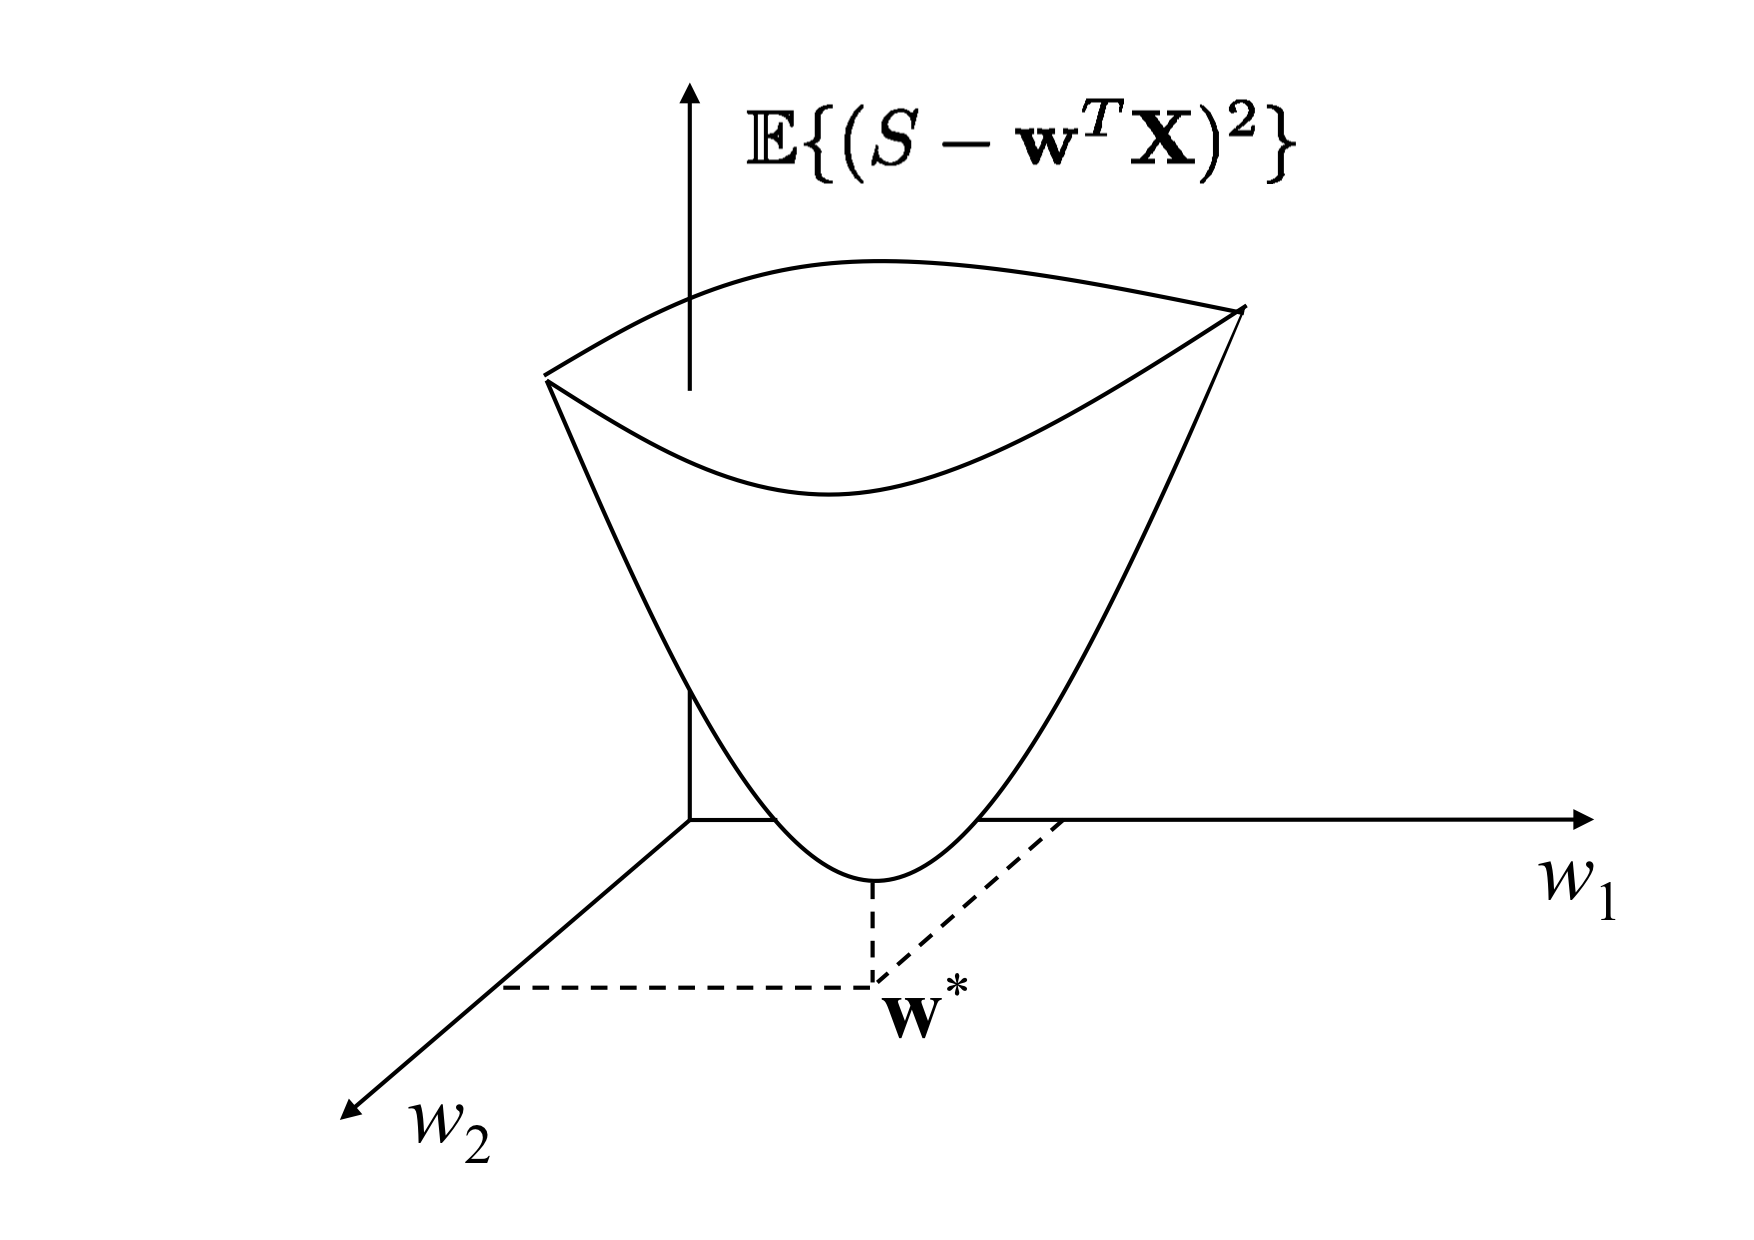
\includegraphics[width=10cm]{Figures//linear_est_error_surface.png}
    \caption{Surface of the mean squared error of the linear estimator as a function of the estimator weights.}
    \label{fig:linear_est_error_surface}
  \end{center}
\end{figure}
%%%%%%%%%%%%

Figure \ref{fig:linear_est_error_surface} represents the error surface in a case with two observations. Being the function to minimize quadratic in weights (minimization argument), the error surface will take the form of a $N$ dimensional paraboloid. In addition, since the average cost is not negative, it is guaranteed that the function is convex, and its minimum can be located by equaling $\bf 0$ the gradient of the average cost with respect to the weight vector\footnote{The gradient of a function scale $f({\bf w})$ with respect to the vector ${\bf w}$ is defined as a vector formed by the derivatives of the function with respect to each one of the components of $\bf w$: $\nabla_{{\bf w}} f({\bf w}) = \left[\frac{\partial f}{\partial w_1}, \dots \frac{\partial f}{\partial w_N}\right]^T$.}:

\begin{equation}
\label{ec:ecs_normales_1}
\begin{split}
\left. \nabla_{{\bf w}_{\text{e}}} \mathbb{E}\{(S - \hat S)^2\} \right|_{{\bf w}_{\text{e}} 
   = {\bf w}_{\text{e}}^*} 
 & = \left. -2 \mathbb{E}\{(S - {\bf w}_{\text{e}}^T {\bf X}_{\text{e}}) {\bf X}_{\text{e}} \} \right|_{{\bf w}_{\text{e}} = {\bf w}_{\text{e}}^*} = \\
 & = -2 \mathbb{E}\{(S -  {{\bf w}_{\text{e}}^*}^T {\bf X}_{\text{e}}) {\bf X}_{\text{e}} \} = {\bf 0}
\end{split}
\end{equation}

The second line of the above expression defines the conditions to be met by the optimal weight vector. Note that this equation is actually a system of $N+1$ equations (as many as dimensions have ${\bf X}_{\text{e}}$) with $N+1$ unknowns (the components of ${\bf w}_{\text{e}^*}$).

In order to find the optimal {weight} vector, it is convenient to rewrite the last line of \eqref{ec:ecs_normales_1} as follows 

\begin{equation}
\mathbb{E}\{S {\bf X}_{\text{e}} \}
    = \mathbb{E}\{ {\bf X}_\text{e} ({\bf X}_{\text{e}}^T {\bf w}_{\text{e}}^*)  \}
\label{Est:EcDelELv}
\end{equation}
Defining the cross-correlation vector
\begin{equation}
{\bf r}_{S{\bf X}_e} = \mathbb{E}\{S{\bf X}_e\}
\end{equation}
and the correlation matrix 
\begin{equation}
{{\bf R}_{{\bf X}_e}} = \mathbb{E}\{{\bf X}_e{\bf X}_e^T\}
\end{equation}
(which is a symmetrical matrix) ec. \eqref{Est:EcDelELv} can be written as
\begin{equation}
\label{Est.ec:RxWr}
{\bf r}_{S{\bf X}_e} = {{\bf R}_{{\bf X}_e}} {\bf w}_{\text{e}}^* 
\end{equation}
Thus, the searched weight vector is:
\begin{framed}
\begin{equation}
\label{Est.ec:weopt}
 {\bf w}_{\text{e}}^* = {{\bf R}_{{\bf X}_e}^{-1}} {\bf r}_{S{\bf X}_e} 
\end{equation}
\end{framed}



%%%%%%%%%%%%%%%%%%%%%%%%%%%%%%%%%%%%%%%%%%%%%%%%%%%%%%%
\subsubsection{Properties of the optimal linear estimator}

Equation \eqref{Est.ec:RxWr} solves the problem of calculating the weights of the estimator $\hat S_\text{LMSE}$. But it is interesting to return to the vector equation  \eqref{ec:ecs_normales_1} to analyze some of its properties. Note that the term in parentheses in this equation is the estimation error
\begin{equation}
E^* = S - {{\bf w}_{\text{e}}^*}^T {\bf X}_{\text{e}}
\end{equation}
so we can rewrite \eqref{ec:ecs_normales_1} as
\begin{equation}
\label{Est:SLMSinsesgado0}
\mathbb{E}\{E^* {\bf X}_{\text{e}})\} = {\bf 0}
\end{equation}
Taking, on the one hand, the first component of this equation (taking into account that $X_{\text{e},1}=1$, and the rest on the other hand, two fundamental properties of the lowest quadratic mean error linear estimator are obtained:
\begin{description}
\item[{\bf Property 1:}] The error has zero mean:
\begin{equation}
\label{Est:SLMSinsesgado}
\mathbb{E}\{E^*\} = {\bf 0}
\end{equation}
When an estimator has this property it is said that it is {\bf unbiased}.% {Volveremos sobre esta propiedad en la sec. \ref{Est:Sec:CaracterEstim}.}
\item [{\bf Property 2 (Orthogonality Principle):}] the error is statistically orthogonal to the observations:
\begin{equation}
\label{Est:PrincipioOrtV1}
\mathbb{E}\{E^* {\bf X}\} = {\bf 0}
\end{equation}
\end{description}



%%%%%%%%%%%%%%%%%%%%%%%%%%%%%%%%%%%%%%%%%%%%%%%%%%%%%%%%%%%%%%%%%%
\subsubsection{{Alternative expression of the estimator}}
Expanding Ecs. \eqref{Est:SLMSinsesgado} and \eqref{Est:PrincipioOrtV1}, we can obtain the following explicit formulas for the coefficients $w_0^*$ and ${\bf w}^*$ of the estimator:

\begin{framed}
\begin{equation}
w_0^* = m_S - {{\bf w}^*}^T{\bf m_x} 
\label{ec:solucionw0}
\end{equation}
\begin{equation}
\label{ec:solucionw}
{\bf w}^* = {{\bf V}_{\bf X}^{-1}} \; {\bf v}_{S,{\bf X}}\end{equation}
\end{framed}

It can be observed that the role of the bias term $w_0$ is to compensate for differences between the means of the variable to be estimated and the observations. Therefore, when all the variables involved have null means, $w_0^* = 0$. In contrast to the paper of $w_0$, we can affirm that the weight vector ${\bf w}$ minimizes the mean quadratic error of the fluctuations of $S$ around its mean, exploiting for it the existing statistical relation between $S$ and $\bf X$.

We will dedicate this section to obtaining the expressions \eqref{ec:solucionw0} and \eqref{ec:solucionw}. The first is a direct consequence of \eqref{Est:SLMSinsesgado} that can be developed as 

\begin{equation}
m_S - {{\bf w}^*}^T{\bf m_x} - w_0^* =0 
\end{equation}
solving for $w_0^*$, we obtain \eqref{ec:solucionw0}.

{We will now search for an expression for ${\bf w}^*$. From \eqref{Est:PrincipioOrtV1} results
\begin{equation}
\label{Est:PrincipioOrtV2}
\mathbb{E}\{(S - {{{\bf w}^*}^T} {\bf X} - w_0^*) {\bf X}\} = {\bf 0}
\end{equation}
which can be rewritten as
\begin{align}
\label{Est:PrincipioOrtV2b}
\mathbb{E}\{S {\bf X}\} 
   &= \mathbb{E}\{({{\bf w}^*}^T {\bf X} + {w_0^*}) {\bf X}\}     \nonumber\\
   &= \mathbb{E}\{{\bf X} ({{\bf X}^T{\bf w}^*}) \} {+ w_0^*} \mathbb{E}\{{\bf X} \}  \nonumber\\
   &= \mathbb{E}\{{\bf X} {\bf X}^T \}{\bf w}^* + w_0^* {\bf m_X}  
\end{align}
}
Now using the expressions that relate the correlation and covariance of two variables:
\begin{equation}
\mathbb{E}\{S {\bf X}\} = {\bf v}_{S,{\bf X}} + m_S {\bf m_X}
\end{equation}
\begin{equation}
\mathbb{E}\{{\bf X}{\bf X}^T\} = {\bf V_X} + {\bf m_X}{\bf m}_{\bf X}^T
\end{equation}
eq. \eqref{Est:PrincipioOrtV2b} becomes 
\begin{align}
\label{Est:PrincipioOrtV3}
{\bf v}_{S,{\bf X}}  
   &= {\bf V_X}{\bf w}^* + {\bf m_X}{\bf m}_{\bf X}^T{\bf w}^* + w_0^* {\bf m_X} - m_S {\bf m_X}  \nonumber\\ 
   &= {\bf V_X}{\bf w}^* 
    + {\bf m_X}(w_0^* + {\bf m}_{\bf X}^T{\bf w}^* - m_S) 
     \nonumber\\ 
   &= {\bf V_X}{\bf w}^* 
\end{align}
where, in the last equality, we have applied \eqref{ec:solucionw0}. So, solving for ${\bf w}^*$, we get \eqref{ec:solucionw}.



%%%%%%%%%%%%%%%%%%%%%%%%%%%%%%%%%%%%%%%%%%%%%%%%%%%%%%%%%%%%
\subsubsection{Minimum squared mean error}

Here we will calculate the mean squared error associated with the linear estimator of minimum mean squared error, $\hat S_\text{LMSE}$. As commented at the beginning of this section, the mean squared  error obtained will, in general, be higher than the minimum mean squared error of the Bayesian estimator ($\hat S_\text{MMSE}$), except when this last estimator has precisely a linear structure (in this case, it would be the same).

To calculate the mean squared error we only have to develop the expression of the mean quadratic error, particularizing it for $\hat S_\text{LMSE}$ and leaving the result in function of the mathematical expectations of the involved random variables:

\begin{align}
\mathbb{E}\{(S - \hat S_\text{LMSE})^2\} 
   & = \mathbb{E}\{E^*(S - w_0^* - {{\bf w}^*}^T {\bf X})\} \nonumber\\ 
   & = \mathbb{E}\{E^* S\} 
     - w_0^* \mathbb{E}\{E^*\} 
     - {{\bf w}^*}^T \mathbb{E}\{{\bf X}E^*\}  \nonumber\\
   & = \mathbb{E}\{E^* S\} 
\end{align}

where, in the last equality, we have applied the two properties of the minimum quadratic mean error estimator obtained in \eqref{Est:SLMSinsesgado} and \eqref{Est:PrincipioOrtV1}. Operating again the error term, $E^*$, results in
\begin{align}
\mathbb{E}\{(S - \hat S_\text{LMSE})^2\} 
   & = \mathbb{E}\{S (S - w_0^* - {{\bf w}^*}^T {\bf X})\}  \nonumber\\
   & = \mathbb{E}\{S^2\} 
     - w_0^* m_S 
     - {{\bf w}^*}^T ({\bf v}_{S{\bf X}} + m_S {\bf m}_{\bf X})\} \nonumber\\
   & = \mathbb{E}\{S^2\} - m_S (w_0^* {+} {{\bf w}^*}^T {\bf m}_{\bf X})
     - {{\bf w}^*}^T {\bf v}_{S{\bf X}}  \nonumber\\
   & = v_S - {{\bf w}^*}^T {\bf v}_{S{\bf X}} 
\end{align}
%\begin{equation}
%\begin{split}
%\mathbb{E}\{(S - \hat S_\text{LMSE})^2\} 
%   & = \mathbb{E}\{(S - w_0^* - {{\bf w}^*}^T {\bf X})^2\} \\ 
%   & = \mathbb{E}\{S^2\} + {w_0^*}^2 + {{\bf w}^*}^T \mathbb{E}\{{\bf X}{\bf X}^T\}{{\bf w}^*} - 2 w_0^* \mathbb{E}\{S\} \\ 
%& \;\;\;\;\;\; - 2 {{\bf w}^*}^T \mathbb{E}\{S {\bf X}\} - 2 w_0^* {{\bf w}^*}^T \mathbb{E}\{{\bf X}\}
%\end{split}
%\end{equation}
%
%Si introducimos en esta expresión los valores de los pesos óptimos [Ecs. \eqref{ec:solucionw} y \eqref{ec:solucionw0}], y tenemos también en cuenta que $\mathbb{E}\{S^2\} = v_S + \mathbb{E}^2\{S\}$, así como las expresiones análogas para $\mathbb{E}\{S {\bf X}\}$ y $\mathbb{E}\{{\bf X}{\bf X}^T\}$, se puede demostrar que
%\begin{equation}\label{ec:err_LMSE}
%\mathbb{E}\{(S - \hat S_\text{LMSE})^2\} 
%    = v_S - {\bf v}_{S,{\bf X}}^T \; {{\bf V}_{\bf X}^{-1}} \; {\bf v}_{S,{\bf X}}
%\end{equation}
%\end{example}\vspace{0.4cm}

%\begin{exercise}[Cálculo del error cuadrático medio para variables con medias nulas]
%Demuestre el resultado \eqref{ec:err_LMSE} para el caso concreto en que $\mathbb{E}\{S\} = 0$ y $\mathbb{E}\{{\bf X}\} = {\bf 0}.$
%\end{exercise}

%%%%%%%%%%%%%%%%
\begin{exercise}[Linear estimation of minimum mean squared error]
We want to construct a linear estimator of minimum mean squared error that will allow us to estimate the random variable $S$ from the random variables $X_1$ and $X_2$. Knowing that
\begin{equation}
\begin{array}{lll} \mathbb{E}\{S\} = 1/2 & \mathbb{E}\{X_1\} = 1 & \mathbb{E}\{X_2\} = 0 \\ \mathbb{E}\{S^2\} = 4 & \mathbb{E}\{X_1^2\} = 3/2 & \mathbb{E}\{X_2^2\} = 2 \\ \mathbb{E}\{S X_1\} = 1 \;\;\;\;& \mathbb{E}\{S X_2\} = 2 \;\;\;\; & \mathbb{E}\{X_1 X_2\} = 1/2 \end{array}\nonumber
\end{equation}
get the weights from the desired estimator and calculate its squared mean error. Calculate the estimated value for the observation vector: $[X_1,X_2] = [3, 1]$.
\end{exercise}
%%%%%%%%%%%%%%
%%%%%%%%%%%%%%%%%%%%%%%%%%%%%%%%%%%%%%
\section{Estimation with gaussian distributions}
%%%%%%%%%%%%%%%%%%%%%%%%%%%%%%%%%%%%%%

In this section we will analyze the case of random variable estimation when the combined distribution of all the variables involved (variable to be estimated and observation variables) is a multidimensional Gaussian. This case is of special interest given the frequency with which these distributions usually appear in problems in the field of telecommunications and in other scenarios. In this case, it can be shown that all marginal distributions and all conditional distributions are also Gaussian. Specifically, given that $p_{S|{\bf X}} (s|{\bf x})$ is Gaussian, it can be understood that the fashion, the mean and the median of the distribution coincide, so $\hat{s}_{\text{MSE}} = \hat{s}_{\text{MAD}} = \hat{s}_{\text{MAP}}$ will be verified. Therefore, during this section we will focus our discussion on the calculation of the minimum quadratic mean error estimator. 

Besides, we will demonstrate that the MSE estimator and, consequently, the MAP and MAD estimators are linear, which will allow us to use the results shown in the previous section for minimum mean squared error estimators.


%%%%%%%%%%%%%%%%%%%%%%%%%%%%%%%%
\subsection{One dimensional case}

We will consider as a starting point a case with one-dimensional random variables with zero means, in which the joint distribution of $X$ and $S$ has the following form:

\begin{equation}
p_{S,X}(s,x) \sim G\left(\left[\begin{array}{c} 0 \\ 0 \end{array}\right],\left[\begin{array}{cc} v_S & \rho \\ \rho & v_X \end{array}\right]\right)
\end{equation}
where $\rho$ is the covariance between the two random variables.

From this joint distribution we can obtain any other distribution involving the variables $s$ and $x$; specifically, the posterior distribution of $S$ can be obtained as:

\begin{equation}
\begin{split}
p_{S|X}(s|x) & = \frac{p_{S,X}(s,x)}{p_X(x)} \\
& = \displaystyle\frac{\displaystyle\frac{1}{2\pi \sqrt{v_X v_S - \rho^2}}\exp\left[-\displaystyle\frac{1}{2(v_X v_S - \rho^2)}\left[\begin{array}{c} s \\ x \end{array}\right]^T\left[\begin{array}{cc} v_X & -\rho \\ -\rho & v_S \end{array}\right] \left[\begin{array}{c} s \\ x \end{array}\right]\right]}{\displaystyle\frac{1}{\sqrt{2\pi v_X}} \exp\left[-\displaystyle\frac{x^2}{2 v_X}\right]}
\end{split}
\end{equation}

where it has been necessary to calculate the inverse of the covariance matrix of $S$ and $X$, which is easy since the matrix has dimensions of $2 \times 2$.

Our goal for obtaining $\hat s_{\text{MSE}}$ is to calculate the mean of that distribution. However, a direct calculation by integrating your product with $s$ is quite complicated. However, given the joint Gaussian character of $S$ and $X$, we know that the posterior distribution of $S$ must necessarily be Gaussian, defined by its (unknown) parameters of mean and variance $m_{S|X}$ and $v_{S|X}$, respectively, allowing the above expression to be rewritten as:

\begin{multline}
\frac{1}{\sqrt{2\pi v_{S|X}}} \exp\left[ -\frac{(s - m_{S|X})^2}{2 v_{S|X}}\right] = \\ \displaystyle\frac{\displaystyle\frac{1}{2\pi \sqrt{v_X v_S - \rho^2}}\exp\left[-\displaystyle\frac{1}{2(v_X v_S - \rho^2)}\left[\begin{array}{c} s \\ x \end{array}\right]^T\left[\begin{array}{cc} v_X & -\rho \\ -\rho & v_S \end{array}\right] \left[\begin{array}{c} s \\ x \end{array}\right]\right]}{\displaystyle\frac{1}{\sqrt{2\pi v_X}} \exp\left[-\displaystyle\frac{x^2}{2 v_X}\right]}
\end{multline}
It is possible to break this equality down into two others associated with factors external to the exponentials and their arguments:

\begin{equation}
\label{ec:gauss_iguald1}
\frac{1}{\sqrt{2\pi v_{S|X}}} = \frac{\sqrt{2\pi v_X}}{{2\pi \sqrt{v_X v_S - \rho^2}}}
\end{equation}
\begin{equation}
\label{ec:gauss_iguald2}
\frac{(s - m_{S|X})^2}{v_{S|X}} = \displaystyle\frac{1}{v_X v_S - \rho^2}\left[\begin{array}{c} s \\ x \end{array}\right]^T\left[\begin{array}{cc} v_X & -\rho \\ -\rho & v_S \end{array}\right] \left[\begin{array}{c} s \\ x \end{array}\right] - \displaystyle\frac{x^2}{v_X}
\end{equation}
By operating the matrix terms, the second of these equals can be more simply rewritten as
\begin{equation}
\label{ec:gauss_iguald2bis}
\frac{(s - m_{S|X})^2}{v_{S|X}} = \displaystyle\frac{v_X s^2 + v_S x^2 - 2 \rho x s}{v_X v_S - \rho^2} - \displaystyle\frac{x^2}{v_X}
\end{equation}

Note that \eqref{ec:gauss_iguald2bis} assumes an equality between two polynomials in $s$ (and in $x$). Therefore, the coefficients of the independent, linear and quadratic terms in $s$ (i.e., which do not depend on $s$, or which multiply to $s$ and $s^2$) that appear on both sides of the equality must match. Therefore, and taking into account that $m_{S|X}$ does not depend on $s$, the following three equality must be verified:

\begin{equation}
\label{ec:gauss_iguald3}
\frac{m_{S|X}^2}{v_{S|X}} = \displaystyle\frac{v_S x^2}{v_X v_S - \rho^2} - \displaystyle\frac{x^2}{v_X}
\end{equation}
\begin{equation}
\label{ec:gauss_iguald4}
\frac{s\;m_{S|X}}{v_{S|X}} = \displaystyle\frac{\rho x s}{v_X v_S - \rho^2}
\end{equation}
\begin{equation}
\label{ec:gauss_iguald5}
\frac{s^2}{v_{S|X}} = \displaystyle\frac{v_X s^2}{v_X v_S - \rho^2}
\end{equation}
For the calculation of the posterior mean, it is convenient solving \eqref{ec:gauss_iguald4} for $m_{S|X}$ as
\begin{equation}
\label{ec:msx_parcial}
m_{S|X} = \frac{v_{S|X} \rho x}{v_X v_S - \rho^2}
\end{equation}
Finally, the value of the posterior variance can easily be extracted from \eqref{ec:gauss_iguald1} or \eqref{ec:gauss_iguald5} as
\begin{equation}
v_{S|X} = \frac{v_X v_S - \rho^2}{v_X}
\end{equation}
Replacing this value in \eqref{ec:msx_parcial} gives the expression that determines the minimum quadratic mean error estimator.
\begin{framed}
\begin{equation}
\label{ec_estimador_caso_gaussiano_final}
\hat s_{\text{MSE}} = m_{S|X} = \frac{\rho}{v_X} x
\end{equation}
\end{framed}
As can be seen, the estimator obtained is \underline{linear}.

%%%%%%%%%%%%%%%%
\begin{exercise}
Generalize the above result for the case where the variables $S$ and $X$ have (non-zero) means $m_S$ and $m_X$, respectively. Demonstrate that in such a case, the estimator is
\begin{equation}
\hat s_{\text{MSE}} = m_S + \frac{\rho}{v_X} (x - m_X)
\end{equation}
\end{exercise}
%%%%%%%%%%%%%%

%%%%%%%%%%%%%%%
\begin{example}[Estimation of a Gaussian signal contaminated by Gaussian noise]
\label{ex:senialenruido}

In this example we will consider the case in which the observation is obtained as the sum of the signal to be estimated and a noise component independent of the signal: $X = S + R$. Both the signal and the noise present Gaussian distributions of zero means and variances $v_S$ and $v_R$, respectively.

Figure \eqref{fig:estimacion_caso_gauss} represents the situation described for a case with $v_S < v_R$.
\begin{figure}[htb]
  \begin{center}
  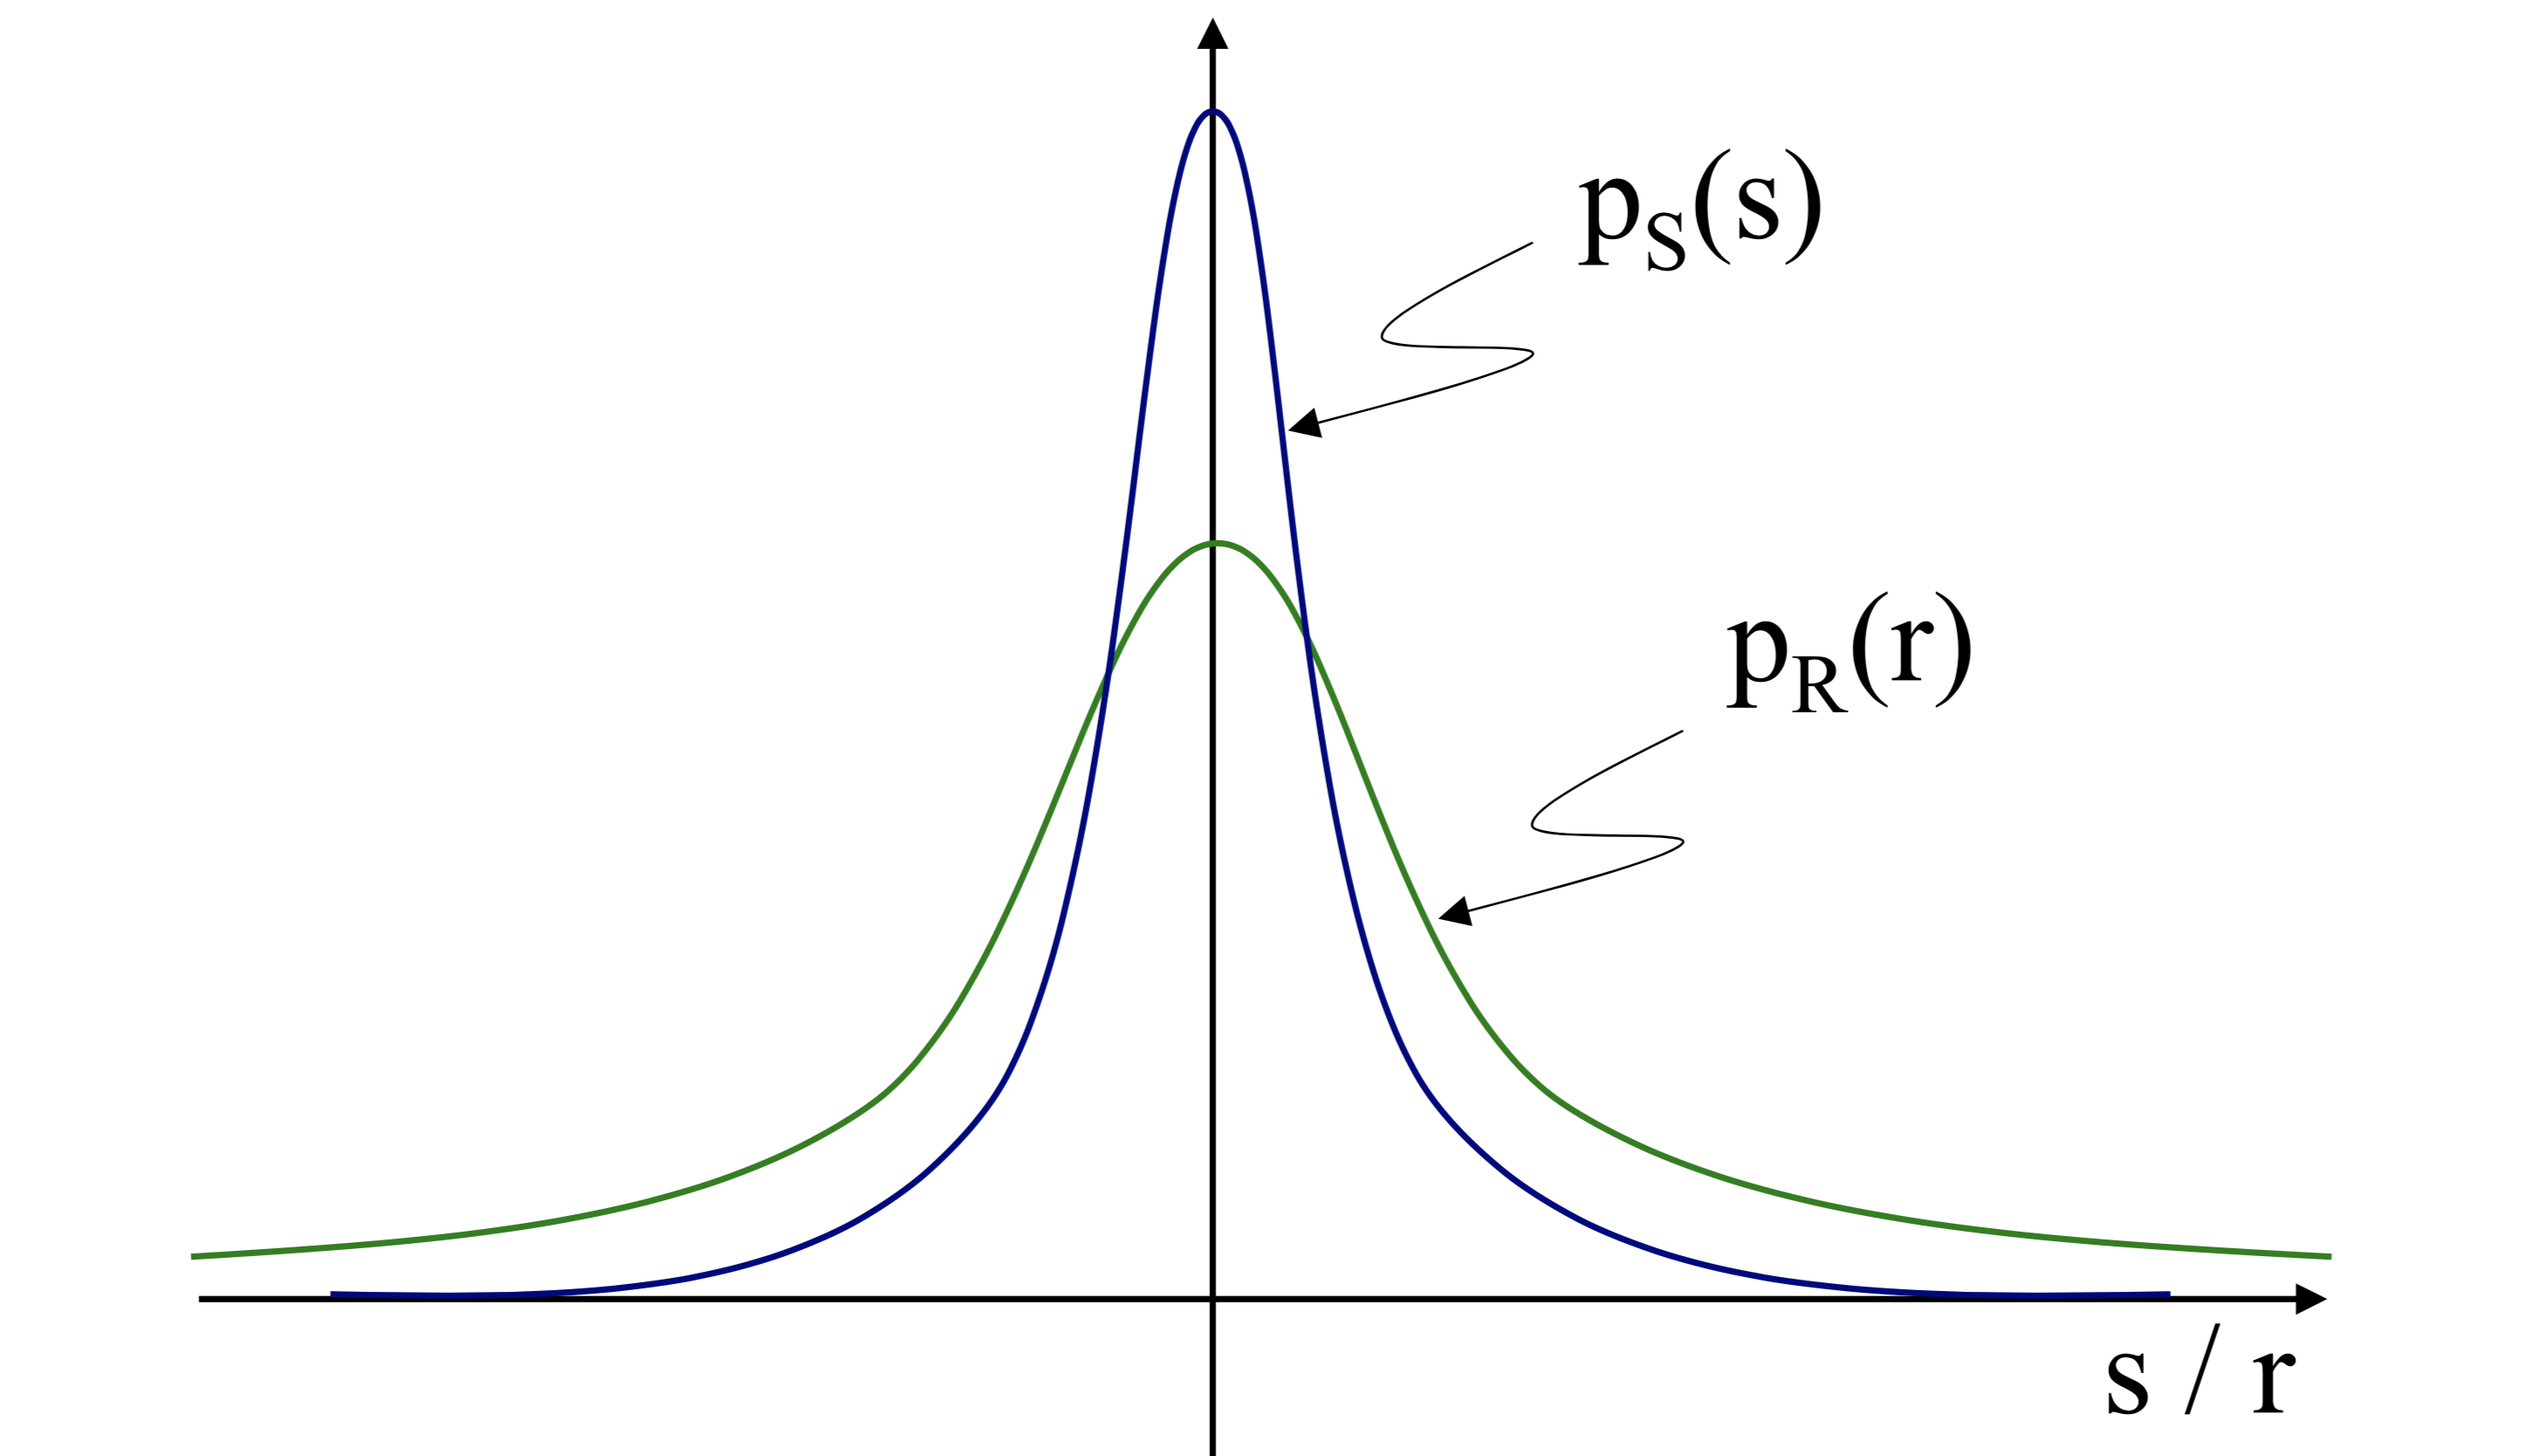
\includegraphics[width=10cm]{Figures//estimacion_caso_gauss.png}
    \caption{Estimation of Gaussian random variable $S$ contaminated by Gaussian noise $R$.}
    \label{fig:estimacion_caso_gauss}
  \end{center}
\end{figure}
\end{example}\vspace{0.4cm}
%%%%%%%%%%%%%

According to \eqref{ec_estimador_caso_gaussiano_final}, for the resolution of the problem we must find the variance of $X$ and the covariance between $S$ and $X$ ($\rho$). The variance $v_X$ is obtained simply as the sum of $v_S$ and $v_R$ because both are independent variables. For the covariance calculation we can proceed as follows:

\begin{equation}
\rho = \mathbb{E} \{(X-m_X)(S-m_S)\} = \mathbb{E} \{X\;S\} = \mathbb{E} \{(S + R) S\} = \mathbb{E} \{S^2\} + \mathbb{E} \{S\;R\} = v_S
\end{equation}

where independence of $S$ and $R$ has been used, and the fact that all variables (including $X$) have zero means.

Replacing these results in \eqref{ec_estimador_caso_gaussiano_final} we get

\begin{equation}
\hat s_{\text{MSE}} = \frac{v_S}{v_S + v_R} x
\end{equation}

This result can be interpreted quite intuitively: when the variance of the noise is much lower than that of the signal (high Signal to Noise Ratio (SNR), $v_S \gg v_R$) you have to  $\hat s_{\text{MSE}} \to x$, which makes sense since the effect of the noise component in this case is not very significant; on the contrary, when the SNR is very low ($v_S \ll v_R$), the observation barely provides information about the $S$ value in each experiment, so the estimator keeps the mean value of the signal component, $\hat s_{\text{MSE}} \to 0$.


%%%%%%%%%%%%%%%%%%%%%%%%%%%%%%%%%%%%%%%%%%%%%%%%%%
\subsection{Case with multidimensional variables}

{In a general multidimensional case, ${\bf S}$ and ${\bf X}$ can be random vectors of dimensions $N$ and $M$, respectively, with joint Gaussian distribution.
\begin{equation}
p_{{\bf S},{\bf X}}({\bf s},{\bf x}) 
   \sim G\left(\left[\begin{array}{c} {\bf m_S} \\ {\bf m_X} \end{array}\right],
               \left[\begin{array}{cc} {\bf V_S}          & {\bf V_{SX}}   \\ 
                                       {\bf V}_{\bf SX}^T & {\bf V_{X}}   
                     \end{array}\right]\right)
\end{equation}
being ${\bf m_S}$ and ${\bf m_X}$ the means of $ {\bf S}$ and $ {\bf X}$, respectively, ${\bf V_S}$ and ${\bf V_X}$ the covariance matrix of ${\bf S}$ and  ${\bf X}$, respectively, and ${\bf V_{SX}}$ the matrix of crossed covariances of ${\bf S}$ and ${\bf X}$, that is,
\begin{equation}
{\bf V_S} = \mathbb{E}\{({\bf S}-{\bf m_S})({\bf S}-{\bf m_S})^T\} \\
\end{equation}
\begin{equation}
{\bf V_X} = \mathbb{E}\{({\bf X}-{\bf m_X})({\bf X}-{\bf m_X})^T\}
\end{equation}
\begin{equation}
{\bf V_{SX}} = \mathbb{E}\{({\bf S}-{\bf m_S})({\bf X}-{\bf m_X})^T\}
\end{equation}
%La expresión general de la densidad de probabilidad es, por tanto
%\begin{align}
%p_{{\bf S},{\bf X}}({\bf s},{\bf x}) 
%   & = \frac{1}
%            {(2\pi)^{(M+N)/2} 
%             \left|\left[\begin{array}{cc} 
%                          {\bf V_S}    & {\bf V_{SX}}   \\ 
%                          {\bf V}_{\bf SX}^T & {\bf V_{X}} 
%                         \end{array}\right]
%             \right|^{1/2}} \times \nonumber\\
%    &  \times\exp\left[-\frac{1}{2}
%                  \left[\begin{array}{c} {\bf s}-{\bf m_S} \\ {\bf x}-{\bf m_X} \end{array}\right]^T                       
%                  \left[\begin{array}{cc} 
%                           {\bf V_S}          & {\bf V_{SX}} \\ 
%                           {\bf V}_{\bf SX}^T & {\bf V_{X}} 
%                        \end{array}\right]^{-1}
%                  \left[\begin{array}{c} {\bf s} \\ {\bf x} \end{array}\right]
%       \right]
%\end{align}
%La distribución a posteriori de $S$ se puede obtener como:
%\begin{align}
%p_{{\bf S}|{\bf X}}({\bf s}|{\bf x}) 
%   & = \frac{p_{{\bf S},{\bf X}}(s,x)}{p_{\bf X}(x)} \nonumber\\
%   & = \frac{(2\pi)^{M/2}|{\bf V}_{\bf X}|^{1/2}}
%            {(2\pi)^{(M+N)/2} 
%             \left| \left[\begin{array}{cc} 
%                             {\bf V_S}    & {\bf V_{SX}}   \\ 
%                           {\bf V}_{\bf SX}^T & {\bf V_{X}} 
%                    \end{array}\right]
%                    \right|^{1/2}} \times \nonumber\\
%    &  \times\exp\left[-\frac{1}{2}
%                  \left[\begin{array}{c} {\bf s} \\ {\bf x} \end{array}\right]^T                       
%                  \left[\begin{array}{cc} 
%                           {\bf V_S}          & {\bf V_{SX}} \\ 
%                           {\bf V}_{\bf SX}^T & {\bf V_{X}} 
%                        \end{array}\right]^{-1}
%                  \left[\begin{array}{c} {\bf s} \\ {\bf x} \end{array}\right]
%                 -\frac{1}{2} {\bf x}^T{\bf V_X}^{-1}{\bf x} \right]
%\end{align}

The calculation of the posterior distribution of ${\bf S}$ given ${\bf X}$ is more complex than in the one-dimensional case, but it follows a similar procedure, which we will omit here. It can be shown that the posterior distribution is gaussian with mean

\begin{align}
{\bf m}_{{\bf S}|{\bf X}} 
      = {\bf m}_{\bf S} + {\bf V}_{\bf SX}{\bf V_X}^{-1}({\bf x}-{\bf m}_{\bf X}) 
\label{Est:sMMSEgaussMN}
\end{align}
\noindent and covariance
\begin{align}
{\bf V}_{{\bf S}|{\bf X}} 
      = {\bf V_S}- {\bf V}_{\bf SX}{\bf V_X}^{-1}{\bf V}_{\bf SX}^T
\end{align}
Since the MMSE estimator of ${\bf S}$ given ${\bf X}$ is precisely the posterior mean, we can write

\begin{framed}
\begin{align}
\hat{\bf s}_{\text{MSE}} = {\bf m}_{\bf S} + {\bf V}_{\bf SX}{\bf V_X}^{-1}({\bf x}-{\bf m}_{\bf X}) 
\label{Est:sMMSEgaussGral}
\end{align}
\end{framed}
This estimator expression is simplified when ${\bf S}$ and ${\bf X}$ have zero means, resulting in
\begin{align}
\hat{\bf s}_{\text{MSE}} = {\bf m}_{{\bf S}|{\bf X}} 
      = {\bf V}_{\bf SX}{\bf V_X}^{-1}{\bf x} 
      \label{Est:sMMSEgaussMN0}
\end{align}}
%Partiendo de \eqref{Est:sMMSEgaussMN0} pueden obtenerse diversos casos particulares de interés en aplicaciones prácticas del procesado de señales. Algunos de ellos se analizan en el Apéndice \ref{Sec:Est:CasosGauss}.


\subsection{Linear estimation and Gaussian estimation}

Regrouping the terms of \eqref{Est:sMMSEgaussGral}, we can express $\hat{\bf s}_{\text{MSE}}$ as:
\begin{framed}
\begin{align}
\hat{\bf s}_{\text{MSE}} = ({\bf m}_{\bf S} - {\bf V}_{\bf SX}{\bf V_X}^{-1}{\bf m}_{\bf X} )+ {\bf V}_{\bf SX}{\bf V_X}^{-1}{\bf x} 
\end{align}
\end{framed}
and identifying these terms with the coefficients of a linear estimator, we get
\begin{align} 
{\bf w}^T =  {\bf V}_{\bf SX}{\bf V_X}^{-1}
\end{align}
\begin{align} 
w_0 = {\bf m}_{\bf S} - {\bf w}^T {\bf m}_{\bf X}
\end{align}
These expressions coincides with the alternatives solution of the linear estimation of mean squared error (equations \ref{ec:solucionw0} and  \ref{ec:solucionw}).This is not surprising: since the unrestricted MSE estimator in the Gaussian case is linear, the best linear estimator must match the one obtained for the Gaussian case.

%Obsérvese, por último, que \eqref{ec:solucionw} asume que {${\bf V}_{\bf X}$} es una matriz no singular. La invertibilidad de {${\bf V}_{\bf X}$} implica que ninguna componente de ${\bf X}$ puede obtenerse como combinación lineal del resto de componentes. Cuando esto no es así, puede comprobarse que la solución al problema de minimización no es única, y por lo tanto conviene eliminar las variables redundantes antes de proceder al diseño del estimador.


%%%%%%%%%%%%%%%%%%%%%%%%%%%%%%%%%%%%%%
\section{ML estimation of probability distributions parameters}
%%%%%%%%%%%%%%%%%%%%%%%%%%%%%%%%%%%%%%

Sometimes we may be interested in estimating the parameters of a probability distribution, such as the mean or variance of a Gaussian distribution, the decay parameter that characterizes an exponential distribution, or values $a$ and $b$ delimiting the interval in which a uniform distribution is defined.

In these cases, the prior distribution of these variables is not usually known, even more, in many cases, these parameters are said to be deterministic and they are not treated them as random parameters. However, if a set of observations generated from these distributions is available, we can obtain the likelihood of these variables and estimate their values with a maximum likelihood criteria.

Note that in order to use some Bayesian estimator, it would be necessary to know the posterior and without having information on the prior of these parameters we cannot know the posterior. Therefore, the only estimator we can apply in this scenario is the maximum likelihood estimator.


%%%%%%%%%%%%%%%
\begin{example}[ML estimate of the mean and variance of a one-dimensional Gaussian distribution]
\label{ex:gauss_ML}

It is known that the weight of individuals of a family of mollusks follows a Gaussian distribution, whose mean and variance is to be estimated. It is available for the estimation of the weights of $l$ individuals taken independently, $\{X^{(k)}\}_{k=1}^l$.

 The likelihood of the mean and the variance, in this case, consists simply of the probability distribution of the observations, which is given by:
\begin{equation}
p_{X}(x) = p_{X|m,v}(x|m,v) = \frac{1}{\sqrt{2\pi v}} \exp\left[-\frac{(x-m)^2}{2 v}\right]
\end{equation}
for each observation. Since we must construct the estimator based on the joint observation of $l$ observations, we will need to calculate the joint distribution of all of them which, being independent observations, is obtained as the product of individual observations:

\begin{equation}
\label{ec:conjunta_est_ML_gauss}
\begin{split}
p_{\{X^{(k)}\}|m,v}(\{x^{(k)}\}|m,v) & = \prod_{k=1}^l p_{X|m,v}(x^{(k)}|m,v) \\ &= \frac{1}{(2\pi v)^{l/2}} \prod_{k=1}^l \exp\left[-\frac{(x^{(k)}-m)^2}{2 v}\right]
\end{split}
\end{equation}
The maximum likelihood estimators of $m$ and $v$ will be the values of those parameters that make the above expression maximum. The analytical form of \eqref{ec:conjunta_est_ML_gauss} suggests the use of the logarithm function to simplify the maximization process:

\begin{equation}
\label{ec:conjunta_est_ML_gauss_log}
L = \ln \left[ p_{\{X^{(k)}\}|m,v}(\{x^{(k)}\}|m,v) \right] = -\frac{l}{2} \ln(2\pi v) - \frac{1}{2v} \sum_{k=1}^l (x^{(k)}-m)^2
\end{equation}

To obtain the maximum likelihood estimators we will proceed to derive \eqref{ec:conjunta_est_ML_gauss_log} with respect to $m$ and $v$, and to equal the result with respect to 0. Thus, the system of equations to solve is
\begin{equation}
\begin{split}
\left.\frac{d\;L}{d\;m} \right|_{\begin{array}{l} m = \hat m_{\text{ML}} \\ v = \hat v_{\text{ML}} \end{array}} & = \left. -\frac{1}{v} \sum_{k=1}^{l} (x^{(k)} - m)\right|_{\begin{array}{l} m = \hat m_{\text{ML}} \\ v = \hat v_{\text{ML}} \end{array}}= 0\\
\left.\frac{d\;L}{d\;v} \right|_{\begin{array}{l} m = \hat m_{\text{ML}} \\ v = \hat v_{\text{ML}} \end{array}} & = \left. -\frac{l}{2v} + \frac{1}{2 v^2} \sum_{k=1}^l (x^{(k)}-m)^2 \right|_{\begin{array}{l} m = \hat m_{\text{ML}} \\ v = \hat v_{\text{ML}} \end{array}}= 0
\end{split}
\end{equation}

The first of these equations allows to obtain the estimator of the mean in a simple way as the sample average of the observations, i.e., 
\begin{equation}
\hat m_{\text{ML}} = \frac{1}{l} \sum_{k=1}^l x^{(k)}
\end{equation}
On the other hand, we can solve the second equation of the system for the ML estimator of the variance, obtaining
\begin{equation}
\hat v_{\text{ML}} = \frac{1}{l} \sum_{k=1}^l (x^{(k)}-\hat m_{\text{ML}})^2
\end{equation}

Note that, if instead of applying the estimation function (of $m$ or $v$) on some specific observations we did it on generic values $\{X^{(k)}\}$, the estimators could be treated as random variables, i.e.,
\begin{equation}
\hat M_{\text{ML}} = \frac{1}{l} \sum_{k=1}^l X^{(k)}
\end{equation}
\begin{equation}
\hat V_{\text{ML}} = \frac{1}{l} \sum_{k=1}^l [X^{(k)}-\hat M_{\text{ML}}]^2
\end{equation}


\end{example}\vspace{0.4cm}
%%%%%%%%%%%%%

%%%%%%%%%%%%%%%%%%%
\section{Problems}
%%%%%%%%%%%%%%%%%%%

%%%%%%%%%%%%
\begin{prob}
\label{MAPmulticlas1}

The posterior distribution of $S$ given $X$ is 
\[p_{S|X}(s|x) = x^2 \exp(-x^2 s), \qquad s\ge 0
\]
Compute estimators $\hat{S}_{\text{MMSE}}$, $\hat{S}_{\text{MAD}}$ y $\hat{S}_{\text{MAP}}$.

\end{prob}
%%%%%%%%%%


%%%%%%%%%%%%%
\begin{prob}
\label{ProbSexponencial}

Consider an estimation problem givne by the following posterior distribution:
\begin{equation}
p_{S|{X}}(s|{x}) = x \exp({-x s}),\;\; s>0
\end{equation}
Compute estimators $\hat{S}_{\text{MMSE}}$, $\hat{S}_{\text{MAD}}$ y $\hat{S}_{\text{MAP}}$.

\end{prob}
%%%%%%%%%%


%%%%%%%%%%%%
\begin{prob}
\label{ProbEstLMSE}

A r.v. $S$ must be estimated from the observation of another r.v. $X$ by means of a linear mean square error estimator given by:
\[\hat S_{\text{LMSE}} = w_0 + w_1 X \]
Knowing that $\mathbb E \lbrace X \rbrace= 1$, $\mathbb E \lbrace S \rbrace= 0$, $\mathbb E \lbrace X^2 \rbrace= 2$, $\mathbb E \lbrace S^2 \rbrace= 1$ y $\mathbb E \lbrace SX \rbrace= 1/2$, compute:
\begin{enumerate}[a)]
\item The values for $w_0$ y $w_1$.
\item The mean square error of the estimator, $\mathbb E \left\lbrace  \left( S-\hat S_{\text{LMSE}}\right)^2 \right\rbrace$.
\end{enumerate}

\end{prob}
%%%%%%%%%%


%%%%%%%%%%%%
\begin{prob}
\label{ProbEstMSE+Sesgo}

Let $X$ and $S$ be two random variables with joint pdf
\[
p_{X,S}(x,s) \left \{ \begin{array}{ll} 2 & 0<x<1, 0<s<x\\ 0 & \mbox{resto} \end{array} \right.
\]
\begin{enumerate}[a)]
\item Compute the minimum mean square error estimate of $S$ given $X$, $\hat S_{\text{MMSE}}$.
\item Compute the risk of estimator $\hat S_\text{MMSE}$.
\end{enumerate}

\end{prob}
%%%%%%%%%%


% Ejercicios ABET estimación ML de parámetros deterministas
%%%%%%%%%%%%
\begin{prob}
\label{ProbEstImagen}

A digitized image of dimensions $8x8$ is available, whose luminance values are statistically independent and evenly distributed between $0$ (white) and $1$ (black); the image has been modified by applying a transformation of the form $Y = X^r$ on each pixel; $r>0$, where $X$ is the r.v. associated with the pixels of the original image and $Y$ is associated with the transformed image. Obtain the expression that allows to estimate $r$ by maximum likelihood given the $64$ pixel values of the transformed image $\{y^{(k)}\}_{k=1}^{64}$, without knowing the original image.

\end{prob}
%%%%%%%%%%


%%%%%%%%%%%%
\begin{prob}
\label{ProbEstCanal}

For the design of a communication system it is desired to estimate the signal attenuation between the transmitter and the receiver, as well as the noise power introduced by the channel when this noise is Gaussian of zero mean and independent of the transmitted signal. For this, the transmitter sends a signal with a constant amplitude of $1$ and the receiver collects a set of $K$ observations available at its input.

\begin{enumerate}[a)]
\item Estimate the channel attenuation, $\alpha$, and the noise variance, $v_r$, by maximum likelihood, when the available observations on the receiver are
$$
\{0.55,\, 0.68,\, 0.27,\, 0.58,\, 0.53,\, 0.37,\, 0.45,\, 0.53,\, 0.86,\, 0.78 \}. 
$$
\item If the system is to be used for the transmission of digital signals with unipolar coding (a $A$ signal level is used to transmit a bit $1$ and the signal level is maintained at $0$ for the transmission of bit $0$), considering equiprobability between symbols, indicate the minimum level of signal that should be used in the coding, $A_{\min}$, to guarantee a SNR level in the receiver of $3$ dB.
\end{enumerate}

\end{prob}
%%%%%%%%%%

%%%%%%%%%%%%
\begin{prob}
\label{ProbEstLab}

Company {\em Like2Call} offers hosting services for call centers. In order to dimension the staff of operators the company is designing a statistical model to characterize the activity in the hosted call centers. One of the components of such model relies on the well-known fact that the times between incoming calls follow an exponential distribution
$$p_{X|S}(x|s) = s \; \exp(-s\; x), \qquad x>0$$
where random variable $X$ represents the time before a new call arrives, and $S$ is the parameter of such distribution, that depends on the time of the day and each particular call-center service (e.g., attention to the clients of an insurance company, customers of an on-line bank, etc). 

For random variable $S$, the following {\em a priori} model is assumed:
$$p_S(s) = \exp(-s), \qquad s>0.$$

With this information, we would like to design an estimator of S that is based on the first $K$ incoming calls for each implemented service and time interval, i.e., the observation vector is given by ${\bf x} = \left[x^{(0)}, x^{(1)}, \cdots, x^{(K-1)}\right]$, where all observations in the vector are assumed i.i.d.

\begin{enumerate}[a)]
    \item Obtain the maximum likelihood estimator or $S$ based on the observation vector $\bf X$, and verify that it depends just on the sum of all observations, $z=\sum_{k=0}^{K-1} x^{(k)}$.
    
    \item Calculate the posterior distribution of $S$ given $\bf X$, $p_{S|{\bf X}}(s|{\bf x})$.
    
    \item Obtain the maximum {\em a posteriori} estimator of $S$ given $\bf X$, ${\hat s}_\text{MAP}$.
    
    \item Obtain the minimum mean square error estimator of $S$ given $\bf X$, ${\hat s}_\text{MSE}$.
    
    \item Calculate the mean square error given ${\bf X}$ of a generic estimator $\hat S$, and particularize the result for estimators of the following analytical shape $\hat{s}_c = \frac{c}{z+1}$.

    \item Find expressions for the following probability density functions: $p_{Z|S}(z|s)$, $p_{Z,S}(z,s)$, and $p_{Z}(z)$.
    
    \item Calculate the mean square error of a generic estimator $\hat{s}_c = \frac{c}{z+1}$. Study how the result changes with $c$ and $K$.
    
%    \item Repeat the two previous sections for an estimator of shape $\hat{s}_c = \frac{c}{z}$.
    
\end{enumerate}

You can use the following results:
\begin{enumerate}[i.]
%    \item[i.] The distribution of $Z$ given $S$ can be shown to be
%    $$p_{Z|S}(z|s) = \frac{s^{K}\;z^{K-1}}{K-1 !} \exp(-s \; z), \qquad z>0$$
    \item $$\int_{0}^{\infty} x^N \exp(-x) dx = N!$$
    \item If $f(x) = a\;exp(-a\;x), \;x>0$ then 
    $$\underbrace{f(x)\ast f(x) \ast \cdots \ast f(x)}_\text{$N$ times} = \displaystyle\frac{a^N \; x^{N-1}}{(N-1)!} exp(-a\;x), \; x>0$$
    \item For $K$ an integer
    $$\int_0^\infty \frac{K\;x^{K-1}}{(x+1)^{K+3}} dx = \displaystyle\frac{2}{(K+2)(K+1)}  $$
\end{enumerate} 

\end{prob}
%%%%%%%%%%


\begin{solution}
~
\begin{enumerate}[a)]
    \item 
    \begin{align}
    & p_{{\bf X}|S}({\bf x}|s) = s^K \; \exp(-s\; z), \qquad z>0 \nonumber\\
    & \ln{p_{{\bf X}|S}({\bf x}|s)} = K \ln{s} - s\; z \nonumber\\ 
    & \frac{d}{ds} \ln{p_{{\bf X}|S}({\bf x}|s)} = \frac{K}{s} - z \nonumber\\
    & {\hat s}_\text{ML} = \frac{K}{z} \nonumber
    \end{align}

    \item
    \begin{align}
        & p_{{\bf X},S}({\bf x},s) = p_{{\bf X}|S}({\bf x}|s) p_S(s) = s^K \; \exp[-s(z+1)] \nonumber \\
        & \text{(note the expression above is not the joint pdf of $Z$ and $S$)} \nonumber \\
        & p_{\bf X}({\bf x}) = \int p_{{\bf X},S}({\bf x},s)\; ds = \int_0^\infty s^K \; \exp[-s(z+1)]\;ds \nonumber
    \end{align}
    With the change of variable $s' = s(z+1)$ the previous integral can be simplified using expression (i), and we get
    \begin{align}
        & p_{S|{\bf X}}(s|{\bf x}) = \displaystyle\frac{p_{{\bf X},S}({\bf x},s)}{p_{\bf X}({\bf x})} = \displaystyle\frac{(z+1)^{K+1}\;p_{{\bf X},S}({\bf x},s)}{K !} = \displaystyle\frac{s^K(z+1)^{K+1}\; \exp[-s(z+1)]}{K !} \nonumber
    \end{align}

    \item
    \begin{align}
        & {\hat s}_\text{MAP} = \arg\max_s p_{S|{\bf X}}(s|{\bf x}) = \arg\max_s p_{{\bf X},S}({\bf x},s) \nonumber \\
        & \ln{p_{{\bf X},S}({\bf x},s)} = K \ln{s} - s\;(z+1) \nonumber \\
        & \frac{d}{ds} \ln{p_{{\bf X},S}({\bf x},s)} = \frac{K}{s} - (z+1) \nonumber\\
    & {\hat s}_\text{MAP} = \frac{K}{z+1} \nonumber
    \end{align}
    
    \item
    \begin{align}
        \hat{s}_\text{MSE} = & \mathbb{E}\left\{ S | {\bf x}\right\} = \int s\; p_{S|{\bf X}}(s|{\bf x})\; ds = \displaystyle\frac{(z+1)^{K+1}}{K!} \int_{0}^{\infty} s^{K+1} \; \exp[-s(z+1)]\; ds \nonumber
    \end{align}
    Replacing again $s' = s(z+1)$ and using expression (i), we get $$\hat{s}_\text{MSE} = \frac{K+1}{z+1}$$
    
    \item The calculation is somehow tedious, but can be summarized as follows:
    \begin{align}
        \mathbb{E}\left\{ (S-\hat{s})^2|X\right\} & = \int_0^\infty (s-\hat{s})^2 \; p_{S|X}(s|x) ds \nonumber \\
        & = \frac{(z+1)^{K+1}}{K!}\left[ \frac{(K+2) !}{(z+1)^{K+3}} + \hat{s}^2 \frac{K!}{(z+1)^{K+1}} - 2\hat{s} \frac{(K+1) !}{(z+1)^{K+2}}\right] \nonumber \\
        & = \frac{(K+2)(K+1) + c^2 - 2 c(K+1)}{(z+1)^2} \nonumber
    \end{align}
    
    For the MAP and MSE estimators the expressions are substantially simplified:
    \begin{align}
        \mathbb{E}\left\{ (S-\hat{s}_{MAP})^2|z\right\} & = \displaystyle\frac{K+2}{(z+1)^2} \nonumber \\
        {E}\left\{(S-\hat{s}_{MSE})^2|z\right\} & = \displaystyle\frac{K+1}{(z+1)^2} \nonumber 
    \end{align}
    
    \item Using the fact that $Z$ is the sum of $K$ i.i.d. variables (given $S$):
    $$p_{Z|S}(z|s) = \underbrace{[s\; \exp(-s\;z)]\ast \cdots \ast[s\; \exp(-s\;z)]}_\text{$K$ times} = \frac{s^{K}\;z^{K-1}}{(K-1)!} \exp(-s \; z), \qquad z>0$$
    
    The joint pdf of $Z$ and $S$ can now be obtained as
    $$p_{Z,S}(z,s) = p_{Z|S}(z|s)p_S(s) = \frac{s^{K}\;z^{K-1}}{(K-1) !} \exp[-s \; (z+1)], \qquad s,z>0$$
    
    Finally, integrating $s$ out, we have
    $$p_Z(z) = \int p_{Z,S}(z,s) ds = \frac{z^{K-1}}{(K-1) !}\int_0^\infty s^K \exp[-s \; (z+1)] = \frac{K\;z^{K-1}}{(z+1)^{K+1}},\;\; z>0$$
    
    \item
    $$\mathbb{E}\left\{ (S-\hat{S}_c)^2\right\} = \int \mathbb{E}\left\{ (S-\hat{s}_c)^2|z\right\} \; p_Z(z) dz$$
    
    Using the results from the previous two sections we can obtain an expression that depends on the value of an integral over $z$:
    
    $$\mathbb{E}\left\{ (S-\hat{S}_c)^2\right\} = \left[(K+2)(K+1) + c^2 - 2 c(K+1)\right] \int_0^\infty \frac{K\;z^{K-1}}{(z+1)^{K+3}} dz$$
    
%    The integral can be evaluated numerically in python using the following code fragment:
    
%    \begin{lstlisting}
%        from scipy.integrate import quad
%        import numpy as np
%        
%        # Define function to integrate
%        f = lambda z,K : K*z**(K-1)/(z+1)**(K+3)
        
%        # Evaluation of the integral for different
%        # values of K
%        for idx in np.arange(5)+1:
%            value, err = quad(f, 0, np.inf, args=(idx,))
%            print(idx, value)
%    \end{lstlisting}
    
    The value of the integral is given in (iii). Simplifying also for the MAP and MSE estimators:
\begin{align}
\mathbb{E}\left\{ (S-\hat{S}_{MAP})^2\right\} & = \displaystyle\frac{2}{K+1}  \nonumber \\
{E}\left\{(S-\hat{S}_{MSE})^2\right\} & = \displaystyle\frac{2}{K+2}  \nonumber 
\end{align}

\end{enumerate}
\end{solution}







% Chapter: Filtering
\newcommand{\x}{{\mathbf x}}
\newcommand{\s}{{\mathbf s}}
\newcommand{\uu}{{\mathbf u}}
\newcommand{\UU}{{\mathbf U}}
\newcommand{\PP}{{\mathbf P}}
\newcommand{\Ruu}{{\mathbf R}_{uu}}
\newcommand{\rux}{{\mathbf r}_{ux}}
\newcommand{\hRuu}{\hat{\mathbf R}_{uu}}
\newcommand{\hrux}{\hat {\mathbf r}_{ux}}


\newcommand{\pp}{{\mathbf r}}
\newcommand{\eye}{{\mathbf I}}
\newcommand{\Normal	}{{\mathcal N}}
\newcommand{\bigO	}{{\mathcal O}}

%\def\dunodcero{\begin{array}{c} D=1 \\ \gtrless \\ D=0 \end{array}}
%\def\dceroduno{\begin{array}{c} D=0 \\ \gtrless \\ D=1 \end{array}}
%\newcommand{\pfa}{P_{\text{FA}}} 
%\newcommand{\pmis}{P_{\text{M}}} 
%\newcommand{\pdet}{P_{\text{D}}} 
\newcommand{\argmax}[1]{\underset{#1}{\operatorname{argmax}}~}  % Example \argmax{i}f(i)
\newcommand{\argmin}[1]{\underset{#1}{\operatorname{argmin}}~}


%%%%%%%%%%%%%%%%%%%%%%%%%%
\chapter{Linear Filtering}
\label{cha:FiltradoLinea}
%%%%%%%%%%%%%%%%%%%%%%%%%

%%%%%%%%%%%%%%%%%%%%%%
\section{Introduction}

A common problem in estimation is that of wanting to determine the coefficients of a linear filter with $M$ coefficients from the mere observation of its inputs and outputs. This task, as well as related ones, is known by the generic name of ``linear filtering''. In this block we will show how the techniques described in block B1 can be used to design ML, MAP, MAD and MMSE estimators of the coefficients of said filter, as well as of future filter outputs if the corresponding inputs are known.


%%%%%%%%%%%%%%%%%%%%%%%%%%%%%%%
\section{The filtering problem}
%%%%%%%%%%%%%%%%%%%%%%%%%%%%%%%

Assume that a finite impulse response filter (FIR) $s[n]$, with $s[n]=0$, for $n$ other than $0,1, \ldots, M-1$ is used to filter a signal $u[n]$. The result is added a certain Gaussian noise $\varepsilon[n]$, which is i.i.d. zero-mean stochastic process with variance $\sigma_\varepsilon^2 $, giving rise to an observation $x[n]$. That is, the corresponding entries are
\begin{align}
x[n] &= u[n]*s[n] + \varepsilon[n]\\
     & = u[n]s[0] + u[n-1]s[1] + \ldots + u[n-M+1]s[M-1] + \varepsilon[n].
\end{align}

Joining the nonzero coefficients in vector $\s = [s[0], s[1], \ldots, s[M-1]]^\top$ and compacting every $M$-length sequence of consecutive input values into vectors $\uu[n] = [u[n], u[n-1], \ldots, u[n-M+1]]^\top$, we can write
\begin{equation}
\label{eq:signal_model}
x[n] = \uu[n]^\top \s+  \varepsilon[n].
\end{equation}

The filtering problem consists in estimating the filter coefficients $\s$ from a set of observed inputs and outputs, as well as estimating the output $x_*$ corresponding to a new input $\uu_*$.

If we have the signals $u[n]$ and $x[n]$ in the range $0\leq n \leq N-1$ and assuming that both signals are null for $n <0$, we will have a total of $N$ input-output pairs, $\{\uu[n], x[n]\}_{n=0}^{N-1}$. We can group these input-output couples in the $\x$ and $\UU$ matrices:

\begin{align}
\x &= \left[\begin{array}{l}
                 x[0] \\ x[1] \\ \vdots \\ x[N-1] \\
            \end{array} \right]_{N\times 1},  \\
\nonumber
\UU &= [\uu[0]~~\uu[1]~\ldots~\uu[M-1]~\ldots~\uu[N-1] ]\\
    &= \left[\begin{array}{llllll}
                u[0]  & u[1]   & \ldots & u[M-1] & \ldots & u[N-1] \\
                0     & u[0]   & \ldots & u[M-2] & \ldots & u[N-2] \\
               \vdots & \vdots & \ddots & \vdots & \ldots & \vdots \\
               0      & 0      & \ldots & u[0]   & \ldots & u[N-M] \\
              \end{array} \right]_{M\times N},
\end{align}
Also, defining the noise vector
\begin{align}
\pmb{\epsilon} &= \left[\begin{array}{l}
                 \varepsilon[0] \\ \varepsilon[1] \\ \vdots \\ \varepsilon[N-1] \\
            \end{array} \right]_{N\times 1},  \\
\end{align}
we can write the signal model \eqref{eq:signal_model} as
\begin{equation}
\label{eq:signal_model_vec}
\x =\UU^\top \s + \pmb{\epsilon}
\end{equation}
This matrix form will be useful to obtain compact expressions in the following sections.

Note: Along the subsequent derivations, signal $u[n]$ signal and therefore matrix $\UU$ matrix are considered as observed and deterministic values, to which all probabilistic expressions are implicitly conditioned.

% Versión traspuesta, otra opción razonable de hacer las cosas...
%\begin{equation}
%\UU = 
%\left[ \begin{array}{l}
%\uu[0]  \\
%\uu[1]  \\
%\uu[M-1]  \\
%\vdots  \\
%\uu[N-1]  \\
%\end{array} \right]
%=
%\left[ \begin{array}{llll}
%u[0] & 0 & \ldots & 0 \\
%u[1] & u[0] & \ldots & 0 \\
%u[M-1] & u[M-2] & \ldots & u[0] \\
%\vdots & \vdots & \ddots & \vdots \\
%u[N-1] & u[N-2] & \ldots& u[N-M] \\
%\end{array} \right]
%\end{equation}


%%%%%%%%%%%%%%%%%%%%%
\section{ML solution}
%%%%%%%%%%%%%%%%%%%%%

The problem statement itself provides us the likelihood of the $\s$ filter coefficients given the $n$-th observation:
The problem statement povides
\begin{equation}
p(x[n] | \s ) = \Normal(x[n]| \uu[n]^\top\s, \sigma_\varepsilon^2),
\end{equation}
%
where the notation $\Normal(a | \ mu, v) $ is used to refer to a \emph{normal} (Gaussian) pdf of a random variable $a$ with mean $\mu$ and variance $v$.

Given a set of observations, we simply take the product of the previous likelihoods, since the noise terms are independent

\begin{equation}
p(\x | \s) = \prod_{n=0}^{N-1} \Normal(x[n]| \uu[n]^\top\s, \sigma_\varepsilon^2) = \Normal(\x| \UU^\top\s, \sigma_\varepsilon^2\eye).
\end{equation}

The value of $\s$ that maximizes $p(\x | \s)$ is
\begin{align}
\hat\s_\text{ML} 
   &= \argmax{\s} p( \x | \s ) 
    = \argmax{\s} \log p( \x | \s ) \nonumber \\
   &= \argmin{\s} \frac{1}{2} (\x - \UU^\top\s)^\top(\sigma_\varepsilon^2\eye)^{-1}
                              (\x - \UU^\top\s) 
                + \frac{1}{2} \log|\sigma_\varepsilon^2\eye|+\frac{N}{2}\log(2\pi) 
                \nonumber \\
   &= \argmin{\s} ||\x - \UU^\top\s||^2\\
   &= (\UU \UU^\top)^{-1} \UU\x.
\label{sml}
\end{align}

The last step is simply the least squares solution seen in the regression chapter. This minimum can be easily obtained by taking the gradient with respect to $\s$, equalizing to zero and clearing.


%%%%%%%%%%%%%%%%%%%%%%%%%%%
\section{Bayesian Solution}
%%%%%%%%%%%%%%%%%%%%%%%%%%%

To obtain a Bayesian estimator of $\s$ we need to know its a priori probability $p(\s)$. Although this is generally unknown, it is sensible to use
\begin{equation}
p(\s) = \Normal(\s | \mathbf{0}, \sigma_s^2\eye),
\end{equation}
since it considers acceptable any set of real coefficients, and assumes that these have a null mean and a dispersion set by $\sigma_s^2 $. It is also possible to set $\sigma_s^2 \rightarrow \infty$ to achieve a uniform distribution. In any case, the use of this distribution a priori allows to obtain the distribution a posteriori analytically.

Given the likelihood, $p(\x | \s)$, and the a priori distribution $p(\s)$, we can obtain the posterior distribution $p(\s | \x) $. To do this, we could directly apply Bayes' theorem and simplify the quotient as much as possible, but this is a very tedious process. Instead, we will get the result in two steps.

First we will find the joint fdp of $\s$ and $\x$. A simple way to do this is to observe that
\begin{equation}
\left[\begin{array}{l} \s \\ \x \\ \end{array}\right] =
\left[\begin{array}{l} \eye \\ \UU^\top \\ \end{array}\right] \s + 
\left[\begin{array}{l} \bf 0 \\ \pmb{\varepsilon} \\ \end{array}\right]
\end{equation}
%
that is, vector $[\s^\top~\x^\top]^\top$ is a linear combination of r.v. with Gaussian pdf plus an indpendent white Gaussian noise with variance $\sigma_\varepsilon^2$ and, thus, it is jointly Gaussian. The computation of the mean and the variance of $[\s^\top~\x^\top]^\top$ is straightforward:
%
\begin{equation}
\left[\begin{array}{l} \s \\ \x \end{array}\right]
    = \Normal\left(
    	\left[\begin{array}{l}  \bf 0 \\ \bf 0 \end{array}\right],
        \left[\begin{array}{ll} \sigma_s^2\eye     & \sigma_s^2\UU \\
                                \sigma_s^2\UU^\top & \sigma_s^2\UU^\top\UU + 
                                                     \sigma_\varepsilon^2 \eye
              \end{array}\right] \right)
\label{eq:jointsx}
\end{equation}
and using the Gaussian conditioning formula in he previous chapter, we get
\begin{equation}
p(\s|\x) 
	= \Normal(\s \mid \sigma_s^2 \UU(\sigma_s^2\UU^\top\UU + \sigma_\varepsilon^2\eye)^{-1} \x,~~
\sigma_s^2\eye - \sigma_s^2\UU(\sigma_s^2\UU^\top\UU + \sigma_\varepsilon^2\eye)^{-1} \UU^\top \sigma_s^2
) ,
\end{equation}
%
Using the matrix investion lemma and some algebra, this can be show to be equivalent to the followinglo expression, whichis computationally more efficient for $M<N$:
\begin{equation}
p(\s|\x) = \Normal(\s~|~ \PP \UU \x,~~ \sigma_\varepsilon^2\PP) ,
\end{equation}
where
\begin{align}
\PP = (\UU\UU^\top  + \tfrac{\sigma_\varepsilon^2}{\sigma_s^2}\eye)^{-1}
\end{align}.
Thus the MMSE and MAP estimates of $\s$ are:
\begin{equation}
\hat\s_\text{MMSE} =\hat\s_\text{MAP} =\hat\s_\text{MAD} = \PP  \UU \x
\label{smmse}
\end{equation}
Note that taking $\sigma_s^2\rightarrow\infty$ (which can be interpreted as assuming an infinitely uniform prior) the MAP solution becomes equvalent to the ML in \eqref{sml}.


%%%%%%%%%%%%%%%%%%%%%%%%%%%%%%%%%%%%%%%%%%%%%%%%%%%%%%%%%%
\subsection{Probabilistic prediction of the filter output}

Once we have resolved several estimators of filter $\s$ filter, we now begin to consider the problem of estimating a new output $x_*$ corresponding to a new entry $ \uu_*$. Continuing with the Bayesian perspective, we will obtain the fdp a posteriori of the variable to be estimated, $x_*$, in view of the outputs already observed, $\x$. That is, we want to calculate $p (x_* | \x)$.

First, it should be noted that $\x, x_*$ and $\s$ are jointly Gaussian. This follows from Eq. \eqref{eq:jointsx}, which can be extended to any arbitrary number of outputs, including $x_*$. This necessarily implies that $\x$ and $x_*$ are jointly Gaussian (when marginalizing $\s$) and finally that $p(x_* | \x) $ must be Gaussian. Since
\begin{equation}
x_* = \uu_*^\top\s+\varepsilon_*
\end{equation}
is a linear transformation of $\s$ with independent white noise, we can easily compute the mean, $\mathbb{E}[x_*|\x]$, and the variance, $\mathbb{V}[x_*|\x]$, of this Gaussian posterior distribution using $p(\s|\x)$, obtaining
%
\begin{equation}
p(x_*|\x) = \Normal(x_*~|~ \uu_*^\top\PP  \UU \x,~~
                    \sigma_\varepsilon^2+\sigma_\varepsilon^2\uu_*^\top\PP \uu_*)
\end{equation}.
that inmediatly provides the following estimators for $x_*$:
\begin{equation}
\hat{x}_{*\text{MMSE} } =\hat{x}_{*\text{MAP} } =\hat{x}_{*\text{MAD} }  =  \uu_*^\top\PP  \UU \x = \uu_*^\top\hat\s_\text{MMSE}.
\end{equation}

We observe, thus, that in order to obtaine the estimators, for the new out $x_*$, we only need to know the new input, $\uu_*$, and the estimator $\s_\text{MMSE}$.

% Para ello, calculamos
%\begin{align*}
%p(x_*|\x) &= \int_{\mathbb{R}^M} p(x_*, \s | \x) d\s ~~~~\text{      (marginalización de  $\s$)} \\
%&= \int_{\mathbb{R}^M} p(x_*|\s,\x) p(\s|\x) d\s~~~~\text{      (conjunta como producto de  condicional y marginal)} \\
%&= \int_{\mathbb{R}^M} p(x_*|\s) p(\s|\x) d\s~~~~\text{      (dado el filtro $\s$, las salidas son independientes entre sí)}. 
%\end{align*}

%%%%%%%%%%%%%%%%%%%%%%%%%
\section{Online calculus}
%%%%%%%%%%%%%%%%%%%%%%%%%

It is possible to obtain the above solutions online, that is, as new input-output pairs are obtained. While complete calculations could be repeated each time a new sample arrives, there are often more efficient ways to do this.

Note that estimating $\s$ using Eqs. ~\eqref{sml} or ~\eqref{smmse} requires inverting an $M \times M$ matrix. This has a cost $\bigO (M^3)$, that is, if we double the size of the filter, $M$ we multiply its computational cost by eight. Suppose now that you want to estimate $\s$ as new input-output pairs are received, that is, we are given first $\{u[0], x[0] \}$, then $\{u[1], x[1] \} $ and so on. In this case, we could reuse the results of the previous estimate to calculate the new updated estimate of $\s$, thus reducing the cost $\bigO(M^3) $ that would have a ``naive'' method that simply recalculates everything again every time a sample arrives.

%%%%%%%%%%%%%%%%%%%%%%%%%%%%%%
\subsection{Bayesian solution}

$\hat\s_\text{MMSE}$ can be obtained exactly as more samples are available (i.e. as $N$ increases) without redoing all calculations, by reusing the previous solution. To do this, it is defined
\begin{align}
\PP_N &= (\UU \UU^\top + \tfrac{\sigma_\varepsilon^2}{\sigma_s^2}\eye)^{-1}, \\ \pp_N &= \UU \x
\end{align}
and the following recursive calculation is used (the first equation corresponds to the direct application of the matrix inversion lemma to the $\PP$ update):
\begin{align*}
\PP_{N+1} 
	&= \PP_N -\frac{\PP_N\uu[N+1]\uu[N+1]^\top 
	   \PP_N}{1  +\uu[N+1]^\top  \PP_N\uu[N+1]}  \\
\pp_{N+1} 
    &= \pp_N  +\uu[N+1] x[N+1] \\
\s_{N+1}
    &= \PP_{N+1}\pp_{N+1} ,
\end{align*}
which only has a cost $\bigO(M^2)$ per step (as opposed to applying the complete original equation at each step, which would cost $\bigO(M^3) $). This algorithm is called \emph{recursive least squares} (RLS).

%%%%%%%%%%%%%%%%%%%%%%%%
\subsection{ML solution}

An online approximation to $\hat\s_\text{ML}$ with computational cost $\bigO(M)$ can be obtained just by noting that
\begin{equation}
\hat\s_\text{ML} = \argmax{\s} p(\x|\s) =  \argmin{\s} ||\x - \UU^\top\s||^2
\end{equation}
and then use stochastic gradient to minimize $||\x - \UU^\top \s ||^2$.

Notice that
\begin{equation}
||\x - \UU^\top\s||^2 = \sum_{n=0}^{N-1} (x[n] - \uu[n]^\top\s)^2,
\end{equation}
so a gradient descent method would calculate the gradient of that expression and iteratively shift the estimate of the minimum in the opposite direction of the gradient in each step. A descent by stochastic gradient performs the same operation, but considering only one of the additions of the mentioned sum in each step. So,
the updating of coefficients that must be iterated to perform the minimization is in this case
\begin{equation}
\hat\s_{N+1} = \hat\s_N + \mu \left(x[n] - \uu[n]^\top \hat\s_N\right)\uu[n],
\end{equation}
where $\mu$ is an adaptation step that should be ``small enough''. This algorithm is called \emph{least mean squares} (LMS).

%%%%%%%%%%%%%%%%%%%%%%%
\section{Wiener filter}
%%%%%%%%%%%%%%%%%%%%%%%

The Wiener filter $\s_\text{Wiener}$ is the filter that minimizes the expected square error between a desired output $x[n]$ and the output produced when used to filter the input $u[n]$. In this section, both $x[n]$ and $u[n]$ are considered null half signals and $u[n]$ is treated as a stochastic process and not as a deterministic signal, as has been done up to now.

This problem can be posed as a linear estimation problem of minimum mean square error (MMSE), so the formulation of the previous chapter can be used to give rise to the following solution:
\begin{equation}
\s_\text{Wiener} = \Ruu^{-1}\rux,
\end{equation}
where $\Ruu$ is the autocorrelation matrix of the input signal $u[n]$ and $\rux$ is the cross-correlation vector between $u[n]$ and $x[n]$. Unfortunately, these two quantities are generally unknown, so in most cases, the Wiener filter cannot be calculated. However, it is common to use the above expression using sample estimates for the correlation matrix $\hRuu = \tfrac{1}{N} \UU \UU^\top $ and the cross-correlation vector $\hrux = \tfrac{1}{N} \UU \x$. The result is an approximation to the Wiener filter $\hat\s_\text{Wiener} = \hRuu^{-1}\hrux$ that minimizes the sample quadratic error (often called ``least-squares estimate'') and which matches the ML solution, that is $\hat\s_\text{Wiener} = \hat \s_\text{ML}$.

As the number of samples available for the estimation of the $\Ruu$ and $\rux$ statistics increases, these estimates become more precise, so that $\hat\s_\text {Wiener}$ and therefore $\hat\s_\text{ML}$ match asymptotically with the exact Wiener filter.


%%%%%%%%%%%%%%%%%%
\section{Problems}
%%%%%%%%%%%%%%%%%%

%%%%%%%%%%%%
\begin{prob}
\label{ProbFiltrado}

Consider the sequence
$$
u[1] \ldots u[7] \equiv 0.7,~-0.1,~0.7,~-0.2,~-0.1,~1.5,~-1.1
$$
which is fed as input to a linear filter of three coefficients, $\s = [s_1, s_2, s_3]^\top$. The following elements of the output sequence are known, (corrupted with Gaussian noise of variance 0.25):
$$
x[1] \ldots x[6] \equiv  -0.60,~1.13,~0.57,~0.42,~1.25,~-2.58
$$

\begin {itemize}
\item [a)] What is the ML estimate of $\s$? (Wiener filter based on approximate statistics).
\item [b)] Use the obtained filter to predict $x[7]$, $\hat{x}_\text{ML}$.
\item [c)] Calculate the MMSE, MAP and MAD estimates of $\s$ assuming that the a priori pdf of its components is $s_i \sim \Normal(0,1)$.
\item [d)] Get the MMSE estimate of $x[7]$, $\hat{x}_\text{MMSE}$.
\item [e)] Calculate the expected square error in prediction b). (That is, the hope of $ (\hat{x}_\text{ML} -x[7])^2$ in view of the available data).
\item [f)] Calculate the expected square error in prediction d). (That is, the hope of $(\hat{x}_\text{MMSE} -x[6])^2 $ in view of the available data)
\end{itemize}

\end{prob}
%%%%%%%%%%

% Chapter: Spectral estimation
\chapter{Spectral Estimation}
\section{Introduction}

This chapter studies a very important estimation problem, which is that of estimating the power spectral density (PSD) of a stationary process. We will consider two families of estimators: 1) classical (or non-parametric) and parametric estimators, which are based on a model for the PSD.

Computing the estimate of $S_x(e^{j \omega})$, which we will denote by $\hat{S}_x(e^{j \omega})$, from an arbitrarily large number of realizations of a stationary process (see Figure \ref{fig:realizations_stochastic_process}) would be a (relatively) easy task. Of course, this is an idealized scenario as we do not have access to all realizations and, even more, we also do not have access to all time samples of the same realization. Thus, the objective in this chapter is to compute $\hat{S}_x(e^{j \omega})$ from $N$ samples of a single realization of the process $x[n]$.

The spectral estimation problem is defined only for wide-sense stationary (WSS) processes for which the mean function is time-independent, that is, $\mu_x = \mu_x[n] = \mathbb{E}[x[n]]$, and the auto-correlation function depends only on the time difference, i.e., $r_{x}[m] = r_{x}[n,n-m] = \mathbb{E}[x[n] x^{\ast}[n-m]]$. For non-stationary processes, the usual practice is to apply the estimators to small windows, since on a local scale we can assume that non-stationary processes are WSS. For instance, this is typically done when analyzing speech signals, which are usually described using non-stationary processes. Moreover, since only one realization is available, the process must be ergodic such that expectations can be substituted by time averages.

\begin{figure}
    \begin{center}
	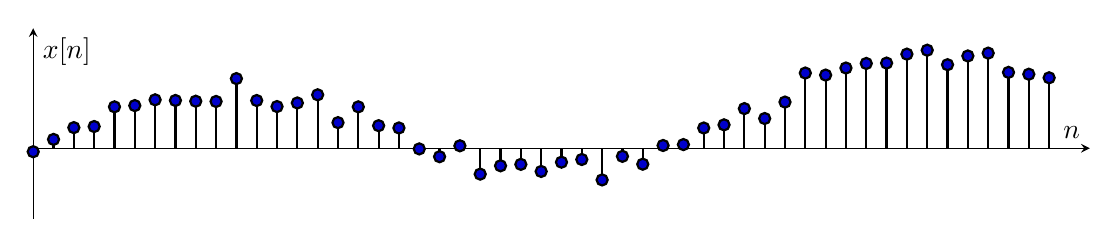
\begin{tikzpicture}
		\begin{axis}[%
		axis x line=middle,
		axis y line=middle,
		ticks=none,
		enlarge x limits=0,
		enlarge y limits=0.15,
		xmin=0,
		xmax=52,
		ymin=-1,
		width=15cm,
		height=4cm,
		domain = 0:50,
		samples = 51,
		xlabel={$n$},
		ylabel={$x[n]$}]
		\addplot+[ycomb,black,thick] {sin(2*180*x/35) + 0.3*rand + x/50 };
		\end{axis}
	\end{tikzpicture}
	\end{center}
    \begin{center}
	\huge{$\vdots$}
	\end{center}
	\begin{center}
	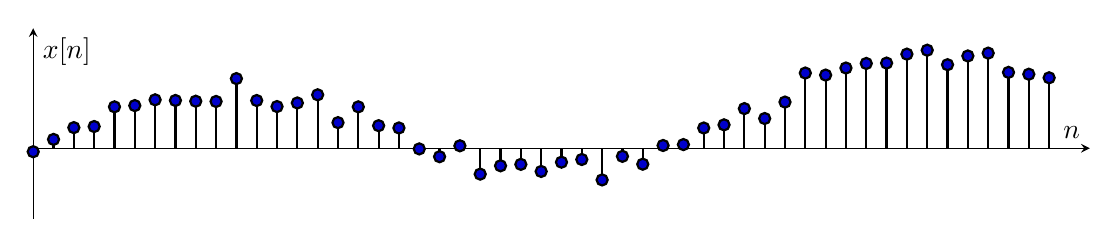
\begin{tikzpicture}
	\begin{axis}[%
		axis x line=middle,
		axis y line=middle,
		ticks=none,
		enlarge x limits=0,
		enlarge y limits=0.15,
		xmin=0,
		xmax=52,
		ymin=-1,
		width=15cm,
		height=4cm,
		domain = 0:50,
		samples = 51,
		xlabel={$n$},
		ylabel={$x[n]$}]
		\addplot+[ycomb,black,thick] {sin(2*180*x/35) + 0.3*rand + x/50};
\end{axis}
\end{tikzpicture}
	\end{center}
\caption{Realizations of a discrete stochastic process}
\label{fig:realizations_stochastic_process}
\end{figure}

\section{Preliminaries: Spectral analysis of deterministic signals}
\label{sec:preliminaries_deterministic_signals}
	
Before going into the spectral analysis of stochastic processes, it is convenient to study the case of deterministic signals, which will help us to understand the concept of spectral resolution. Thus, the problem is to compute the Fourier transform of the deterministic signal $x[n]$. However, this relatively ``simple'' task has two problems. First, we do not have access to the whole signal $x[n]$, but only to a finite record thereof
\begin{equation*}
   x_w[n]  = \begin{cases}
   x[n], & n = 0, \ldots, N-1, \\
   0, & \text{otherwise.}
   \end{cases}
\end{equation*}
Defining now the window
\begin{equation*}
w_{R,N}[n]  = \begin{cases}
1, & n = 0, \ldots, N-1, \\
0, & \text{otherwise,}
\end{cases}
\end{equation*}
we may rewrite $x_w[n] = w_{R,N}[n] x[n]$, which allows us to compute the Fourier transform of $x_w[n]$ as\footnote{In the ``Signals and Systems'' parlance, this Fourier transform is named Discrete Time Fourier Transform (DTFT).}
\begin{equation}
\label{eq:DTFT}
X_w(e^{j \omega}) = \mathcal{F} \left(x_w[n]\right) = \sum_{n = 0}^{N-1} x_w[n] e^{- j \omega N} = \frac{1}{2 \pi} W_{R,N}(e^{j \omega}) \circledast X(e^{j \omega}),
\end{equation}
where $\circledast$ denotes the circular convolution. So, the Fourier transform of the windowed signal, $x_w[n]$, is related to that of $x[n]$ through the Fourier transform of the window $w_{R,N}[n]$, which is given by
\begin{equation*}
W_{R,N}(e^{j \omega}) = e^{-j \omega (N-1)/2} \frac{\sin\left(\frac{\omega N}{2}\right)}{\sin\left(\frac{\omega}{2}\right)} = e^{-j \omega (N-1)/2} P_N(e^{j \omega}),
\end{equation*}
and its amplitude $|P_N(e^{j \omega})|$ is depicted in Figure \ref{fig:FT_rectangularwindow}. As this figure shows, the width of the main lobe is $4 \pi/N$.

\begin{figure}
	\pgfmathsetmacro{\mypi}{3.141592}
	\pgfmathsetmacro{\windowlength}{10}
	\begin{center}
		\begin{tikzpicture}
		\begin{axis}[%
		axis x line=middle,
		axis y line=middle,
		enlarge x limits=0.05,
		enlarge y limits=0.2,
		xtick={-\mypi,-2*\mypi/\windowlength,2*\mypi/\windowlength,\mypi},
		xticklabels={$-\pi$,$-\frac{2\pi}{N}$,$\frac{2\pi}{N}$,$\pi$},
		xmin=-\mypi,
		xmax=\mypi,
		ymin=0,
		ytick=\empty,
		width=10cm,
		height=7.5cm,
		domain = -\mypi:\mypi,
		samples = 512,
		xlabel={$\omega$},
		ylabel={$|P_N(e^{j \omega})|$}]
		%\addplot+[ycomb,black,thick] {x*\mypi};
		\addplot[black,thick] {abs(sin(deg(x*\windowlength/2))/sin(deg(x/2)))};
		\end{axis}
		\end{tikzpicture}
	\end{center}
	\caption{Module of the Fourier transform of the rectangular window}
	\label{fig:FT_rectangularwindow}
\end{figure}

The second issue is that the DTFT in \eqref{eq:DTFT} is a function of a continuous variable. Hence it cannot be computed nor stored in a computer. The solution is simple and consists in discretizing the spectrum, which yields the Discrete Fourier Transform (DFT). Thus, we are only able to compute $X_w(e^{j \omega_k}),$ with $\omega_k = 2 \pi k/N$ and $k = 0, \ldots, N-1$. The DFT is typically computed using the fast Fourier transform (FFT) algorithm. 

The aforementioned procedure based on the DFT/FFT gets only $N$ samples of the spectrum for length-$N$ signals, but we can get more samples by zero-padding the signals, i.e., by simply adding $N_\text{fft} - N$ zeros after the $N$ samples. This procedure increases the number of frequencies but it does not increase the resolution as it does not modify the window.
	
%%%%%%%%%%%%%%%
\begin{example}[Spectral analysis of a complex exponential]
	\label{ex:spectral_analysis_deterministic}
	
	This example considers the spectral analysis of a finite record of a complex exponential, i.e., $x[n] = e^{j \omega_0 n}, n = 0, \ldots, N-1$. Using the DTFT of a complex exponential, given by
\begin{equation*}
X(e^{j \omega}) = 2 \pi \delta(\omega - \omega_0),
\end{equation*}
and $W_N(e^{j \omega})$, $X_w(e^{j \omega})$ becomes
\begin{equation*}
X_w(e^{j \omega}) = e^{-j (\omega - \omega_0) (N-1)/2} \frac{\sin\left(\frac{(\omega - \omega_0) N}{2}\right)}{\sin\left(\frac{\omega - \omega_0}{2}\right)} =  e^{-j (\omega - \omega_0) (N-1)/2} P_N\left(\omega - \omega_0\right),
\end{equation*}
and its magnitude squared is
\begin{equation*}
|X_w(e^{j \omega})|^2 = \left|P_N\left(e^{j (\omega - \omega_0)}\right)\right|^2.
\end{equation*}
Figure \ref{fig:FT_complexexponential} plots, in logarithmic scale, $|X_w(e^{j \omega})|^2$ and $|X_w(e^{j \omega_k})|^2$ for two different values of $N_\text{fft}$.
\begin{figure}
	\pgfmathsetmacro{\mypi}{3.141592}
	\pgfmathsetmacro{\windowlength}{14}
	\pgfmathsetmacro{\myomega}{\mypi/8}
	\begin{center}
		\begin{tikzpicture}
		\begin{axis}[%
		axis x line=bottom,
		axis y line=middle,
		enlarge x limits=0.05,
		enlarge y limits=0.2,
		xtick={-\mypi,\myomega,\mypi},
		xticklabels={$-\pi$,$\omega_0$,$\pi$},
		xmin=-\mypi,
		xmax=\mypi,
		ymin=1e-3,
		ytick=\empty,
		ymode=log,
		width=8cm,
		height=6cm,
		domain = -\mypi:\mypi,
		samples = 512,
		xlabel={$\omega$},
		ylabel={$|X_w(e^{j \omega})|^2$}]
		%\addplot+[ycomb,black,thick] {x*\mypi};
		\addplot[black,thick] {(sin(deg((x-\myomega)*\windowlength/2))/sin(deg((x-\myomega)/2)))^2};
		\addplot+[only marks,mark=*,black,thick,each nth point=32] {(sin(deg((x-\myomega)*\windowlength/2))/sin(deg((x-\myomega)/2)))^2};
		\end{axis}
		\end{tikzpicture}
		\hspace{0.5cm}
		\begin{tikzpicture}
\begin{axis}[%
axis x line=bottom,
axis y line=middle,
enlarge x limits=0.05,
enlarge y limits=0.2,
xtick={-\mypi,\myomega,\mypi},
xticklabels={$-\pi$,$\omega_0$,$\pi$},
xmin=-\mypi,
xmax=\mypi,
ymin=1e-3,
ytick=\empty,
ymode=log,
width=8cm,
height=6cm,
domain = -\mypi:\mypi,
samples = 512,
xlabel={$\omega$},
ylabel={$|X_w(e^{j \omega})|^2$}]
\addplot[black,thick] {(sin(deg((x-\myomega)*\windowlength/2))/sin(deg((x-\myomega)/2)))^2};
\addplot+[only marks,mark=*,black,thick,each nth point=16] {(sin(deg((x-\myomega)*\windowlength/2))/sin(deg((x-\myomega)/2)))^2};
\end{axis}
\end{tikzpicture}
	\end{center}
	\caption{Fourier transform (in logarithmic scale) of a windowed complex exponential}
	\label{fig:FT_complexexponential}
\end{figure}
		
As we have seen in this example, the spectral analysis of deterministic signals depends on two factors. First, the number of available samples, which determines the window and, therefore, the shape of the windowed spectrum. As we have seen in Figure \ref{fig:FT_complexexponential}, the rectangular window has a narrow main lobe at the expense of high secondary lobes. This effect could be reduced by pre-multiplying $x_w[n]$ by a different window, which would reduce the height of the secondary lobes, but it would widen the main lobe.

\end{example}
%%%%%%%%%%%%%

%%%%%%%%%%%%%%%
\begin{example}[Spectral analysis of two complex exponentials]
	\label{ex:spectral_analysis_deterministic_two}
	
	This example considers the spectral analysis of a finite record of the sum of two complex exponential, i.e., $x[n] = e^{j \omega_0 n} + e^{j \omega_1 n}, n = 0, \ldots, N-1$, which will help us to understand the concept of resolution. Using \eqref{eq:DTFT}, we have
	\begin{equation*}
	X_w(e^{j \omega}) = e^{-j (\omega - \omega_0) (N-1)/2} P_N\left(\omega - \omega_0\right)+  e^{-j (\omega - \omega_1) (N-1)/2} P_N\left(\omega - \omega_1\right).
	\end{equation*}
	and its magnitude squared is
	\begin{multline*}
	|X_w(e^{j \omega})|^2 = \left|P_N\left(e^{j (\omega - \omega_0)}\right)\right|^2 + \left|P_N\left(e^{j (\omega - \omega_1)}\right)\right|^2  \\  + e^{j (\omega_0 - \omega_1) (N-1)/2} P_N\left(e^{j (\omega - \omega_0)}\right) P_N\left(e^{j (\omega - \omega_1)}\right)\\ +  e^{- j (\omega_0 - \omega_1) (N-1)/2} P_N\left(e^{j (\omega - \omega_0)}\right) P_N\left(e^{j (\omega - \omega_1)}\right).
\end{multline*}
Taking into account Euler's formula, $|X_w(e^{j \omega})|^2$ can be simplified as
	\begin{multline*}
|X_w(e^{j \omega})|^2 = \left|P_N\left(e^{j (\omega - \omega_0)}\right)\right|^2 + \left|P_N\left(e^{j (\omega - \omega_1)}\right)\right|^2  \\  + 2 \cos \left(\frac{(\omega_0 - \omega_1) (N-1)}{2} \right) P_N\left(e^{j (\omega - \omega_0)}\right) P_N\left(e^{j (\omega - \omega_1)}\right).
\end{multline*}
Figure \ref{fig:FT_twocomplexexponential} plots, in logarithmic scale, $|X_w(e^{j \omega})|^2$ for two different separations between the frequencies of the exponentials. As we can see in this figure, for small frequency separations, it is impossible to identify in the spectrum the two complex exponentials.
	\begin{figure}
		\pgfmathsetmacro{\mypi}{3.141592}
		\pgfmathsetmacro{\windowlength}{14}
		\pgfmathsetmacro{\myomega}{\mypi/8}
		\pgfmathsetmacro{\myomegabis}{3*\mypi/8}
		\pgfmathsetmacro{\myomegabisbis}{1.5*\mypi/8}
		\begin{center}
	\begin{tikzpicture}
\begin{axis}[%
axis x line=bottom,
axis y line=middle,
enlarge x limits=0.05,
enlarge y limits=0.2,
xtick={-\mypi,\myomega,\myomegabis,\mypi},
xticklabels={$-\pi$,$\omega_0$,$\omega_1$,$\pi$},
xmin=-\mypi,
xmax=\mypi,
ymin=1e-3,
ytick=\empty,
ymode=log,
width=8cm,
height=6cm,
domain = -\mypi:\mypi,
samples = 512,
xlabel={$\omega$},
ylabel={$|X_w(e^{j \omega})|^2$}]
\addplot[black,thick] {(sin(deg((x-\myomega)*\windowlength/2))/sin(deg((x-\myomega)/2)))^2 + (sin(deg((x-\myomegabis)*\windowlength/2))/sin(deg((x-\myomegabis)/2)))^2  + 2*cos(deg((\myomega - \myomegabis)*(\windowlength - 1)/2))*(sin(deg((x-\myomega)*\windowlength/2))/sin(deg((x-\myomega)/2)))*(sin(deg((x-\myomegabis)*\windowlength/2))/sin(deg((x-\myomegabis)/2)))};
\end{axis}
\end{tikzpicture}
	\begin{tikzpicture}
\begin{axis}[%
axis x line=bottom,
axis y line=middle,
enlarge x limits=0.05,
enlarge y limits=0.2,
xtick={-\mypi,\myomega,\mypi},
xticklabels={$-\pi$,$\omega_0$,$\pi$},
extra x ticks={\myomegabisbis},
extra x tick labels={$\omega_1$},
extra x tick style={tick label style={yshift=5mm}},
xmin=-\mypi,
xmax=\mypi,
ymin=1e-3,
ytick=\empty,
ymode=log,
width=8cm,
height=6cm,
domain = -\mypi:\mypi,
samples = 512,
xlabel={$\omega$},
ylabel={$|X_w(e^{j \omega})|^2$}]
\addplot[black,thick] {(sin(deg((x-\myomega)*\windowlength/2))/sin(deg((x-\myomega)/2)))^2 + (sin(deg((x-\myomegabisbis)*\windowlength/2))/sin(deg((x-\myomegabisbis)/2)))^2  + 2*cos(deg((\myomega - \myomegabisbis)*(\windowlength - 1)/2))*(sin(deg((x-\myomega)*\windowlength/2))/sin(deg((x-\myomega)/2)))*(sin(deg((x-\myomegabisbis)*\windowlength/2))/sin(deg((x-\myomegabisbis)/2)))};
\end{axis}
\end{tikzpicture}
		\end{center}
		\caption{Fourier transform (in logarithmic scale) of the sum of two complex exponentials}
		\label{fig:FT_twocomplexexponential}
	\end{figure}
	
\end{example}
%%%%%%%%%%%%%

\section{Non-parametric methods in spectral estimation}

In this section, we turn our attention to the case of stochastic signals and, in particular, to the development of non-parametric spectral estimation methods. We will therefore study the periodogram and variations thereof. 

Before proceeding, let us note that throughout this section, we will only consider DTFTs. However, we have to keep in mind that, in practice, we can only compute the DFT (using the FFT algorithm), as we have seen in Section \ref{sec:preliminaries_deterministic_signals}.

\subsection{The periodogram}

Despite the title section, we will start with an estimator known as correlogram, which is based on a first definition of the PSD.
\begin{definition}
	\label{wiener_khinchin}
	Given a WSS process $x[n]$, the power spectral density is defined as
	\begin{equation*}
	S_x(e^{j \omega}) = \mathcal{F}(r_{x}[m]),
	\end{equation*}
	where
	\begin{equation*}
	r_{x}[m] = \mathbb{E}[x[n] x^{\ast}[n-m]],
	\end{equation*}
	is the auto-correlation function of the process $x[n]$.
\end{definition}

Based on Definition \ref{wiener_khinchin}, the first estimator of the PSD is given by
\begin{equation*}
	\hat{S}_x(e^{j \omega}) = \mathcal{F}(\hat{r}_{x}[m]),
\end{equation*}
where $\hat{r}_{x}[m]$ is an estimator of the auto-correlation function. Concretely, we have two alternatives for this estimator: a biased and an unbiased estimator. The biased estimator of the auto-correlation, given the finite length $x[n], n = 0, \ldots, N-1$, is
\begin{equation}
	\label{eq:autocorrelation_biased}
	\hat{r}_{x}^{b}[m] = \frac{1}{N} \sum_{n = m}^{N-1} x[n] x^{\ast}[n-m], \quad m = 0, \ldots, N-1,
\end{equation}
and $\hat{r}_{x}^{b}[m] = \left[ \hat{r}_{x}^{b}[-m] \right]^{\ast}, m = -N+1, \ldots, -1$, whereas the unbiased estimator is
\begin{equation}
	\label{eq:autocorrelation_unbiased}
\hat{r}_{x}^{u}[m] = \frac{1}{N-m} \sum_{n = m}^{N-1} x[n] x^{\ast}[n-m], \quad m = 0, \ldots, N-1,
\end{equation}
and $\hat{r}_{x}^{u}[m] = \left[ \hat{r}_{x}^{u}[-m] \right]^{\ast}, m = -N+1, \ldots, -1$. Consequently, the PSD estimators are
\begin{equation}
\label{eq:correlogram}
\hat{S}_x^{b}(e^{j \omega}) = \mathcal{F}(\hat{r}_{x}^{b}[m]),
\end{equation}
and
\begin{equation*}
\hat{S}_x^{u}(e^{j \omega}) = \mathcal{F}(\hat{r}_{x}^{u}[m]).
\end{equation*}
Actually, only the estimator in \eqref{eq:correlogram}, which is known as the correlogram, is a valid PSD estimator since it ensures $\hat{S}_x^{b}(e^{j \omega}) \geq 0$, whereas $\hat{S}_x^{u}(e^{j \omega}) \not \geq 0$.

The periodogram, which is a term coined by Arthur Schuster in 1898, is based on a second definition of the power spectral density. This definition states that
\begin{equation*}
	S_x(e^{j \omega}) = \lim_{N \rightarrow \infty} \ E \left[\frac{1}{2N -1} \left| \sum_{n = -N+1}^{N-1} x[n] e^{-j \omega n} \right|^2 \right].
\end{equation*}
The periodogram is obtained from the above definition by simply dropping the expectation and considering a finite number of samples, i.e.,
\begin{equation}
	\label{eq:periodogram}
	\hat{S}_x^{p}(e^{j \omega}) = \frac{1}{N} \left| \sum_{n = 0}^{N-1} x[n] e^{-j \omega n} \right|^2 = \frac{1}{N} \left| X(e^{j \omega}) \right|^2,
\end{equation}
where $X(e^{j \omega})  = \mathcal{F}(x[n])$.

In the following, we will shed some light on why we have started this section with the correlogram. Let us start by rewriting $\hat{r}_{x}^{b}[m]$ as
\begin{equation*}
\hat{r}_{x}^{b}[m] = \frac{1}{N} \sum_{n = m}^{N-1} x[n] x^{\ast}[n-m] = \frac{1}{N} \sum_{n = -\infty}^{\infty} x[n] x^{\ast}[n-m]  = \frac{1}{N} \left(x[n] \ast x^{\ast}[-n]\right),
\end{equation*}
and taking its Fourier transform yields
\begin{equation*}
\hat{S}_x^{b}(e^{j \omega}) = \mathcal{F}(\hat{r}_{x}^{b}[m]) = \frac{1}{N} \mathcal{F} \left(x[n] \ast x^{\ast}[-n]\right).
\end{equation*}
Finally, applying the properties of the Fourier transform, $\hat{S}_x^{b}(e^{j \omega})$ simplifies to
\begin{equation*}
\hat{S}_x^{b}(e^{j \omega}) = \frac{1}{N} \mathcal{F} \left(x[n] \right) \mathcal{F} \left(x^{\ast}[-n]\right) = \frac{1}{N} X(e^{j \omega}) X^{\ast}(e^{j \omega}) = \frac{1}{N} \left| X(e^{j \omega}) \right|^2 = \hat{S}_x^{p}(e^{j \omega}),
\end{equation*}
which is the periodogram in \eqref{eq:periodogram}. That is, the periodogram and the correlogram are identical.

\subsubsection{Bias and variance of the periodogram}

To understand why we need more refined estimators of the power spectral density, now we shall perform the statistical analysis of the periodogram (or correlogram), i.e.,  we will compute its bias and variance as we would do with any other estimator.

The first question is whether the periodogram is a biased estimator of the PSD, that is, 
\begin{equation*}
E\left[\hat{S}_x^{p}(e^{j \omega}) \right] \mathop{=}^{?} S_x(e^{j \omega}).
\end{equation*}
To compute the bias of the periodogram, it is easier to consider the equivalence with the correlogram, which allows us to write
\begin{equation*}
E\left[\hat{S}_x^{p}(e^{j \omega}) \right] = E\left[\mathcal{F}(\hat{r}_{x}^{b}[m]) \right] = \mathcal{F}\left(E\left[ \hat{r}_{x}^{b}[m]\right]\right),  
\end{equation*}
where we have used that the expectation and the Fourier transform are both linear operators. Thus, the periodogram is biased if $\hat{r}_{x}^{b}[m]$ is a biased estimate of the auto-correlation function. Now, using the definition of  $\hat{r}_{x}^{b}[m]$, we get\footnote{It is easy to prove that $\hat{r}_{x}^{u}[m]$ is indeed an unbiased estimate of the auto-correlation function, which is left as an exercise for the student.}
\begin{multline*}
E\left[ \hat{r}_{x}^{b}[m]\right] = E\left[ \frac{1}{N} \sum_{n = m}^{N-1} x[n] x^{\ast}[n-m] \right] = \frac{1}{N} \sum_{n = m}^{N-1} E\left[ x[n] x^{\ast}[n-m] \right] \\ = \frac{1}{N} \sum_{n = m}^{N-1} r_{x}[m] = \frac{N - |m|}{N} r_{x}[m] \neq r_{x}[m],
\end{multline*}
which shows that $\hat{r}_{x}^{b}[m]$ is indeed a biased estimate of the auto-correlation function, with the exception of $m = 0$, and makes the periodogram a biased estimate of the PSD.

It is possible to obtain a closed-form expression for the bias of the periodogram by noting that
\begin{equation}
\label{eq:bias_auto-correlation}
E\left[\hat{r}_{x}^{b}[m]\right]  = \frac{N - |m|}{N} r_{x}[m] = w_{T,N}[m] r_{x}[m],
\end{equation}
where the triangular, or Barlett window, is defined as
\begin{equation*}
w_{T,N}[m] = \begin{cases} \frac{N - |m|}{N}, & |m| \leq N-1, \\
0, & \text{otherwise},
\end{cases}
\end{equation*}
and is depicted in Figure \ref{fig:triangularwindow}. The bias given in \eqref{eq:bias_auto-correlation} shows us that the larger the $m$ the larger the bias.
\begin{figure}
	\pgfmathsetmacro{\windowlength}{10}
	\begin{center}
		\begin{tikzpicture}
		\begin{axis}[%
		axis x line=middle,
		axis y line=middle,
		ticks=none,
		enlarge x limits=0.1,
		enlarge y limits=0.15,
		xmin=-\windowlength,
		xmax=\windowlength,
		ymin=0,
		ymax=1.2,
		width=10cm,
		height=7.5cm,
		domain = -\windowlength:\windowlength,
		samples = 2*\windowlength + 1,
		xlabel={$m$},
		ylabel={$w_{T,N}[m]$}]
		\addplot+[ycomb,black,thick] {(\windowlength - abs(x))/\windowlength};
		\end{axis}
		\end{tikzpicture}
	\end{center}
	\caption{Triangular window}
	\label{fig:triangularwindow}
\end{figure}


Using \eqref{eq:bias_auto-correlation}, the bias of the periodogram becomes
\begin{equation}
\label{eq:bias_periodogram}
E\left[\hat{S}_x^{p}(e^{j \omega}) \right] = \mathcal{F}\left(w_{T,N}[m] r_{x}[m]\right) = \frac{1}{2 \pi} W_{T,N}(e^{j \omega}) \circledast S_x(e^{j \omega}),
\end{equation}
where
\begin{align*}
W_{T,N}(e^{j \omega}) &= \mathcal{F}\left(w_{T,N}[m]\right) = \frac{1}{N} \mathcal{F}\left(w_{R,N}[m] \ast w_{R,N}[-m]\right) = |W_{R,N}(e^{j \omega})|^2 \nonumber  \\  &= \frac{1}{N} \frac{\sin^2\left(\frac{\omega N}{2}\right)}{\sin^2\left(\frac{\omega}{2}\right)},
\end{align*}
is the Fourier transform of the triangular window and is depicted in Figure \ref{fig:FT_triangularwindow}. Comparing Figures \ref{fig:FT_rectangularwindow} and \ref{fig:FT_triangularwindow}, it can be seen that the level of secondary lobes is smaller for the triangular window. By analogy with Example \ref{ex:spectral_analysis_deterministic_two}, we can say that the bias of the periodogram is related with its resolution.

\begin{figure}
	\pgfmathsetmacro{\mypi}{3.141592}
	\pgfmathsetmacro{\windowlength}{10}
	\begin{center}
		\begin{tikzpicture}
		\begin{axis}[%
		axis x line=middle,
		axis y line=middle,
		enlarge x limits=0.05,
		enlarge y limits=0.2,
		xtick={-\mypi,-2*\mypi/\windowlength,2*\mypi/\windowlength,\mypi},
		xticklabels={$-\pi$,$-\frac{2\pi}{N}$,$\frac{2\pi}{N}$,$\pi$},
		xmin=-\mypi,
		xmax=\mypi,
		ymin=0,
		ytick=\empty,
		width=10cm,
		height=7.5cm,
		domain = -\mypi:\mypi,
		samples = 512,
		xlabel={$\omega$},
		ylabel={$W_{T,N}(e^{j \omega})$}]
		\addplot[black,thick] {(sin(deg(x*\windowlength/2))/sin(deg(x/2)))^2};
		\end{axis}
		\end{tikzpicture}
	\end{center}
	\caption{Fourier transform of the triangular window}
	\label{fig:FT_triangularwindow}
\end{figure}

We have shown in \eqref{eq:bias_periodogram} that the periodogram is biased. However, there are some cases when it is not. For instance, considering the asymptotic regime, it is unbiased:
\begin{equation*}
\lim_{N \rightarrow \infty} \hat{S}_x^{p}(e^{j \omega}) = S_x(e^{j \omega}).
\end{equation*}
Another case is when the process $x[n]$ is white noise. For this kind of processes, $r_{x}[m] = \sigma^2_x \delta[m]$ and, therefore
\begin{equation*}
E\left[\hat{r}_{x}^{b}[m]\right]  = \frac{N - |m|}{N} r_{x}[m] = \sigma^2_x \delta[m] = r_{x}[m].
\end{equation*}
Since the estimate of the auto-correlation is unbiased for white processes, it is easy to show that the periodogram is also unbiased.

The analysis of the variance of the periodogram is cumbersome and can only be done in particular cases. For white noise, it can be shown that
\begin{equation*}
 \mathop{Var}\left(\hat{S}_x^{p}(e^{j \omega})\right) = S_x^{2}(e^{j \omega}),
\end{equation*}
and in general we can say that
\begin{equation*}
\mathop{Var}\left(\hat{S}_x^{p}(e^{j \omega})\right) \appropto S_x^{2}(e^{j \omega}),
\end{equation*}
where $\appropto$ denotes approximately proportional to.  This expression tells us that the variance does not decrease for larger data records. That is, the periodogram is not a consistent estimate of the PSD.

\subsection{The Blackman-Tukey estimator}

One of the reasons for the behavior of the periodogram variance is the poor quality of the estimate $\hat{r}_{x}^{b}[m]$ for values of $m$ close to $N$. This problem is what the Blackman-Tukey (BT) estimator tries to improve. The idea is to ignore or weight the samples of $\hat{r}_{x}^{b}[m]$ for $m$ close to $N$. Thus, the BT estimator is
\begin{equation}
\label{eq:BT_definition}
\hat{S}_x^{BT}(e^{j \omega}) = \mathcal{F}(w_M[m] \hat{r}_{x}^{b}[m]) = \sum_{m = -N + 1}^{N-1} w_M[m] \hat{r}_{x}^{b}[m] e^{-j \omega m},
\end{equation}
where $w[m]$ is a window that must fulfill
\begin{equation*}
w_{M}[m] = \begin{cases} f(|m|), & |m| \leq M-1, \\
0, & \text{otherwise},
\end{cases}
\end{equation*}
where $f(|m|)$ is a monotonically decreasing function of $|m|$ and $M \leq N$. This window ignores the lags of the estimated auto-correlation for $|m|>M-1$ and weights  the lags for large $m$. The choice of the window  is critical to achieve good performance, but, in any case, it must guarantee that $\hat{S}_x^{BT}(e^{j \omega}) \geq 0$.

Using the properties of the Fourier transform, we may rewrite $\hat{S}_x^{BT}(e^{j \omega})$ as
\begin{equation*}
\hat{S}_x^{BT}(e^{j \omega}) = \frac{1}{2 \pi} W_M(e^{j \omega}) \circledast \hat{S}_x^{p}(e^{j \omega}) = \frac{1}{2 \pi} \int_{-\pi}^{\pi} W_{M}(e^{j \psi}) \hat{S}_x^{p}(e^{j (\omega - \psi)}) d \psi,
\end{equation*} 
where $W_M(e^{j \omega}) = \mathcal{F}(w_M[n])$. Then, the Blackman-Tukey estimator is locally smoothing the periodogram, which reduces its variance. However, there is no free lunch and we will show that this variance reduction translates into lower resolution (or larger bias). Concretely, the bias of the BT estimator is
\begin{equation*}
E\left[\hat{S}_x^{BT}(e^{j \omega})\right] = \frac{1}{2 \pi} W_M(e^{j \omega}) \circledast E\left[\hat{S}_x^{p}(e^{j \omega})\right] = \frac{1}{2 \pi} W_M(e^{j \omega}) \circledast  W_{T,N}(e^{j \omega}) \circledast S_x(e^{j \omega}).
\end{equation*}
Finally, since $w_M[n]$ is shorter than $w_{T,N}[n]$, it can be shown that $W_M(e^{j \omega})$ is wider than $W_{T,M}(e^{j \omega})$, which translates into a lower resolution. This behavior is depicted in Figure \ref{fig:comparison_windows} for $w_M[n] = w_{T,M}[n]$. Note that the $y$-axis is in logarithmic scale.
\begin{figure}
	\pgfmathsetmacro{\mypi}{3.141592}
	\pgfmathsetmacro{\windowlength}{10}
	\pgfmathsetmacro{\windowlengthbis}{6}
	\begin{center}
		\begin{tikzpicture}
		\begin{axis}[%
		axis x line=bottom,
		axis y line=middle,
		enlarge x limits=0.05,
		enlarge y limits=0.2,
		xtick={-\mypi,-2*\mypi/\windowlengthbis,-2*\mypi/\windowlength,2*\mypi/\windowlength, 2*\mypi/\windowlengthbis,\mypi},
		xticklabels={$-\pi$,$-\frac{2\pi}{M}$,$-\frac{2\pi}{N}$,$\frac{2\pi}{N}$,$\frac{2\pi}{M}$,$\pi$},
		xmin=-\mypi,
		xmax=\mypi,
		ymin=1e-3,
		ymode=log,
		ytick=\empty,
		width=10cm,
		height=7.5cm,
		domain = -\mypi:\mypi,
		samples = 512,
		xlabel={$\omega$}]
		\addplot[black,thick] {(sin(deg(x*\windowlength/2))/sin(deg(x/2)))^2};
		\addplot[blue,thick] {2.8*(sin(deg(x*\windowlengthbis/2))/sin(deg(x/2)))^2};
		\legend{$W_{T,N}(e^{j \omega})$,$W_{T,M}(e^{j \omega})$};
		\end{axis}
		\end{tikzpicture}
	\end{center}
	\caption{Fourier transform (in logarithmic scale) of two triangular windows of different lengths}
	\label{fig:comparison_windows}
\end{figure}

\subsection{Estimators based on the averaged periodogram}

The Blackman-Tukey estimator yields a smaller variance than that of the periodogram because, as we have seen, it smooths the periodogram. An alternative to reduce the variance is to average several periodograms. However, the question is: How do we obtain such periodograms? The answer is easy and consists in dividing the $N$ observations into windows of length $M < N$. 

The Barlett method is one of the possible estimators based on the averaged periodogram. First, it divides the $N$ observations into $L$ non-overlapping windows of length $M$ as
\begin{equation*}
	x_l[n] = x[(l-1) M + n],
\end{equation*}
where $n = 0, \ldots, M-1,$ and $l = 1, \ldots, L$, and computes the periodogram of each window, that is,
\begin{equation*}
\hat{S}_{x,l}^{p}(e^{j \omega}) = \frac{1}{M} \left| \sum_{n = 0}^{M-1} x_l[n] e^{-j \omega n} \right|^2 = \frac{1}{M} \left| X_l(e^{j \omega}) \right|^2.
\end{equation*}
Then, the Barlett estimator is given by simply averaging the individual periodograms
\begin{equation*}
\hat{S}_{x}^{B}(e^{j \omega}) = \frac{1}{L} \sum_{l = 1}^{L}\hat{S}_{x,l}^{p}(e^{j \omega}).
\end{equation*}
Although it is out of the scope of these notes, we must point out that $\hat{S}_{x}^{B}(e^{j \omega})$ is somehow related to $\hat{S}_{x}^{BT}(e^{j \omega})$.

There are two further improvements of the periodogram. The first one is based on the Barlett estimator but substituting the individual periodograms by Blackman-Tukey estimates. The second one is based on dividing the $N$ observations into $L$ overlapping windows. The combination of both improvements is known as the Welch method.

One final question remains: What happens to the bias and variance of these methods. Regarding the bias (resolution), it is going to be smaller than that of the periodogram since $M < N$, as also happened to the Blackman-Tukey estimate. As for the variance, it is going to be reduced by a factor of $L$, the number of windows. That is,
\begin{equation*}
\mathop{Var}\left(\hat{S}_x^{ap}(e^{j \omega})\right) \approx \frac{1}{L} \mathop{Var}\left(\hat{S}_x^{p}(e^{j \omega})\right),
\end{equation*}
where $\hat{S}_x^{ap}(e^{j \omega})$ is any averaged periodogram (either Barlett or Welch methods) and $\approx$ is due to the non-independence between the windows. It would be an equality when the windows are independent, i.e., the Barlett method.

\section{Parametric methods in spectral estimation}

The problem of non-parametric methods is that they estimate an infinite number of parameters (the PSD at each frequency) from a sequence of $N$ observations. Clearly, this is an ill-posed problem since there are (many) more parameters to estimate than observations. To overcome this issue, we could postulate a parametric model for the PSD and estimate only the parameters of such model using the $N$ observations. For instance, the model could be $S_x(e^{j \omega})  = a + b \cos^2(\omega)$ and, hence, we only have to estimate $a$ and $b$.

Parametric approaches, as described above, can provide a significant performance boost if the signal fits the postulated model, otherwise the performance could be even worse than that of non-parametric methods. It is therefore of the utmost importance to select the proper model.

\subsection{Rational models for parametric spectral estimation}

These models consider a white Gaussian noise $u[n]$ with zero mean and variance $\sigma^2$ that goes through a causal and stable filter\footnote{A filter is said to be causal and stable if and only if all its poles are inside the unit circle.} $h[n]$ that has the following Fourier transform
\begin{equation*}
	H(e^{j \omega}) = \frac{B(e^{j \omega})}{A(e^{j \omega})} = \frac{\displaystyle \sum_{k = 0}^{q} b_k e^{-j \omega k}}{\displaystyle 1 + \sum_{k = 1}^{p} a_k e^{-j \omega k}},
\end{equation*}
which implies that
\begin{equation}
	\label{eq:signal_model_ARMA}
	x[n] = u[n] \ast h[n] = - \sum_{k = 1}^{p} a_k x[n -k] + \sum_{k = 0}^{q} b_k u[n-k].
\end{equation}
For these models, the PSD  is given by
\begin{equation}
\label{eq:PSD_ARMA}
S_x(e^{j \omega}) = S_u(e^{j \omega}) |H(e^{j \omega})|^2 = \sigma^2 \left|\frac{\displaystyle \sum_{k = 0}^{q} b_k e^{-j \omega k}}{\displaystyle 1 + \sum_{k = 1}^{p} a_k e^{-j \omega k}}\right|^2,
\end{equation}
and we only have to estimate $\sigma^2$, $a_1, \ldots, a_p$, and $b_0, \ldots, b_q$. 

According to Weierstrass theorem, for large values $p$ and $q$, the PSD model in \eqref{eq:PSD_ARMA} can approximate arbitrarily close any continuous PSD. Hence, there is a strong interest in this kind of models, which are named as auto-regressive moving average (ARMA or ARMA(p,q)). There are two special cases of the ARMA model that are particularly interesting: the auto-regressive (AR or AR(p)) and the moving average (MA or MA(q)). For the former, the PSD is given by
\begin{equation*}
S_x(e^{j \omega}) = \frac{\sigma^2}{\displaystyle \left|1 + \sum_{k = 1}^{p} a_k e^{-j \omega k}\right|^2},
\end{equation*}
whereas, for the latter, it is
\begin{equation*}
S_x(e^{j \omega}) =  \sigma^2 \left|\sum_{k = 0}^{q} b_k e^{-j \omega k}\right|^2.
\end{equation*}
AR models are good choices if we suspect the PSD has large peaks and MA models are good choices for PSDs with large valleys.

The estimation of the model parameters is typically carried out in the time domain, for which the auto-correlation structure is required. Once the auto-correlation function is available, which will depend in general on the model parameters in a non-linear fashion, the estimation procedure consists in substituting the theoretical auto-correlation by an estimate and then solving a non-linear system of equations. The PSD estimate is obtained by substituting the estimated parameters in the corresponding model. This procedure, which is conceptually simple, is actually rather involved. However, there is an exception, which is the AR model since the dependency of auto-correlation on the parameters is linear.

\subsection{The auto-correlation function of ARMA processes}

This section computes the auto-correlation function of ARMA processes, which is defined as
\begin{equation*}
	r_{x}[m] = \mathbb{E}[x[n] x^{\ast}[n-m]].
\end{equation*}
Substituting $x[n]$ by \eqref{eq:signal_model_ARMA}, $r_{x}[m]$ becomes
\begin{align*}
r_{x}[m] &= E\left[ \left(- \sum_{k = 1}^{p} a_k x[n -k]  + \sum_{k = 0}^{q} b_k u[n-k] \right) x^{\ast}[n-m]\right] \nonumber \\
&=  - \sum_{k = 1}^{p} a_k E\left[x[n -k] x^{\ast}[n-m]\right] + \sum_{k = 0}^{q} b_k  E\left[u[n-k]  x^{\ast}[n-m]\right] \nonumber \\
&=  - \sum_{k = 1}^{p} a_k r_{x}[m-k] + \sum_{k = 0}^{q} b_k  r_{ux}[m-k].
\end{align*}
where the cross-correlation function between $u[n]$ and $x[n]$ is
\begin{equation*}
r_{ux}[m] =   E\left[u[n]  x^{\ast}[n-m]\right].
\end{equation*}
Now, taking into account that
\begin{equation*}
x[n] = u[n] \ast h[n] = \sum_{l = -\infty}^{\infty} h[l] u[n-l],
\end{equation*}
the cross-correlation function becomes
\begin{align*}
r_{ux}[m] &=   E\left[u[n]  \sum_{l = -\infty}^{\infty} h^{\ast}[l] u^{\ast}[n-m-l]\right] \nonumber \\
&=   \sum_{l = -\infty}^{\infty} h^{\ast}[l] E\left[u[n]   u^{\ast}[n-m-l]\right] \nonumber \\
&=   \sum_{l = -\infty}^{\infty} h^{\ast}[l] r_u [m+l], \nonumber \\
&=   \sum_{l = -\infty}^{\infty} h^{\ast}[-l] r_u [m-l], \nonumber \\
&=   r_u [m] \ast h^{\ast}[-m],
\end{align*}
where the auto-correlation of $u[n]$ is
\begin{equation*}
r_{u}[m] = \mathbb{E}[u[n] u^{\ast}[n-m]] = \sigma^2 \delta[m],
\end{equation*}
because it is a white process. Then, $r_{ux}[m]$ simplifies to
\begin{equation*}
r_{ux}[m] =  \sigma^2 h^{\ast}[-m],
\end{equation*}
and plugging $r_{ux}[m]$ into $r_{x}[m]$, the desired auto-correlation becomes
\begin{equation*}
r_{x}[m] =  - \sum_{k = 1}^{p} a_k r_{x}[m-k] + \sigma^2 \sum_{k = 0}^{q} b_k  h^{\ast}[k-m].
\end{equation*}
The second term in the right-hand side of the the above equation can be expanded as
\begin{equation*}
\sigma^2 \sum_{k = 0}^{q} b_k  h^{\ast}[k-m] = \sigma^2  \left(b_0 h[-m] + b_1 h[1-m] + \ldots + b_q h[q-m]\right),
\end{equation*}
and since the filter is causal ($h[m] = 0, \forall m<0$), it becomes
\begin{align*}
\sigma^2  \sum_{k = 0}^{q} b_k  h^{\ast}[k-m] &= \begin{cases}
\sigma^2  \left(b_m h[0] + b_{m+1} h[1] + \ldots + b_q h[q-m]\right), & 0 \leq  m \leq q, \\ 
0, & m > q,
\end{cases} \nonumber \\
&= \begin{cases}
\displaystyle \sigma^2  \sum_{k = m}^{q} b_k  h^{\ast}[k-m], & 0 \leq  m \leq q, \\ 
0, & m > q.
\end{cases}
\end{align*}
Putting all pieces together we get
\begin{equation}
\label{eq:correlation_ARMA}
r_{x}[m] = \begin{cases}
\displaystyle - \sum_{k = 1}^{p} a_k r_{x}[m-k] + \sigma^2  \sum_{k = m}^{q} b_k  h^{\ast}[k-m], & 0 \leq  m \leq q, \\ 
\displaystyle  - \sum_{k = 1}^{p} a_k r_{x}[m-k], & m > q, \\
r_{x}^{\ast}[-m], & m < 0.
\end{cases}
\end{equation}
Keeping in mind that $h[m]$ will depend on $a_1, \ldots, a_p$, and $b_0, \ldots, b_q$, it is easy to see in \eqref{eq:correlation_ARMA} that the relationship between the model parameters ($\sigma^2$, $a_1, \ldots, a_p$, and $b_0, \ldots, b_q$) and the auto-correlation is non-linear, which complicates tremendously the estimation of such parameters from an estimate of the auto-correlation function. This is shown in the following example for a particular ARMA model.

\begin{example}[Auto-correlation function of an ARMA(1,1) process]
	
In this example, we will consider an ARMA(1,1) process, which has the following frequency response
\begin{equation*}
H(e^{j \omega}) = \frac{1 - b e^{-j \omega}}{1 - a e^{-j \omega}},
\end{equation*}
and the corresponding impulse response is
\begin{equation*}
h[n] = a^n s[n] - b a^{n-1} s[n-1],
\end{equation*}
where
\begin{equation*}
s[n] = \begin{cases}
1, & n \geq 0, \\
0, & n < 0.
\end{cases}
\end{equation*}
Now, we specialize \eqref{eq:correlation_ARMA} for the case of $p = 1, q = 1, b_0 = 1, b_1 = -b,$ and $a_1 = -a$, which yields
\begin{align*}
	r_x[0] &= a r_x[-1]  + \sigma^2 \left(1 + (-b) (a-b)^{\ast}\right), \\
	r_x[1] &= a r_x[0]  + \sigma^2  (-b), \\
	r_x[2] &= a r_x[1] , \\
	r_x[3] &= a r_x[2] , \\
	&\phantom{=} \vdots
\end{align*}
where we have taken into account that $h[0] = 1$ and $h[1] = a - b$. To recover the three model parameters, we need three equations, which are
\begin{equation*}
	\begin{bmatrix}
	r_x[0] & r_x[-1] \\
	r_x[1] & r_x[0] \\
	r_x[2] & r_x[1] 
	\end{bmatrix}
	\begin{bmatrix}
	1 \\ -a
	\end{bmatrix} = 
	\begin{bmatrix}
	\sigma^2 \left(1 - b (a-b)^{\ast}\right) \\
	\sigma^2  (-b) \\
	0
	\end{bmatrix}.
\end{equation*}
The first issue to solve the above system of equations is that we do not know $r_x[m]$, but as explained before it can be substituted by any estimator of the auto-correlation function, such as \eqref{eq:autocorrelation_biased} or \eqref{eq:autocorrelation_unbiased}, yielding
\begin{equation*}
	\begin{bmatrix}
	\hat{r}_x[0] & \hat{r}_x^{\ast}[1] \\
	\hat{r}_x[1] & \hat{r}_x[0] \\
	\hat{r}_x[2] & \hat{r}_x[1] 
\end{bmatrix}
\begin{bmatrix}
	1 \\ -a
\end{bmatrix} = 
\begin{bmatrix}
	\sigma^2 \left(1 - b (a-b)^{\ast}\right) \\
	\sigma^2  (-b) \\
	0
\end{bmatrix},
\end{equation*}
where we have used $\hat{r}_x[-1] = \hat{r}_x^{\ast}[1]$. The second issue is that the system of equations is non-linear, which makes it difficult to solve, even for this simple ARMA model.
\end{example}

\subsection{AR processes}

In the following, we will consider AR (= ARMA(p,0)) processes, which are the most commonly used ones among the three kind of processes studied in this course. There are several reasons. The first one is that the estimation of the parameters is much simpler. Actually, it can be done by simply solving a system of equations. Moreover, from the expression of an AR model
\begin{equation*}
x[n]  = u[n] - \sum_{k = 1}^{p} a_k x[n -k],
\end{equation*}
where we have assumed without loss of generality that $b_0 = 1$, we note that they can be used to predict future samples by ignoring the input, i.e.,
\begin{equation*}
x[n]  =  - \sum_{k = 1}^{p} \hat{a}_k x[n -k],
\end{equation*}
where the coefficient of the model have been replaced by some estimates. That is, from a record of $N$ samples, $x[0], \ldots, x[N-1]$, we can estimate the model parameters and, afterwards, we can predict $x[N], x[N+1], \ldots$

Let's now turn our attention to the estimation of the AR model parameters. Before proceeding, we shall require the impulse response of the system, which is given by
\begin{equation*}
h[n] = \left.x[n]\right|_{u[n] = \delta[n]} = \delta[n] - \sum_{k = 1}^{p} a_k h[n -k],
\end{equation*}
and since the filter is causal, we find that $h[0] = 1$, and allows us to particularize \eqref{eq:correlation_ARMA} as follows
\begin{equation}
\label{eq:correlation_AR}
r_{x}[m] = \begin{cases}
\displaystyle - \sum_{k = 1}^{p} a_k r_{x}[m-k] + \sigma^2  \overbrace{h^{\ast}[0]}^1, & m = 0, \\ 
\displaystyle  - \sum_{k = 1}^{p} a_k r_{x}[m-k], & m > 0, \\
r_{x}^{\ast}[-m], & m < 0.
\end{cases}
\end{equation}
Equation \eqref{eq:correlation_AR} shows that the auto-correlation function of the AR model does not depend on $h[n]$, which is the term that introduces non-linear relationships. Since we need to obtain $p+1$ parameters, i.e., $a_1, \ldots, a_p$ and $\sigma^2$, we need $p+1$ equations, which are
\begin{align*}
r_x[0] &= -a_1 r_x[-1] - a_2 r_x[-2] + \ldots -a_p r_x[-p] + \sigma^2, \\
r_x[1] &= -a_1 r_x[0] - a_2 r_x[-1] + \ldots -a_p r_x[-p+1], \\
r_x[2] &= -a_1 r_x[1] - a_2 r_x[0] + \ldots -a_p r_x[-p+2], \\
	&\phantom{=} \vdots \\
r_x[p] &= -a_1 r_x[p-1] - a_2 r_x[p-2] + \ldots -a_p r_x[0].
\end{align*}
The last $p$ equations depend only on $a_1, \ldots, a_p$. Writing them in matrix form, we get
\begin{equation*}
\begin{bmatrix}
r_x[0] & r_x[-1] & \cdots & r_x[-p+1] \\
r_x[1] & r_x[0] & \cdots & r_x[-p+2] \\
\vdots & \vdots & \ddots & \vdots \\
r_x[p-1] & r_x[p-2] & \cdots & r_x[0] 
\end{bmatrix}
\begin{bmatrix}
-a_1 \\ -a_2 \\ \vdots \\ -a_p
\end{bmatrix} = 
\begin{bmatrix}
r_x[1] \\ r_x[2] \\ \vdots \\ r_x[p]
\end{bmatrix},
\end{equation*}
which are known as the Yule-Walker equations. Hence, the filter coefficients are obtained by solving a linear system of equations
\begin{equation*}
\begin{bmatrix}
\hat{a}_1 \\ \hat{a}_2 \\ \vdots \\ \hat{a}_p
\end{bmatrix} = - \mathbf{R}_x^{-1} \mathbf{r}_x,
\end{equation*}
where 
\begin{equation*}
\mathbf{r}_x = \begin{bmatrix}
r_x[1] & r_x[2] & \cdots & r_x[p]
\end{bmatrix}^T,
\end{equation*}
and
\begin{equation*}
\mathbf{R}_x  =\begin{bmatrix}
r_x[0] & r_x^{\ast}[1] & \cdots & r_x^{\ast}[p-1] \\
r_x[1] & r_x[0] & \cdots & r_x^{\ast}[p-2] \\
\vdots & \vdots & \ddots & \vdots \\
r_x[p-1] & r_x[p-2] & \cdots & r_x[0] 
\end{bmatrix},
\end{equation*}
and we have used $r_{x}[-m] = r_{x}^{\ast}[m]$. The matrix $\mathbf{R}_x$ has a special structure, namely, it is constant along diagonals, and is therefore known as Toeplitz. This fact is important for solving the system of equations (computing the matrix inverse) as it reduces the complexity from $\mathcal{O}(p^3)$ to $\mathcal{O}(p^2)$. The remaining parameter to be estimated, the variance, is easily obtained as
\begin{equation*}
\hat{\sigma}^2 = r_x[0] + \hat{a}_1 r_x^{\ast}[1] + \hat{a}_2 r_x^{\ast}[2] + \ldots + \hat{a}_p r_x^{\ast}[p].
\end{equation*}
Finally, as we have already seen before, in practical scenarios the auto-correlation function is not available and must therefore be replace by an estimate.

\subsection{MA processes}

The last model considered in this course is MA (= ARMA(0,q)) processes, which have the following signal model
\begin{equation*}
x[n]  = \sum_{k = 0}^{q} b_k u[n-k].
\end{equation*}
In this case, the impulse response of the system is
\begin{equation*}
h[n] = b_n, \quad n = 0, \ldots, q,
\end{equation*}
and the auto-correlation in \eqref{eq:correlation_ARMA} becomes
\begin{equation*}
r_{x}[m] = \begin{cases}
\displaystyle \sigma^2  \sum_{k = m}^{q} h[k]  h^{\ast}[k-m], & 0 \leq  m \leq q, \\ 
0, & m > q, \\
r_{x}^{\ast}[-m], & m < 0.
\end{cases}
\end{equation*}
or, equivalently,
\begin{equation*}
r_{x}[m] = \begin{cases}
\displaystyle \sigma^2  h[m] \ast  h^{\ast}[-m], & 0 \leq  m \leq q, \\ 
0, & m > q, \\
r_{x}^{\ast}[-m], & m < 0.
\end{cases}
\end{equation*}
As in the ARMA model, the relationship between the auto-correlation function and the model parameters is non-linear, which is again shown in the following toy example.

\begin{example}[Auto-correlation function of a MA(1) process]
	
	In this example, we will consider a MA(1) process, which has the impulse response
	\begin{equation*}
	h[n] = h[0] \delta[n] + h[1] \delta[n-1].
	\end{equation*}
	For this $h[n]$, it is easy to find that
\begin{equation*}
h[m] \ast  h^{\ast}[-m] =
\begin{cases}
|h[0]|^2 + |h[1]|^2, & m = 0 \\
h^{\ast}[0] h[1], & m = 1 \\
h[0] h^{\ast}[1], & m = -1 \\
0, & |m| > 1.
\end{cases}
\end{equation*}
and the auto-correlation becomes
\begin{align*}
r_x[0] &= \sigma^2 \left(|h[0]|^2 + |h[1]|^2\right), \\
r_x[1] &= \sigma^2 h^{\ast}[0] h[1], \\
r_x[2] &= 0, \\
&\phantom{=} \vdots 
\end{align*}
Then, we have a non-linear system with $2$ equations and $3$ parameters, which cannot be solved. One could be tempted to add the equation corresponding to $r_x[-1]$ but it would not help as it is not independent. The actual solution is easier and is based on the fact that there is an amplitude ambiguity. That is, we will get the same output for $u[n]$ and $h[n]$ and for $u[n]/K$ and $K h[n]$. Thus, we can set one of the parameters to one, for instance, $h[0] = 1$, which yields
\begin{align*}
r_x[0] &= \sigma^2 \left(1 + |h[1]|^2\right), \\
r_x[1] &= \sigma^2 h[1].
\end{align*}
Dividing both equation we get
\begin{equation*}
\frac{r_x[0]}{r_x[1]} = \frac{1 + |h[1]|^2}{h[1]},
\end{equation*}
which is a second order polynomial and, as a consequence, there are two solutions for $h[1]$. Finally, for each of these solution, the estimate of the variance becomes
\begin{equation*}
\hat{\sigma}^2 = \frac{r_x[1]}{\hat{h}[1]}.
\end{equation*}

\end{example}

%%%%%%%%%%%%%%%%%%%%%%%%%%%%%%%%%%%%%%%
\section{Exercise for the Estimation Laboratory (I)}
%%%%%%%%%%%%%%%%%%%%%%%%%%%%%%%%%%%%%%

Company {\em Like2Call} offers hosting services for call centers. In order to dimension the staff of operators the company is designing a statistical model to characterize the activity in the hosted call centers. One of the components of such model relies on the well-known fact that the times between incoming calls follow an exponential distribution
$$p_{X|S}(x|s) = s \; \exp(-s\; x), \qquad x>0$$
where random variable $X$ represents the time before a new call arrives, and $S$ is the parameter of such distribution, that depends on the time of the day and each particular call-center service (e.g., attention to the clients of an insurance company, customers of an on-line bank, etc). 

For random variable $S$, the following {\em a priori} model is assumed:
$$p_S(s) = \exp(-s), \qquad s>0.$$

With this information, we would like to design an estimator of S that is based on the first $K$ incoming calls for each implemented service and time interval, i.e., the observation vector is given by ${\bf x} = \left[x^{(0)}, x^{(1)}, \cdots, x^{(K-1)}\right]$, where all observations in the vector are assumed i.i.d.

\begin{itemize}
    \item[a)] Obtain the maximum likelihood estimator or $S$ based on the observation vector $\bf X$, and verify that it depends just on the sum of all observations, $z=\sum_{k=0}^{K-1} x^{(k)}$.
    
    \item[b)] Calculate the posterior distribution of $S$ given $\bf X$, $p_{S|{\bf X}}(s|{\bf x})$.
    
    \item[c)] Obtain the maximum {\em a posteriori} estimator of $S$ given $\bf X$, ${\hat s}_\text{MAP}$.
    
    \item[d)] Obtain the minimum mean square error estimator of $S$ given $\bf X$, ${\hat s}_\text{MSE}$.
    
    \item[e)] Calculate the mean square error given ${\bf X}$ of a generic estimator $\hat S$, and particularize the result for estimators of the following analytical shape $\hat{s}_c = \frac{c}{z+1}$.

    \item[f)] Find expressions for the following probability density functions: $p_{Z|S}(z|s)$, $p_{Z,S}(z,s)$, and $p_{Z}(z)$.
    
    \item[g)] Calculate the mean square error of a generic estimator $\hat{s}_c = \frac{c}{z+1}$. Study how the result changes with $c$ and $K$.
    
%    \item[g)] Repeat the two previous sections for an estimator of shape $\hat{s}_c = \frac{c}{z}$.
    
\end{itemize}

You can use the following results:
\begin{itemize}
%    \item[i.] The distribution of $Z$ given $S$ can be shown to be
%    $$p_{Z|S}(z|s) = \frac{s^{K}\;z^{K-1}}{K-1 !} \exp(-s \; z), \qquad z>0$$
    \item[i.] $$\int_{0}^{\infty} x^N \exp(-x) dx = N!$$
    \item[ii.] If $f(x) = a\;exp(-a\;x), \;x>0$ then 
    $$\underbrace{f(x)\ast f(x) \ast \cdots \ast f(x)}_\text{$N$ times} = \displaystyle\frac{a^N \; x^{N-1}}{(N-1)!} exp(-a\;x), \; x>0$$
    \item[iii.] For $K$ an integer
    $$\int_0^\infty \frac{K\;x^{K-1}}{(x+1)^{K+3}} dx = \displaystyle\frac{2}{(K+2)(K+1)}  $$
\end{itemize} 

\begin{solution}
~
\begin{itemize}
    \item[a)] 
    \begin{align}
    & p_{{\bf X}|S}({\bf x}|s) = s^K \; \exp(-s\; z), \qquad z>0 \nonumber\\
    & \ln{p_{{\bf X}|S}({\bf x}|s)} = K \ln{s} - s\; z \nonumber\\ 
    & \frac{d}{ds} \ln{p_{{\bf X}|S}({\bf x}|s)} = \frac{K}{s} - z \nonumber\\
    & {\hat s}_\text{ML} = \frac{K}{z} \nonumber
    \end{align}

    \item[b)]
    \begin{align}
        & p_{{\bf X},S}({\bf x},s) = p_{{\bf X}|S}({\bf x}|s) p_S(s) = s^K \; \exp[-s(z+1)] \nonumber \\
        & \text{(note the expression above is not the joint pdf of $Z$ and $S$)} \nonumber \\
        & p_{\bf X}({\bf x}) = \int p_{{\bf X},S}({\bf x},s)\; ds = \int_0^\infty s^K \; \exp[-s(z+1)]\;ds \nonumber
    \end{align}
    With the change of variable $s' = s(z+1)$ the previous integral can be simplified using expression (i), and we get
    \begin{align}
        & p_{S|{\bf X}}(s|{\bf x}) = \displaystyle\frac{p_{{\bf X},S}({\bf x},s)}{p_{\bf X}({\bf x})} = \displaystyle\frac{(z+1)^{K+1}\;p_{{\bf X},S}({\bf x},s)}{K !} = \displaystyle\frac{s^K(z+1)^{K+1}\; \exp[-s(z+1)]}{K !} \nonumber
    \end{align}

    \item[c)]
    \begin{align}
        & {\hat s}_\text{MAP} = \arg\max_s p_{S|{\bf X}}(s|{\bf x}) = \arg\max_s p_{{\bf X},S}({\bf x},s) \nonumber \\
        & \ln{p_{{\bf X},S}({\bf x},s)} = K \ln{s} - s\;(z+1) \nonumber \\
        & \frac{d}{ds} \ln{p_{{\bf X},S}({\bf x},s)} = \frac{K}{s} - (z+1) \nonumber\\
    & {\hat s}_\text{MAP} = \frac{K}{z+1} \nonumber
    \end{align}
    
    \item[d)]
    \begin{align}
        \hat{s}_\text{MSE} = & \mathbb{E}\left\{ S | {\bf x}\right\} = \int s\; p_{S|{\bf X}}(s|{\bf x})\; ds = \displaystyle\frac{(z+1)^{K+1}}{K!} \int_{0}^{\infty} s^{K+1} \; \exp[-s(z+1)]\; ds \nonumber
    \end{align}
    Replacing again $s' = s(z+1)$ and using expression (i), we get $$\hat{s}_\text{MSE} = \frac{K+1}{z+1}$$
    
    \item[e)]
    The calculation is somehow tedious, but can be summarized as follows:
    \begin{align}
        \mathbb{E}\left\{ (S-\hat{s})^2|X\right\} & = \int_0^\infty (s-\hat{s})^2 \; p_{S|X}(s|x) ds \nonumber \\
        & = \frac{(z+1)^{K+1}}{K!}\left[ \frac{(K+2) !}{(z+1)^{K+3}} + \hat{s}^2 \frac{K!}{(z+1)^{K+1}} - 2\hat{s} \frac{(K+1) !}{(z+1)^{K+2}}\right] \nonumber \\
        & = \frac{(K+2)(K+1) + c^2 - 2 c(K+1)}{(z+1)^2} \nonumber
    \end{align}
    
    For the MAP and MSE estimators the expressions are substantially simplified:
    \begin{align}
        \mathbb{E}\left\{ (S-\hat{s}_{MAP})^2|z\right\} & = \displaystyle\frac{K+2}{(z+1)^2} \nonumber \\
        {E}\left\{(S-\hat{s}_{MSE})^2|z\right\} & = \displaystyle\frac{K+1}{(z+1)^2} \nonumber 
    \end{align}
    
    \item[f)]
    Using the fact that $Z$ is the sum of $K$ i.i.d. variables (given $S$):
    $$p_{Z|S}(z|s) = \underbrace{[s\; \exp(-s\;z)]\ast \cdots \ast[s\; \exp(-s\;z)]}_\text{$K$ times} = \frac{s^{K}\;z^{K-1}}{(K-1)!} \exp(-s \; z), \qquad z>0$$
    
    The joint pdf of $Z$ and $S$ can now be obtained as
    $$p_{Z,S}(z,s) = p_{Z|S}(z|s)p_S(s) = \frac{s^{K}\;z^{K-1}}{(K-1) !} \exp[-s \; (z+1)], \qquad s,z>0$$
    
    Finally, integrating $s$ out, we have
    $$p_Z(z) = \int p_{Z,S}(z,s) ds = \frac{z^{K-1}}{(K-1) !}\int_0^\infty s^K \exp[-s \; (z+1)] = \frac{K\;z^{K-1}}{(z+1)^{K+1}},\;\; z>0$$
    
    \item[g)]
    $$\mathbb{E}\left\{ (S-\hat{S}_c)^2\right\} = \int \mathbb{E}\left\{ (S-\hat{s}_c)^2|z\right\} \; p_Z(z) dz$$
    
    Using the results from the previous two sections we can obtain an expression that depends on the value of an integral over $z$:
    
    $$\mathbb{E}\left\{ (S-\hat{S}_c)^2\right\} = \left[(K+2)(K+1) + c^2 - 2 c(K+1)\right] \int_0^\infty \frac{K\;z^{K-1}}{(z+1)^{K+3}} dz$$
    
%    The integral can be evaluated numerically in python using the following code fragment:
    
%    \begin{lstlisting}
%        from scipy.integrate import quad
%        import numpy as np
%        
%        # Define function to integrate
%        f = lambda z,K : K*z**(K-1)/(z+1)**(K+3)
        
%        # Evaluation of the integral for different
%        # values of K
%        for idx in np.arange(5)+1:
%            value, err = quad(f, 0, np.inf, args=(idx,))
%            print(idx, value)
%    \end{lstlisting}
    
    The value of the integral is given in (iii). Simplifying also for the MAP and MSE estimators:
    \begin{align}
        \mathbb{E}\left\{ (S-\hat{S}_{MAP})^2\right\} & = \displaystyle\frac{2}{K+1}  \nonumber \\
        {E}\left\{(S-\hat{S}_{MSE})^2\right\} & = \displaystyle\frac{2}{K+2}  \nonumber 
    \end{align}


    
\end{itemize}
\end{solution}

\chapter{Statistical Detection Theory}
\label{ch:SDT}
\section{Some introductory examples}
\label{sec:M2}

The contents of this section provide an introduction to the detection problem in the binary case using some simple examples. Concretely, we will present some basic concepts through these examples. Important concepts, such as hypothesis, their {\em a priori} and {\em a posteriori} probabilities, likelihoods, or cost and cost function, will be introduced.

Before proceeding, we would like to point out that detection theory is the term employed by some communities, while some use hypothesis testing and others classification.

\subsection{Example 1: Binary detection with no observations}
\label{subsec:example1}

\begin{problem}
Consider a game in which two dice are rolled and our task consists in deciding whether the sum of both dice is larger than or equal to 10, or smaller thereof. For this problem, you have to answer the following questions:
    \begin{itemize}
        \item[a)] What decision results in fewer errors in the long term?
        \item[b)] Consider now that not all errors are penalized the same. In particular, let us assume that the errors of wrongly deciding that the sum of the dice is larger than or equal to 10 ($S\geq 10$) are assigned a penalty (or cost) of $c$, whereas wrongly deciding $S<10$ results in a unit cost (per wrong guess). What would be in this case the long term cost of both decision strategies?
        \item[c)] What is the optimal strategy to minimize the expected cost? Provide your answer as a function of $c$.
    \end{itemize}
\end{problem}

\begin{solution}
Let us start by introducing some notation for this problem. Note that the design of a detector must always be done according to a criterion ``in the long term''. In other words, the goal is to analyze the average performance as the number of experiments tends to infinity. Hence, there are certain variables that will take different values in each experiment, and these need to be modeled by random variables.

    \begin{itemize}
    \item We denote by $X_1$ and $X_2$ the random variables (r.v.) that represent the result of each die roll. Since we consider fair dice, we have $P_{X_i}(x_i) = \frac{1}{6}$, for $i=1,2$, and for $x_i \in \{1, 2, 3, 4, 5, 6\}$.
    \item The sum of the dice is represented with the random variable $S = X_1 + X_2$.
    \item Finally, this problem involves two different hypotheses depending on the value of $S$. Since the true hypothesis can change between experiments, we introduce a discrete random variable $H$ that can take just two values
    \begin{align}
    h=0 & \text{~if and only if } \{s<10\}, \nonumber \\
    h=1 & \text{~if and only if } \{s\geq10\}. \nonumber
    \end{align}
    Note that, being a function of another random variable, $H$ is also a random variable, and it should be possible to compute its distribution from the distribution of $S$, which in turn can be calculated from the distributions of $X_1$ and $X_2$. Moreover, in this problem, there exists a causal relation between the random variables, which implies that the hypotheses depend on $X_1$ and $X_2$. This has certain impact on how we can calculate statistical information, as we will discuss later.

    \end{itemize}
    
% In this course, we focus just on {\em hypothesis testing} problems, i.e., the goal is to decide among a set of possible hypotheses. Not all problems are of this type, but many interesting classification problems can be formulated in this way.

\begin{itemize}
    \item [a)] We first need to discuss what are the possible decisions that can be implemented. Building a detection system translates into designing a function that takes all available information as input, and outputs the selected hypothesis. Since we only consider deterministic functions, and in this case there are no input features, this implies that only two functions can be considered:
    \begin{itemize}
        \item A detector (function) that selects all the time hypothesis 0 (i.e., $d=0$).
        \item A detector (function) that selects all the time hypothesis 1 (i.e., $d=1$).
    \end{itemize}
    
    The probability of error of these two detectors can be calculated as follows:
    \begin{itemize}
        \item For the former, $d=0$:
        $$P_e = P(H\neq d) = P(H \neq 0) = P_H(1).$$
        \item For the latter, $d=1$:
        $$P_e = P(H\neq d) = P(H \neq 1) = P_H(0).$$
    \end{itemize}

    Therefore, we need to compute the distribution of the r.v. $H$. To do so, we begin by calculating the probability distribution of $S$. Figure \ref{fig:dice} shows all possible outcomes of $X_1$ and $X_2$ and the corresponding value of $S$. Since all combinations are equally likely, and there are $36$ of them, we can easily compute the distribution of $S$ by counting the number of occurrences of each value and dividing the result by $36$. Similarly, we can obtain the {\em a priori} probability of the two hypotheses by counting the number of occurrences of each hypothesis by 36. As indicated in the figure, we can conclude that $P_H(0) = 5/6$ and $P_H(1) = 1/6$.
    
%    $$P_H(0) = P(\{S < 10\}) = \frac{30}{36} = \frac{5}{6}$$
%    \vspace{.5cm}
%    $$\color{blue}{P_H(1) = P(\{S \geq 10\}) = \frac{6}{36} = \frac{1}{6}}$$
    \begin{figure}
        \begin{center}
            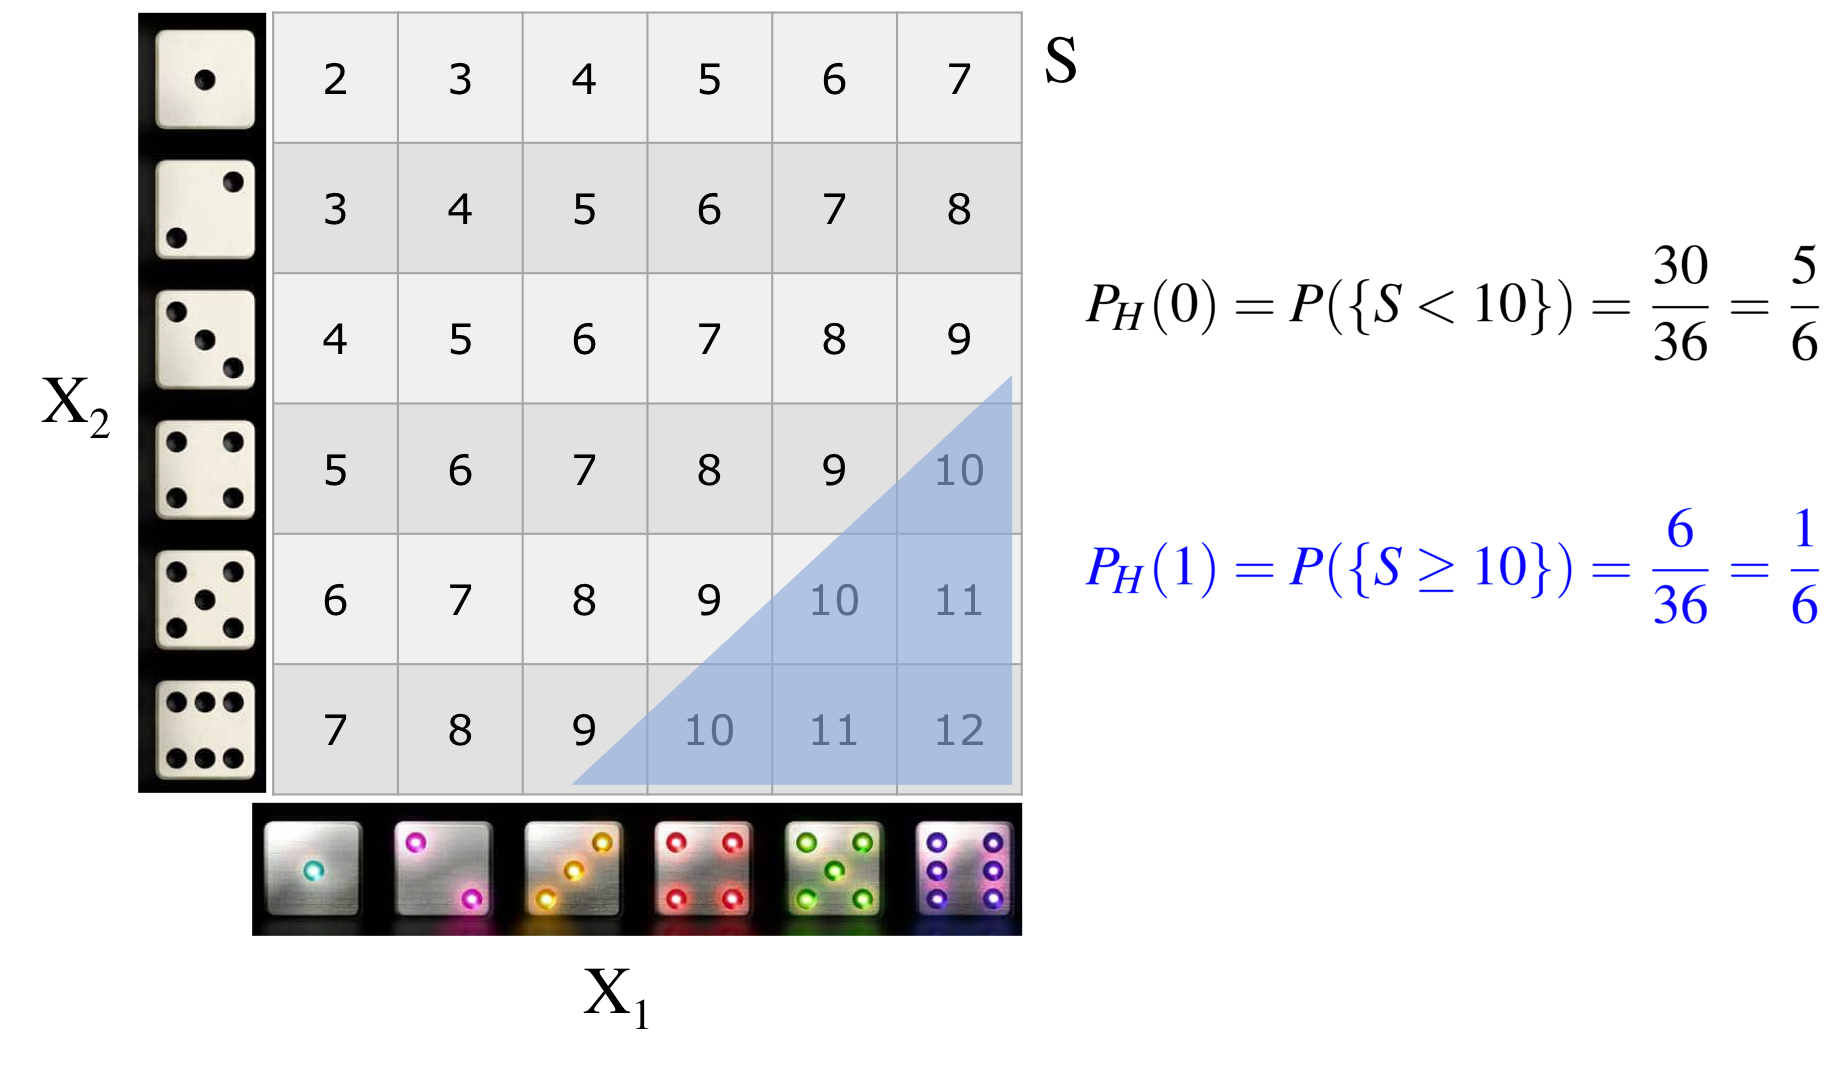
\includegraphics[width=10cm]{Figures/Dice.png}
        \end{center}
        \caption{All combinations of of $X_1$ and $X_2$ are equally probable, and therefore each of the $36$ results represented in the figure have a probability of $1/36$. Counting the number of occurrences of particular values of $S$ or $H$, the distribution of these variables can be calculated.\label{fig:dice}}
    \end{figure}
    
    Since we have to provide the criterion that minimizes the probability of error, we can then conclude that we should always decide in favor of hypothesis 0:
    $$d^\star = 0,$$
with a probability of error of  $1/6$.
    
    A final remark is in order. Note that the probability of error of each criterion is given by the {\em a priori} probability of the complementary hypothesis. This implies that, to minimize the probability of error, we have to decide in favor of the hypothesis with a larger {\em a priori} probability.

    \item[b)] In real applications, there are scenarios where not all the errors should be given the same importance. Here, we introduce the concept of {\em cost} to model the penalty that should be assigned to different kinds of errors.\footnote{In some cases rather than working with the minimization of a cost we might pursue the maximization of a profit. Both scenarios can be shown to be completely equivalent, but in this course we will always deal with cost functions.}
    
    Since different kinds of errors can be observed in different experiments, the cost can also be modeled with a random variable $C$. In this particular problem, $C$ can take four different values that we will denote as $c_{dh}$, for $d, h \in \{0,1\}$. That is, $c_{dh}$ is the cost of deciding $d$ when the true hypothesis was $h$. According to the wording, the costs are:
    \begin{equation*}
    c_{dh} = \left\{ \begin{array}{l}c_{00}=c_{11}= 0 \\ c_{01} = 1 \\ c_{10} = c\end{array}\right.    
    \end{equation*}
    
    Since $C$ is a function of $H$, it is also a random variable, for which its distribution could be obtained (from the probability distribution of $H$, $P_H(h)$). However, in this problem we only need to compute the expected cost of both detectors, that is,
    
    \begin{itemize}
        \item For the detector $d=0$:
        $$\widebar C = \mathbb{E}\{c_{dh}\} = \mathbb{E}\{c_{0h}\} = \sum_{h=0}^1 c_{0h} P_H(h) = c_{00}P_H(0) + c_{01}P_H(1) = \frac{1}{6}.$$
        \item For the detector $d=1$:
        $$\widebar C = \mathbb{E}\{c_{dh}\} = \mathbb{E}\{c_{1h}\} = \sum_{h=0}^1 c_{1h} P_H(h) = c_{10}P_H(0) + c_{11}P_H(1) = \frac{5 c}{6}.$$
    \end{itemize}

    \item[c)] To minimize the expected cost, we have to compare the costs that we calculated in the previous subsection
    $$\widebar C (d=0) \dunodcero \widebar C (d=1),$$
    which results in
    $$c \dceroduno \frac{1}{5}.$$
    
    Let us check, using our intuition, that this result makes sense. To start with, note that when the penalty given to wrongly deciding $d=1$ is unitary ($c_{10}=c=1$), both kinds of errors are identical. In such case, it can be seen that minimizing the expected cost is the same as minimizing the probability of error, and we should decide $d=0$ as in part a) of this problem. However, if $c_{10}$ is sufficiently small, deciding $d=1$ has a very small cost, so it can pay off to decide $d=1$ even though the number of errors is larger, as it will certainly be the case since hypothesis $H=0$ appears 5 times more often than hypothesis $H=1$. Hence, the expression above implies that if $c < 1/5$ then detector $d=1$ yields a smaller expected cost.
\end{itemize}
\end{solution}


\subsection{Example 2: Binary decision with observations}
\label{subsec:example2}

\begin{problem}
Consider now the scenario described in the previous example, with the difference that, before deciding in favor of one of the hypotheses, we are allowed to see the result of the first die, $X_1$. In this case, we will therefore be able to take a more informed decision since knowing such value carries information about the value of $S$.
\begin{itemize}
    \item [a)] Calculate the probability of error incurred by each possible decision ($d=0$ and $d=1$) for each value of $X_1$.
    \item [b)] Design the detector that minimizes the probability of error, and compute the probability of error of such detector.
    \item[c)] Obtain the test statistic that minimizes the cost described in the previous example, for the particular case $c=1/4$.
\end{itemize}
\end{problem}

\begin{solution}
The main difference of the scenario described in this problem with respect to that of the previous example is that, in this case, the detector can be a function of $X_1$. As a result, the decision may change from experiment to experiment, depending on the value of  $X_1$.

Precisely, when designing a detector our goal is to assign each possible value of the observations to a particular decision. In other words, if the same input is observed twice, the output must be the same in both cases, since the mapping from the observations to the decisions is assumed to be deterministic. We will say more on this later on, but for now, we focus on providing answers to the considered problem.

\begin{itemize}
    \item [a)] We will follow along the same lines of the previous exercise to compute the probability of error for the two possible decisions. Notice, however, that in this case we will be conditioning these probabilities on the value of $X_1$.
    \begin{itemize}
        \item For $x_1 \in \{1,2,3\}$, hypothesis $H=1$ can never hold. Therefore, in this case it seems obvious that deciding $d=0$ would guarantee a zero probability of error. More formally:
        $$\text{If } x_1 \in \{1,2,3\} \rightarrow \left\{\begin{array}{l} d=0 \rightarrow P_e = P(d\neq H|x_1\in \{1,2,3\}) = P_{H|X_1}(1|x_1\in \{1,2,3\}) = 0 \\ d=1 \rightarrow P_e = P(d\neq H|x_1\in \{1,2,3\}) = P_{H|X_1}(0|x_1\in \{1,2,3\}) = 1\end{array}\right.$$
        \item For $x_1 = 4$, there is only one possibility out of 6 that hypothesis $H=1$ is correct (for $x_2=6$). This allows us to easily compute the error of both criteria. Repeating this  for the remaining values of $X_1$, we obtain the following probabilities of error conditioned on $X_1$.
        $$\text{If } x_1 =4 \rightarrow \left\{\begin{array}{l} d=0 \rightarrow P_e = P(d\neq H|x_1=4) = P_{H|X_1}(1|x_1=4) = \frac{1}{6} \\ d=1 \rightarrow P_e = P(d\neq H|x_1=4) = P_{H|X_1}(0|x_1=4) = \frac{5}{6}\end{array}\right.$$
        $$\text{If } x_1 =5 \rightarrow \left\{\begin{array}{l} d=0 \rightarrow P_e = P(d\neq H|x_1=5) = P_{H|X_1}(1|x_1=5) = \frac{2}{6} = \frac{1}{3}\\ d=1 \rightarrow P_e = P(d\neq H|x_1=5) = P_{H|X_1}(0|x_1=5) = \frac{4}{6} = \frac{2}{3}\end{array}\right.$$
        $$\text{If } x_1 =6 \rightarrow \left\{\begin{array}{l} d=0 \rightarrow P_e = P(d\neq H|x_1=6) = P_{H|X_1}(1|x_1=6) = \frac{3}{6} =\frac{1}{2} \\ d=1 \rightarrow P_e = P(d\neq H|x_1=6) = P_{H|X_1}(0|x_1=6) = \frac{3}{6} = \frac{1}{2}\end{array}\right.$$
    \end{itemize}
In this case, the probability of error associated to each decision is given by the probability of the complementary hypothesis. The difference is that now we have to use {\em a posteriori} probabilities of the hypotheses, given that the decision is taken using some information (the value of $X_1$), and this knowledge refines how likely we can expect the different hypotheses to be. Figure \ref{fig:posteriorprobs} depicts these probabilities. Note that to compute the probability conditioned on each value of $X_1$, we need to consider only the values of $S$ that are associated to the corresponding column.
    
    \begin{figure}
        \begin{center}
            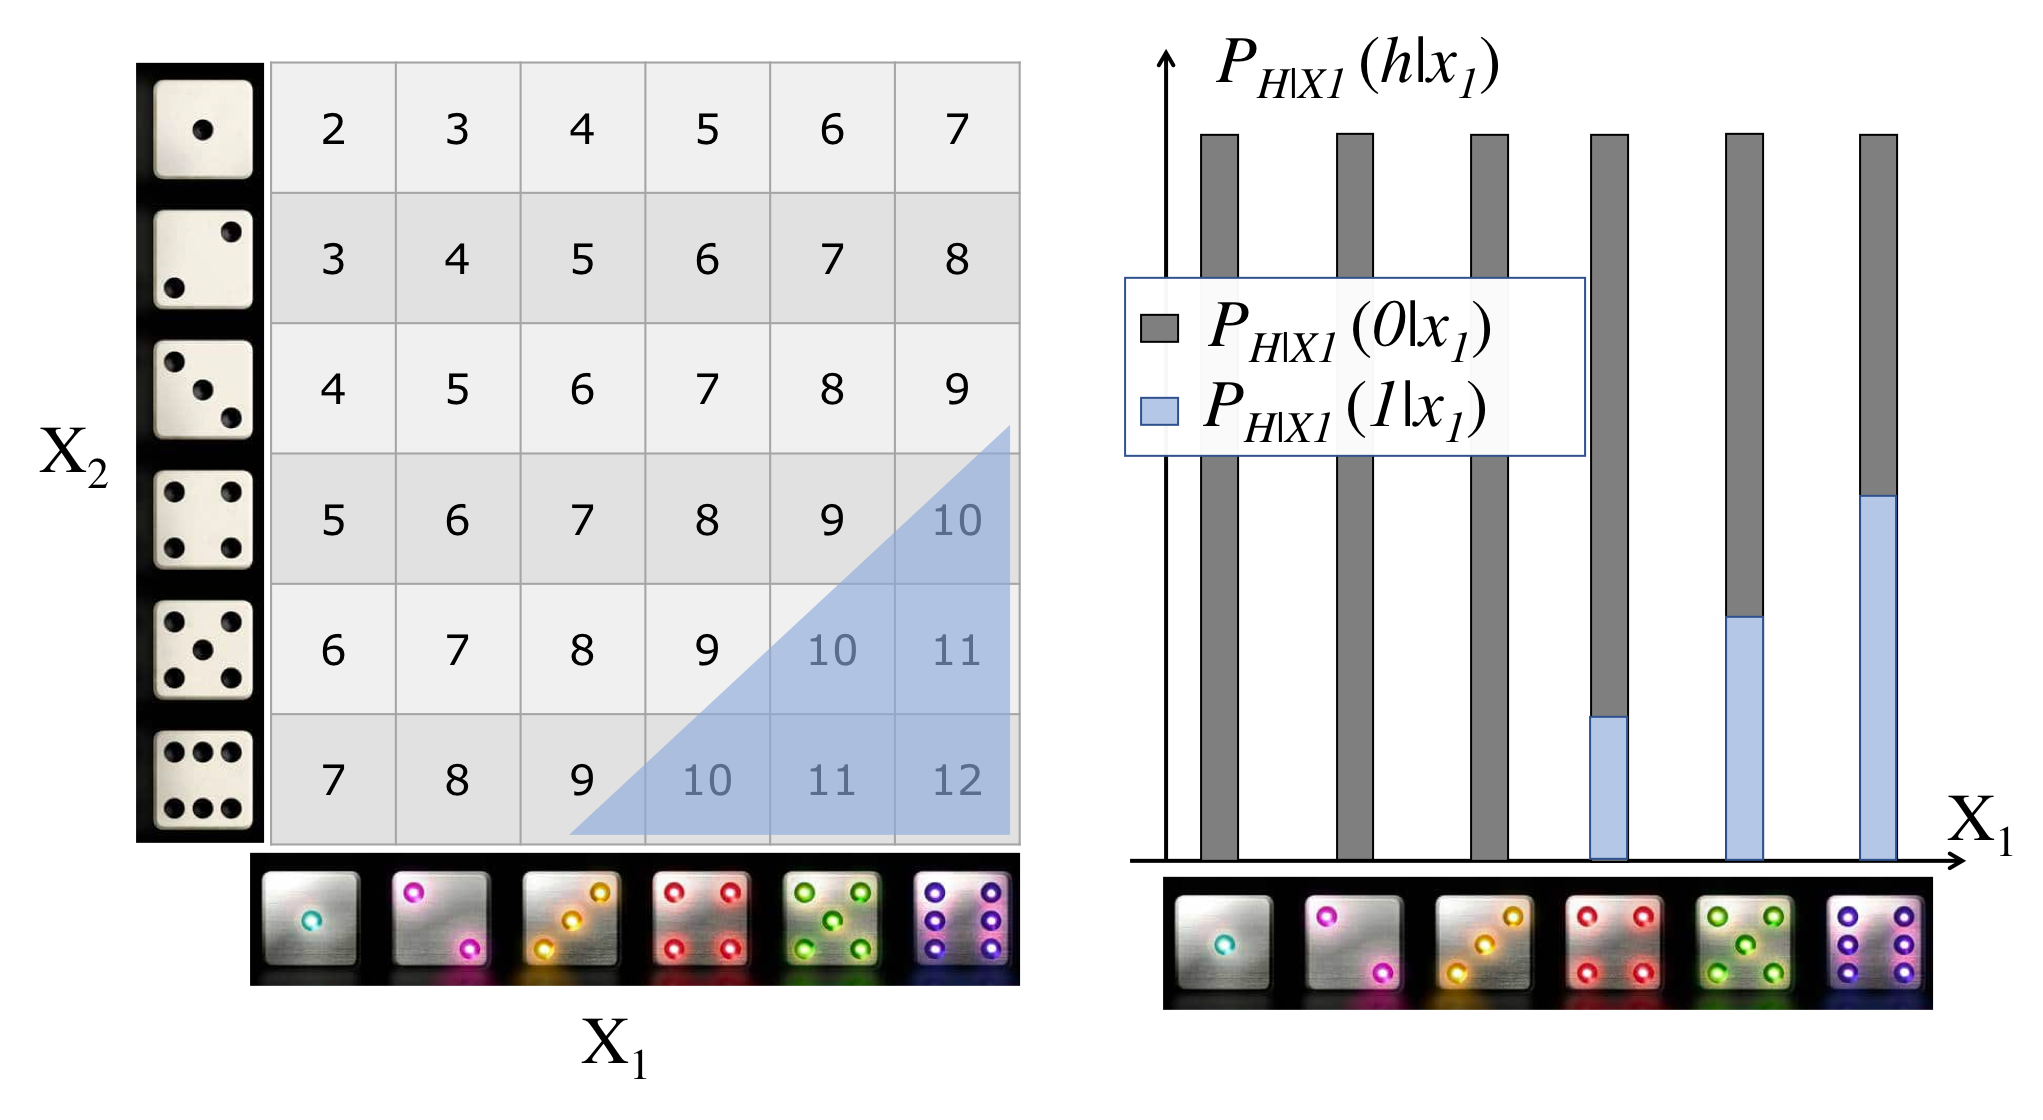
\includegraphics[width=10cm]{Figures/Dice_posterior.png}
        \end{center}
        \caption{To calculate posterior probabilities of the hypothesis, we need to count how many results in each column correspond to hypothesis 0 and how many correspond to hypothesis 1. Note that $P_{H|X_1}(0|x_1) + P_{H|X_1}(1|x_1) = 1$ for all values of $X_1$.\label{fig:posteriorprobs}}
    \end{figure}

    \item[b)] To minimize the probability of error of the detector, it suffices to minimize the conditional probability of error. In this case, since the decision becomes a function of $X_1$, $D = f(X_1)$, the detector becomes a random variable itself. Designing the detector consists in obtaining such function $f(\cdot)$. In this course, we only consider that $f(\cdot)$ is deterministic, i.e., if the same $x_1$ is observed twice the detector will produce the same output in both cases. This implies that we can alternatively interpret the goal of designing a detector as partitioning the observation space into as many regions as the number of hypotheses.
    
    Using the results from the previous section, it follows that, to minimize the error at every point, we need to select the hypothesis with the largest {\em a posteriori} probability, i.e., the test statistic that results in a minimum probability of error is:
    $$d(x_1) =\arg\max_i P_{H|X_1}(i|x_1).$$
    This expression gives the name to the detection criterion, is known as the {\em Maximum a Posteriori} (MAP) detector. Actually, maximizing the {\em a posteriori} probability is the criterion that minimizes the probability of error in general. 
    
    Since $P_{H|X_1}(0|x_1=6) = P_{H|X_1}(1|x_1=6)$, for $x_1 = 6$ deciding in favor of either hypotheses results in the same probability of error ($1/2$). For the remaining values, $d=0$ should be selected. Finally, using the law of total probability, the probability of error becomes
    \begin{align}P_e = P(D\neq H) & = \sum_{x_1=1}^6 P(D\neq H| x_1) P_{X_1}(x_1) \nonumber \\
    & = P(D\neq H| x_1=1) P_{X_1}(1) + P(D\neq H| x_1=2) P_{X_1}(2) \nonumber \\
    & \;\;\;\;\;\;+ P(D\neq H| x_1=3) P_{X_1}(3) + P(D\neq H| x_1=4) P_{X_1}(4) \nonumber \\
    & \;\;\;\;\;\;+ P(D\neq H| x_1=5) P_{X_1}(5) + P(D\neq H| x_1=6) P_{X_1}(6) \nonumber \\
    & = \frac{1}{6} \left[0 + 0 + 0 + \frac{1}{6} + \frac{1}{3} + \frac{1}{2}\right] = \frac{1}{6}.\nonumber
    \end{align}
    
    \item[c)] In this part of the problem we need to minimize the expected cost. Similarly to what we did for the probability of error, we will first compute the expected cost associated to every decision and observation $x_1$, and then at each point we will simply select the decision criterion that incurs in a minimum expected cost.
    
    $$\text{If } x_1 \in \{1,2,3\} \rightarrow \left\{\begin{array}{l} d=0 \rightarrow \mathbb{E}\{C_{0H}|x_1\in \{1,2,3\}\} = 0 \\ d=1 \rightarrow \mathbb{E}\{C_{1H}|x_1\in \{1,2,3\}\} = c_{10} P_{H|X_1}(0|x_1\in \{1,2,3\}) = c_{10} = \frac{1}{4}\end{array}\right.$$
    $$\text{If } x_1 =4 \rightarrow \left\{\begin{array}{l} d=0 \rightarrow \mathbb{E}\{C_{0H}|x_1=4)\} = c_{01} P_{H|X_1}(1|x_1=4) = \frac{1}{6} \\ d=1 \rightarrow \mathbb{E}\{C_{1H}|x_1=4)\} = c_{10} P_{H|X_1}(0|x_1=4) = \frac{5}{24}\end{array}\right.$$
    $$\text{If } x_1 =5 \rightarrow \left\{\begin{array}{l} d=0 \rightarrow \mathbb{E}\{C_{0H}|x_1=5)\} = c_{01} P_{H|X_1}(1|x_1=5) = \frac{2}{6} \\ d=1 \rightarrow \mathbb{E}\{C_{1H}|x_1=5)\} = c_{10} P_{H|X_1}(0|x_1=5) = \frac{1}{6}\end{array}\right.$$
    $$\text{If } x_1 =6 \rightarrow \left\{\begin{array}{l} d=0 \rightarrow \mathbb{E}\{C_{0H}|x_1=6)\} = c_{01} P_{H|X_1}(1|x_1=6) = \frac{1}{2} \\ d=1 \rightarrow \mathbb{E}\{C_{1H}|x_1=6)\} = c_{10} P_{H|X_1}(0|x_1=6) = \frac{1}{8}\end{array}\right.$$
    
    Then, the detector that minimizes the expected cost is
%    \begin{equation}
  %      
   % \end{equation}
   \begin{equation*}
   d^\star = \begin{cases}  0, & \text{if } X_1 \in \{1,2,3,4\}, \\ 1, & \text{if } X_1 \in \{5, 6\},
   \end{cases}
   \end{equation*}
    with the expected cost given by
    \begin{align*}
        \mathbb{E}\{C\} & = \sum_{x_1=1}^6 \mathbb{E}\{C | x_1\} P_{X_1}(x_1) \\ &= \frac{1}{6}[0+ 0 +0 + \frac{1}{6} + \frac{1}{6} + \frac{1}{8}] \\ &= \frac{11}{6\cdot 24},
    \end{align*}
    which follows from the law of total probability. One final comment is in order. Using a detector that exploits the value of an observation variable, we were able to reduce the expected cost with respect to the value obtained in the first example.
    
\end{itemize}

\end{solution}

So far, we have learned that the {\em a posteriori} probability of $H$ given the observations plays a key role in detection problems. In the first two examples, obtaining such probability was rather straightforward given the inherent mechanism for the generation of the hypotheses: observations take place first, and the hypothesis depends directly on these observations. Now, we will consider the case in which the generation of the hypothesis occurs first, and then observations are drawn according to their probability distribution given the hypothesis. This scenario is frequently encountered in many real problems. When this is the case, one can more easily get access to the {\em likelihoods} of each hypothesis, and the {\em a posteriori} probabilities need to be evaluated exploiting Bayes' Theorem.

\subsection{Example 3: Working the solution from the likelihoods}
\label{subsec:example3}

\begin{problem}
	Consider now a new game that involves two coins, one of them is fair whereas for the second one, the probability of heads doubles the probability of tails. In this game, a coin is first selected, and the goal is to guess which is the selected coin using as observations the result of flipping the coin $n$ times. Therefore, this problem can also be seen as a hypothesis testing problem, where one has to decide whether the selected coin was the fair one (hypothesis $H=0$) or the loaded one (hypothesis $H=1$).
	
	\begin{itemize}
		\item [a)] Without assuming any other information, design a detector for the aforementioned hypothesis test.
		\item [b)] Discuss how you would design a detector that minimizes the probability of error, and what additional information you would need for that.
	\end{itemize}
\end{problem}

\begin{solution}
	
	We denote by $\bf X$ the vector that  contains all the available observations to take the decision, i.e., the result of each coin flipping: ${\bf X} = (X^{(1)}, X^{(2)}, \ldots, X^{(n)})^\top$. Each of these variables can be a head or a tail: $X^{(i)} \in \left\{\circ,\times \right\}$. We will denote by $n_\circ$ and $n_\times$ the number of observed heads and tails, respectively. Obviously, we have $n = n_\circ + n_\times$.
	
	\begin{itemize}
		\item [a)] The only statistical information available in this section is the probability of observing a head or a tail for both hypotheses:
		\begin{align*}
		P_{X^{(i)}|H}(\circ | 0) &= \frac{1}{2}, & P_{X^{(i)}|H}(\times | 0) &= \frac{1}{2},
		\end{align*}
		and
		\begin{align*}
		P_{X^{(i)}|H}(\circ | 1) &= \frac{2}{3}, & P_{X^{(i)}|H}(\times | 1) &= \frac{1}{3}.
		\end{align*}
		Now, since there are available $n$ observations, we can also compute the joint probability of the observation vector $\bf X$:
		\begin{align*}
		P_{{\bf X}|H}({\bf x}|0) &= \left( \frac{1}{2}\right)^{n}, & P_{{\bf X}|H}({\bf x}|1) &= \left( \frac{2}{3}\right)^{n_\circ} \left( \frac{1}{3}\right)^{n_\times}.
		\end{align*}		
		These two expressions above are the joint probabilities of all observed variables given the hypothesis, and are usually referred to as the likelihoods of hypothesis $0$ and $1$. Essentially, the likelihoods express how well the observed data can be explained by each of the hypotheses.
		
		When the only available information is the likelihoods, a reasonable approach to follow is deciding in favor of the hypothesis that maximizes the likelihood. For this example, the so-called {\em maximum likelihood} (ML) detector is given by
		$$P_{{\bf X}|H}({\bf x}|0)\dceroduno P_{{\bf X}|H}({\bf x}|1) \Rightarrow \left( \frac{1}{2}\right)^{n} \dceroduno \left( \frac{2}{3}\right)^{n_\circ} \left( \frac{1}{3}\right)^{n_\times}.$$
		A convenient way to simplify this expression consists in taking logarithms on both sides of the inequality. Note that, in order to take logarithms, we need to make sure that the arguments thereof are strictly positive, which holds for both sides of the equation above. Then, taking logarithms and simplifying the resulting expression yields
		$$(n_\circ + n_\times) \log\frac{1}{2} \dceroduno n_\circ \log\frac{2}{3} + n_\times \log\frac{1}{3},$$
		or, equivalently,
		$$\frac{n_\times}{n_\circ} \dceroduno \frac{\log\frac{2}{3} - \log\frac{1}{2}}{\log\frac{1}{2} - \log\frac{1}{3}}.$$
		This equation translates into a partition of the observation space. In fact, we see that the detector does not depend on the value of particular observations, but just on the total number of heads and tails (i.e., the order in which the coin flippings are observed does not matter). Moreover, it also implies that a larger number of observed heads favors the decision $D=1$, which aligns with the fact that the probability of heads is larger than the probability of tails when $H=1$.
		
		\item[b)] Now, we need to study the minimization of the probability of error, defined as
		$$P_e = P(D\neq H) = \sum_{\bf x} P(d\neq H | {\bf X}={\bf x}) P_{\bf X}({\bf x}).$$
		In order to grasp the meaning of $P_e$, we need to emphasize that for any particular detector, there is a deterministic relation between $D$ and ${\bf X}$. Since the probability of error for a given observation vector is $P(d\neq H | {\bf X}={\bf x})$, the expectation of this value needs to be taken with respect to ${\bf X}$ to obtain the probability of error. The minimization of $P_e$ is equivalent to the minimization of each element in the above summation. That is, for each possible observation vector ${\bf x}$ we need to take the decision that minimizes the probability of error for that particular value of ${\bf x}$. Since there are only two hypothesis, the probability of incurring in an error if we decide in favor of one of the hypothesis is the probability of the non-selected hypothesis, i.e.,
		$$\text{If we decide } d=0 \qquad \rightarrow \qquad  P(H \neq 0 | {\bf X}={\bf x}) = P_{H|{\bf X}}(1|{\bf x}),$$
		$$\text{If we decide } d=1 \qquad \rightarrow \qquad  P(H\neq 1 | {\bf X}={\bf x}) = P_{H|{\bf X}}(0|{\bf x}).$$
		Therefore, in order to minimize the probability of error at each ${\bf x}$, and therefore to minimize the overall probability of error, we need to follow the criterion:
		$$P_{H|{\bf X}}(1|{\bf x}) \dunodcero P_{H|{\bf X}}(0|{\bf x}),$$
		which is, as described above, the {\em Maximum a posteriori} (MAP) detector. In other words, maximizing the likelihood does not necessarily minimize the probability of error, which is actually minimized by maximizing the {\em a posteriori} probabilities of each hypotheses. This makes sense, since the likelihood just measures how well the observations fit with a given hypothesis, but ignores the {\em a priori} probability of the hypotheses. Then, we can  decide in favor of a hypotheses with smaller likelihood if its {\em a priori} probability is sufficiently larger than the probability of the other hypothesis. This can be explicitly quantified by means of Bayes' Theorem, which states that
		$$P_{H|{\bf X}}(h|{\bf x}) = \frac{P_{{\bf X}|H}({\bf x}|h) P_{H}(h)}{P_{\bf X}({\bf x})}.$$
		Bayes' Theorem shows that the maximization of  the {\em a posteriori} probability of each hypothesis (and therefore to minimize the probability of error) requires taking into account both the likelihoods and the {\em a priori} probabilities of the hypotheses.
		
		In summary, in order to design a detector (or classifier) that minimizes the probability of error, we would need to know the {\em a priori} probability of each hypothesis. Moreover, if the goal were to minimize a cost function, we would still need to rely on {\em a posteriori} probabilities.
		
	\end{itemize}
	
\end{solution}

In the previous examples, we have introduced a number of important concepts in detection problems: hypotheses, {\em a priori} and {\em a posteriori} probability, likelihood, probability of error, and (expected) cost. We have also learned that, for the design of detectors when there are available observations, the distribution that provides {\bf  the most valuable information is the {\em a posteriori} distribution of the hypotheses given such observations}. If this distribution is available, we can compute the performance of {\bf any} detector in terms of its probability of error or expected cost (performance analysis problems). Based on these performance metrics, we can also design detectors that minimize each criterion (design problem). 

%\begin{problem}
%    Transmission of a binary symbol over a Gaussian channel (TBD).
% \end{problem}
\section{Introduction to Detection Theory}
\label{sec:SDT}

Once we have presented some of the main concepts involved in detection problems through a series of examples, we are ready to formalize the theory for the case of two or more hypotheses.

\subsection{Hypotheses-based problems}
\label{subsec:hypotheses_problems}

As we have already explained, in this course, we will only cover a particular class of detection or classification problems to which we will refer as {\em hypotheses-based problems}. The goal is to infer the correct hypothesis, which cannot be directly observed, from a set of measurements or observations.  Thus, we consider a scenario with $M$ hypotheses, and denote the random variable that identifies the hypothesis as $H$. This is depicted in Fig. \ref{fig:clas_overview}, where $H \in \{0, 1, \ldots, M-1\}$. We also assume that we have access to an observation vector $\bf x$, which can be considered as the realization of a random variable $\bf X$ lying in observation space $\cal X$. We assume also that there is a certain statistical relationship between $H$ and $\bf X$. Otherwise, i.e., if $H$ and $\bf X$ were independent, it would make no sense to use $\bf x$ to make an informed inference about the value of $H$.

    \begin{figure}
        \begin{center}
            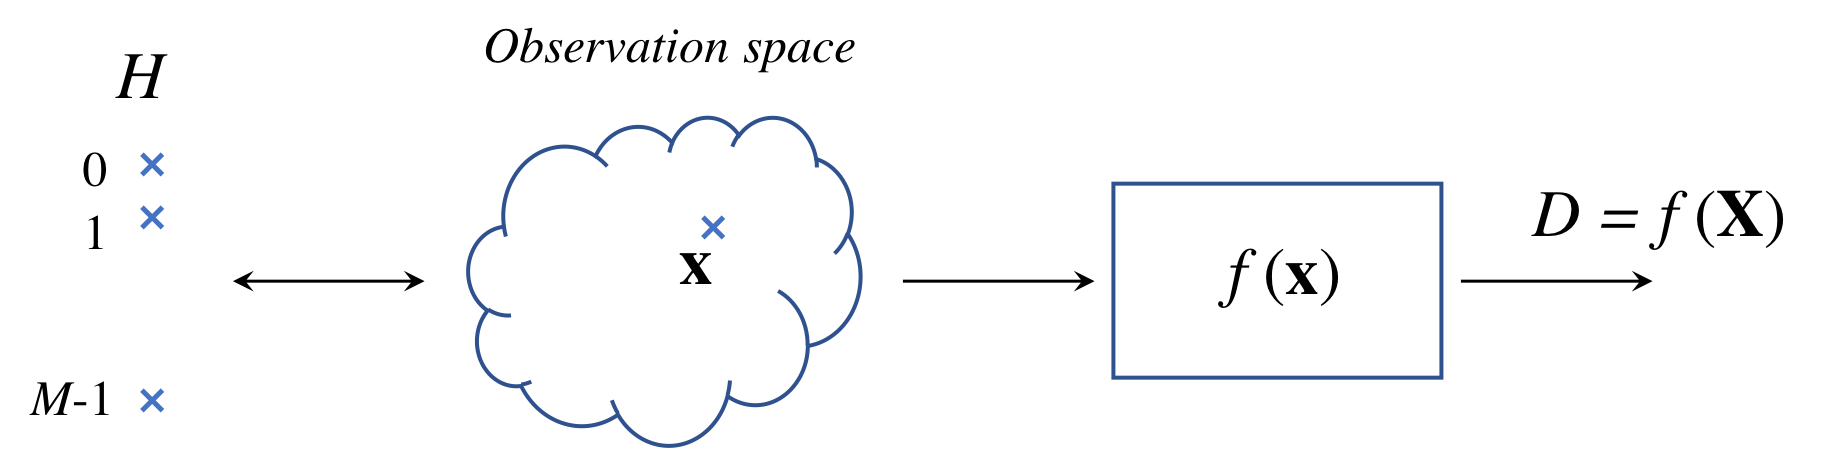
\includegraphics[width=10cm]{Figures//classification_overview.png}
        \end{center}
        \caption{Diagram block of hypothesis testing problems.\label{fig:clas_overview}}
    \end{figure}

In this context, a detector or classifier is a function of $\bf x$ that outputs a value $d$ in the range $\{0, 1, \ldots M-1\}$, i.e., a guess on the value of the hypothesis that is unknown beforehand. We should make a few considerations about the functions $f({\bf x})$ that we admit as valid detectors in this course:

\begin{itemize}
    \item We consider that $d = f({\bf x})$ is a deterministic function. This implies that if the same vector is presented several times, the function will output the same value each time. Note that, even though $f(\cdot)$ is deterministic, its output can be modeled as a random variable since the input is the random vector $\bf X$.
    \item The function is surjective, that is, every input ${\bf x}$ generates one and only one output. Hence, the function divides the observation space into $M$ non-overlapping regions, ${\cal X}_d$, $d = 0, 1, \ldots M-1$, i.e., one region per hypotheses. Moreover, the boundaries between regions are known as decision boundaries.
\end{itemize}

\begin{example}
The detector $f(x) = u(x^2 -1)$, where $u(\cdot)$ is the step function, is defined for any $x$ on the real line, and is characterized by the following decision regions:
\begin{align}{\cal X}_0 & = \left\{ x \in \Re | x^2-1 < 0\right\} = (-1,1) \nonumber\\
{\cal X}_1 & = \left\{ x \in \Re | x^2-1 \geq 0\right\} = (-\infty,-1] \cup [1,\infty) \nonumber
\end{align}
where we have assumed $u(0)=1$. In this example, the regions are connected and non-empty.
\end{example}

\begin{example}
\label{ex:decisionregions}
The decisor $f({\bf x}) = \arg\min_i y_i({\bf x})$ defined over ${\cal X} = [0,1]^2$, with
\begin{align}
y_0({\bf x}) & = \|{\bf x}\|^2 \nonumber \\
y_1({\bf x}) & = x_1 - x_0 +1 \nonumber \\
y_2({\bf x}) & = x_0 - x_1 + 1 \nonumber 
\end{align}
is characterized by the decision regions depicted in Fig. \ref{fig:decisionregions}.

    \begin{figure}
        \begin{center}
            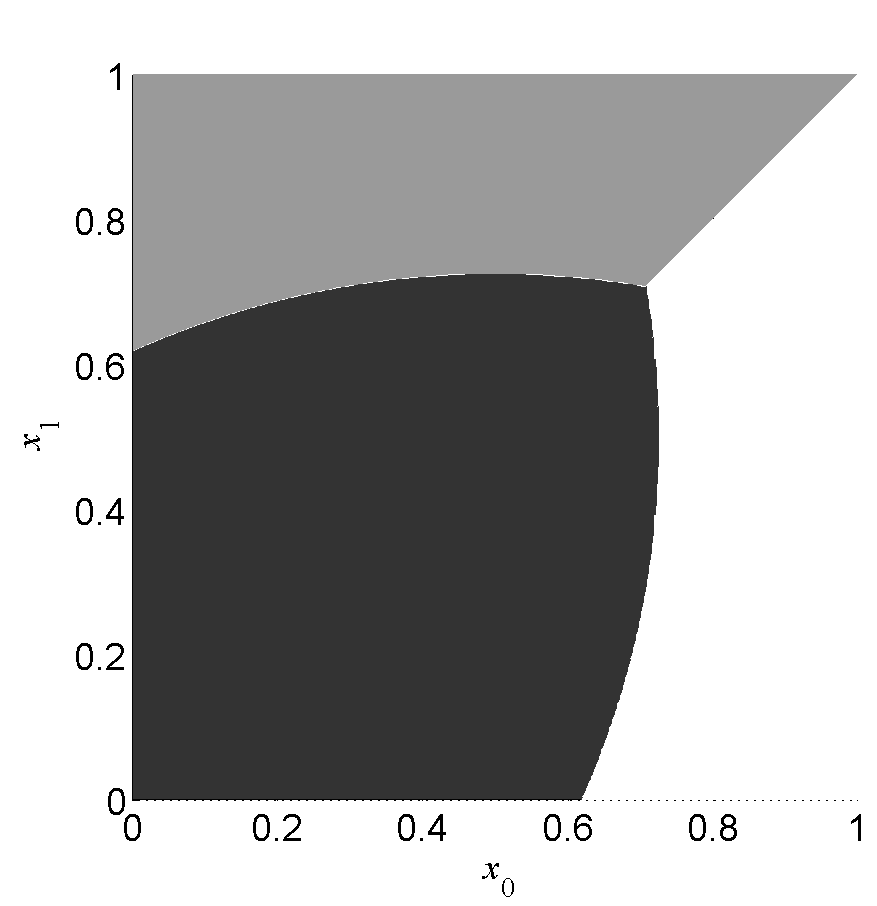
\includegraphics[width=6cm]{Figures//DecRegEx.pdf}
        \end{center}
        \caption{Decision regions for the detector given in Example \ref{ex:decisionregions}: ${\cal X}_0$ (black), ${\cal X}_1$ (grey), and ${\cal X}_2$ (white).\label{fig:decisionregions}}
    \end{figure}
    
\end{example}

\subsection{Statistical information involved in detection problems}
\label{subsec:statistical_info}

We review now the main distributions that will be employed in detection problems:
\begin{itemize}
    \item {\em A priori} probability distribution of the hypotheses: This is a discrete distribution that quantifies the probability of each hypothesis independently of the observations. If we did not have access to any observations, our design would have to rely entirely on these probabilities, as it was the case in Section \ref{subsec:example1},
    $$P_H(h), \qquad \text{ for } \quad h = 0, 1, \ldots,\;M-1.$$
    
    \item Likelihoods of the hypotheses: This represents the probability of the observations given the hypothesis. Note that, even though we refer to these distribution as the likelihoods of the hypotheses, what we actually have is a collection of distributions over the random variable $X$ (unidimensional case) or ${\bf X}$ (multidimensional case), one for each hypothesis,
    $$p_{{\bf X}|H}({\bf x}|h) \qquad \text{ for } \quad {\bf x} \in {\cal X} \text{ and } h = 0, 1, \ldots,\; M-1.$$
    where we have assumed a multidimensional case with continuous observations. Note that random variable $\bf X$ may lie in different regions depending on the hypothesis.
    
    \item {\em A posteriori} distribution of the hypotheses: This distribution provides information about the probabilities of the hypothesis, but conditioning them on each possible value of the observation vector
    $$P_{H|{\bf X}}(h|{\bf x}), \qquad \text{ for } \quad h = 0, 1, \ldots,\; M-1.$$
    Since designing a detector consists in deciding what should be the decision for each value of the observation vector, and this distribution expresses directly what are the probabilities of the hypothesis conditioned on every $\bf x$, {\em a posteriori} probabilities play a fundamental role for the statistical design of detectors. 
    
\end{itemize}

{\em A priori} and {\em a posteriori} probabilities are related by Bayes' Theorem, which states
    $$P_{H|{\bf X}}(h|{\bf x}) = \frac{p_{{\bf  X} | H}({\bf x}|h) P_H(h)}{p_{\bf X}({\bf x})}.$$
Bayes' Theorem shows how observing $\bf x$ modifies the information about the probabilities of the different hypotheses. Without them, we could only use $P_H(h)$ to make decisions. However, once the observation vector comes into play, a more accurate estimation of these probabilities can be achieved via $P_{H|{\bf X}}(h|{\bf x})$, and these probabilities can be used to obtain a more informed decision. Note also that if we know both the {\em a priori} probabilities of the hypothesis and their likelihoods, the joint distribution of $\bf X$ and $H$ can be calculated. This joint distribution is the most complete characterization of the random variables, and from it any other probability function can be calculated as well.

In the following, we consider two different kinds of problems involving $M$-ary hypothesis testing problems:
\begin{itemize}
	\item Analysis of detectors: Here, the detector is given, and the objective is to analyze its performance with respect to certain performance metrics.
	\item Detector design: The goal is to build a function $f(\bf x)$ to optimize a performance metric.
\end{itemize}

\section{Analysis of the detection performance}
\label{subsec:analysis}

The first problem that we consider is the evaluation of the performance of a given detector. In this section, we review different metrics that can be used to assess performance. In all cases, we consider first the multiple hypothesis test scenario, and afterwards we specialize it to the binary case.

\subsection{Probability of error}

The probability of error is the probability of a wrong decision, i.e., the output of the statistic is not equal to the actual hypothesis. Under a frequentist approach, this probability can be interpreted as the average number of experiments in which an incorrect decision is taken, when the number of experiments tends to infinity. However, since we are assuming that the statistical characterization of the problem is available through the different probability distributions that we just reviewed, the probability of error can be calculated in closed-form as:
\begin{align}
    P_e = P(D\neq H) & = 1 - P(D=H) \nonumber \\
    & = 1 - \sum_{h=0}^{M-1} P(D=h, H=h) \nonumber \\
    & = 1 - \sum_{h=0}^{M-1} P(D=h| H=h) P_H(h) \nonumber \\
    & = 1 - \sum_{h=0}^{M-1} P_H(h) \int_{{\cal X}_h} p_{{\bf X}|H}({\bf x}|h) d{\bf x}\nonumber
\end{align}
where we have exploited that the probability of error is one minus the probability of correct decision. This is , in most cases, more convenient since the number of combinations where $D$ and $H$ are equal is (much) smaller than the number of combinations where they differ. Moreover, the last line of the previous expression follows from
$$P(D=h| H=h) = P({\bf x}\in {\cal X}_d| H=h) = \int_{{\cal X}_h} p_{{\bf X}|H}({\bf x}|h) d{\bf x},$$
which states that, conditioned on $H=h$, the probability of $D=h$ is precisely the integral of the likelihood of that hypothesis in the region where the given detector decides in favor of hypothesis $h$, i.e., the region ${\cal X}_h$.

Finally, note that it is also possible to compute the probability of error for a particular observation vector ${\bf x}$. If ${\bf x}$ belongs to ${\cal X}_d$, the associated probability of error would be
\begin{equation}
    P(H\neq d|{\bf x}) = 1 - P( H = d|{\bf x}) = 1 - P_{H|{\bf X}}(d|{\bf x}) = \sum_{\substack{l = 0 \\ l \neq d}}^{M-1} P_{H|{\bf X}}(l|{\bf x})
    \label{eq:Pe_x}
\end{equation}
In other words, the probability of error at a particular ${\bf x} \in {\cal X}_d$ is the sum of the {\em a posteriori} probabilities of hypothesis different from $d$ conditioned on this particular observation. For instance, imagine that in a three-hypothesis testing problem for a given ${\bf x}_o$ a detector selects hypothesis $0$. Then, the probability of error for  ${\bf x}_o$ is the sum of the probabilities of hypothesis $1$ and $2$ conditioned on ${\bf X} = {\bf x}_o$, i.e., the sum of {\em a posteriori} probabilities $P_{H|{\bf X}}(1|{\bf x}_o)$ and $P_{H|{\bf X}}(2|{\bf x}_o)$.

\subsubsection{Binary case: $P_e$, $P_\text{FA}$, $P_\text{M}$ and $P_\text{D}$}
For the binary case, contrary to the multiple hypotheses test, computing the probability of error  involves as many terms as the probability of a correct decision since
\begin{align}
    P_e & = P(D=0, H=1) + P(D=1, H=0) \nonumber \\
    & = P(D=0|H=1) P_H(1) + P(D=1|H=0) P_H(0) \nonumber
\end{align}
In the expression above we find two terms that are normally referred to as the {\em probability of false alarm} (also known as probability of Type I error or significance level) and the {\em probability of missing} (or probability of Type II error):
\begin{align}
    P_\text{FA} & = P(D=1|H=0) = \int_{{\cal X}_1} p_{{\bf X}|H}({\bf x}|0) d{\bf x} \nonumber \\
    P_\text{M} & = P(D=0|H=1) = \int_{{\cal X}_0} p_{{\bf X}|H}({\bf x}|1) d{\bf x} \nonumber
\end{align}
Similarly, the probability of detection (or power) is defined as
$$P_\text{D} = P(D=1|H=1) = 1 - P_\text{M}$$
Using these definitions, the probability of error can now be expressed more compactly as
$$P_e = P_\text{M} P_H(1) + P_\text{FA} P_H(0)$$
Interestingly, for the computation of $P_\text{FA}$ and $P_\text{M}$, only likelihoods are required. However, in order to compute the overall probability of error, we also need to know the {\em a priori} probabilities of the hypothesis.

We also introduce here an important concept for the analysis of binary hypothesis tests: the receiver operating characteristic (ROC) curve. The ROC curve plots the probability of false alarm, $P_\text{FA}$, against the probability of detection, $P_\text{D}$. Figure \ref{fig:ROC} shows the ROC curves of two different detectors, Detector 1 and Detector 2. As can be seen in this figure, the performance of Detector 2 is clearly better than that of Detector 1, since for each $P_\text{FA}$, the $P_\text{D}$ of Detector 2 is equal or larger than that of Detector 1. Moreover, both detectors perform better than a random decision whose ROC curve is also shown in the figure. One final comment is in order. For almost all detectors it is not possible to increase the probability of detection without increasing the probability of false alarm.

\begin{figure}
        \begin{center}
			\includestandalone{Figures/ROC}
	\end{center}
	\caption{ROC curves for two different detectors.\label{fig:ROC}}
\end{figure}

\subsection{Average (or mean) cost}

Using the probability of error as the unique measure of the detector's performance is not a good idea, because there are many practical scenarios where not all errors are equally critical. Imagine, for instance, a detector that discriminates whether there are or not suspicious tumor masses in a medical image. Such detector is used as a pre-diagnosis system, so that patients that can have a tumor are then explored with more accurate (but also invasive) techniques. In this case, there is a clear asymmetry between both kinds of errors: The incorrect decision that tumor masses are present would result in an unnecessary biopsy and inconvenience for the patient,but the opposite error could delay the diagnosis until a time when the process is irreversible.

To assign a penalty to different kinds of errors, we can define a cost function $$c_{DH}, \qquad D,H = 0, \ldots, M-1.$$ Such function will take as many values as combinations of decisions and hypotheses, in such a way that each particular value $c_{dh}$ is the cost of deciding $D=d$ when hypothesis $H=h$ is the true one. As already pointed out, we assume deterministic costs in this course, in the sense that the cost for each particular $d$ and $h$ is fixed. However, since the cost is a function of the random variables $D$ and $H$, it is a random variable as well, and its expected value can be computed as
$$\mathbb{E}\left\{ c_{DH}\right\} = \sum_{h=0}^{M-1} \sum_{d=0}^{M-1} c_{dh} P(D=d, H=h).$$

In order to compute the expected cost in terms of the probability distributions of ${\bf X}$ and $H$, we can use the relationship between $D$ and ${\bf X}$, which yields
\begin{align}
\mathbb{E}\left\{ c_{DH}\right\} & = \sum_{h=0}^{M-1} \sum_{d=0}^{M-1} c_{dh} P({\bf x}\in {\cal X}_d, H=h) \nonumber \\
& = \sum_{h=0}^{M-1} P_H(h) \sum_{d=0}^{M-1} c_{dh} P({\bf x}\in {\cal X}_d| H=h) \nonumber \\
& = \sum_{h=0}^{M-1} P_H(h) \sum_{d=0}^{M-1} c_{dh} \int_{{\bf x}\in {\cal X}_d} p_{{\bf X}|H}({\bf x}|h) d{\bf x}.\nonumber
\end{align}
Finally, we can also compute the expected cost conditioned on a given value of ${\bf x}$. Taking into account that, for a given ${\bf x}$ and a given detector, the decision value is fixed, it is only required to take expectations with respect to such hypothesis. Consider, for instance, the computation of the mean cost for some value ${\bf x}$ belonging to ${\cal X}_d$. Thus, the expected cost is obtained as
\begin{equation}
    \mathbb{E}\left\{ c_{dH}\right|{\bf x}\} = \sum_{h=0}^{M-1} c_{dh} P_{H|X}(h|{\bf x}).
\label{eq:cost_x}
\end{equation}

\subsubsection{Binary case: Mean cost}

For the binary case, a simpler expression can be obtained in terms of $P_\text{FA}$, $P_\text{M},$ and $P_\text{D}$ as follows
\begin{align}
    \mathbb{E}\left\{ c_{DH}\right\} & = c_{00} P(D=0, H=0) + c_{01} P(D=0,H=1) \nonumber \\
    & \;\;\;\;\;\; + c_{10} P(D=1, H=0) + c_{11} P(D=1,H=1) \nonumber \\
    & = c_{00} P(D=0|H=0) P_H(0) + c_{01} P_\text{M} P_H(1) \nonumber \\
    & \;\;\;\;\;\; + c_{10} P_\text{FA}P_H(0) + c_{11} P_\text{D} P_H(1) .\nonumber
\end{align}

\section{Detector design}
\label{subsec:design}

Once we have studied different ways of analyzing the performance of a given detector, we turn our attention to the problem of designing detectors that maximize one of these performance metrics.

\subsection{Maximum likelihood and maximum \emph{a posteriori} detectors}

A first possibility would be to rely directly on the maximization of the available probability density functions:

\begin{itemize}
    \item The detector that maximizes the likelihood is known as the {\em maximum likelihood} (ML) detector:
    $$d_{ML} = \arg\max_h p_{{\bf X}|H}({\bf x}|h).$$
    \item The detector that selects the hypothesis with maximum {\em a posteriori} probability is known as the  maximum {\em a posteriori} (MAP) detector:
    $$d_{MAP} = \arg\max_h P_{H|{\bf X}}(h|{\bf x}).$$
\end{itemize}

These detectors proceed as follows. Designing a detector is equivalent to specifying a unique decision for each possible value of the observation vector ${\bf x}$. Then, the ML and MAP strategies are based on evaluating either the likelihoods or the {\em a posteriori} probabilities for each ${\bf x}$ in the observation space, and select, for each ${\bf x}$, the hypothesis that maximizes $p_{{\bf X}|H}({\bf x}|h)$ (ML) or $P_{H|{\bf X}}(h|{\bf x})$ (MAP).

Finally, there are two properties that are worth considering with respect to these detectors:
\begin{enumerate}
    \item When the {\em a priori} probabilities of the hypothesis are the same, i.e., $P_H(h) = 1/M$, the ML and MAP detectors are identical. This can be shown from the Bayes' Theorem, since in this case
    $$d_{MAP} = \arg\max_h P_{H|{\bf X}}(h|{\bf x}) = \arg\max_h \frac{p_{{\bf X}|H}({\bf x}|h) P_H(h)}{p_{\bf X}(\bf x)} = \arg\max_h p_{{\bf X}|H}({\bf x}|h) = d_{ML}$$
    
    \item The MAP detector minimizes the probability of error. Note that according to \eqref{eq:Pe_x} the probability of error for a given $\bf x$ can be expressed as
    $$P(D\neq H|{\bf x}) = 1 - P_{ H|{\bf X}}(h|{\bf x})$$
    Since the MAP detector selects for every $\bf x$ the hypothesis that maximizes $P_{H|{\bf X}}(h|{\bf x})$, it therefore minimizes the probability of error for each vector of the observation space. Thus, as the probability of error is minimized for each point of the observation space, it is also minimized overall. That is,
    $$P(D\neq H) = \int_{\mathcal{X}} P(D\neq H|{\bf x}) p_{\bf X}(\bf x) d{\bf x},$$
    and we can check that the value of the integral (the probability of error) is minimized if, for each $\bf x$, the decisions minimize $P(D\neq H|{\bf x})$, i.e., the MAP detector.
    
\end{enumerate}

\subsubsection{Binary case: ML and MAP detectors}

The expressions of the ML and MAP detectors become fairly simple for the binary case:
\begin{itemize}
    \item Maximum likelihood detector:
    $$p_{{\bf X}|H}({\bf x}|1) \dunodcero p_{{\bf X}|H}({\bf x}|0),$$
    which can be expressed as a {\em likelihood ratio test} (LRT)
    $$\displaystyle\frac{p_{{\bf X}|H}({\bf x}|1)}{p_{{\bf X}|H}({\bf x}|0)} \dunodcero 1,$$
    where we have taken into account that the likelihoods are non-negative. Sometimes, it will be more convenient to work with the {\em log-likelihood ratio test} (LLRT)
    \begin{equation}
    \label{eq:LLRT}
    \log \left[ \frac{p_{{\bf X}|H}({\bf x}|1)}{p_{{\bf X}|H}({\bf x}|0)} \right] = \log p_{{\bf X}|H}({\bf x}|1) - \log p_{{\bf X}|H}({\bf x}|0) \dunodcero 0,
    \end{equation}
    which can be done because the logarithm is a monotonically increasing function.
    \item Maximum \emph{a posteriori} detector:
    $$p_{H|{\bf X}}(1|{\bf x}) \dunodcero p_{H|{\bf X}}(0|{\bf x}),$$
    which can also be expressed as a LRT as
    $$\displaystyle\frac{p_{{\bf X}|H}({\bf x}|1)}{p_{{\bf X}|H}({\bf x}|0)} \dunodcero \displaystyle\frac{P_H(0)}{P_H(1)}.$$
\end{itemize}

As in the general case with $M$ hypothesis, the MAP detector minimizes the probability of error and the ML and MAP detectors are the same if $P_H(0)=P_H(1)=0.5$. Moreover, we can see that both detectors can be expressed as a LRT
    $$\displaystyle\frac{p_{{\bf X}|H}({\bf x}|1)}{p_{{\bf X}|H}({\bf x}|0)} \dunodcero \eta,$$
where $\eta$ is a threshold. When this threshold is $1$, the LRT is the ML detector and for $\eta = P_H(0)/P_H(1)$, the LRT becomes the MAP detector, that is, minimum $P_e$ detector. Hence, we get two different points in the ROC curve. Actually, sweeping the value of the threshold generates the complete ROC curves in Figure \ref{fig:ROC}.\footnote{This actually applies to all detectors that can be written as $\phi({\bf x}) \dunodcero \eta$. That is, comparing a function of the observations with a threshold achieves a given $(P_\text{FA},P_\text{D})$ point in the ROC curve. These detectors are known as threshold detectors.}

\subsubsection{Binary case: Neyman-Pearson detector}

The Neyman-Pearson (NP) detector is a well known detector for binary problems, which maximizes the probability of detection while it provides a bound on the probability of false alarm. Before proceeding with the derivation, let us recall the definitions of probability of false alarm and detection
\begin{align}
P_\text{FA} & = \int_{{\cal X}_1} p_{{\bf X}|H}({\bf x}|0) d{\bf x}, \nonumber \\
P_\text{D} & = \int_{{\cal X}_1} p_{{\bf X}|H}({\bf x}|1) d{\bf x}. \nonumber
\end{align}
Now, the NP detector can be derived as the solution to
\begin{equation*}
	\text{maximize } P_\text{D}, \quad \text{subject to } P_\text{FA} = \alpha,
\end{equation*}
which is an optimization problem with constraints. The solution this kind of problems is obtained from the Lagrangian, which is given by
\begin{align}
\mathcal{L}(\mathcal{X}_1,\eta) &= P_\text{D} - \eta (P_\text{FA} - \alpha) \nonumber \\
&= \int_{{\cal X}_1} p_{{\bf X}|H}({\bf x}|1) d{\bf x}  - \eta \left(\int_{{\cal X}_1} p_{{\bf X}|H}({\bf x}|0) d{\bf x} - \alpha \right) \nonumber \\
&= \int_{\mathcal{X}_1} \left( p_{{\bf X}|H}({\bf x}|1) - \eta p_{{\bf X}|H}({\bf x}|0)  \right) d  {\bf x} + \eta \alpha \nonumber
\end{align}
Note, that the optimization variable is the region where we decide $d=1$. Next, we need to maximize the Lagrangian, and therefore the $P_\text{D}$, which is achieved by maximizing the above integral. To do so, and taken into account that an integral may be seen as a sum, we need to design ${\cal X}_1$ such that the integrand is positive, i.e.
\begin{equation*}
	\mathcal{X}_1 = \{\mathbf{x} |p_{{\bf X}|H}({\bf x}|1) - \eta p_{{\bf X}|H}({\bf x}|0) \geq 0 \} \Rightarrow \frac{p_{{\bf X}|H}({\bf x}|1)}{p_{{\bf X}|H}({\bf x}|0)} \dunodcero \eta
\end{equation*}
and $\eta$ is selected to achieve the desired probability of false alarm.

\subsection{Minimum expected cost detector}

As we have already studied, sometimes it makes more sense to measure the performance of a detector in terms of the expected cost. Therefore, it is important to tackle the problem of designing a detector that is optimum with respect to the expected cost.

Remember that the expected cost of a detector deciding $d$ for an observation ${\bf x}$ is given by equation \eqref{eq:cost_x}, which we reproduce here for convenience:
\begin{equation}
    \mathbb{E}\left\{ c_{dH}\right|{\bf x}\} = \sum_{h=0}^{M-1} c_{dh} P_{H|X}(h|{\bf x}) \label{eq:mean_x_2}.
\end{equation}
Minimizing the expected cost over the whole observation space requires that decisions for each observation minimize the conditional expected cost. That is, for each ${\bf x}$ the above expression should be minimized, and the expression of the minimum mean cost detector can be stated as follows:
$$d^\star = \arg\min_{d} \sum_{h=0}^{M-1} c_{dh} P_{H|X}(h|{\bf x})$$
Hence, when designing the detector, we need to evaluate the cost of the different decisions for each observation vector, and select the decision for which the expected cost is minimized.

It is interesting to point out that when the cost function penalizes equally all kinds of errors, i.e.,
$$c_{dh} = \left\{\begin{array}{ll} 0, & \;\;\;\;d=h \\ c, & \;\;\;\;d\neq h\end{array}\right.$$
the detector with minimum expected cost becomes the MAP one. This is easily proved by replacing these costs into the expression for the minimum expected cost detector
\begin{align}
    d^\star & = \arg\min_{d} \sum_{h=0}^{M-1} c_{dh} P_{H|X}(h|{\bf x}) \nonumber \\
            & = \arg\min_{d} \ c \sum_{h\neq d} P_{H|X}(h|{\bf x}) \nonumber \\
            & = \arg\min_{d} \sum_{h\neq d} P_{H|X}(h|{\bf x}) \nonumber \\
            & = \arg\min_{d} 1 - P_{H|X}(d|{\bf x}) \nonumber \\
            & = \arg\max_{d} P_{H|X}(d|{\bf x}) \nonumber \\
            & = d_{MAP}.
\end{align}

\subsubsection{Binary case: Minimum expected cost detector}

In the binary case, we can also express the optimum detector with respect to a cost function as an LRT. Let us start by particularizing \eqref{eq:mean_x_2} for $d=0$ and $d=1$, and then follow the criterion of deciding in favor of the minimum cost, i.e.,
$$\mathbb{E}\left\{ c_{0H}\right|{\bf x}\} \dunodcero \mathbb{E}\left\{ c_{1H}\right|{\bf x}\}.$$
Now, using the definition of expectation, the criterion becomes
$$c_{00}P_{H|{\bf X}}(0|{\bf x}) + c_{01} P_{H|{\bf X}}(1|{\bf x})\dunodcero c_{10}P_{H|{\bf X}}(0|{\bf x}) + c_{11} P_{H|{\bf X}}(1|{\bf x}),$$
which after some algebra can be rewritten as
$$\displaystyle\frac{P_{H|{\bf X}}(1|{\bf x})}{P_{H|{\bf X}}(0|{\bf x})}\dunodcero \displaystyle\frac{c_{10}-c_{00}}{c_{01}-c_{11}}.$$
Finally, using Bayes' Theorem, we may rewrite the \emph{a posteriori} probabilities in terms of the likelihoods and the \emph{a priori} probabilities, which finally yields
$$\displaystyle\frac{P_{{\bf X}|H}({\bf x}|1)}{P_{{\bf X}|H}({\bf x}|0)}\dunodcero \displaystyle\frac{c_{10}-c_{00}}{c_{01}-c_{11}} \displaystyle\frac{P_H(0)}{P_H(1)},$$
and corresponds to yet another point of the ROC curve of the LRT.

\subsection{The Gaussian case}

In this section, we will derive the likelihood ratio test for Gaussian observation under several assumptions. Then, depending on the threshold, we would obtain the different detectors: NP, ML, MAP, and minimum cost.

Before proceeding, we introduce the multivariate real Gaussian probability density function (PDF), which is given by
\begin{equation}
P_{{\bf X}}({\bf x}) = \frac{1}{(2\pi)^{N/2} |{\bf V}|^{1/2}}
\exp\left(-\frac{1}{2}({\bf x}-{\bf m})^T {\bf V}^{-1}({\bf x}-{\bf m})\right)
\label{pXGauss}
\end{equation}
where ${\bf x}$ is an $N$-dimensional vector, ${\bf m}$ is the mean vector, and ${\bf V}$ is the cross-covariance matrix. Then, under hypothesis $h = 0$, the likelihood is
\begin{equation*}
P_{{\bf X}|H}({\bf x}|0) = \frac{1}{(2\pi)^{N/2} |{\bf V}_0|^{1/2}}
\exp\left(-\frac{1}{2}({\bf x}-{\bf m}_0)^T {\bf V}_0^{-1}({\bf x}-{\bf m}_0)\right),
\end{equation*}
whereas it is
\begin{equation*}
P_{{\bf X}|H}({\bf x}|1) = \frac{1}{(2\pi)^{N/2} |{\bf V}_1|^{1/2}}
\exp\left(-\frac{1}{2}({\bf x}-{\bf m}_1)^T {\bf V}_1^{-1}({\bf x}-{\bf m}_1)\right),
\end{equation*}
under hypothesis $h = 1$. For this hypothesis test, the LLRT in \eqref{eq:LLRT} becomes
\begin{multline*}
- \frac{1}{2}\log\left|{\bf V}_1 \right| 
- \frac{1}{2}({\bf x}-{\bf m}_1)^T {\bf V}_1^{-1}({\bf x}-{\bf m}_1) \\
+ \frac{1}{2}\log\left|{\bf V}_0 \right| 
+ \frac{1}{2}({\bf x}-{\bf m}_0)^T {\bf V}_0^{-1}({\bf x}-{\bf m}_0) 
\dunodcero \log(\eta) 
\end{multline*}
or, equivalently,
\begin{align}
({\bf x}-{\bf m}_0)^T {\bf V}_0^{-1}({\bf x}-{\bf m}_0) 
- ({\bf x}-{\bf m}_1)^T {\bf V}_1^{-1}({\bf x}-{\bf m}_1)
\dunodcero \mu
\label{eq:logLRTGauss}
\end{align}
where
\begin{equation*}
\mu = 2 \log(\eta) + \log\left|{\bf V}_1 \right| - \log\left|{\bf V}_0 \right|,
\end{equation*}
with $\eta$ being a threshold selected according to the performance criterion.

After a careful look at \eqref{eq:logLRTGauss}, it can be shown that the optimal detector in the Gaussian case is given by a second-order polynomial function. Hence, the decision boundaries\footnote{We obtain the decision boundaries for the equality in \eqref{eq:logLRTGauss}.} are quadratic surfaces. For instance, for 2D problems ($N = 2$), these boundaries are hyperbolas, parabolas, ellipses or straight lines.

In the following sections, we consider a few particular cases, but we conclude this section with two examples.

\begin{example}
	Figure \ref{fig:DecGauss2Dhip} shows the decision boundaries for the ML detector ($\eta = 1$ in \eqref{eq:logLRTGauss}), for a detection problem with 2D Gaussian observations with the following means and cross-covariance matrices:
	\begin{equation*}
	{\bf m}_0 =  \left(\begin{array}{l}  1 \\ 1 \end{array}\right), {\bf V}_0 = 
	\left(\begin{array}{ll} 1.2 & 0.43 \\ 0.43 & 1.75 \end{array} \right),
	\end{equation*}
	and
	\begin{equation*}
	{\bf m}_1 = \left(\begin{array}{l}  3 \\ 3 \end{array}\right), {\bf V}_1 = 
	\left(\begin{array}{ll} 2 & 0 \\ 0 & 1 \end{array} \right).
	\end{equation*}
	In this figure, the gray color gradient  represents the value of the likelihoods $P_{{\bf X}|H}({\bf x}|0)$ and $P_{{\bf X}|H}({\bf x}|1)$, where darker colors denote larger values. Moreover, the white curves are the iso-probability lines and the black curve is the decision boundary, which in this case is a hyperbola (the symmetric part is not shown in this figure).
	
	\begin{figure}[htb]
		\begin{center}
			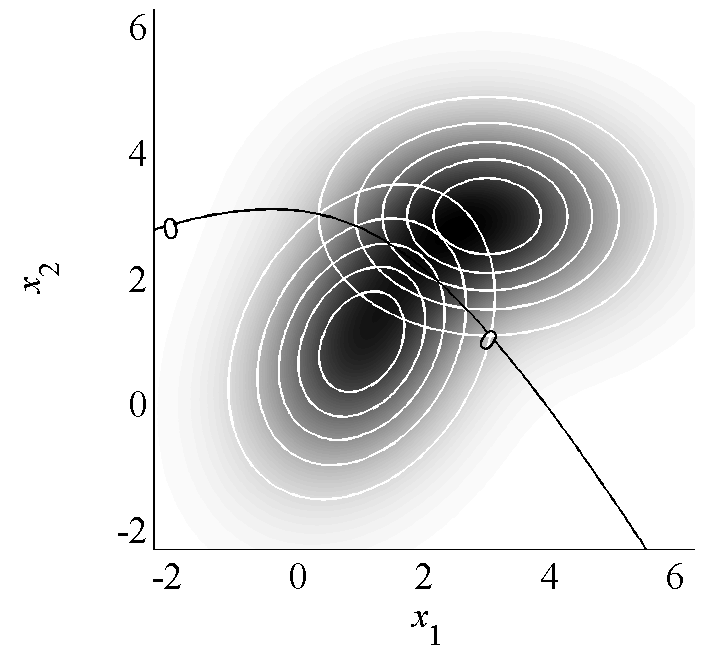
\includegraphics[width=6cm]{Figures/DecGauss2Dhip}
			\caption{Hyperbolic decision boundary of the ML detector and likelihoods for a Gaussian detection problem with 2D observations.}
			\label{fig:DecGauss2Dhip}
		\end{center}
	\end{figure}
\end{example}

\begin{example}
	Figure \ref{fig:DecGauss2Delip} shows an equivalent figure that of the previous example, but for a problem with the following means and cross-covariance matrices:
		\begin{equation*}
	{\bf m}_0 =  \left(\begin{array}{l}  0\\0  \end{array}\right), {\bf V}_0 = 
	\left(\begin{array}{ll} 0.7 & 0 \\ 0 & 0.7 \end{array} \right),
	\end{equation*}
	and
	\begin{equation*}
	{\bf m}_1 = \left(\begin{array}{l}  0.2 \\ 0.4 \end{array}\right), {\bf V}_1 = 
	\left(\begin{array}{ll} 0.5 & 0 \\ 0 & 0.2 \end{array} \right).
	\end{equation*}
	In this case, the decision boundary is an ellipse.
	\begin{figure}[htb]
		\begin{center}
			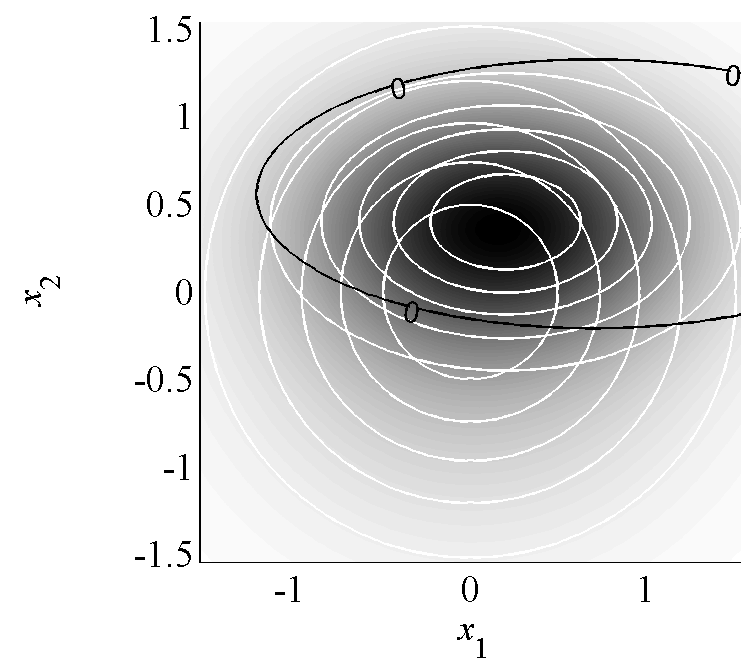
\includegraphics[width=6cm]{Figures/DecGauss2Delip.pdf}
			\caption{Elliptic decision boundary of the ML detectors and likelihoods for a Gaussian detection problem with 2D observations.}
			\label{fig:DecGauss2Delip}
		\end{center}
	\end{figure}
\end{example}

\subsubsection{Identical cross-covariance matrices}

This section considers the case of ${\bf V}_1 = {\bf V}_0 = {\bf V}$. Then, the LLRT becomes
\begin{equation*}
({\bf x}-{\bf m}_0)^T {\bf V}^{-1}({\bf x}-{\bf m}_0) 
- ({\bf x}-{\bf m}_1)^T {\bf V}^{-1}({\bf x}-{\bf m}_1)
\dunodcero \mu.
\end{equation*}
Now, expanding the quadratic forms, the above expression simplifies to
\begin{equation}
 ({\bf m}_1-{\bf m}_0)^T {\bf V}^{-1}{\bf x} \dunodcero \tilde{\mu},
 \label{eq:LLRT_Gaussian_same_Vs}
\end{equation}
where $\tilde{\mu} = \mu/2 + {\bf m}_1^T {\bf V}^{-1}{\bf m}_1/2 - {\bf m}_0^T {\bf V}^{-1}{\bf m}_0/2$. In this particular case, the LLRT in \eqref{eq:LLRT_Gaussian_same_Vs} is a linear function of the observation vector ${\bf x}$.

\begin{example}
	Figure \ref{Dec:DecGauss2Deqv} shows three decision boundaries for an example with
		\begin{equation*}
			{\bf m}_0 =  \left(\begin{array}{l}  1\\1  \end{array}\right), {\bf V}_0 = 
			\left(\begin{array}{ll} 0.44 & 0.32 \\ 0.32 & 0.81 \end{array} \right)
\end{equation*}
and
\begin{equation*}
{\bf m}_1 = \left(\begin{array}{l}  3\\3 \end{array}\right), {\bf V}_1 = 
\left(\begin{array}{ll} 0.44 & 0.32 \\ 0.32 & 0.81 \end{array} \right).
\end{equation*}
The label of each decision boundary is $\log(\eta)$. Then, $\log(\eta) = 0$ corresponds to the ML detector.
	\begin{figure}[htb]
		\begin{center}
			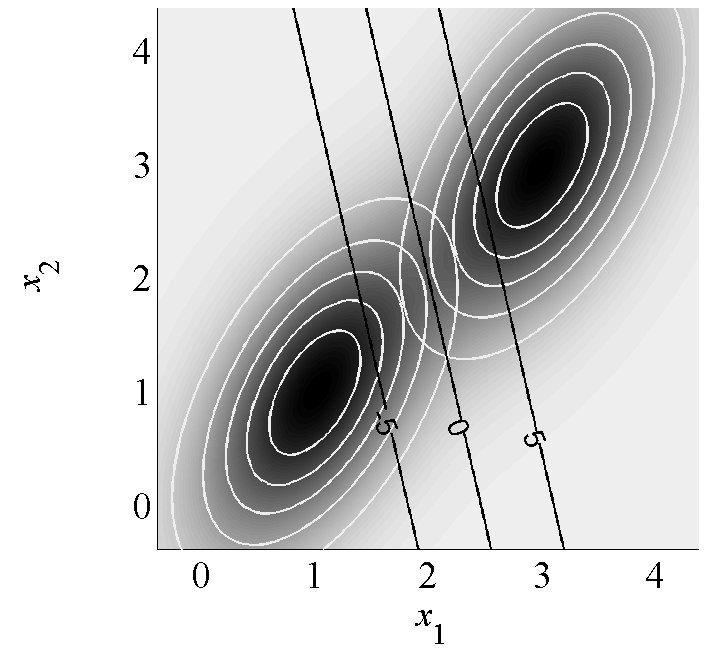
\includegraphics[width=6cm]{Figures/DecGauss2Deqv.pdf}
			\caption{Decision boundaries of the LLRT and likelihoods for a Gaussian detection problem with 2D observations and identical covariance matrices.}
			\label{Dec:DecGauss2Deqv}
		\end{center}
	\end{figure}
\end{example}

\begin{example}[Mathed filter]
	In this example, we derive one of the most well known detectors, the mathed filter (MF). The MF is the LLRT to the detection of a known signal contaminated by zero-mean Gaussian noise. Concretely, under hypothesis $h=0$, the observations are given by noise only:
	\begin{equation*}
	x[n] = w[n], \quad n = 0, \ldots, N-1,
	\end{equation*}
	and under  hypothesis $h=1$, the observations are
	\begin{equation*}
	x[n] = s[n] + w[n], \quad n = 0, \ldots, N-1,
	\end{equation*}
	where $s[n]$ is a known signal and $w[n]$ is additive white Gaussian noise with zero mean and variance $\sigma^2$, i.e., $w[n] \sim \Normal(0,\sigma^2)$. To use the LLRT already derived in this section, we must first define the vector
	\begin{equation*}
	{\bf x} = \begin{pmatrix} x[0] & x[1] & \cdots & x[N-1] \end{pmatrix}^T = {\bf s} + {\bf w},
	\end{equation*}
	with ${\bf s} = \begin{pmatrix} s[0] & s[1] & \cdots & s[N-1] \end{pmatrix}^T $ and ${\bf w} = \begin{pmatrix} w[0] & w[1] & \cdots & w[N-1] \end{pmatrix}^T$, and obtain the distributions of ${\bf x}$ under both hypothesis. Under hypothesis $h=0$, the observation vector ${\bf x}$ collects samples of a Gaussian process, which makes it also Gaussian. Hence, only the mean and cross-covariance matrices are required:
	\begin{equation*}
	{\bf m}_0 = \mathbb{E}\{{\bf x}|0\} = \mathbb{E}\{{\bf w}\} = \begin{pmatrix} \mathbb{E}\{w[0]\}  & \mathbb{E}\{w[1]\} & \cdots & \mathbb{E}\{w[N-1]\} \end{pmatrix}^T = \mathbf{0},
	\end{equation*}
    and
	\begin{align*}
		{\bf V}_0 &= \mathbb{E}\left\{({\bf x} - {\bf m}_0) ({\bf x} - {\bf m}_0)^T|0\right\} = \mathbb{E}\left\{{\bf w} {\bf w}^T\right\} \\ &= \mathbb{E}\left\{\begin{pmatrix} w[0] & w[1] & \cdots & w[N-1] \end{pmatrix}^T \begin{pmatrix} w[0] & w[1] & \cdots & w[N-1] \end{pmatrix}\right\} \\
		&= \begin{pmatrix} \mathbb{E}\left\{w^2[0]\right\}  & \mathbb{E}\left\{w[0]w[1] \right\}& \cdots & \mathbb{E}\left\{w[0]w[N-1]\right\} \\ \mathbb{E}\left\{w[1] w[0]\right\} & \mathbb{E}\left\{w^2[1]\right\} & \cdots & \mathbb{E}\left\{w[1]w[N-1]\right\} \\ \vdots & \vdots & \ddots & \vdots   \\ \mathbb{E}\left\{w[N-1] w[0]\right\} & \mathbb{E}\left\{w[N-1] w[1]\right\} & \cdots & \mathbb{E}\left\{w^2[N-1] \right\} \end{pmatrix}.
 	\end{align*}
	The cross-covariance matrix ${\bf V}_0$ can be simplified taking into account that the noise is white, i.e., $\mathbb{E}\{w[n] w[n-m]\} = \sigma^2 \delta[m]$, which yields 
	\begin{equation*}
		{\bf V}_0 = \begin{pmatrix} \sigma^2  & 0 & \cdots & 0 \\ 0 & \sigma^2 & \cdots & 0 \\ \vdots & \vdots & \ddots & \vdots   \\ 0 & 0 & \cdots & \sigma^2 \end{pmatrix} = \sigma^2 \mathbf{I}.
\end{equation*}
Similarly, under hypothesis $h=1$, the observations are Gaussian with mean
\begin{equation*}
	{\bf m}_1 = \mathbb{E}\{{\bf x}|1\} = \mathbb{E}\{{\bf s} + {\bf w}\} = \mathbb{E}\{{\bf s}\} + \mathbb{E}\{{\bf w}\} = {\bf s},
\end{equation*}
since ${\bf s}$ is deterministic, and cross-covariance matrix
	\begin{equation*}
{\bf V}_1 = \mathbb{E}\left\{({\bf x} - {\bf m}_1) ({\bf x} - {\bf m}_1)^T|1\right\} = \mathbb{E}\left\{({\bf s} + {\bf w} - {\bf s}) ({\bf s} + {\bf w} - {\bf s})^T\right\} = \mathbb{E}\left\{{\bf w} {\bf w}^T\right\} = \sigma^2 \mathbf{I}.
\end{equation*}
Hence, the detection problem is that of Gaussian observations with identical covariance matrices, for which the LLRT is
\begin{equation*}
({\bf m}_1-{\bf m}_0)^T {\bf V}^{-1}{\bf x} = \frac{1}{\sigma^2} {\bf s}^T {\bf x} \dunodcero \tilde{\mu} \Rightarrow \underbrace{\sum_{n = 0}^{N-1} s[n]x[n]}_{MF} \ \dunodcero \sigma^2 \tilde{\mu}.
\end{equation*}
Alternatively, and the motivation for the term matched filter, is because the above detector can be rewritten as a filtering of then signal $x[n]$ with the filter $h[n] = s[N-1 - n]$, followed by sampling every $N$ samples. Finally, we also would like to point out that the matched filter is a filter that maximizes the signal-to-noise ratio.

\end{example}

\subsubsection{Zero means}

We consider now that ${\bf m}_0 = {\bf m}_1 = \mathbf{0}$, which yields
\begin{equation*}
{\bf x}^T \left({\bf V}_0^{-1}-{\bf V}_1^{-1}\right){\bf x} \dunodcero \mu.
\label{eq:logLRTGauss2m0}
\end{equation*}

\begin{example}
	Figure \ref{fig:DecGauss2Deqm} shows the ML decision boundary for 2D Gaussian observations with
		\begin{equation*}
{\bf m}_0 =  \left(\begin{array}{l}  0\\0   \end{array}\right), {\bf V}_0 = 
\left(\begin{array}{ll} 0.62 & -0.22 \\ -0.22 & 0.37 \end{array} \right),
\end{equation*}
and
\begin{equation*}
{\bf m}_1 = \left(\begin{array}{l}  0\\0  \end{array}\right), {\bf V}_1 = 
\left(\begin{array}{ll} 1 & 0 \\ 0 & 2 \end{array} \right).
\end{equation*}
	The region ${\cal X}_0$ is given by the interior of the ellipse. Moreover, since the variance of the observations in every direction is larger under hypothesis $h=1$, points further away from the origin should be assigned $d=1$.
	\begin{figure}[htb]
		\begin{center}
			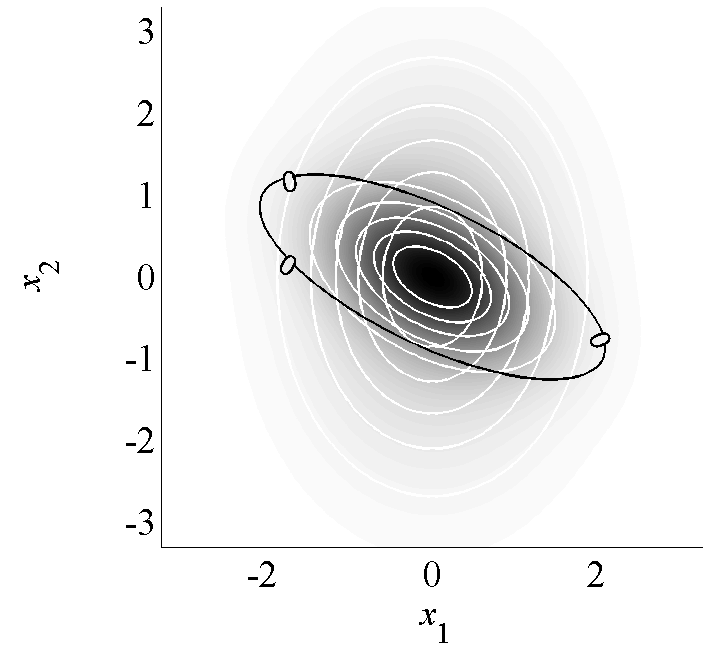
\includegraphics[width=6cm]{Figures/DecGauss2Deqm.pdf}
			\caption{Elliptic decision boundary for a 2D Gaussian problem with zero means.}
			\label{fig:DecGauss2Deqm}
		\end{center}
	\end{figure}
\end{example}

\begin{example}
	Figure \ref{fig:DecGauss2Deqm2} shows the ML decision boundary for 2D Gaussian observations with
	\begin{equation*}
	{\bf m}_0 =  \left(\begin{array}{l}  0\\0   \end{array}\right), {\bf V}_0 = 
	\left(\begin{array}{ll} 0.33 & 0.39 \\ 0.39 & 0.77  \end{array} \right)
	\end{equation*}
	and
	\begin{equation*}
	{\bf m}_1 = \left(\begin{array}{l}  0\\0  \end{array}\right), {\bf V}_1 = 
	\left(\begin{array}{ll} 0.39 &-0.19 \\ -0.19 & 0.16\end{array} \right).
	\end{equation*}
	In this example, the variance under hypothesis $h=1$ is larger only along dimension 1, whereas it is smaller along dimension 2. Hence, as a consequence, the boundary is a hyperbola.
	\begin{figure}[htb]
		\begin{center}
			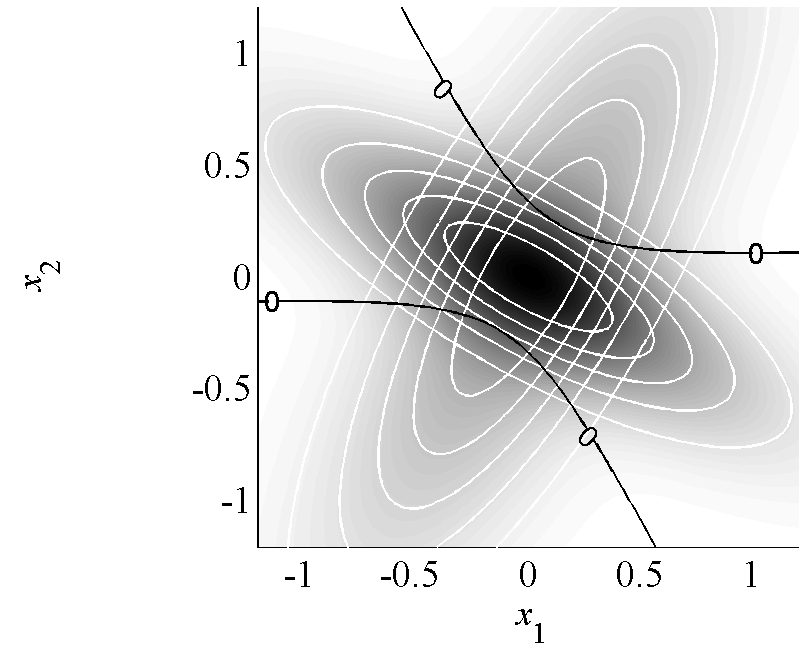
\includegraphics[width=6cm]{Figures/DecGauss2Deqm2.pdf}
			\caption{Hyperbolic decision boundary for a 2D Gaussian problem with zero means.}
			\label{fig:DecGauss2Deqm2}
		\end{center}
	\end{figure}
\end{example}

%\subsection{Summary of most relevant expressions}
%\subsubsection{General case}
%\begin{itemize}
%    \item Probability of error
%    $$P_e = P(D\neq H) = 1 - P(D=H)$$
%    \item Probability of error given ${\bf x}$
%    $$P(d\neq H|{\bf x}) = 1 - P(d = H|{\bf x}) = 1 - P_{H|{\bf X}}(d|{\bf x})$$
%    \item Mean cost
%    $$\mathbb{E}\left\{ c_{DH}\right\} = \sum_{h=0}^{M-1} \sum_{d=0}^{M-1} c_{dh} P(D=d, H=h)$$
%    \item Mean cost given $\bf x$
%    $$\mathbb{E}\left\{ c_{dH}\right|{\bf x}\} = \sum_{h=0}^{M-1} c_{dh} P_{H|X}(h|{\bf x})$$
%    \item ML classifier
%    $$d_{ML} = \arg\max_h p_{{\bf X}|H}({\bf x}|h)$$
%    \item MAP classifier
%    $$d_{MAP} = \arg\max_h P_{H|{\bf X}}(h|{\bf x})$$
%    \item Minimum mean cost classifier
%    $$d^\star = \arg\min_{d} \sum_{h=0}^{M-1} c_{dh} P_{H|X}(h|{\bf x})$$
%\end{itemize}
%
%\subsubsection{Binary case}
%\begin{itemize}
%    \item Probability of error
%    $$P_e = P_\text{M} P_H(1) + P_\text{FA} P_H(0)$$
%    \item Probability of False Alarm, Missing and Detection
%    \begin{align}
%        P_\text{FA} & = P(D=1|H=0) = \int_{{\cal X}_1} p_{\bf X|H}({\bf x}|0) d{\bf x} \nonumber \\
%        P_\text{M} & = P(D=0|H=1) = \int_{{\cal X}_0} p_{\bf X|H}({\bf x}|1) d{\bf x} \nonumber \\
%        P_\text{D} & = P(D=1|H=1) = 1 - P_\text{M} \nonumber
%    \end{align}
%    \item Likelihood ratio test:
%    $$\displaystyle\frac{p_{{\bf X}|H}({\bf x}|1)}{p_{{\bf X}|H}({\bf x}|0)} \dunodcero \eta$$
%    Some particular cases are:
%    \begin{itemize}
%        \item ML classifier: $\eta_{ML} = 1$
%        \item MAP classifier: $\eta_{MAP} = \displaystyle\frac{P_H(0)}{P_H(1)}$
%        \item Minimum mean cost classifier: $\eta^\star = \displaystyle\frac{c_{10}-c_{00}}{c_{01}-c_{11}} \displaystyle\frac{P_H(0)}{P_H(1)}$
%    \end{itemize}
%
%\end{itemize}

\chapter{Sequential Detection}
\label{sec:seq_det}
\section{Some introductory examples}

The previous chapter considered detection problems where we are given a set of observations and, based on them, we have to infer (decide) which hypothesis is true. Concretely, we have studied how to design the optimal detector (according to some criterion: maximum likelihood, minimum expected cost, etc.) and how to analyze its performance (false alarm and detection probabilities, error probability or average cost). 

In this chapter, we will study a different approach to detection problems, where the observations arrive sequentially and, moreover, we can decide whether we want to acquire more observations to achieve the desired performance. These problems are referred to as sequential detection problems, where the objective is to take a decision as soon as possible (acquiring the smallest amount of observations), while ensuring the required performance. 

In the following, we will study the problem of sequential detection in a simple set-up where there are only two hypotheses whose likelihoods are perfectly known, and the observations are independent and identically distributed (i.i.d.). But before we address the problem in a formal manner, this section presents two simple examples to introduce it. Concretely, we consider examples with and without gathering costs.

\subsection{Example 1: Sequential detection with no gathering cost}

Here, we present a simple example to motivate the problem of sequential detection. Consider an experiment in which the observation at time $n$ under hypothesis $H = 0$ follows a zero-mean Gaussian distribution with variance $\sigma^2 = 1$, and under hypothesis $H = 1$, the observation follows a zero-mean Gaussian distribution with variance $\sigma^2 = 4$. That is, the likelihoods are
\begin{equation}
	\label{eq:likelihood_0}
	p_{X[n] | H} (x[n] | 0) = \frac{1}{\sqrt{2 \pi}} \exp \left(-\frac{x^2[n]}{2}\right),
\end{equation}
and
\begin{equation}
	\label{eq:likelihood_1}
	p_{X[n] | H} (x[n] | 1) = \frac{1}{\sqrt{8 \pi}} \exp \left(-\frac{x^2[n]}{8}\right),
\end{equation}
which are shown in Figure \ref{fig:likelihoods_sequential}. Moreover, we assume that the observations are i.i.d.

\begin{figure}[t]
	\pgfmathsetmacro{\mypi}{3.141592}
	\begin{center}
		\begin{tikzpicture}
			\begin{axis}[%
				axis x line=middle,
				axis y line=middle,
				enlarge x limits=0.05,
				enlarge y limits=0.2,
				% xtick={-\mypi,-2*\mypi/\windowlength,2*\mypi/\windowlength,\mypi},
				% xticklabels={$-\pi$,$-\frac{2\pi}{N}$,$\frac{2\pi}{N}$,$\pi$},
				xmin=-6,
				xmax=6,
				ymin=0,
				%ytick=\empty,
				width=10cm,
				height=7.5cm,
				domain = -6:6,
				samples = 512,
				xlabel={$x[n]$},
				ylabel={$p_{X[n] | H} (x[n] | h) $}]
				\addplot[blue,thick] {1/sqrt(2*\mypi)*exp(-x^2/2)};
				\addplot[red,thick,dashed] {1/sqrt(8*\mypi)*exp(-x^2/8)};
				\legend{$h = 0$,$h = 1$};
			\end{axis}
		\end{tikzpicture}
	\end{center}
	\caption{Likelihoods considered in the introductory example}
	\label{fig:likelihoods_sequential}
\end{figure}

We shall start by considering no observations, $n = 0$, and derive the detector with minimum average cost and its cost. Concretely, considering $c_{00} = c_{11} = 0$ and $c_{01} = c_{10} = 1$, the minimum expected cost detector optimizes the cost
\begin{align*}
	\overline{C}_0 &= \mathbb{E}\{c_{DH}\} \\ &= c_{10} P(D = 1, H = 0) +  c_{01} P(D = 0, H = 1)  + c_{00} P(D = 0, H = 0) +  c_{11} P(D = 1, H = 1)  \\
	&= P(D = 1, H = 0) +  P(D = 0, H = 1) \\ &= P(D = 1 | H = 0) P_H(0) +  P(D = 0 |H = 1) P_H(1)
	\\ &= P(D = 1 | H = 0) p +  P(D = 0 |H = 1) (1 - p),
\end{align*}
where we have defined, for the sake of notation, $P_H(0) = p$ and $P_H(1) = 1 - p$. The probabilities $P(D = 1 | H = 0)$ and $P(D = 0 | H = 1)$ are determined by the detector. However, since there are no observations, the detector must always decide the same hypothesis, making one of the aforementioned probabilities one and the other zero. Then, for $0 \leq p \leq 1/2$, we should always decide $D = 1$, which yields $P(D = 1 | H = 0) = 1$, $P(D = 0 | H = 1) = 0$, and
\begin{equation*}
	\overline{C}_0 = p.
\end{equation*}
If we had decided always $D = 0$, we would have $P(D = 1 | H = 0) = 0$, $P(D = 0 | H = 1) = 1$, and
\begin{equation*}
	\overline{C}_0 = 1 - p,
\end{equation*}
which is obviously larger than $\overline{C}_0 = p$ for $0 \leq p \leq 1/2$. Similarly, for $1/2 < p \leq 1$, we should always decide $d = 0$, which implies that $P(D = 1 | H = 0) = 0$, $P(D = 0 | H = 1) = 1$, and
\begin{equation*}
	\overline{C}_0 = 1 - p.
\end{equation*}
Combining both results, the minimum average cost for varying $p$ is
\begin{equation*}
	\overline{C}_0(p) = \begin{cases} p, & 0 \leq p \leq 1/2, \\ 1 - p, & 1/2 < p \leq 1, \end{cases}
\end{equation*}
where we have explicitly written the dependence of the minimum average cost  with $p$. Figure \ref{fig:average_cost_n0} shows $\overline{C}_0(p)$ for varying $p$.

\begin{figure}[t]
	\begin{center}
		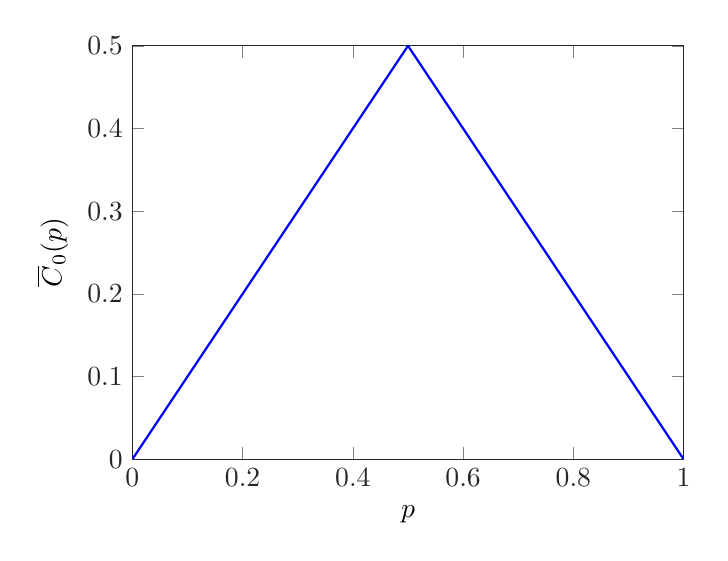
\begin{tikzpicture}
			\begin{axis}[%
				width=7cm,
				height=5.25cm,
				scale only axis,
				separate axis lines,
				every outer x axis line/.append style={white!15!black},
				every x tick label/.append style={font=\color{white!15!black}},
				xmin=0,
				xmax=1,
				xlabel={$p$},
				every outer y axis line/.append style={white!15!black},
				every y tick label/.append style={font=\color{white!15!black}},
				ymin=0,
				ymax=0.5,
				ylabel={$\overline{C}_0(p)$},
				legend style={draw=white!15!black,fill=white,legend cell align=left,legend pos=south east},
				]
				\addplot[blue,thick,domain=0:0.5,samples = 512] {x};
				\addplot[blue,thick,domain=0.5:1,samples = 512] {1 - x};
			\end{axis}
		\end{tikzpicture}
	\end{center}
	\caption{Minimum average cost with no observations}
	\label{fig:average_cost_n0}
\end{figure}

Let us now consider an arbitrary number of observations $n$, with $n >0$, and derive again the minimum expected cost detector, which minimizes the expected cost. This cost is denoted by $\overline{C}_n(p)$, to highlight that it depends on the number of observations and the prior probability $p$. Before proceeding, let us define $\mathbf{x}_n = (x[1], \ldots, x[n])^T$ as the vector that contains all available observations. Now, the sought detector is given by the likelihood ratio test (LRT), that is,
\begin{equation*}
	\frac{p_{{\bf X}_n|H}({\bf x}_n|1)}{p_{{\bf X}_n|H}({\bf x}_n|0)}\dunodcero \frac{c_{10}-c_{00}}{c_{01}-c_{11}} \frac{P_H(0)}{P_H(1)} = \frac{p}{1 - p}.
\end{equation*}
To compute the likelihood of the $n$ observations, we can use the i.i.d. assumption and, therefore,
\begin{equation*}
	p_{{\bf X}_n|H}({\bf x}_n|h) = \prod_{i = 1}^{n} p_{X[i]|H}( x[i] | h).
\end{equation*}
Using the likelihoods in \eqref{eq:likelihood_0} and \eqref{eq:likelihood_1}, we get
\begin{equation*}
	p_{{\bf X}_n|H}({\bf x}_n|0) = \prod_{i = 1}^{n} p_{X[i]|H}( x[i] | 0) = \prod_{i = 1}^{n} \frac{1}{\sqrt{2 \pi}} \exp \left(-\frac{x^2[i]}{2}\right) = \frac{1}{(2 \pi)^{n/2}} \exp \left(-\frac{1}{2} \sum_{i = 1}^{n} x^2[i]\right),
\end{equation*}
and
\begin{equation*}
	p_{{\bf X}_n|H}({\bf x}_n|1) = \prod_{i = 1}^{n} p_{X[i]|H}( x[i] | 1) = \prod_{i = 1}^{n} \frac{1}{\sqrt{8 \pi}} \exp \left(-\frac{x^2[i]}{8}\right) = \frac{1}{(8 \pi)^{n/2}} \exp \left(-\frac{1}{8} \sum_{i = 1}^{n} x^2[i]\right).
\end{equation*}
Then, the LRT becomes
\begin{equation*}
	\frac{\frac{1}{(8 \pi)^{n/2}} \exp \left(-\frac{1}{8} \sum_{i = 1}^{n} x^2[i]\right)}{\frac{1}{(2 \pi)^{n/2}} \exp \left(-\frac{1}{2} \sum_{i = 1}^{n} x^2[i]\right)} = \frac{1}{2^{n}} \exp \left(\frac{3 }{8} \sum_{i = 1}^{n} x^2[i]\right) \dunodcero \frac{p}{1 - p},
\end{equation*}
and the log-likelihood ratio test (LLRT) is
\begin{equation*}
  \frac{1}{n} \sum_{i = 1}^{n} x^2[i] \dunodcero \frac{8}{3} \left[\frac{1}{n} \log \left(\frac{p}{1 - p}  \right) + \log 2 \right].
\end{equation*}
Essentially, the LLRT compares the estimated variance with a threshold. The decision regions of the LLRT are
\begin{equation*}
	{\cal X}_1 = \left\{\x_n \in \mathbb{R}^{n} \left| \frac{1}{n} \sum_{i = 1}^{n} x^2[i]  >  \frac{8}{3} \left[ \frac{1}{n}  \log \left(\frac{p}{1 - p}  \right) + \log 2 \right] \right. \right\},
\end{equation*}
and
\begin{equation*}
	{\cal X}_0 = \left\{\x_n \in \mathbb{R}^{n} \left| \frac{1}{n} \sum_{i = 1}^{n} x^2[i]  \leq \frac{8}{3} \left[ \frac{1}{n}  \log \left(\frac{p}{1 - p}  \right) + \log 2 \right] \right. \right\}.
\end{equation*}
For these decision regions, we can compute the minimum expected cost as
\begin{align*}
	\overline{C}_n &= P(D = 1 | H = 0) p +  P(D = 0 |H = 1) (1 - p) \\
	&= p P_{\text{FA}} + (1 - p) P_{\text{M}},
\end{align*}
where
\begin{equation*}
	P_{\text{FA}} = P(D = 1 | H = 0) = \int_{{\cal X}_1} P_{{\bf X}_n|H}({\bf x}_n|0) d {\bf x}_n,
\end{equation*}
and
\begin{equation*}
	P_{\text{M}} = P(D = 0 | H = 1) = \int_{{\cal X}_0} P_{{\bf X}_n|H}({\bf x}_n|1) d {\bf x}_n.
\end{equation*}
Both, $P_{\text{FA}}$ and $P_{\text{M}}$, are given by complicated multidimensional integrals with no closed-form solution and that are difficult to evaluate numerically. Hence, we must compute them using a different approach.

We shall start by considering a transformation of the random variables $y[i], i = 1, \ldots, I$, which are Gaussian distributed with zero mean, unit variance, and i.i.d. Concretely, the transformation is
\begin{equation*}
	Z = \sum_{i = 1}^{I} y^2[i],
\end{equation*}
which is distributed as a Chi-squared random variable with $I$ degrees of freedom, denoted as $Z \sim \chi^2_{I}$. The probability density function of $Z$ is
\begin{equation*}
	p_Z(z) = \begin{cases} \frac{1}{2^{I/2} \Gamma(I/2)} z^{I/2 - 1} \exp(-z/2), & z >0, \\ 0, & \text{otherwise,} \end{cases}
\end{equation*}
and its cumulative distribution function is
\begin{equation*}
	F_Z(z) = \frac{\gamma(I/2,z/2)}{\Gamma(I/2)},
\end{equation*}
where $\Gamma(\cdot)$ is the gamma function and $\gamma(\cdot,\cdot)$ is the lower incomplete gamma function.\footnote{For positive integer values of the argument, the gamma function is given by $\Gamma(a) = (a - 1)!$. To compute the incomplete gamma function, it is necessary to resort to (uni-dimensional) numerical integration.} Figure \ref{fig:pdf_chi2} depicts $p_Z(z)$ and $F_Z(z)$ for a different number of degrees of freedom.

\begin{figure}[t]
	\begin{center}
		\includestandalone{Figures/Chi2_pdf} \includestandalone{Figures/Chi2_cdf}
	\end{center}
	\caption{Probability and cumulative density functions of a Chi-squared random variable with $I$ degrees of freedom}
	\label{fig:pdf_chi2}
\end{figure}

Using the Chi-squared distribution, we can compute $P_{\text{FA}}$ and $P_{\text{M}}$. The former is given by
\begin{align*}
	P_{\text{FA}} &= P(D = 1 | H = 0) \\ 
	&= P \left(\left. \frac{1}{n} \sum_{i = 1}^{n} x^2[i]  > \frac{8}{3} \left[ \frac{1}{n}  \log \left(\frac{p}{1 - p}  \right) + \log 2 \right] \right| H = 0 \right) \\ 
	&= P \left(\left. \sum_{i = 1}^{n} x^2[i]  > \frac{8}{3} \left[\log \left(\frac{p}{1 - p}  \right) + n \log 2 \right] \right| H = 0 \right),
\end{align*}
and taking into account that, under $H = 0$, $x[i]$ are i.i.d. Gaussian variables with zero mean and unit variance, $P_{\text{FA}}$ is the probability that a $\chi^2_n$ random variable is larger than $8/3 \left[\log \left(p/(1 - p)  \right) + n \log 2\right]$. That is,
\begin{equation*}
	P_{\text{FA}} = 1 - \frac{\gamma \left(n/2,\frac{8}{3} \left[\log \left(\frac{p}{1 - p}\right) + n \log 2 \right]\right)}{\Gamma(n/2)}.
\end{equation*}
We can proceed similarly for $P_{\text{M}}$ as follows
\begin{align*}
	P_{\text{M}} &= P(D = 0 | H = 1) \\ 
	&= P \left(\left. \frac{1}{n} \sum_{i = 1}^{n} x^2[i]  \leq \frac{8}{3} \left[ \frac{1}{n}  \log \left(\frac{p}{1 - p}  \right) + \log 2 \right] \right| H = 1 \right) \\ 
	&= P \left(\left. \sum_{i = 1}^{n} \left(\frac{x[i]}{2}\right)^2  \leq \frac{2}{3} \left[\log \left(\frac{p}{1 - p}  \right) + n \log 2 \right] \right| H = 1 \right).
\end{align*}
Under $H = 1$, $x[i]/2$ are i.i.d. Gaussian variables with zero mean and unit variance, and $P_{\text{M}}$ is therefore the probability that a $\chi^2_n$ random variable is smaller than $2/3 \left[\log \left(p/(1 - p)  \right) + n \log 2\right]$, which can be expressed as
\begin{equation*}
	P_{\text{M}} = \frac{\gamma \left(n/2,\frac{2}{3} \left[\log \left(\frac{p}{1 - p}  \right) + n \log 2 \right]\right)}{\Gamma(n/2)}.
\end{equation*}
\begin{figure}[t]
	\begin{center}
		\includestandalone{Figures/Expected_Cost1}
	\end{center}
	\caption{Minimum average cost with $n$ observations}
	\label{fig:average_cost_n}
\end{figure}
Hence, the expected cost becomes
\begin{multline}
	\overline{C}_n(p) = p \left(1 - \frac{\gamma \left(n/2,\frac{8}{3} \left[\log \left(\frac{p}{1 - p}  \right) + n \log 2 \right]\right)}{\Gamma(n/2)}\right) \\ + (1 - p) \left(\frac{\gamma \left(n/2,\frac{2}{3} \left[\log \left(\frac{p}{1 - p}  \right) + n \log 2 \right]\right)}{\Gamma(n/2)}\right), \label{eq:cost_n_nogathering}
\end{multline}
Let us now point out that the second argument of $\gamma \left(\cdot, \cdot\right)$ is negative for
\begin{align*}
%	8/3 \left[\log \left(\frac{p}{1 - p}  \right) + n \log 2\right] < 0 \nonumber \\
%	\log \left(\frac{p}{1 - p}  \right) + n \log 2 < 0  \nonumber \\
%	\log 2^n > \log \left(\frac{1 - p}{p}  \right) \nonumber \\
%	2^n < \frac{1 - p}{p}  \nonumber \\
%	p 2^n < 1 - p   \nonumber \\
%	p (2^n + 1) < 1 \nonumber \\
	p < \frac{1}{2^n + 1},
\end{align*}
making the lower incomplete gamma function zero, which yields
\begin{equation*}
	\overline{C}_n(p) = p,
\end{equation*}
for $p < \frac{1}{2^n + 1}$.

Figure \ref{fig:average_cost_n} shows $\overline{C}_n(p)$ for some values of $n$, which shows that
\begin{equation*}
	\overline{C}_0(p)  \geq \overline{C}_1(p) \geq \cdots \geq \overline{C}_n(p) \geq \cdots
\end{equation*}
Then, we should keep acquiring samples as long as we can (larger $n$) and, as a consequence, get a smaller minimum average cost.

\subsection{Example 2: Sequential detection with gathering cost}

\begin{figure}[t]
	\begin{center}
		\includestandalone{Figures/Expected_Cost2}
	\end{center}
	\caption{Minimum average cost, including the gathering cost, with $n$ observations}
	\label{fig:average_cost2_n}
\end{figure}

The results of the previous example do not make a lot of sense as we should keep collecting samples forever if we are to minimize the minimum average cost. Actually, for $n \rightarrow \infty$ we have $\overline{C}_n(p) \rightarrow 0$, regardless of $p$. Intuitively, we should include a cost every time an observation is collected, which should include a gathering cost related to, i.e., power consumption of the acquisition and transmission devices, and a waiting cost. Let us go back to the previous example and repeat it considering that this gathering (and waiting) cost is $c_{G} = 0.05$.

Taking into account $c_{G}$ and $\overline{C}_n(p)$ derived in \eqref{eq:cost_n_nogathering}, the modified cost is given by
\begin{multline*}
	\overline{C}_{n,G}(p)  = p \left(1 - \frac{\gamma \left(n/2,\frac{8}{3} \left[\log \left(\frac{p}{1 - p}  \right) + n \log 2 \right]\right)}{\Gamma(n/2)}\right) \\ + (1 - p) \left(\frac{\gamma \left(n/2,\frac{2}{3} \left[\log \left(\frac{p}{1 - p}  \right) + n \log 2 \right]\right)}{\Gamma(n/2)}\right) + c_G \cdot n,
\end{multline*}
which is depicted in Figure \ref{fig:average_cost2_n}. From this figure, we can notice that keeping collecting samples does not necessarily improve $\overline{C}_{n,G}(p)$ as it happened in the case of no gathering cost, that is, $\overline{C}_{n,G}(p) \not \geq \overline{C}_{n+1,G}(p), \forall p \in [0,1]$. However, there is a range of values of $p$, for which it holds that $\overline{C}_{n,G}(p) \geq \overline{C}_{n+1,G}(p)$. Hence, sometimes it will be convenient to acquire an additional samples and sometimes it will not. Precisely this idea is the main ingredient of sequential detection.

\section{Sequential test}

We have used the previous examples to motivate sequential detection, but such story is not completely accurate because to derive the minimum expected cost at time $n$, the detector needs to use $n$ samples. However, we need to make the decision every time a new sample is acquired, which makes the story a bit simpler as we shall see.
 % what happens if  we had stopped earlier or what happens to the gathering cost of the previous time instants once we have already acquired those observations. In fact, the story is a bit simpler.

\begin{figure}[t]
	\begin{center}
		\includestandalone{Figures/Expected_Cost3}
	\end{center}
	\caption{Minimum average cost, including the gathering cost, with $n$ observations}
	\label{fig:average_cost3_n}
\end{figure}

Consider there are no observations available, that is $n = 0$. At this time instant, we need to decide between $H = 0$, $H = 1$, or take another sample. Since there are no available samples, the cost of always deciding $D = 1$ is $p$, the prior probability of $H = 0$, the cost of always deciding $D = 0$ is $1 - p$, the prior probability of $H = 1$, and the minimum expected cost with $n = 1$ sample is $\overline{C}_{1,G}(p)$. These three costs are depicted in Figure \ref{fig:average_cost3_n}, which shows that they intersect at two points. The first of these two points, $p_L$, can be obtained as the largest value of $p$ for which $\overline{C}_{1,G}(p)$ is still larger than the cost of always deciding $D = 1$. Mathematically, $p_L$ is obtained as
\begin{equation*}
	p_L = \sup_{p} \ \{p \mid \overline{C}_{1,G}(p) > p\}.
\end{equation*}
Similarly, $p_U$ is the smallest value of $p$ where $\overline{C}_{1,G}(p)$ starts to be larger than the cost of always deciding $D = 0$, that is,
\begin{equation*}
	p_U = \inf_{p} \  \{p \mid \overline{C}_{1,G}(p) > 1 - p\}.
\end{equation*}
Hence, for $p \in [0,p_L]$, with $p_L = 0.4057$ in our example, the cost of always deciding $D = 1$ is the smallest, whereas for $p \in [p_U,1]$, with $p_U = 0.7403$, the cost of always deciding $D = 0$ is the smallest. However, for $p \in (p_L,p_U)$, neither the cost of always deciding $D = 0$, nor the cost of always deciding $D = 1$ is the smallest, and we must take another sample. Summarizing, at time $n = 0$, the sequential test must\footnote{Although this sequential test was obtained for a particular example, it is a general result since $\overline{C}_{1,G}(p)$ is a concave function of $p$ in $[0,1]$ for any likelihood and any other costs $c_{DH}$ and $c_{G}$. Nevertheless, the derived values of $p_L$ and $p_U$ would be different.}
\begin{equation}
\label{eq:seq_test_n0}
\begin{array}{l}
	\text{decide } D = 1 \text{ for } p \leq p_L, \\
	\text{decide } D = 0 \text{ for } p \geq p_U, \\
	\text{take another sample for } p_L < p < p_U.
\end{array}
\end{equation}

The question that remains to be answered is: What do we have to do if we have decided to take another sample? To answer this question, we must note that at $n = 1$, we have already taken the sample, i.e., the gathering cost has been already spent. Moreover, the possible decisions at $n = 1$ are exactly those of $n = 0$: decide between $H = 0$, $H = 1$, or take another sample. That is, the effect of having already taken one sample does not modify the test as there are still an infinite number of available samples. However, there is one important difference. The value of $x[1]$ provides some (partial) knowledge about the hypothesis. Then, conditioned on having observed $x[1]$, we should repeat the sequential test in \eqref{eq:seq_test_n0}, but instead of using the prior probability $P(H = 0) = p$, we must use the posterior probability $P(H = 0 | X[1] = x[1]) = p_1$, i.e.,
\begin{equation*}
	\begin{array}{l}
		\text{decide } D = 1 \text{ for } p_1 \leq p_L, \\
		\text{decide } D = 0 \text{ for } p_1 \geq p_U, \\
		\text{take another sample for } p_L < p < p_U.
	\end{array}
\end{equation*}
Similarly, at a generic time $n$, the sequential test is
\begin{equation}
	\label{eq:seq_test}
	\begin{array}{l}
		\text{decide } D = 1 \text{ for } p_n \leq p_L, \\
		\text{decide } D = 0 \text{ for } p_n \geq p_U, \\
		\text{take another sample for } p_L < p < p_U,
	\end{array}
\end{equation}
where the posterior probability is now
\begin{equation*}
	p_n = P(H = 0 | X[1] = x[1], \ldots, X[n] = x[n]),
\end{equation*}
with $p_0 = P(H = 0) = p$. To conclude the derivation of the sequential test, we must find an explicit expression for $p_n$. First, using Bayes's theorem we can rewrite $p_n$ as
\begin{align*}
	p_n &= P(H = 0 | X[1] = x[1], \ldots, X[n] = x[n]) \\ &= \frac{P(H = 0 , X[1] = x[1], \ldots, X[n] = x[n])}{P(X[1] = x[1], \ldots, X[n] = x[n])} \\ &= \frac{P(X[1] = x[1], \ldots, X[n] = x[n] | H = 0) P_H(0)}{P(X[1] = x[1], \ldots, X[n] = x[n])}.
\end{align*}
Applying now the law of total probability to the denominator, $p_n$ becomes
\begin{align}
	p_n &= \frac{P(X[1] = x[1], \ldots, X[n] = x[n] | H = 0) P(H = 0)}{\displaystyle \sum_{h = 0}^{1} P(X[1] = x[1], \ldots, X[n] = x[n] | H = h) P_H(h)} \nonumber \\ &= 
	\frac{p_{\mathbf{X}_n | H}(\x_n | 0) p}{p_{\mathbf{X}_n | H}(\x_n | 0) p + p_{\mathbf{X}_n | H}(\x_n | 1) (1 - p)}, \label{eq:pn_pre}
\end{align}
which is a function of both likelihoods, $P_{\mathbf{X}_n | H}(\x_n | 0)$ and $P_{\mathbf{X}_n | H}(\x_n | 1)$, and $p$. Finally, taking into account the i.i.d. assumption, we can simplify \eqref{eq:pn_pre} as
\begin{equation}
	\label{eq:pn}
	p_n = \frac{p}{\displaystyle p +  (1 - p) \frac{p_{\mathbf{X}_n | H}(\x_n | 1)}{p_{\mathbf{X}_n | H}(\x_n | 0)}} = \frac{p}{\displaystyle p +  (1 - p) \prod_{i = 1}^{n} \frac{p_{X[i] | H}(x[i] | 1)}{p_{X[i] | H}(x[i] | 0)}},
\end{equation}
where, for the sake of consistency, we define $\prod_{i = 1}^{0} = 1$.

Finally, and continuing with our example, where
\begin{equation*}
	\frac{p_{X[i] | H}(x[i] | 1)}{p_{X[i] | H}(x[i] | 0)} = \frac{1}{2} \exp \left(\frac{3 }{8} x^2[i] \right), \ i = 1, 2, \ldots,
\end{equation*}
Figure \ref{fig:seq_test_realizations} shows several realizations of the sequential test in \eqref{eq:seq_test} for this example, when $p = 0.5$. Some of these realizations were obtained for $x[n]$ generated under $H = 0$ and other realizations for  $x[n]$ generated under $H = 1$. In this figure, we can see that as soon as $p_n$ is above $p_U$ or below $p_L$, the detector stops the acquisition of more observations. In the former case, the decision is $D = 0$, whereas in the latter, it is $D = 1$.
\begin{figure}[t]
	\begin{center}
		\includestandalone{Figures/seq_test_realizations}
	\end{center}
	\caption{Realizations of the sequential test}
	\label{fig:seq_test_realizations}
\end{figure}

\section{Sequential probability ratio test}

Using \eqref{eq:pn}, the sequential test in \eqref{eq:seq_test} is
\begin{equation}
	\label{eq:seq_SPRT_mincost}
	\begin{array}{l}
		\text{decide } D = 1 \text{ for } \phi_n \geq \frac{p (1 - p_L)}{p_L(1 - p)}, \\
		\text{decide } D = 0 \text{ for } \phi_n \leq  \frac{p (1 - p_U)}{p_U (1 - p)}, \\
		\text{take another sample for } \frac{p (1 - p_U)}{p_U (1 - p)} < \phi_n < \frac{p (1 - p_L)}{p_L(1 - p)},
	\end{array}
\end{equation}
where
\begin{equation*}
	\phi_n = \prod_{i = 1}^{n} \frac{p_{X[i] | H}(x[i] | 1)}{p_{X[i] | H}(x[i] | 0)}.
\end{equation*}
% \begin{align}
%	 \eta_U &= \frac{p (1 - p_L)}{p_L(1 - p)},  & \eta_L &= \frac{p (1 - p_U)}{p_U (1 - p)}. \label{eq:eta_mincost}
%\end{align}
Then, the sequential test boils down to a likelihood ratio test, and it is therefore named the sequential probability ratio test (SPRT). Note that the SPRT can be computed recursively when a new observation comes in, i.e.,
\begin{equation*}
	\phi_n = \prod_{i = 1}^{n} \frac{P_{X[i] | H}(x[i] | 1)}{P_{X[i] | H}(x[i] | 0)} = \left(\prod_{i = 1}^{n-1} \frac{P_{X[i] | H}(x[i] | 1)}{P_{X[i] | H}(x[i] | 0)}\right) \frac{P_{X[n] | H}(x[n] | 1)}{P_{X[n] | H}(x[n] | 0)} = \phi_{n-1} \cdot \frac{P_{X[n] | H}(x[n] | 1)}{P_{X[n] | H}(x[n] | 0)},
\end{equation*}
with $\phi_0 = 1$.

Actually, \eqref{eq:seq_SPRT_mincost} is just one example of the SPRT for a particular choice of the thresholds (those that optimize the expected cost). The most general SPRT is given by
\begin{equation}
	\label{eq:seq_SPRT}
	\begin{array}{l}
		\text{decide } D = 1 \text{ for } \phi_n \geq \eta_U, \\
		\text{decide } D = 0 \text{ for } \phi_n \leq  \eta_L, \\
		\text{take another sample for } \eta_L < \phi_n < \eta_U,
	\end{array}
\end{equation}
where the thresholds should satisfy
\begin{equation*}
	0 < \eta_L < 1 < \eta_U < \infty.
\end{equation*}
Intuitively, for larger values of $\eta_U$, it is more unlikely to decide $D = 1$. This implies that it will take longer to decide $D = 1$, while at the same time, it will be more unlikely to decide $D = 1$ when $H = 0$. Similarly, for smaller values of $\eta_L$, it is more unlikely to decide $D = 0$ and, therefore, it will take longer to decide $D = 0$, while at the same time, it will be more unlikely to decide $D = 0$ when $H = 1$. These suggests that there are three metrics at play: the probability of false alarm ($\pfa = P(D = 1 | H = 0)$), the probability of missing ($\pmis = P(D = 0 | H = 1)$), and the sample size $N$, which is defined as
\begin{equation*}
	\label{eq:sample_size}
	N =  \min_{n} \ \{n \mid \phi_n \geq \eta_U \text{ or } \phi_n \leq \eta_L\}. 
\end{equation*}
Thus,  the most established objective is to design the SPRT, i.e., the thresholds $\eta_L$ and $\eta_U$ in \eqref{eq:seq_SPRT}, that minimizes $N$ while guaranteeing that $\pfa \leq \alpha$ and $\pmis \leq \beta$, where $\alpha$ and $\beta$ are the target values of probability of false alarm and probability of missing, respectively. In the following, we will derive $\pfa$ and $\pmis$ as a function of the thresholds.

Let us start by the probability of false alarm, which is defined as
\begin{equation*}
	\pfa = P(D = 1 | H = 0) = \int_{\mathcal{X}_1} p_{\mathbf{X}_{\infty} | H} (\mathbf{x}_{\infty} | 0) d \mathbf{x}_{\infty},
\end{equation*}
where $\mathbf{x}_{\infty} \in \mathbb{R}^{\infty}$ and
\begin{equation*}
	\mathcal{X}_1 = \{ \mathbf{x}_{\infty} \in \mathbb{R}^{\infty} | \phi_{N} \geq  \eta_U  \}.
\end{equation*}
To continue, we must note that the set $\mathcal{X}_1$ can be decomposed as
\begin{equation*}
	\mathcal{X}_1 = \mathop{\bigcup}\limits_{n = 1}^{\infty} \mathcal{X}_{1,n},
\end{equation*}
with
\begin{equation*}
	\mathcal{X}_{1,n} = \{ \mathbf{x}_{\infty} \in \mathbb{R}^{\infty} |N = n \text{ and } \phi_{n} \geq  \eta_U  \}.
\end{equation*}
That is, we decide $D = 1$ when we decide $D = 1$ at $n = 1$, or at $n = 2$, or at $n = 3$, $\ldots$ Moreover, taking into account that if we decide $D = 1$ at $n$, we could not decide it at a different time instant $m$, with $n \neq m$, the sets $\mathcal{X}_{1,n}$ and $\mathcal{X}_{1,m}$ are mutually exclusive, i.e., they do not overlap, allowing us to write
\begin{align*}
	\pfa &= \int_{\mathcal{X}_1} p_{\mathbf{X}_{\infty} | H} (\mathbf{x}_{\infty} | 0) d \mathbf{x}_{\infty} 
	= \int_{\cup_{n = 1}^{\infty} \mathcal{X}_{1,n}} p_{\mathbf{X}_{\infty} | H} (\mathbf{x}_{\infty} | 0) d \mathbf{x}_{\infty} 
	= \sum_{n = 1}^{\infty}  \int_{\mathcal{X}_{1,n}} p_{\mathbf{X}_{n} | H} (\mathbf{x}_{n} | 0) d \mathbf{x}_{n} \\
	&= \sum_{n = 1}^{\infty}  \int_{\mathcal{X}_{1,n}} \prod_{i = 1}^{n} p_{X[i] | H}(x[i] | 0)  d \mathbf{x}_{n}.
\end{align*}
Using now that
\begin{equation*}
	\phi_n \geq \eta_U \Rightarrow   \prod_{i = 1}^{n} p_{X[i] | H}(x[i] | 0) \leq \eta_U^{-1} \prod_{i = 1}^{n} p_{X[i] | H}(x[i] | 1)
\end{equation*}
for $\mathbf{x}_n \in \mathcal{X}_{1,n}$, we have 
\begin{equation*}
	\pfa \leq  \eta_U^{-1} \sum_{n = 1}^{\infty}  \int_{\mathcal{X}_{1,n}}  \prod_{i = 1}^{n} p_{X[i] | H}(x[i] | 1)  d \mathbf{x}_{n}.
\end{equation*}
Since the probability of detection is
\begin{align*}
	\pdet &= \int_{\mathcal{X}_1} p_{\mathbf{X}_{\infty} | H} (\mathbf{x}_{\infty} | 1) d \mathbf{x}_{\infty} 
	= \sum_{n = 1}^{\infty}  \int_{\mathcal{X}_{1,n}} \prod_{i = 1}^{n} p_{X[i] | H}(x[i] | 1)  d \mathbf{x}_{n} \\
	&= 1 - \pmis,
\end{align*}
we get
\begin{equation}
	\label{eq:bound_pfa}
	\pfa \leq  \eta_U^{-1} \left(1 - \pmis\right).
\end{equation}

To compute the probability of missing, it is possible to follow a similar approach. Define
\begin{equation*}
	\mathcal{X}_0 = \{ \mathbf{x}_{\infty} \in \mathbb{R}^{\infty} | \phi_{N} \leq  \eta_L  \} = \mathop{\bigcup}\limits_{n = 1}^{\infty} \mathcal{X}_{0,n},
\end{equation*}
where
\begin{equation*}
	\mathcal{X}_{0,n} = \{ \mathbf{x}_{\infty} \in \mathbb{R}^{\infty} |N = n \text{ and } \phi_{n} \leq  \eta_L  \}.
\end{equation*}
Hence, the probability of missing is
\begin{equation*}
	\pmis = P(D = 0 | H = 1) = \int_{\mathcal{X}_0} p_{\mathbf{X}_{\infty} | H} (\mathbf{x}_{\infty} | 1) d \mathbf{x}_{\infty} = \sum_{n = 1}^{\infty}  \int_{\mathcal{X}_{0,n}} \prod_{i = 1}^{n} p_{X[i] | H}(x[i] | 1)  d \mathbf{x}_{n}.
\end{equation*}
The above expression can be bounded as
\begin{equation*}
	\pmis \leq  \eta_L \sum_{n = 1}^{\infty}  \int_{\mathcal{X}_{0,n}}  \prod_{i = 1}^{n} p_{X[i] | H}(x[i] | 0)  d \mathbf{x}_{n},
\end{equation*}
since
\begin{equation*}
	\phi_n \leq \eta_L \Rightarrow   \prod_{i = 1}^{n} p_{X[i] | H}(x[i] | 1) \leq \eta_L \prod_{i = 1}^{n} p_{X[i] | H}(x[i] | 0),
\end{equation*}
for $\mathbf{x}_n \in \mathcal{X}_{0,n}$. Finally, we get
\begin{equation}
	\label{eq:bound_pm}
	\pmis \leq  \eta_L (1 - \pfa),
\end{equation}
where we have taken into account that
\begin{equation*}
	\sum_{n = 1}^{\infty}  \int_{\mathcal{X}_{0,n}}  \prod_{i = 1}^{n} p_{X[i] | H}(x[i] | 0)  d \mathbf{x}_{n} = 1 - \sum_{n = 1}^{\infty}  \int_{\mathcal{X}_{1,n}}  \prod_{i = 1}^{n} p_{X[i] | H}(x[i] | 0)  d \mathbf{x}_{n} = 1 - \pfa.
\end{equation*}

The bounds for the probabilities of false alarm and missing in \eqref{eq:bound_pfa} and \eqref{eq:bound_pm} allow us to obtain the values $\eta_L$ and $\eta_U$ that achieve the desired value for $P_{\text{FA}}$ and $P_{\text{M}}$. Concretely, we only need to solve the inequalities in \eqref{eq:bound_pfa} and \eqref{eq:bound_pm}, which yields
\begin{align*}
	\eta_L &\geq \frac{\pmis}{1 - \pfa},  &  \eta_U &\leq  \frac{1 - \pmis}{\pfa},
\end{align*}
which are, in fact, only bounds. To avoid the inequalities and derive (approximate) equalities, we need to assume that when $\phi_N$ crosses the boundaries $\eta_L$ and $\eta_U$, the excess over the boundaries is negligible. That is,
\begin{align*}
	\phi_N - \eta_U &\rightarrow \epsilon_1,  &  \eta_L - \phi_N &\rightarrow \epsilon_2,
\end{align*}
with $\epsilon_i$ arbitrarily small positive constants. Under these assumptions, which are very accurate for large $N$, we get 
\begin{align*}
	\eta_L &\approx \frac{\pmis}{1 - \pfa},  &  \eta_U &\approx  \frac{1 - \pmis}{\pfa},
\end{align*}
which are known as Wald's approximations. Interestingly, and contrary to what happens with the LRT, the thresholds required to achieve the desired probabilities of false alarm and missing do not depend on the likelihoods. Nevertheless, the SPRT does depend on the likelihoods, and so do the sample size, $N$, and the expected sample size, $\mathbb{E}\{N\}$.

We conclude the topic of sequential detection by presenting the Wald-Wolfowitz theorem. Let us denote the probabilities of false alarm and missing of the SPRT $\pfa(\phi)$ and $\pmis(\phi)$, and its sample size $N(\phi)$. Consider an alternative sequential decision rule with probabilities of false alarm and missing $\pfa(\psi)$ and $\pmis(\psi)$, which satisfy
\begin{align*}
	\pfa(\psi) &\leq \pfa(\phi), & \pmis(\psi) &\leq \pmis(\phi).
\end{align*}
Then, the Wald-Wolfowitz theorem states that
\begin{equation*}
	\mathbb{E} \{N(\psi)\} \geq \mathbb{E} \{N(\phi)\},
\end{equation*}
where $N(\psi)$ is the sample size of the alternative decision rule. Hence, for a desired level of performance ($\pfa \leq \alpha$ and $\pmis \leq \beta$), there does not exist any sequential decision rule that achieves an expected sample size smaller than that of the SPRT. Interestingly, since a fixed-sample-size detector can be seen as a (very particular) sequential decision rule, the average sample size of the SPRT can not be larger than the sample size of any fixed-sample-size detector  with the same level of performance. Alternatively, the Wald-Wolfowitz theorem also states that, for a fixed expected sample size, there is no sequential rule that achieves smaller $\pfa$ and $\pmis$ than those of the SPRT.
%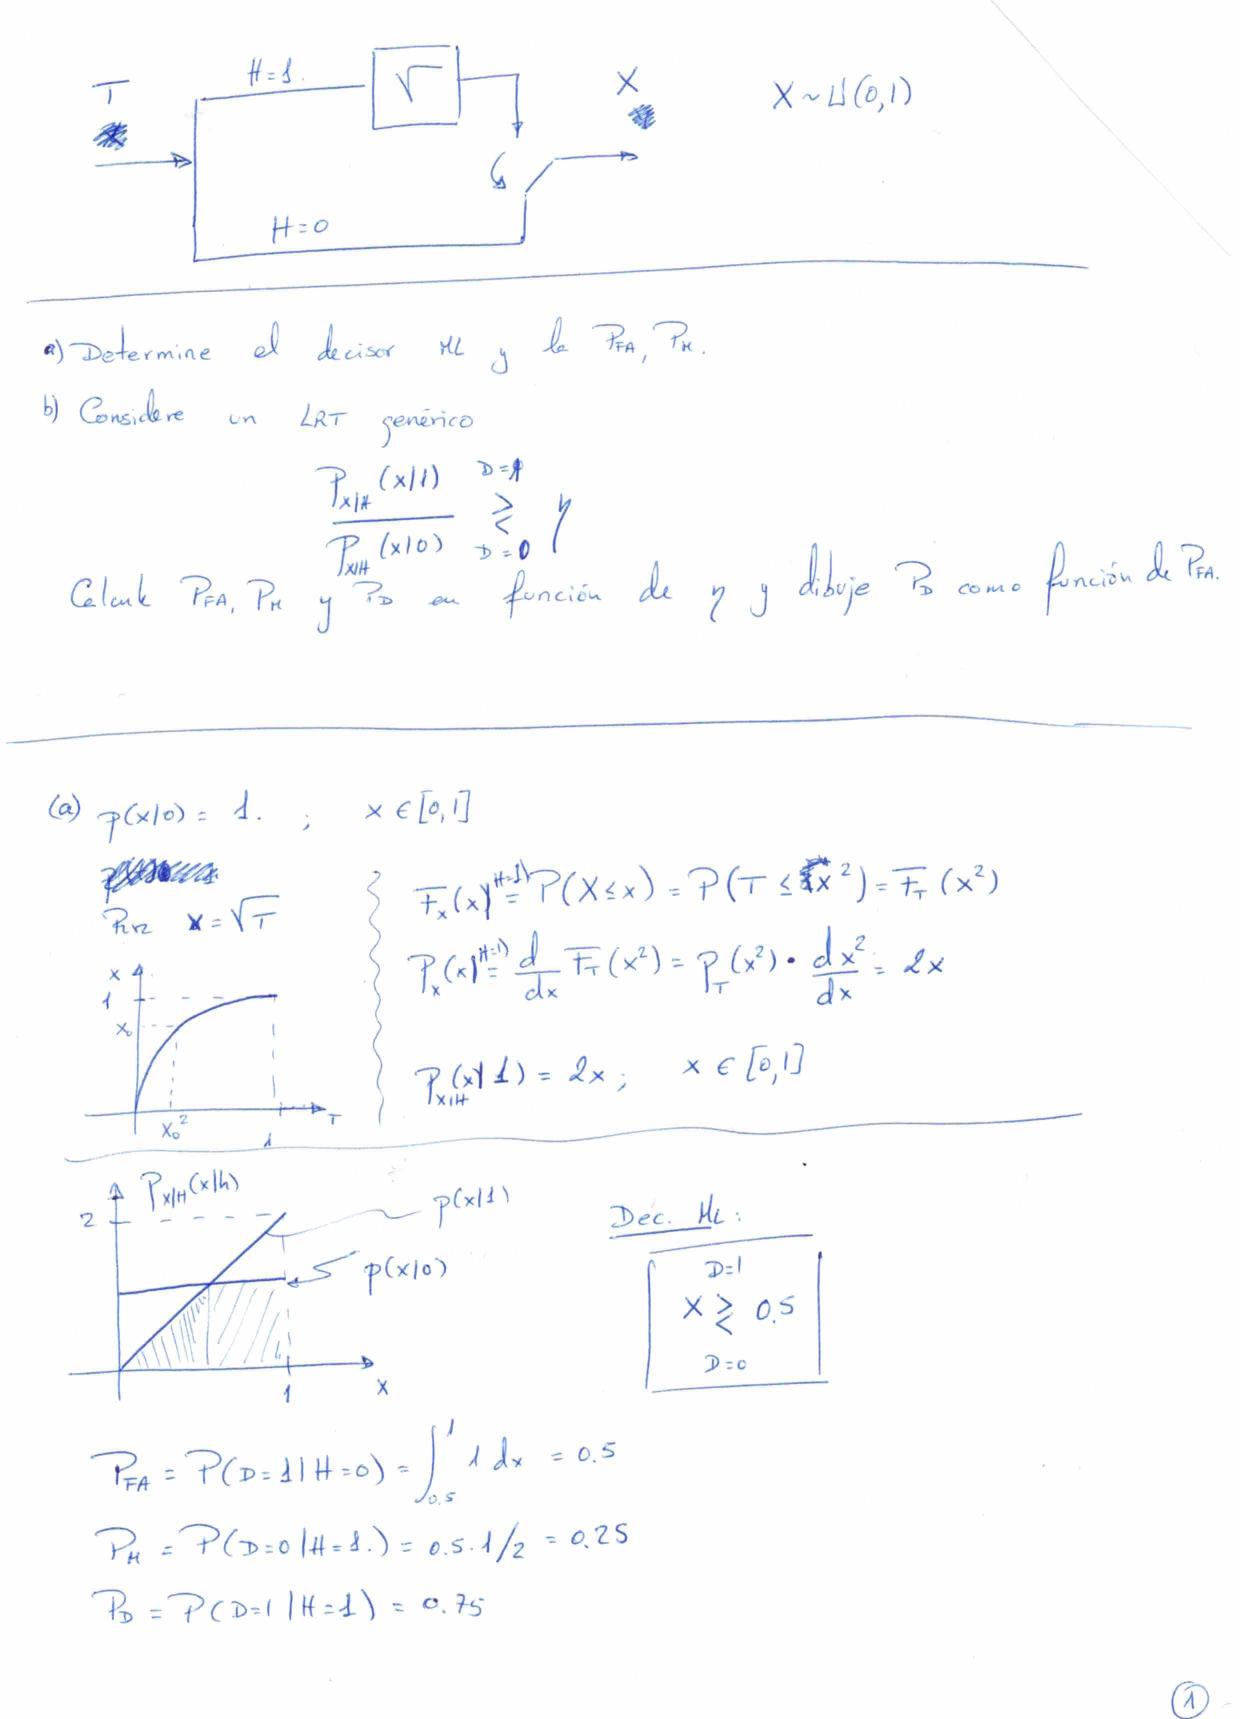
\includepdf[pages=-]{Contents/LRT_Labo_Clas_problem}

% Appendix
%%%%%%%%%%%%%%%%%%%%% appendix.tex %%%%%%%%%%%%%%%%%%%%%%%%%%%%%%%%%
%
% sample appendix
%
% Use this file as a template for your own input.
%
%%%%%%%%%%%%%%%%%%%%%%%% Springer-Verlag %%%%%%%%%%%%%%%%%%%%%%%%%%

\appendix
%\motto{All's well that ends well}
\chapter{Transformations of random variables}
\label{introA} % Always give a unique label
% use \chaptermark{}
% to alter or adjust the chapter heading in the running head

%%%%%%%%%%%%%%%%%%%%%%%%%%%%%%%%%%%
\section{Change of Random Variable}
\label{sec:1}
%%%%%%%%%%%%%%%%%%%%%%%%%%%%%%%%%%%

Let's consider we know the probability of a r.v. $X$, $\px$, and we now want to compute the probability density function of some variable $Y=f(X)$, that is, we need to calculate $\py$.

To understand how this new distribution or {\bf change of random variable} is calculated, let's firstly solve a particular case:

\begin{itemize}
\item $X$ is a uniform distribution in the interval $(0,1)$.

\begin{center}
\begin{tabular}{m{.5\textwidth}m{.4\textwidth}}
 \begin{equation} 
\px = \begin{cases}
1 & {\rm if} \quad 0<x<1\\
0 & {\rm otherwise} 
\end{cases} \nonumber
\end{equation} & 
\raisebox{-8ex}{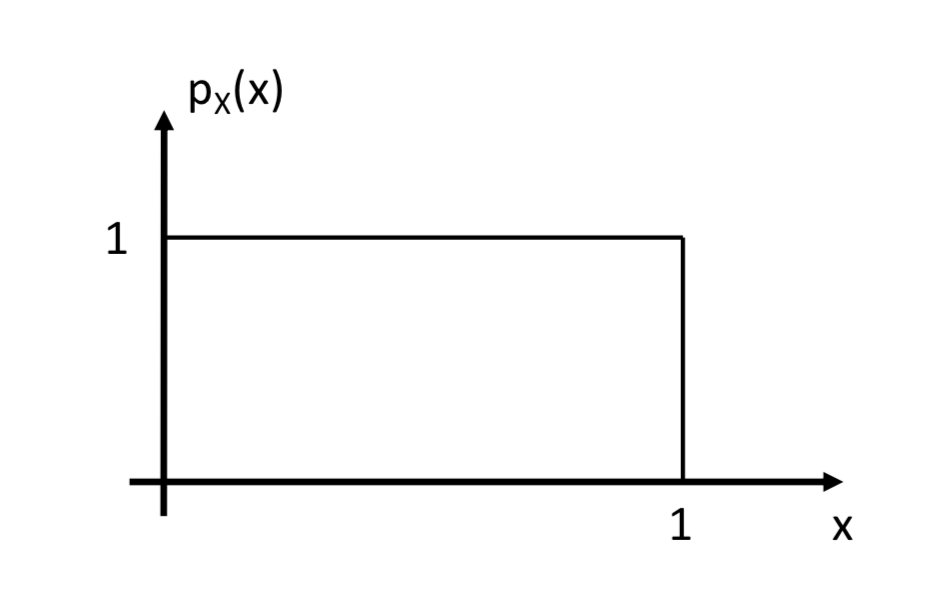
\includegraphics[scale=.25]{Figures/Fig11.png}} \\ 
\end{tabular}
\end{center}

\item $Y = X^2$. Note that this change produces this transformation:
\begin{center}
\begin{tabular}{m{.5\textwidth}m{.4\textwidth}}
 \raisebox{-8ex}{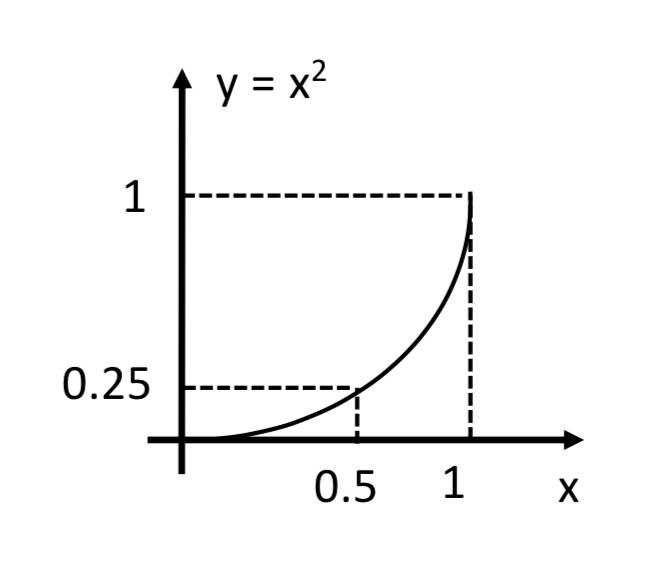
\includegraphics[scale=.4]{Figures/Fig12.png}} &
 \begin{tabular}{l|l}
$x$ & $y = x^2$ \\ \hline
0.1 & 0.01\\
0.2 & 0.04\\
0.5 & 0.25\\
... & ...\\
\end{tabular} 
\end{tabular}
\end{center}

The transformation function $f(\cdot)$ is strictly increasing. So there exists its inverse function $f^{-1}(\cdot)$.

\end{itemize}
To solve this change of r.v., we are going to use the fact that:

\begin{eqnarray}
P\{0<X<0.1\} &  = & P\{0<Y<0.01\}  \nonumber\\
P\{0<X<0.2\} &  = & P\{0<Y<0.04\}  \nonumber\\
P\{0<X<0.5\} &  = & P\{0<Y<0.25\}  \nonumber
\end{eqnarray}
or, in a general case, for any value of $X$, $x_0$, we have
$$ P\{0<X<x_0\}  = P\{0<Y<y_0\}$$
where $y_0=x_0^2$ or $x_0= \sqrt{y_0}$ 

So, we can compute the cumulative distribution function of the r.v. $Y$ as
$$ F_Y(y_0) =  P\{Y<y_0\} =  P\{X<\sqrt{y_0}\}$$

Now, as the cumulative function of $Y$ is expressed in terms of the r.v $X$, we can compute it!!!
\begin{eqnarray} 
F_Y(y_0) =  P\{X<\sqrt{y_0}\} = \int_{-\infty}^{\sqrt{y_0}} \px dx = 
\begin{cases}
\int_{-\infty}^{\sqrt{y_0}} 0 dx = 0 & \quad {\rm if} \quad y_0 <0 \\[2ex]
\int_0^{\sqrt{y_0}} 1 dx = \sqrt{y_0} & \quad {\rm if} \quad 0< y_0 <1 \\[2ex]
\int_0^{1} 1 dx = 1 & \quad {\rm if} \quad y_0 >1 \\
\end{cases}  \nonumber
\end{eqnarray}

So, we have that
\begin{eqnarray} 
F_Y(y_0) =\begin{cases}
 0 & \quad {\rm if} \quad y_0 <0 \\
 \sqrt{y_0} & \quad {\rm if} \quad 0< y_0 <1 \\
 1 & \quad {\rm if} \quad y_0 >1 \\
\end{cases}  \nonumber
\end{eqnarray} 
\begin{center}
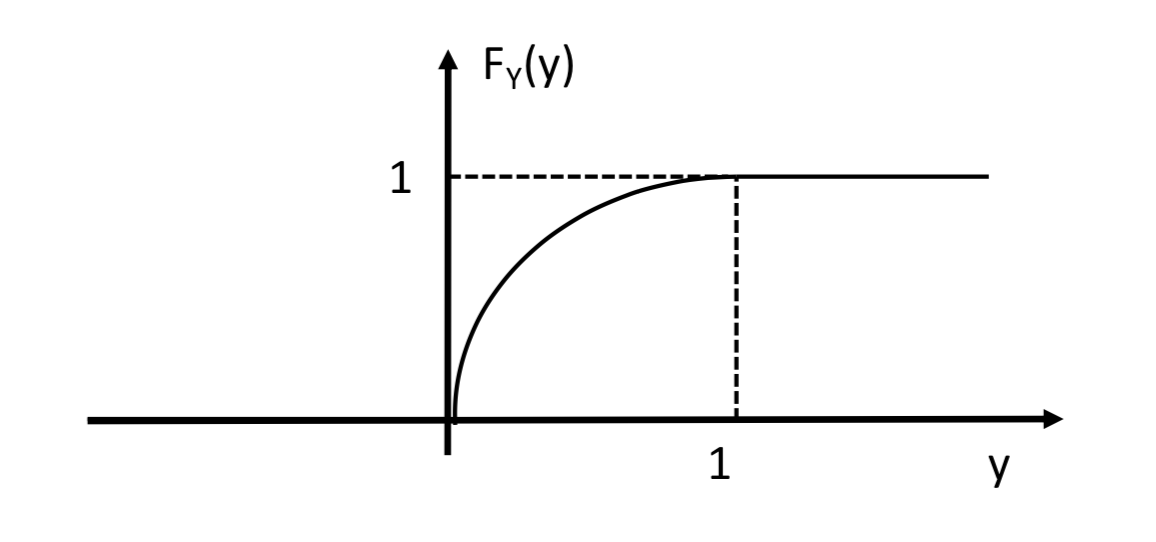
\includegraphics[scale=.4]{Figures/Fig13.png}
\end{center}
and, finally, we can obtain the density function of $Y$ as
\begin{eqnarray} 
\py = \frac{d F_Y(y)}{dy} =\begin{cases}
 \frac{1}{2\sqrt{y}} & \quad {\rm if} \quad 0<y<1 \\
 0 & \quad {\rm otherwise}  \\
\end{cases}  \nonumber
\end{eqnarray} 
\begin{center}
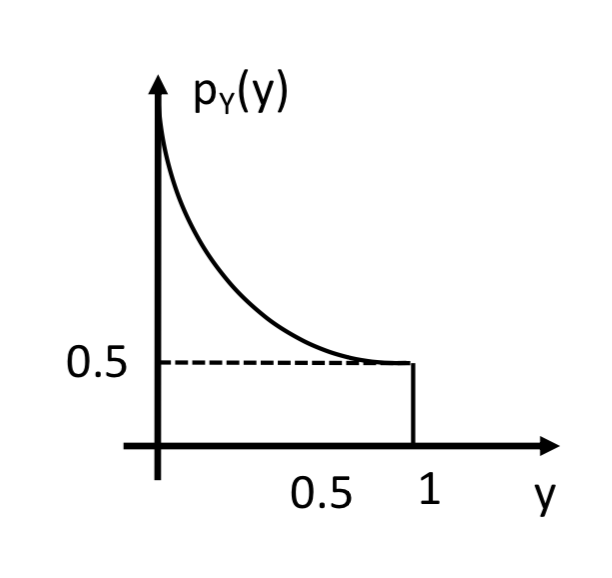
\includegraphics[scale=.4]{Figures/Fig14.png}
\end{center}
Now, let's try to generalize this procedure for any transformation
$$ Y = f(X) $$
being $f(\cdot)$ a strictly increasing function, so $f^{-1}(\cdot)$ exists.
\begin{enumerate}
    \item Compute the cumulative function of $Y$ (by means of $X$)
    \begin{eqnarray} 
    F_Y(y)  &= &  P\{Y<y\} =  P\{X<f^{-1}(y)\} = \int_{-\infty}^{f^{-1}(y)} \px dx = \nonumber \\ 
    & & F_X(f^{-1}(y)) - F_X(-\infty) = F_X(f^{-1}(y)) \nonumber
    \end{eqnarray} 
  Note: $F_X(-\infty) = 0$ for any cumulative distribution function  
    \item Compute the density distribution function (use the chain rule)
    \begin{eqnarray} 
    \py = \frac{d F_Y(y)}{dy} =  \frac{d F_X(f^{-1}(y))}{dy} = \frac{d F_X(x= f^{-1}(y))}{dx}  \frac{dx}{dy} = p_X(x= f^{-1}(y)) \frac{dx}{dy} \nonumber
    \end{eqnarray} 
    So, we obtain that 
    \begin{eqnarray}  \py = p_X(x= f^{-1}(y)) \frac{dx}{dy}  \nonumber \end{eqnarray} 
\end{enumerate}

This formula for the r.v. change can be generalized for any transformation function $f(\cdot)$ which is monotic (either strictly increasing or decreasing) as follows:
\begin{svgraybox}
\begin{equation} 
\py = p_X(x = f^{-1}(y))  \left| \frac{dx}{dy}\right| \label{eq:changeRV}
\end{equation} 
\end{svgraybox}

In fact, we can now use this formula over the previous example:
\begin{center}
\begin{tabular}{m{.2\textwidth}m{.5\textwidth}}
 \raisebox{-0.25ex}{$ Y = X^2$} &
 \begin{equation} 
\px = \begin{cases}
1 & {\rm if} \quad 0<x<1\\
0 & {\rm otherwise} 
\end{cases} \nonumber
\end{equation}
\end{tabular}
\end{center}
each term of the formula \eqref{eq:changeRV} is given by:
\begin{eqnarray} 
\left| \frac{dx}{dy}\right| = \left| \frac{df^{-1}(y)}{dy}\right| = \left| \frac{d\sqrt{y}}{dy}\right| = \frac{1}{2\sqrt{y}} \nonumber
\end{eqnarray} 

\begin{eqnarray} 
p_X(x = f^{-1}(y)) = p_X(x = \sqrt{y}) = \begin{cases}
1 & {\rm if} \quad 0<\sqrt{y}<1\\
0 & {\rm otherwise} 
\end{cases}  \nonumber
\end{eqnarray} 

So, we get

\begin{eqnarray} 
\py  = \frac{1}{2\sqrt{y}} p_X(x = \sqrt{y}) = \begin{cases}
\frac{1}{2\sqrt{y}} & {\rm if} \quad 0<y<1\\
0 & {\rm otherwise} 
\end{cases}  \nonumber
\end{eqnarray} 

In case the transformation function is not monotic, we have to divide the transformation into intervals where we get monotic transformations. That is, we have $Y = f(X)$ and $f(\cdot)$ is not monotic, then redefine the transformation as
\begin{eqnarray} 
Y = \begin{cases} 
f_1(X) & {\rm if } x_0 < x <x_1 \\
f_2(X) & {\rm if } x_1 < x <x_2 \\
\ldots  &  \\
f_N(X) & {\rm if } x_{N-1} < x <x_N \\
\end{cases}  \nonumber
\end{eqnarray}

where $f_1(\cdot),\ldots, f_N(\cdot) $ are monotic. Then, you can compute $\py$ as:
\begin{eqnarray} 
\py =  \sum_{n=1}^N p_X(x = f_n^{-1}(y))  \left| \frac{df_n^{-1}(y)}{dy}\right| \nonumber
\end{eqnarray} 

%%%%%%%%%%%%%%%%%%%%%%%%%%%%%%%%%%%%
\subsection{Some usual r.v. changes}

The demonstration of these changes is left as homework.

\begin{enumerate}
    \item SHIFTING of R.V. \\
    $ Y = X+a$, where $a$ is a known constant. Then,
    $$ \py =  p_X(x = y-a) $$
    when we are adding a constant to any r.v., we are shifting the distribution from the origin to the position of the constant
    
    \begin{center}
    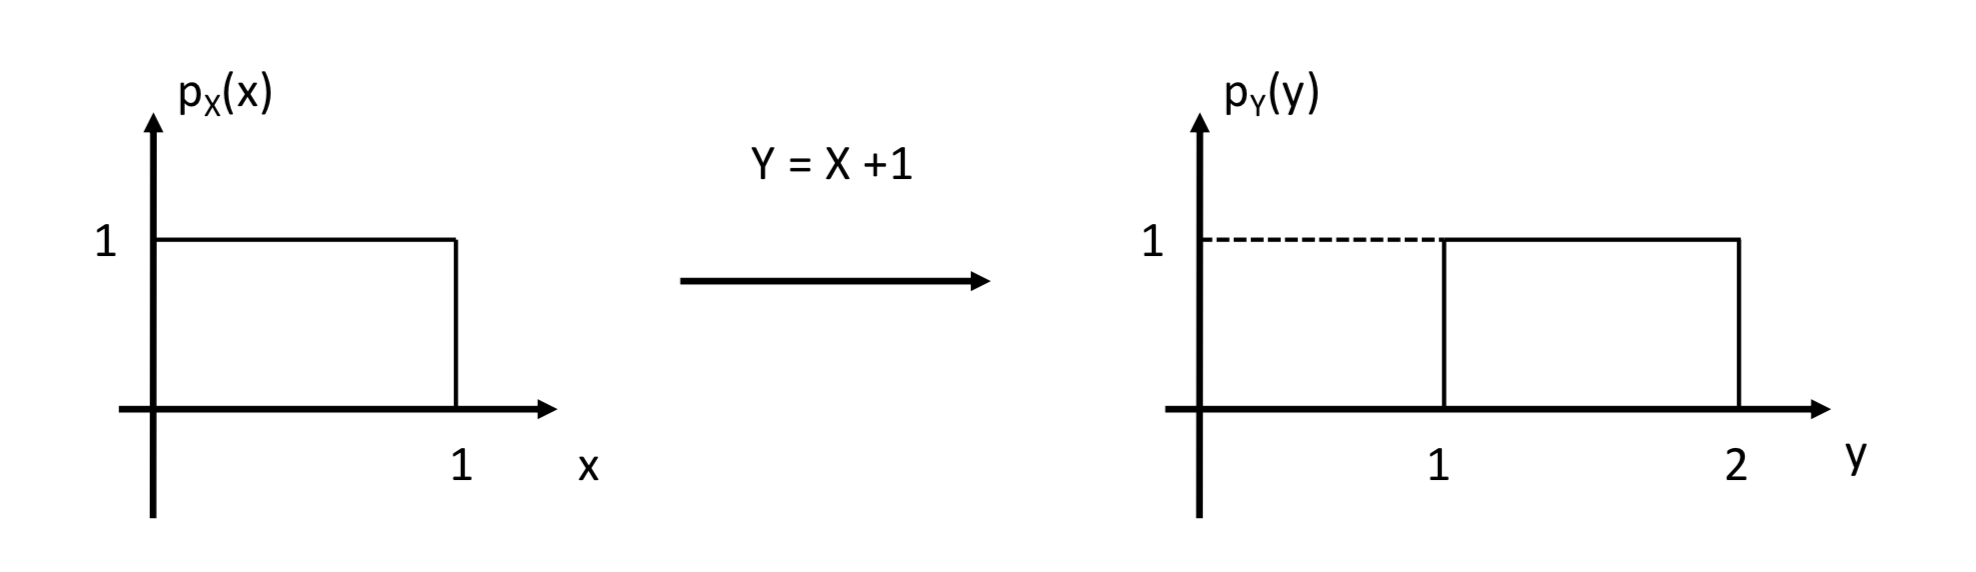
\includegraphics[scale=.3]{Figures/Fig15.png}
    \end{center}
    
    
    \item RESCALING of R.V.\\
    $ Y = aX$, where $a$ is a known constant. Then,
    $$ \py =  \frac{1}{a} p_X(x = \frac{y}{a}) $$
    in this case we are modifying both the support of the distribution function and its height.
    
    \begin{center}
    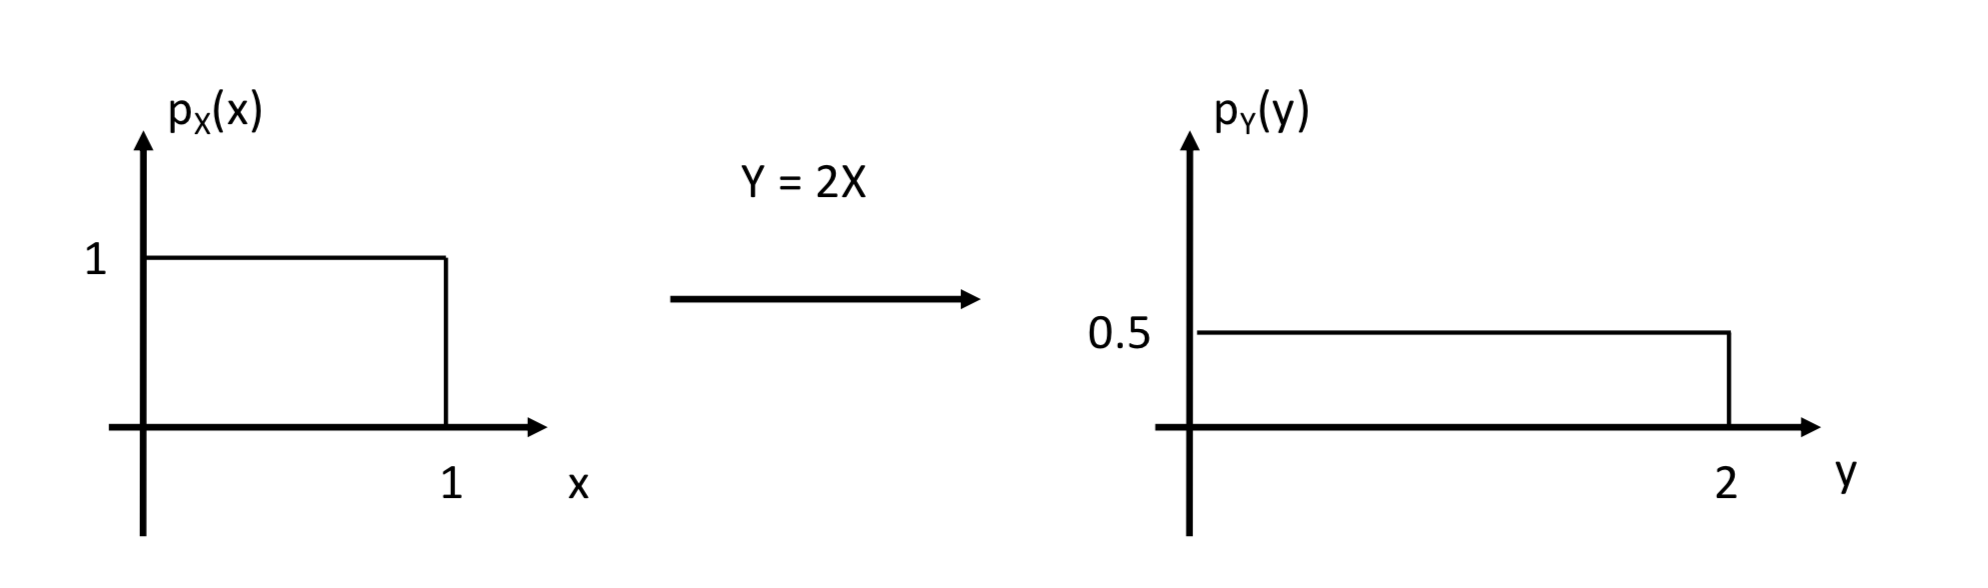
\includegraphics[scale=.3]{Figures/Fig16.png}
    \end{center}
    
\end{enumerate}

%%%%%%%%%%%%%%%%%%%%%% chapter.tex %%%%%%%%%%%%%%%%%%%%%%%%%%%%%%%%%
%
% sample chapter
%
% Use this file as a template for your own input.
%
%%%%%%%%%%%%%%%%%%%%%%%% Springer-Verlag %%%%%%%%%%%%%%%%%%%%%%%%%%
%\motto{Use the template \emph{chapter.tex} to style the various elements of your chapter content.}
\chapter{Appendix: Statistical Review}
\label{StatisticalReview} % Always give a unique label
% use \chaptermark{}
% to alter or adjust the chapter heading in the running head

%\abstract*{Each chapter should be preceded by an abstract (10--15 lines long) that summarizes the content. The abstract will appear \textit{online} at \url{www.SpringerLink.com} and be available with unrestricted access. This allows unregistered users to read the abstract as a teaser for the complete chapter. As a general rule the abstracts will not appear in the printed version of your book unless it is the style of your particular book or that of the series to which your book belongs.
%Please use the 'starred' version of the new Springer \texttt{abstract} command for typesetting the text of the online abstracts (cf. source file of this chapter template \texttt{abstract}) and include them with the source files of your manuscript. Use the plain \texttt{abstract} command if the abstract is also to appear in the printed version of the book.}

%\abstract{Each chapter should be preceded by an abstract (10--15 lines long) that summarizes the content. The abstract will appear \textit{online} at \url{www.SpringerLink.com} and be available with unrestricted access. This allows unregistered users to read the abstract as a teaser for the complete chapter. As a general rule the abstracts will not appear in the printed version of your book unless it is the style of your particular book or that of the series to which your book belongs.\newline\indent
%Please use the 'starred' version of the new Springer \texttt{abstract} command for typesetting the text of the online abstracts (cf. source file of this chapter template \texttt{abstract}) and include them with the source files of your manuscript. Use the plain \texttt{abstract} command if the abstract is also to appear in the printed version of the book.}

\section{Change of Random Variable}
\label{sec:1}
Let's consider we know the probability of a r.v. $X$, $\px$, and we now want to compute the probability density function of some variable $Y=f(X)$, that is, we need to calculate $\py$.

To understand how this new distribution or {\bf change of random variable} is calculated, let's firstly solve a particular case:

\begin{itemize}
\item $X$ is a uniform distribution in the interval $(0,1)$.


\begin{center}
\begin{tabular}{m{.5\textwidth}m{.4\textwidth}}
 \begin{equation} 
\px = \begin{cases}
1 & {\rm if} \quad 0<x<1\\
0 & {\rm otherwise} 
\end{cases} \nonumber
\end{equation} & 
\raisebox{-8ex}{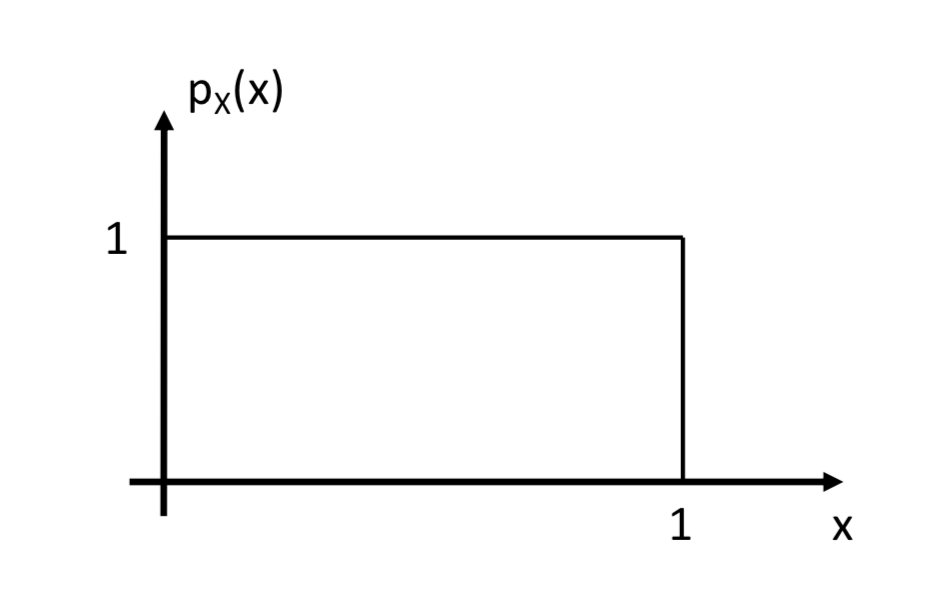
\includegraphics[scale=.25]{Figures/Fig11.png}} \\ 
\end{tabular}
\end{center}

\item $ Y = X^2$. Note that this change produces this transformation:
\begin{center}
\begin{tabular}{m{.5\textwidth}m{.4\textwidth}}
 \raisebox{-8ex}{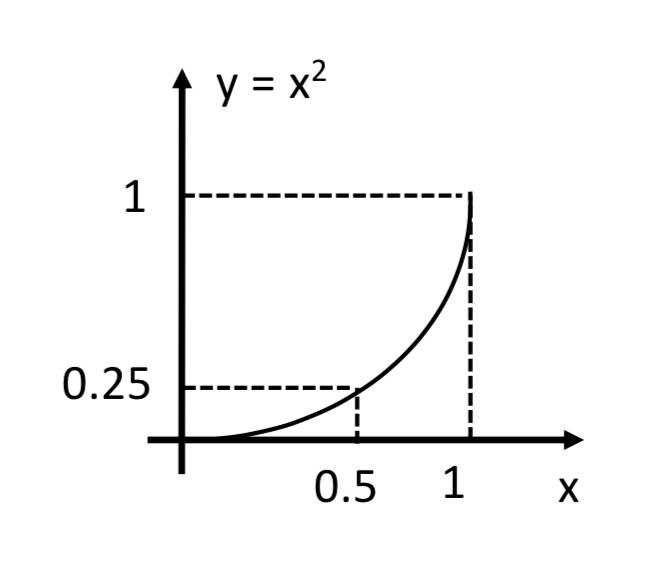
\includegraphics[scale=.4]{Figures/Fig12.png}} &
 \begin{tabular}{l|l}
$x$ & $y = x^2$ \\ \hline
0.1 & 0.01\\
0.2 & 0.04\\
0.5 & 0.25\\
... & ...\\
\end{tabular} 
\end{tabular}
\end{center}

The transformation function $f(\cdot)$ is strictly increasing. So there exists its inverse function $f^{-1}(\cdot)$.


\end{itemize}
To solve this change of r.v., we are going to use the fact that:

\begin{eqnarray}
P\{0<X<0.1\} &  = & P\{0<Y<0.01\}  \nonumber\\
P\{0<X<0.2\} &  = & P\{0<Y<0.04\}  \nonumber\\
P\{0<X<0.5\} &  = & P\{0<Y<0.25\}  \nonumber
\end{eqnarray}
or, in a general case, for any value of $X$, $x_0$, we have
$$ P\{0<X<x_0\}  = P\{0<Y<y_0\}$$
where $y_0=x_0^2$ or $x_0= \sqrt{y_0}$ 

So, we can compute the cumulative distribution function of the r.v. $Y$ as
$$ F_Y(y_0) =  P\{Y<y_0\} =  P\{X<\sqrt{y_0}\}$$

Now, as the cumulative function of $Y$ is expressed in terms of the r.v $X$, we can compute it!!!
\begin{eqnarray} 
F_Y(y_0) =  P\{X<\sqrt{y_0}\} = \int_{-\infty}^{\sqrt{y_0}} \px dx = 
\begin{cases}
\int_{-\infty}^{\sqrt{y_0}} 0 dx = 0 & \quad {\rm if} \quad y_0 <0 \\[2ex]
\int_0^{\sqrt{y_0}} 1 dx = \sqrt{y_0} & \quad {\rm if} \quad 0< y_0 <1 \\[2ex]
\int_0^{1} 1 dx = 1 & \quad {\rm if} \quad y_0 >1 \\
\end{cases}  \nonumber
\end{eqnarray}

So, we have that


\begin{eqnarray} 
F_Y(y_0) =\begin{cases}
 0 & \quad {\rm if} \quad y_0 <0 \\
 \sqrt{y_0} & \quad {\rm if} \quad 0< y_0 <1 \\
 1 & \quad {\rm if} \quad y_0 >1 \\
\end{cases}  \nonumber
\end{eqnarray} 
\begin{center}
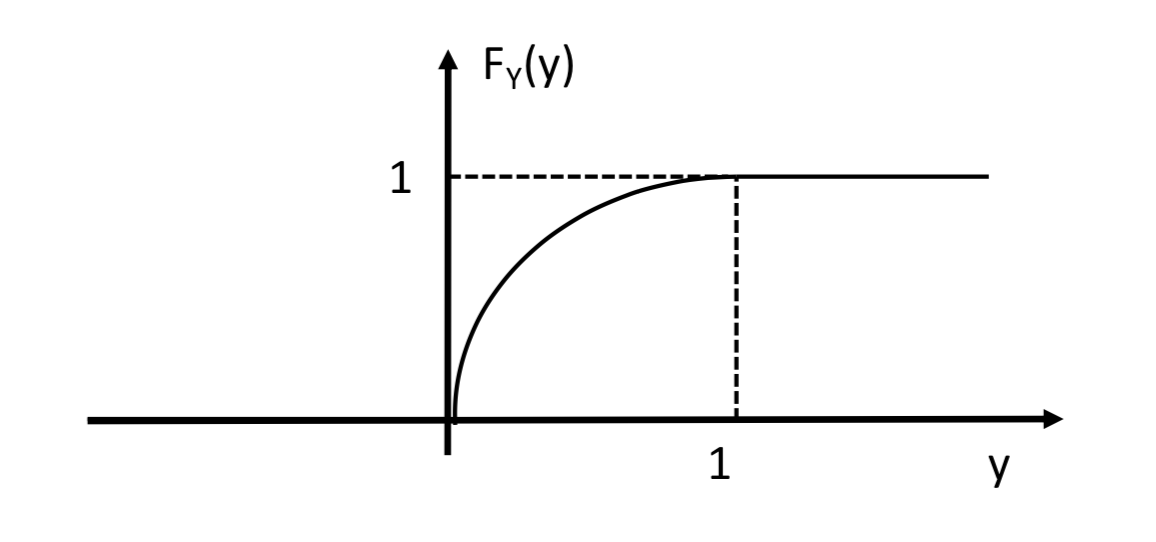
\includegraphics[scale=.4]{Figures/Fig13.png}
\end{center}
and, finally, we can obtain the density function of $Y$ as
\begin{eqnarray} 
\py = \frac{d F_Y(y)}{dy} =\begin{cases}
 \frac{1}{2\sqrt{y}} & \quad {\rm if} \quad 0<y<1 \\
 0 & \quad {\rm otherwise}  \\
\end{cases}  \nonumber
\end{eqnarray} 
\begin{center}
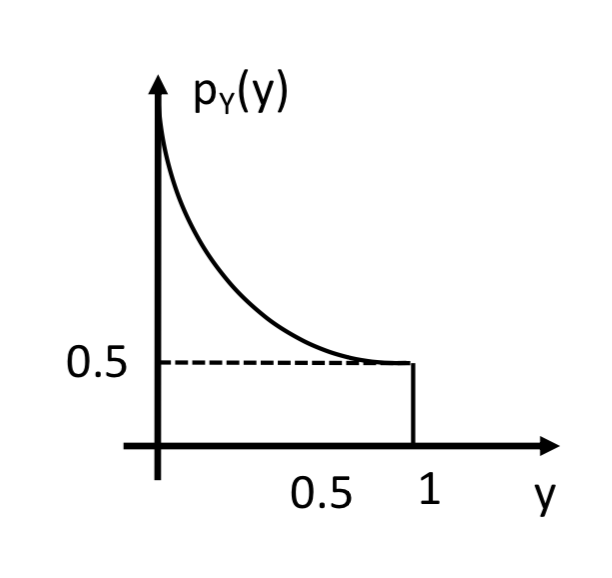
\includegraphics[scale=.4]{Figures/Fig14.png}
\end{center}
Now, let's try to generalize this procedure for any transformation
$$ Y = f(X) $$
being $f(\cdot)$ a strictly increasing function, so $f^{-1}(\cdot)$ exists.
\begin{enumerate}
    \item Compute the cumulative function of $Y$ (by means of $X$)
    \begin{eqnarray} 
    F_Y(y)  &= &  P\{Y<y\} =  P\{X<f^{-1}(y)\} = \int_{-\infty}^{f^{-1}(y)} \px dx = \nonumber \\ 
    & & F_X(f^{-1}(y)) - F_X(-\infty) = F_X(f^{-1}(y)) \nonumber
    \end{eqnarray} 
  Note: $F_X(-\infty) = 0$ for any cumulative distribution function  
    \item Compute the density distribution function (use the chain rule)
    \begin{eqnarray} 
    \py = \frac{d F_Y(y)}{dy} =  \frac{d F_X(f^{-1}(y))}{dy} = \frac{d F_X(x= f^{-1}(y))}{dx}  \frac{dx}{dy} = p_X(x= f^{-1}(y)) \frac{dx}{dy} \nonumber
    \end{eqnarray} 
    So, we obtain that 
    \begin{eqnarray}  \py = p_X(x= f^{-1}(y)) \frac{dx}{dy}  \nonumber \end{eqnarray} 
\end{enumerate}

This formula for the r.v. change can be generalized for any transformation function $f(\cdot)$ which is monotic (either strictly increasing or decreasing) as follows:
\begin{svgraybox}
\begin{eqnarray} 
\py = p_X(x = f^{-1}(y))  \left| \frac{dx}{dy}\right| \label{eq:changeRV}
\end{eqnarray} 
\end{svgraybox}

In fact, we can now use this formula over the previous example:
\begin{center}
\begin{tabular}{m{.2\textwidth}m{.5\textwidth}}
 \raisebox{-0.25ex}{$ Y = X^2$} &
 \begin{equation} 
\px = \begin{cases}
1 & {\rm if} \quad 0<x<1\\
0 & {\rm otherwise} 
\end{cases} \nonumber
\end{equation}
\end{tabular}
\end{center}



each term of the formula \eqref{eq:changeRV} is given by:
\begin{eqnarray} 
\left| \frac{dx}{dy}\right| = \left| \frac{df^{-1}(y)}{dy}\right| = \left| \frac{d\sqrt{y}}{dy}\right| = \frac{1}{2\sqrt{y}} \nonumber
\end{eqnarray} 

\begin{eqnarray} 
p_X(x = f^{-1}(y)) = p_X(x = \sqrt{y}) = \begin{cases}
1 & {\rm if} \quad 0<\sqrt{y}<1\\
0 & {\rm otherwise} 
\end{cases}  \nonumber
\end{eqnarray} 

So, we get

\begin{eqnarray} 
\py  = \frac{1}{2\sqrt{y}} p_X(x = \sqrt{y}) = \begin{cases}
\frac{1}{2\sqrt{y}} & {\rm if} \quad 0<y<1\\
0 & {\rm otherwise} 
\end{cases}  \nonumber
\end{eqnarray} 

In case the transformation function is not monotic, we have to divide the transformation into intervals where we get monotic transformations. That is, we have $Y = f(X)$ and $f(\cdot)$ is not monotic, then redefine the transformation as
\begin{eqnarray} 
Y = \begin{cases} 
f_1(X) & {\rm if } x_0 < x <x_1 \\
f_2(X) & {\rm if } x_1 < x <x_2 \\
\ldots  &  \\
f_N(X) & {\rm if } x_{N-1} < x <x_N \\
\end{cases}  \nonumber
\end{eqnarray}

where $f_1(\cdot),\ldots, f_N(\cdot) $ are monotic. Then, you can compute $\py$ as:
\begin{eqnarray} 
\py =  \sum_{n=1}^N p_X(x = f_n^{-1}(y))  \left| \frac{df_n^{-1}(y)}{dy}\right| \nonumber
\end{eqnarray} 

\subsection{Some usual r.v. changes}

The demonstration of these changes is left as homework.

\begin{enumerate}
    \item SHIFTING of R.V. \\
    $ Y = X+a$, where $a$ is a known constant. Then,
    $$ \py =  p_X(x = y-a) $$
    when we are adding a constant to any r.v., we are shifting the distribution from the origin to the position of the constant
    
    \begin{center}
    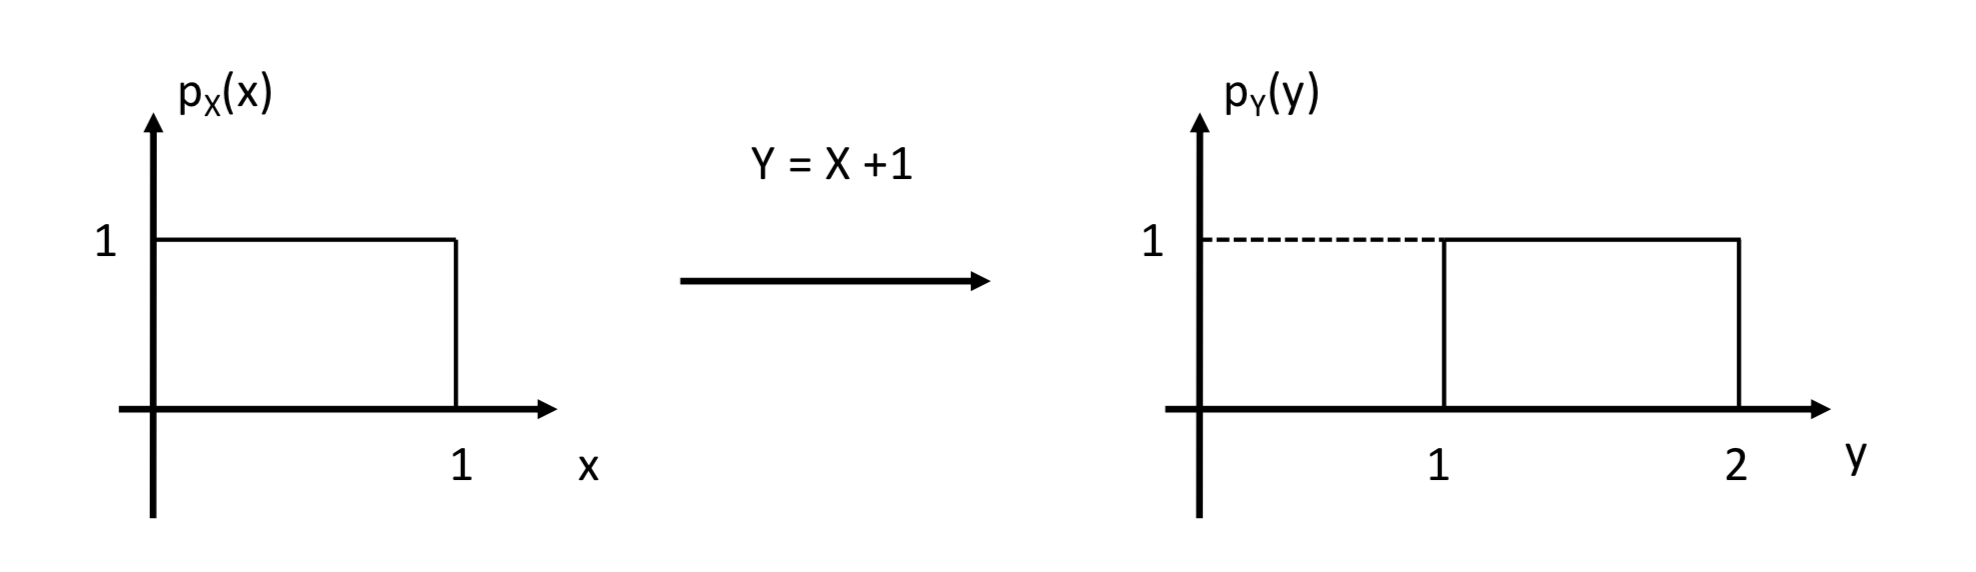
\includegraphics[scale=.3]{Figures/Fig15.png}
    \end{center}
    
    
    \item RESCALING of R.V.\\
    $ Y = aX$, where $a$ is a known constant. Then,
    $$ \py =  \frac{1}{a} p_X(x = \frac{y}{a}) $$
    in this case we are modifying both the support of the distribution function and its height.
    
    \begin{center}
    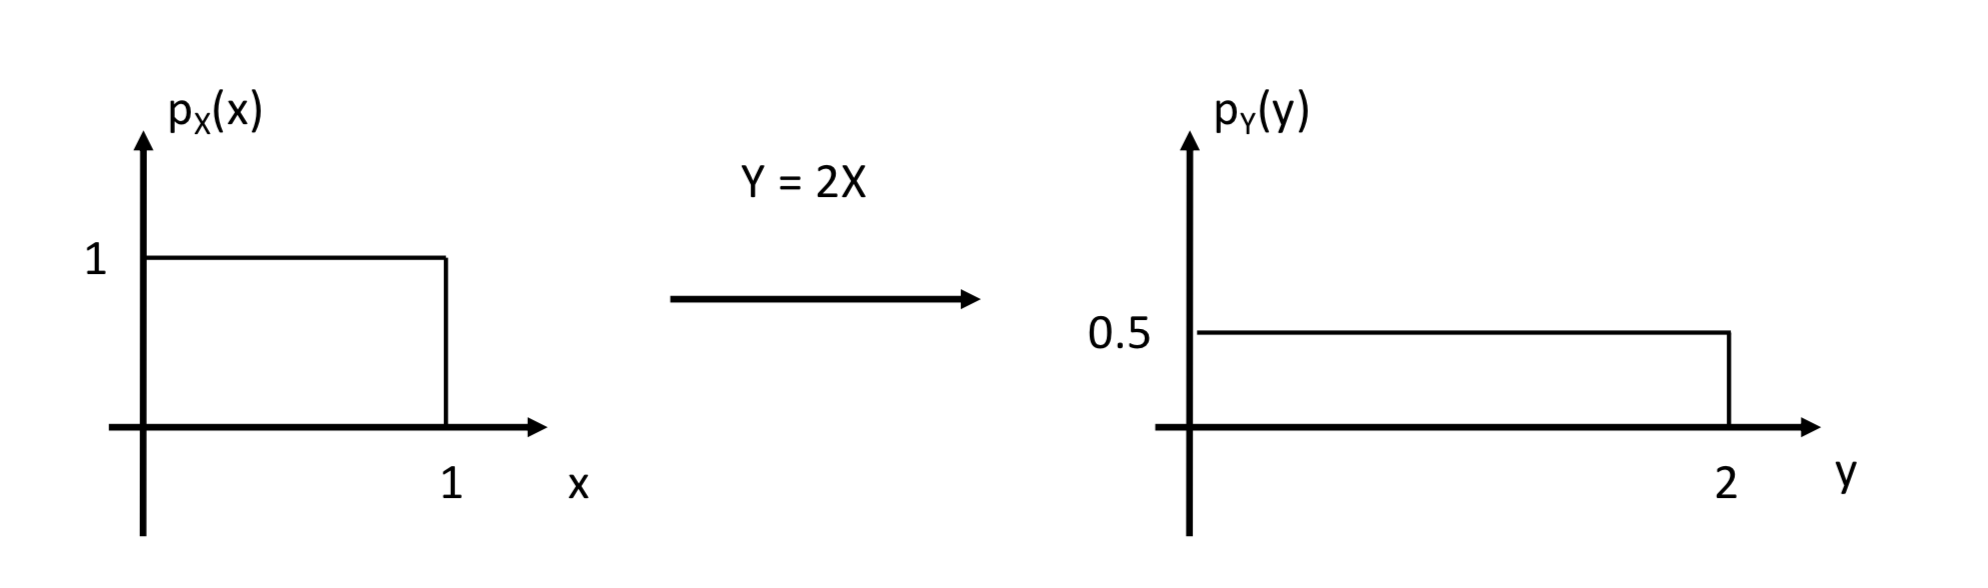
\includegraphics[scale=.3]{Figures/Fig16.png}
    \end{center}
    
\end{enumerate}




\backmatter%%%%%%%%%%%%%%%%%%%%%%%%%%%%%%%%%%%%%%%%%%%%%%%%%%%%%%%
%%%%%%%%%%%%%%%%%%%%%%%acronym.tex%%%%%%%%%%%%%%%%%%%%%%%%%%%%%%%%%%%%%%%%%
% sample list of acronyms
%
% Use this file as a template for your own input.
%
%%%%%%%%%%%%%%%%%%%%%%%% Springer %%%%%%%%%%%%%%%%%%%%%%%%%%

\Extrachap{Glossary}


Use the template \emph{glossary.tex} together with the Springer document class SVMono (monograph-type books) or SVMult (edited books) to style your glossary\index{glossary} in the Springer layout.


\runinhead{glossary term} Write here the description of the glossary term. Write here the description of the glossary term. Write here the description of the glossary term.

\runinhead{glossary term} Write here the description of the glossary term. Write here the description of the glossary term. Write here the description of the glossary term.

\runinhead{glossary term} Write here the description of the glossary term. Write here the description of the glossary term. Write here the description of the glossary term.

\runinhead{glossary term} Write here the description of the glossary term. Write here the description of the glossary term. Write here the description of the glossary term.

\runinhead{glossary term} Write here the description of the glossary term. Write here the description of the glossary term. Write here the description of the glossary term.
%\Extrachap{Solutions}

\section*{Problems of Chapter~\ref{intro}}

\begin{sol}{prob1}
The solution\index{problems}\index{solutions} is revealed here.
\end{sol}


\begin{sol}{prob2}
\textbf{Problem Heading}\\
(a) The solution of first part is revealed here.\\
(b) The solution of second part is revealed here.
\end{sol}


\printindex
%%%%%%%%%%%%%%%%%%%%%%%%%%%%%%%%%%%%%%%%%%%%%%%%%%%%%%%%%%%%%%%%%%%%%%

\end{document}





